 \documentclass[12pt, letterpaper, oneside]{article}
\usepackage{amsmath,amssymb,amscd,amsthm,eucal,curves,epic, graphicx, array}
\usepackage{booktabs}
\usepackage{framed}
\usepackage{pdfpages}
\usepackage[all]{xy}
\usepackage[latin1]{inputenc}
\usepackage{color}
\usepackage{floatflt}
\usepackage{tocloft}



\usepackage{rotating}



\definecolor{linkcol}{rgb}{0, 0, 0.7}
\usepackage[ linkcolor=linkcol, citecolor=linkcol, urlcolor= linkcol, colorlinks=true, hypertexnames=false]{hyperref}


\renewcommand{\familydefault}{\sfdefault} % switch to sans-serif fonts


\setlength{\parindent}{0in}
\setlength{\parskip}{4mm}

\setcounter{secnumdepth}{1}
\setcounter{tocdepth}{2}

\renewcommand{\labelenumi}{\theenumi )} % redefines enumerate labels to 1), 2) 3) etc.


%%%%%%%%%%%%%%%%%%%%%%%%%%%%
%   ENVIRONMENTS
%%%%%%%%%%%%%%%%%%%%%%%%%%%%

\swapnumbers

\theoremstyle{plain}
\newtheorem{theorem}{Theorem}[section]
\newtheorem{lemma}[theorem]{Lemma}
\newtheorem{proposition}[theorem]{Proposition}
\newtheorem{corollary}[theorem]{Corollary}

\newtheorem{FIT}[theorem]{First Isomorphism Theorem}
\newtheorem{SIT}[theorem]{Second Isomorphism Theorem}
\newtheorem{TIT}[theorem]{Third Isomorphism Theorem}


\newtheorem{FST}[theorem]{First Sylow Theorem}
\newtheorem{SST}[theorem]{Second Sylow Theorem}
\newtheorem{TST}[theorem]{Third Sylow Theorem}

\newtheorem{ZL}[theorem]{Zorn's Lemma}
\newtheorem{FTA}[theorem]{Fundamental Theorem of Arithmetic}
\newtheorem{FLT}[theorem]{Fermat's Last Theorem}
\newtheorem{FTALG}[theorem]{Fundamental Theorem of Algebra}
\newtheorem{HBT}[theorem]{Hilbert Basis Theorem}
\newtheorem{NNL}[theorem]{Noether Normalization Lemma}


\theoremstyle{definition}
\newtheorem{definition}[theorem]{Definition}
\newtheorem{cordef}[theorem]{Corollary/Definition}
\newtheorem{example}[theorem]{Example}
\newtheorem{examples}[theorem]{Examples}
\newtheorem{notation}[theorem]{Notation}
\newtheorem{remark}[theorem]{Remark}
\newtheorem{note}[theorem]{Note}
\newtheorem{conjecture}[theorem]{Conjecture}
\newtheorem{exercise}[theorem]{Exercise}
\newtheorem{problem}[theorem]{Problem}     
\newtheorem{definition/proposition}[theorem]{Definition/Proposition}  
\newtheorem{nn}[theorem]{}    
    
     

%%%%%%%%%%%%%%%%%%%%%%%%%%%%
%   MACROS
%%%%%%%%%%%%%%%%%%%%%%%%%%%%

\renewcommand{\bf}{\textbf}
\renewcommand{\it}{\textit}



%%% ARROWS

\newcommand{\noi}{\noindent}
\newcommand{\ra}{\rightarrow}
\newcommand{\la}{\leftarrow}
\newcommand{\lra}{\longrightarrow}
\newcommand{\Ra}{\Rightarrow}
\newcommand{\La}{\Leftarrow}
\newcommand{\hra}{\hookrightarrow}



%%% RINGS AND FIELDS

\newcommand{\N}{{\mathbb N}}
\newcommand{\Z}{{\mathbb Z}}
\newcommand{\Q}{{\mathbb Q}}
\newcommand{\R}{{\mathbb R}}
\newcommand{\C}{{\mathbb C}}
\newcommand{\HH}{{\mathbb H}}
\newcommand{\F}{{\mathbb F}}


%%% MORPHISM SETS

\newcommand{\Hom}{\mathrm{Hom}}
\newcommand{\Aut}{\mathrm{Aut}}
\newcommand{\Inn}{\mathrm{Inn}}
\newcommand{\Out}{\mathrm{Out}}
\newcommand{\End}{\mathrm{End}}
\newcommand{\Perm}{\mathrm{Perm}}
\newcommand{\Iso}{\mathrm{Iso}}
\newcommand{\Orb}{\mathrm{Orb}}




\newcommand{\Ob}{\mathrm{Ob}}

\newcommand{\id}{\mathrm{id}}
\newcommand{\inv}{\mathrm{inv}}

\renewcommand{\Im}{\operatorname{Im}}
\newcommand{\Ker}{\operatorname{Ker}}
\newcommand{\subgp}[1]{\langle#1\rangle}
\newcommand{\rank}{\operatorname{rank}}
\newcommand{\sgn}{\operatorname{sgn}}
\newcommand{\irr}{\operatorname{irr}}
\newcommand{\tr}{\operatorname{tr}}
\newcommand{\nil}{\operatorname{nil}}

\newcommand{\Gal}{\operatorname{Gal}}


%%% CATEGORIES

\newcommand{\CC}{{\mathcal C}}
\newcommand{\DD}{{\mathcal D}}
\newcommand{\Ab}{{\mathcal Ab}}
\newcommand{\Gr}{{\mathcal Gr}}
\newcommand{\Ring}{{\mathcal Ring}}
\newcommand{\Top}{{\mathcal Top}}
\newcommand{\Set}{{\mathcal Set}}
\newcommand{\Mod}{{\mathcal Mod}}


\newcommand{\Projfg}{\mathrm {Proj}^{fg}}
\newcommand{\Gro}{\mathrm {Gr}}

%%% VARIA

\newcommand{\bpm}{\begin{pmatrix}}
\newcommand{\epm}{\end{pmatrix}}

\newcommand{\benu}{\begin{enumerate}}
\newcommand{\eenu}{\end{enumerate}}

\newcommand{\bit}{\begin{itemize}}
\newcommand{\eit}{\end{itemize}}


\newcommand{\vs}{\vskip 5mm}
\newcommand{\msp}{\phantom{-}}     
\newcommand{\isep}[1][0]{\setlength{\itemsep}{#1 mm}}


%%%%%%%%%%%%%%%%%%%%%%%%%%%%
%   END MACROS
%%%%%%%%%%%%%%%%%%%%%%%%%%%%



\title{\Huge{\textbf{Notes on Algebra}}\\[3mm]
\Large{MTH 619/620}}
\author{}
\date{2015.09.01} % Delete this line to display the current date

%%%%%%%%%%%%%%%%%%%%%%%%%%%%
%   BEGIN DOCUMENT
%%%%%%%%%%%%%%%%%%%%%%%%%%%%

\begin{document}


\maketitle
\thispagestyle{empty}

%%%%%%%%%%%%%%%%%%%%%%%%%%%%
%  TABLE OF CONTENTS
%%%%%%%%%%%%%%%%%%%%%%%%%%%%



\newpage
\tableofcontents
\newpage












%%%%%%%%%%%%%%%%%%%%%%%%%%%%%%%
%%%%%%%%%%%%%%%%%%%%%%%%%%%%%%%
%%%
%%% MONOIDS AND GROUPS
%%%
%%%%%%%%%%%%%%%%%%%%%%%%%%%%%%%
%%%%%%%%%%%%%%%%%%%%%%%%%%%%%%%





\section{Monoids and groups}
\label{SEC_MON-GPS}

\begin{definition}
A \emph{monoid} is a set $M$ together with a map 
$$M\times M\to M, \ \ \ (x,  y) \mapsto x\cdot y$$
such that
\begin{itemize}
\item[(i)] $(x\cdot y)\cdot z=x\cdot (y\cdot z)\ \ \forall x, y, z\in M$ (associativity);
\item[(ii)] $\exists e\in M$ such that  
$$x\cdot e=e\cdot x = x$$  for all $x\in M$ ($e = $ the identity element of $M$).
\end{itemize}


\end{definition}


\vskip 5mm


\begin{examples}\hfill 
\begin{enumerate}
\label{EX_MONOIDS}

\item $\Z$ with addition of integers ($e=0$)

\item $\Z$ with multiplication of integers ($e=1$)

\item $M_{n}(\R)= \{\text{the set of all\ } n\times n \text{ \ matrices with coefficients in\  } \R \}$ 
with matrix multiplication ($e=I = $ the identity matrix)

\item $U =$ any set
$$P(U) := \{ \text{the set of all subsets of } U \} $$
$P(U)$ is a monoid with $A\cdot B := A\cup B$ and $e = \varnothing$.

\item Let $U= $ any set
$$F(U) := \{ \text{the set of all functions } f\colon U\to U\}$$
$F(U)$ is a monoid with multiplication given by composition of functions ($e = \mathrm{id}_{U} = $ the identity function).
\end{enumerate}
\end{examples}


\vskip 5mm


\begin{definition}
A monoid is \emph{commutative} if $x\cdot y = y\cdot x$ for all $x, y\in M$. 
\end{definition}

\begin{example}
Monoids 1), 2), 4) in \ref{EX_MONOIDS} are commutative; 3), 5) are not. 
\end{example}

\vskip 5mm

\begin{note}
Associativity implies that for $x_{1},  \dots, x_{k}\in M$ the 
expression 
$$x_{1}\cdot x_{2}\cdot \dots \cdot x_{k}$$ 
has the same value regardless how we place parentheses within it; e.g.: 
$$(x_{1}\cdot x_{2})\cdot (x_{3}\cdot x_{4})=((x_{1}\cdot x_{2})\cdot x_{3})\cdot x_{4}=
x_{1}\cdot ((x_{2}\cdot x_{3})\cdot x_{4})$$ etc.
\end{note}

\vs

\begin{note}
A monoid has only one identity element: if $e, e'\in M$ are identity elements then 
$$e=e\cdot e' = e'$$
\end{note}

\vs


\begin{definition}
A \emph{group} is a monoid $G$ such that for any $x\in G$ there is $y\in G$
satistying $x\cdot y= e = y\cdot x$.

The element $y$ is called the \emph{inverse} of $x$ and it is denoted by $x^{-1}$
(or by $-x$ in the additive notation).

A group $G$ is \emph{commutative} (or abelian) if $x\cdot y = y\cdot x$ for all $x, y\in G$.
\end{definition}

\vskip 5mm


\begin{examples}\hfill
\label{EX_GPS}
\begin{enumerate}

\item $\Z, \Q, \R, \C$ with addition

\item $\Q^{\ast}= \Q- \{0\}$, $\R^{\ast}= \R- \{0\}$, $\C^{\ast}= \C- \{0\}$ with multiplication

\item $GL_{n}(\R) = \{A\in M_{ n}(\R) \ | \ \det(A)\neq 0 \}$ with matrix multiplication \\
 (the $n\times n$ general linear group)

\item $SL_{n}(\R) = \{A\in M_{n}(\R)\ | \ \det(A) = 1\}$ with matrix multiplication \\
 (the $n\times n$ special linear group)
 
 \item Let $U = $ be any set and let 
 $$\Perm(U) := \{ f\colon U\to U \ | \  f \text{ is a bijection}\}$$
 $\Perm(U)$ with composition of functions is a group (the group of permutations of $U$)
  
\bf{Note.} If $U = \{1, 2, \dots, n\}$ then $\Perm(U)$ is called the \emph{symmetric group on
$n$  letters} and it is denoted by $S_{n}$.

\item[7)] Let $T = $ an equilateral triangle 
$$G_{T} = \{ I, R_{1}, R_{2}, S_{1}, S_{2}, S_{3} \}$$


\begin{figure}[h] 
   \centering
   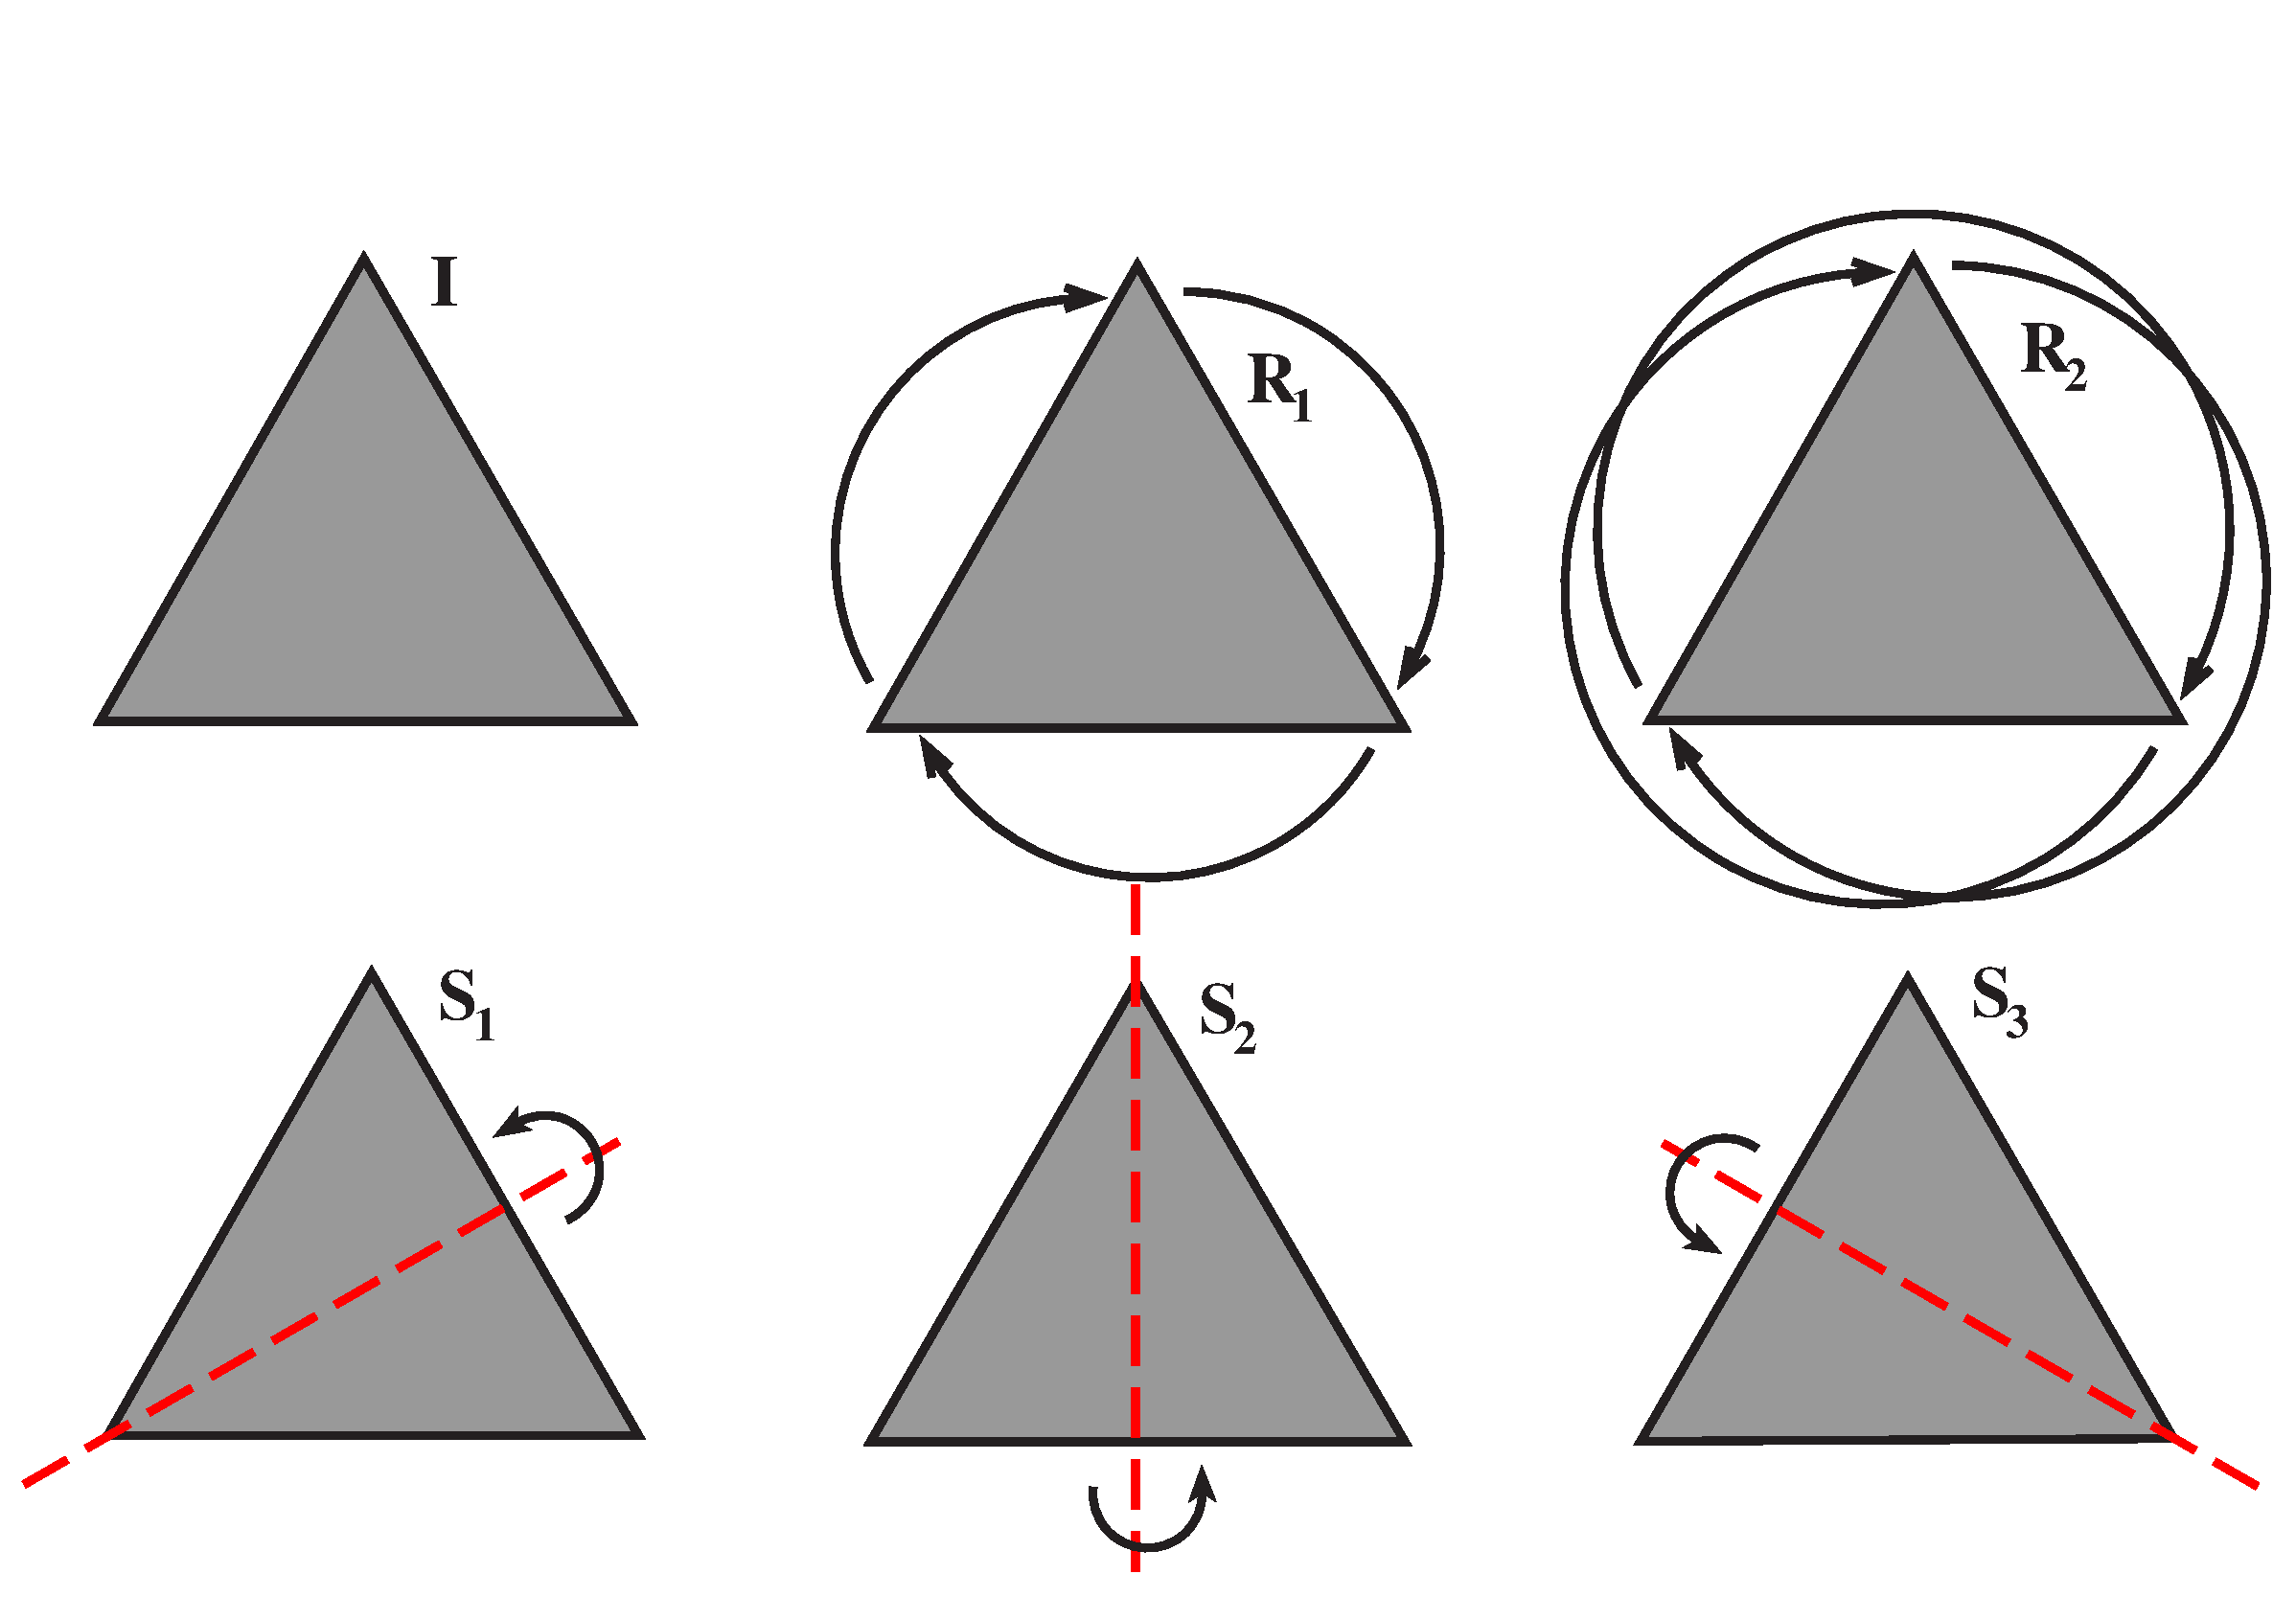
\includegraphics[width=3in]{pictures/triangle_symm.pdf} 
     \label{FIG_triangle_symm}
\end{figure}

$G_{T} = $  the group of symmetries of $T$.

\end{enumerate}
\end{examples}


\vskip 5mm

\begin{proposition}[Cancellation Law]
If $G$ is a group, $x, y, x\in G$ and 
$$xy = xz$$
then $y=z$.
\end{proposition}

\begin{proof}
\begin{gather*}
xy = xz \\ 
x^{-1}xy = x^{-1}xz\\
y = z
\end{gather*}
\end{proof}

\begin{note}
The cancellation law does not hold for monoids. E.g. in $M_{2}(\R)$ take
$$
A = \bpm 1 & 0 \\ 0 & 0\epm, \ B = \bpm 0 & 0 \\ 0 & 1\epm, \ C= \bpm 0 & 0 \\ 0 & 0 \epm
$$
Then $AB = AC$ but $A\neq C$.
\end{note}

\newpage



%%%%%%%%%%%%%%%%%%%%%%%%%%%%%%%
%%%%%%%%%%%%%%%%%%%%%%%%%%%%%%%
%%%
%%% SUBGROUPS
%%%
%%%%%%%%%%%%%%%%%%%%%%%%%%%%%%%
%%%%%%%%%%%%%%%%%%%%%%%%%%%%%%%


\section{Subgroups}
\label{SEC_SUBGROUPS}

\begin{definition}
\label{DEF_SUBGP}
If $G$ is a group then a \emph{subgroup} of $G$ is a subset $H\subseteq G$ such that

\vskip -13mm

\ 
\begin{itemize}
\isep
\item[(i)]  $e \in H$;
\item[(ii)] if $x, y\in H$ then $xy\in H$;
\item[(iii)] if $x\in H$ then $x^{-1}\in H$. 
\end{itemize}
\end{definition}

\vs


\begin{note}
A subgroup of a group is by itself a group. 
\end{note}


\vs

\begin{examples}\hfill
\label{EX_SUBGROUPS}

\vskip -13mm

\ 
\begin{enumerate}
\item  If $G$ is a group then $G$, $\{e\}$ are subgroups of $G$
\item $\Z$ is a subgroup of $\Q$, which is a subgroup of $\R$, which is a subgroup of $\C$.
\item $SL_{n}(\R)$ is a subgroup of $GL_{n}(\R)$
\item $H= \{ I, R_{1}, R_{2}\}$ is a subgroup of $G_{T}$
\end{enumerate}
\end{examples}

\vs

\begin{note}
If $\{ H_{i} \}_{i\in I}$ is a family of subgroups of $G$ then $\bigcap_{i\in I} H_{i}$ is also a subgroup 
of $G$.  
\end{note}

\vs

\begin{definition}
If $G$ is a group and $S$ is a subset of $G$ then denote
$$\subgp{S} = \text{the smallest subgroup of } G \text{ that contains } S$$
$\subgp{S}$ is the \emph{subgroup of $G$ generated by the set $S$}.
\end{definition}


\vskip 5mm

\begin{proposition}
If $S\subseteq G$ then $\subgp{S}$ consists of all elements of the form
$$x_{1}^{\pm 1}x_{2}^{\pm 1}\cdot \dots \cdot x_{k}^{\pm 1}$$
where $x_{1}, \dots, x_{k}\in S$.
\end{proposition}

\begin{proof}
Exercise.
\end{proof}

\vskip 5mm

\begin{definition}
A set $S\subseteq G$ \emph{generates} $G$ if $\subgp{S} = G$.
\end{definition}

\vskip 5mm

\begin{example}
$S= \{S_{1}, S_{2}\}$ generates $G_{T}$. 
\end{example}


\vskip 5mm

\begin{definition}
A group $G$ is \emph{finitely generated} if it is generated by some finite subset $S\subseteq G$.
\end{definition}


\vskip 5mm

\begin{note} \ 

\vskip -13mm

\ 
\begin{itemize}
\isep
\item Every finite group is finitely generated.

\item Some infinite groups are finitely generated; e.g. $\Z = \subgp{1}$.
\end{itemize}
\end{note}


\vskip 5mm 

\begin{definition}
A group $G$ is \emph{cyclic} if $G =\subgp{a}$ for some $a\in G$
\end{definition}

\vskip 5mm

\begin{note}
If $G$ is cyclic, $G= \subgp{a}$ then every element  $g\in G$ is of the form
$$g=a^{n}$$
for some $n\in \Z$  (where \ $a^{-n} := (a^{-1})^{n}$, $a^{0}= e$).
\end{note}

\vs

\begin{examples}\ 

\vskip -13mm

\ 
\begin{enumerate}
\item $\Z = \subgp{1}$ is cyclic.
\item $H := \{ I, R_{1}, R_{2}\}\subseteq G_{T}$ is cyclic:
$$H = \subgp{R_{1}} \text{ \ \ and \ \ }  H = \subgp{R_{2}}$$
\end{enumerate}
\end{examples}


%%%%%%%%%%%%%%%%%%%%%%%%%%%%%%%
%%%%%%%%%%%%%%%%%%%%%%%%%%%%%%%
%%%
%%% HOMOMORPHISM OF GROUPS
%%%
%%%%%%%%%%%%%%%%%%%%%%%%%%%%%%%
%%%%%%%%%%%%%%%%%%%%%%%%%%%%%%%


\newpage
\section{Homomorphisms of groups}
\label{SEC_GPHOM}


\begin{definition}
\label{DEF_GP_HOMOMRPHISM}
Let $G$, $H$ be groups. A function $f\colon G\to H$ is a \emph{group homomorphism}
if for any $a,b\in G$ we have 
$$f(ab)=f(a)f(b)$$
\end{definition}

\vs

\begin{proposition}
If $f\colon G\to H$ is a homomorphism of groups and  $e_{G}$, $e_{H}$ denote identity elements
in, respectively, $G$ and $H$ then
\begin{itemize}
\item[(i)] $f(e_{G})=e_{H}$
\item[(ii)] $f(a^{-1})=f(a)^{-1}$ for any $a\in G$.
\end{itemize}
\end{proposition}

\begin{proof}
(i) We have 
$$f(e_{G})=f(e_{G}\cdot e_{G})=f(e_{G})\cdot f(e_{G})$$
Multiplying this equation by $f(e_{G})^{-1}$ we obtain $e_{H}=f(e_{G})$.

(ii) Since by (i) we have $f(e_{G})=e_{H}$ therefore 
$$f(a)\cdot f(a^{-1})=f(a\cdot a^{-1})=f(e_{G})=e_{H}$$
It is now enough to multiply this equation from the left by $f(a)^{-1}$.
\end{proof}


\vs


\begin{definition}
A homomorphism $f\colon G\to H$ is an \emph{isomorphism} if there is a homomorphism
$g\colon H\to G$ such that $g\circ f = \id_{G}$ and $f\circ g = \id_{H}$.
\end{definition}


\vs 

\begin{proposition}
A map $f\colon G\to H$ is an isomorphism of groups iff $f$ is a homomorphism and a bijection.  
\end{proposition}

\begin{proof}
Exercise.
\end{proof}

\vs


\begin{definition}
If there exists an isomorphism $f\colon G\to H$ then we say 
that the groups $G$ and $H$ are \emph{isomorphic} and we write $G\cong H$.
\end{definition}

\begin{definition}
A homomorphism $f\colon G\to G$ is called an \emph{endomorphism} of $G$.
An isomorphism  $f\colon G\to G$ is called an \emph{automorphism} of $G$.
\end{definition}


\vs





\begin{examples}\ 

\vskip -13mm

\ 
\begin{enumerate}
\item $\id_{G}\colon G\to G$ is an automorphism of $G$.

\item $f\colon G\to G$, \ $f(g)=e\ \ \forall_{g\in G}\ $ is an endomorphism of $G$. 


\item If $f\colon G\to H$, $g\colon H \to K$ are homomorphisms then so is $g\circ f\colon G\to K$.

\item For $g\in G$ define 
$$c_{g}\colon G \to G, \ \ \ c_{g}(a) := gag^{-1}$$
Check: $c_{g}$ is an automorphism of $G$. Automorphisms of this form are called 
\emph{inner automorphisms} of $G$.  

\textbf{Note.} If $G$ is an abelian group then $c_{g}=\id_{G}$ for all $g\in G$.


\item Recall: $GL_{n}(\R) = \{ A\in M_{n} \ | \ \det(A)\neq 0 \}$,\ \ $\R^{\ast}= \R-\{0\}$

We have the determinant function:
$$\det \colon GL_{n}(\R) \to \R^{\ast}$$
Since $\det(AB)= \det(A)\cdot\det(B)$ this function is a homomorphism.

\item Let $G\subseteq GL_{2}(\R)$
$$G := \left\{ \left. \bpm 1 & r \\ 0 & 1 \\ \epm \ \ \right| \ \  r\in \R  \right\}$$
$G$ is a subgroup of $GL_{2}(\R)$:
$$
\bpm 1 & r \\ 0 & 1 \\ \epm\cdot \bpm 1 & s \\ 0 & 1 \\ \epm = \bpm 1 & r+s \\ 0 & 1 \\ \epm
$$
$$
\bpm 1 & r \\ 0 & 1 \\ \epm^{-1} = \bpm 1 & -r \\ 0 & \msp 1 \\ \epm $$

We have  homomorphisms:
$$f\colon \R \to G \ \ \text{and} \ \ g\colon \R \to G$$
where

$$f(r) = \bpm 1 & r \\ 0 & 1 \\ \epm, \ \ g\left( \bpm 1 & r \\ 0 & 1 \\ \epm\right) = r$$ 
Since $g\circ f = \id_{G}$, $f\circ g = \R$ we get $G\cong \R$.



\end{enumerate}
\end{examples}


\vs


\begin{definition}
If $G$ is a group then 
$$|G| := \text{the number of elements of G}$$
$|G|$ is called the \emph{order} of $G$.
\end{definition}


\vs 

\begin{example}
$|G_{T}| = 6$, $|\Z| = \infty$.
\end{example}

\vs

\begin{note}
If $G\cong H$ then $|G| = |H|$.
\end{note}




%%%%%%%%%%%%%%%%%%%%%%%%%%%%%%%
%%%%%%%%%%%%%%%%%%%%%%%%%%%%%%%
%%%
%%% KERNEL AND IMAGE
%%%
%%%%%%%%%%%%%%%%%%%%%%%%%%%%%%%
%%%%%%%%%%%%%%%%%%%%%%%%%%%%%%%


\newpage
\section{The kernel and  the image of a homomorphism}
\label{SEC_KERIM}


\begin{proposition}
Let $f\colon G\to H$ be a homomorphism.

\vskip -13mm

\ 
\benu
\isep
\item If $G'$ is a subgroup of $G$ then $f(G')$ is a subgroup of $H$.
\item If $H'$ is a subgroup of $H$ then $f^{-1}(H')$ is a subgroup of $G$.
\eenu
\end{proposition}


\begin{proof}
Exercise.
\end{proof}

\vs


\begin{definition}
If $f\colon G\to H$ is a homomorphism then 

\vskip -13mm

\ 
\bit
\isep
\item the \emph{image} of $f$ is the subgroup 
$$\Im(f) := f(G) \subseteq H$$ 
\item the \emph{kernel} of $f$ is the subgroup 
$$\Ker(f) := f^{-1}(e_{H})\subseteq G$$
\eit
\end{definition}


\vs

\begin{note}
$f\colon G\to H$ is an epimorphism (onto) iff $\Im(f) = H$. 
\end{note}

\vs

\begin{proposition}
\label{PROP_MONOGRKER}
$f\colon G\to H$ is a monomorphism (1-1) iff $\Ker(f) = \{e_{G}\}$
\end{proposition}

\begin{proof}
$(\Ra)$ We have $f(e_{G})= e_{H}$. Thus if $f$ is 1-1 then $f(g)=e_{H}$ only if 
$g=e_{H}$. In other words we have then $\Ker(f) = \{e_{H}\}$.  

$(\La)$ Assume that $\Ker(f) = \{e_{G}\}$ and let $f(a)= f(b)$ for some $a, b\in G$. 
We have:
$$f(ab^{-1})= f(a)f(b)^{-1} = e_{H}$$
so $ab^{-1}\in \Ker(f)$. Therefore $ab^{-1}= e_{G}$, and so $a = b$. 

\end{proof}

\vs 

\begin{problem}
Let $G$ be a group, and let $H$ be a subgroup of $G$. Is there a homomorphism 
$$f\colon G \to K$$
such that $\Ker(f) = H$?
\end{problem}

\vs

\begin{note}
The dual problem is trivial: if $H$ is a subgroup of $G$ then we have the 
inclusion homomorphism
$$i\colon H \hra G$$
and $\Im(i) = H$. It follows that any subgroup of $G$ is an image of some homomorphism.  
\end{note}

\vs

\begin{definition}
A subgroup $H\subseteq G$ is a \emph{normal subgroup} if for every $h\in H$ 
we have 
$$aha^{-1} \in H \  \ \ \forall a\in G$$
\end{definition} 

\begin{notation}
If $H$ is a normal subgroup of $G$ then we write $H\lhd G$
\end{notation}

\vs 

\begin{proposition}
If $f\colon G\to H$ is a homomorphism then $\Ker(f)$ is a normal subgroup of $G$.
\end{proposition}

\begin{proof}
If $a\in G$, $h\in \Ker(f)$ then 
$$f(aha^{-1}) = f(a)f(h)f(a)^{-1} = f(a)\cdot e\cdot f(a)^{-1} = f(a)f(a)^{-1} = e$$
so $aha^{-1}\in \Ker(f)$.
\end{proof}


\vs 

\begin{examples}\hfill

\vskip -13mm

\ 
\benu
\item Any subgroup of an abelian group is normal.
\item $H:=\{I, R_{1}, R_{2} \}$ is a normal subgroup of $G_{T}$ (check!). 
\item $K:=\{I , S_{1}\}$ is not a normal subgroup of $G_{T}$ (check!). As a consequence 
$K$ cannot be the kernel of any homomorphism $G_{T} \to G$.
\eenu
\end{examples}






%%%%%%%%%%%%%%%%%%%%%%%%%%%%%%%
%%%%%%%%%%%%%%%%%%%%%%%%%%%%%%%
%%%
%%% KERNEL AND IMAGE
%%%
%%%%%%%%%%%%%%%%%%%%%%%%%%%%%%%
%%%%%%%%%%%%%%%%%%%%%%%%%%%%%%%


\newpage
\section{Normal subgroups, cosets and quotient groups}
\label{SEC_COSETS}

\textbf{Recall.} If $f\colon G\to K$ is a homomorphism then $\Ker(f)$ is a normal subgroup 
of $G$. 

\textbf{Next goal:} If $H$ is a normal subgroup of $G$ then there is a homomorphism 
$f\colon G\to K$ such that $H = \Ker(f)$. 



\vs

\vs 


\begin{definition}
If $H$ is a subgroup of $G$ then a \emph{left coset} of $H$ in $G$ is a subset of $G$
of the form 
$$aH := \{ah \ | \ h\in H\}$$
for some $a\in G$. 

A \emph{right coset} of $H$ in $G$ is a subset of $G$
of the form 
$$Ha := \{ha \ | \ h\in H\}$$
for some $a\in G$. 
\end{definition}


\begin{example} \ 
\label{EX_COSET}

\vskip -10mm

\ 

Recall: $G_{T} = \{I, R_{1}, R_{2}, S_{1}, S_{2}, S_{3} \}$. 
Take $H := \{I, S_{1}\} $. We have:

$IH = \{I\cdot I, I\cdot S_{1}\} = \{I, S_{1}\} = H $ \\
$S_{1}H = \{ S_{1}\cdot I, S_{1}\cdot S_{1}\} = \{S_{1}, I\}$ \\
$S_{2}H = \{ S_{2}\cdot I, S_{2}\cdot S_{1}\} = \{S_{2}, R_{2}\}$ \\
$S_{3}H = \{ S_{3}\cdot I, S_{3}\cdot S_{1}\} = \{S_{3}, R_{1}\}$ \\
$R_{1}H = \{ R_{1}\cdot I, R_{1}\cdot S_{1}\} = \{R_{1}, S_{3}\}$ \\
$R_{2}H = \{ R_{2}\cdot I, R_{2}\cdot S_{1}\} = \{R_{2}, S_{2}\}$ \\


Note:  $IH = S_{1}H$, $S_{2}H = R_{2}H$, $S_{3}H = R_{1}H$

\end{example}

\vs

\begin{lemma}
\label{LEMMA_COSETS}
If $G$ is a group and $H$ is a subgroup of $G$ then 
$$aH = bH \ \ \ \text{iff} \ \ \ a^{-1}b \in H$$
\end{lemma}

\begin{proof}
$(\Ra)$ Let $aH = bH$. Since $e\in H$ thus 
$$b = be \in bH = aH$$
so $b = ah$ for some $h\in H$. Therefore $a^{-1}b = h \in H$.

\vs

$(\La)$ Assume that  $a^{-1}b\in H$. For any $h\in H$ we have 
$$ah = a(a^{-1}b)(a^{-1}b)^{-1}h  = b((a^{-1}b)^{-1})h \in bH$$
This gives: $aH \subseteq bH$. Also for any $h\in H$ we have:
$$bh = (aa^{-1})bh = a(a^{-1}b)h \in aH$$
so $bH\subseteq aH$. Therefore $aH= bH$.
\end{proof}


\vs 

\begin{proposition}
If $H$ is a subgroup of $G$ then for any  $a, b\in G$ either
$$aH = bH \ \ \ \text{or} \ \ \ aH\cap bH = \varnothing $$
\end{proposition}

\begin{proof}
Let $aH\cap bH \neq \varnothing $ and let $c\in aH\cap bH$. Then
$$ah_{1} =  c = bh_{2}$$
for some $h_{1}, h_{2}\in H$. This gives 
$$a^{-1}b = h_{1}h_{2}^{-1} \in H$$
and so $aH = bH$ by (\ref{LEMMA_COSETS}).
\end{proof}


\vs

\begin{corollary}
\label{COR_DISJCOSETS}
If $H$ is a subgroup of $G$ then every element of $G$ belongs to one and only left 
coset of $H$.
\end{corollary}


\vs



\begin{note}
In general $aH\neq Ha$. For example, If $H\subseteq G_{T}$, 
$H= \{I, S_{1}\}$ then 
$$S_{2}H = \{S_{2}, R_{2}\}, \ \ \ HS_{2} = \{S_{2}, R_{1}\}$$ 

\end{note}



\vs


\begin{proposition}
\label{PROP_LRCOSETS}
A subgroup $H$ of $G$ is normal iff 
$$aH = Ha \ \ \ \forall a\in G$$
\end{proposition}


\begin{proof}
Exercise.
\end{proof}


\vs

\begin{notation}
If $H$ is a subgroup of $G$ then 
$$G/H := \text{the set of all left cosets of } H \text{ in } G$$ 
\end{notation}

\vs

\begin{nn}\textbf{Multiplication of cosets. }
\label{NN_COSETMULT}
Let $H\subseteq G$, $aH, bH \in G/H$. Define
$$aH \cdot bH := (ab)H$$
\end{nn}

\vs

\begin{note}
In general this is not well defined, i.e. we may have $aH = a'H$, $bH= b'H$ but 
$(ab)H \neq (a'b')H$. 

For example,  take $H=\{ I, S_{1}\}\subseteq G_{T}$. Recall:
$$S_{2}H = R_{2}H = \{S_{2}, R_{2}\}, \ S_{3}H = R_{1}H = \{S_{3}, R_{1}\}$$
However:
$$(S_{2}S_{3})H = R_{1}H = \{R_{1}, S_{2}\}$$
$$(R_{2}R_{1})H = IH = \{I, S_{1}\}$$

\end{note}

\vs

\begin{proposition}
If $H$ is a normal subgroup of $G$ then the multiplication of cosets given in (\ref{NN_COSETMULT})
is well defined.
\end{proposition}


\begin{proof}
If $H\lhd G$ then by  (\ref{PROP_LRCOSETS}) we have $aH = Ha\ \ \forall_{a\in G}$.

Let $aH = a'H$, $bH = b'H$. Then
$$(ab)H = a(bH) = a(b'H) = a(Hb') = (aH)b' = (a'H)b' = a'(b'H)=(a'b')H$$ 
\end{proof}

\vs 

\begin{cordef}
If $H\lhd G$ then $G/H$ is a group with multiplication defined by (\ref{NN_COSETMULT}). The identity 
elements in $G/H$ is the coset $eH = H \in G/H$. The inverse of a coset $aH$ is the coset $a^{-1}H$.

The group $G/H$ is called the \emph{quotient group} (or the \emph{factor group}) of $G$ by $H$. 
\end{cordef}

\vs

\begin{example}\ 

Take $\Z$, the additive group of integers. Since $\Z$ is abelian every its subgroup is normal. 
For $n\in \Z$, $n\geq 2$ define
$$n\Z = \{ na \ | \ a \in \Z \}$$
e.g. $2\Z= \{\dots -4, -2, 0, 2, 4, \dots\}$, $5\Z = \{\dots , -10, -5, 0, 5, 10, \dots \}$

Note: $n\Z$ is a subgroup of $\Z$.

Cosets of $n\Z$ in $\Z$:
$$k+n\Z = \{ k+na \ | \ a\in \Z \}$$
e.g. $1+ 5\Z= \{\dots -9, -4, 1, 6, 11, \dots\}$, $3+5\Z = \{\dots , -7, -2, 3, 8, 13, \dots \}$

Note: $k+n\Z = l+ n\Z$ iff $(k-l) \in n\Z$ i.e. iff $k = l+ na$ for some $a\in \Z$. 

E.g.: 
$$1 + 5\Z = 6 + 5\Z = 11 + 5\Z = -4+5\Z$$

Recall:  if $n, k\in \Z$ then there is a unique number $l\in\{0, 1, \dots, n-1 \}$ such that 
$$k = l+ na $$
for some $a\in \Z$. Thus every coset of $n\Z$ can be uniquely written as 
$l+n\Z$ where $l\in \{0, 1, \dots, n-1\}$.


Denote $\bar{l} := l+n\Z$. Then 
$\Z/n\Z = \{\bar{0}, \bar{1}, \dots, \overline{n-1}\}$

The addition table in $\Z/5\Z$:

\begin{center}
\begin{tabular}{b{3mm} |b{3mm} b{3mm} b{3mm} b{3mm} b{3mm} }
+                &  $\ \bar{0}$ &  $\bar{1}$  &  $\bar{2}$ &  $\bar{3}$ &  $\bar{4}$ \\ \midrule
$\bar{0}$  &  $\ \bar{0}$ &  $\bar{1}$  &  $\bar{2}$ &  $\bar{3}$ &  $\bar{4}$ \\[3pt] 
$\bar{1}$  &  $\ \bar{1}$ &  $\bar{2}$  &  $\bar{3}$ &  $\bar{4}$ &  $\bar{0}$ \\[3pt]  
$\bar{2}$  &  $\ \bar{2}$ &  $\bar{3}$  &  $\bar{4}$ &  $\bar{0}$ &  $\bar{1}$ \\[3pt]  
$\bar{3}$  &  $\ \bar{3}$ &  $\bar{4}$  &  $\bar{0}$ &  $\bar{1}$ &  $\bar{2}$ \\[3pt]   
$\bar{4}$  &  $\ \bar{4}$ &  $\bar{0}$  &  $\bar{1}$ &  $\bar{2}$ &  $\bar{3}$ \\[3pt]  
\end{tabular}
\end{center}


Recall: A group $G$ is cyclic if it is generated by a single element: $G=\subgp{a}$ for some 
$a\in G$. 

Note: For every $n$ the group $\Z/n\Z$ is cyclic: $\Z/n\Z = \subgp{\bar{1}}$. 

\end{example}



\vs

\begin{note}
If $H\lhd G$ then we have a homomorphism
$$\pi\colon G \to G/H, \ \ \ \pi(a) := aH$$
This is the  \emph{canonical epimorphism} of $G$ onto $G/H$.

We have:
\begin{align*}
\Ker(\pi) & = \{a\in G \ | \  \pi(a) = eH \} \\
&  = \{ a\in G \ | \ aH = eH \} \\
& = \{ a\in G \ |  \ e^{-1}a \in H \} \\
& = \{a\in G \ | \ a\in H \} \\
& = H \\
\end{align*}
\end{note}

\vs 

\begin{corollary}
A subgroup $H\subseteq G$ is the kernel of some homomorphism $f\colon G \to K$ iff
$H$ is a normal subgroup
\end{corollary}

\vs




%%%%%%%%%%%%%%%%%%%%%%%%%%%%%%%
%%%%%%%%%%%%%%%%%%%%%%%%%%%%%%%
%%%
%%% ISOMORPHISMS THEOREMS
%%%
%%%%%%%%%%%%%%%%%%%%%%%%%%%%%%%
%%%%%%%%%%%%%%%%%%%%%%%%%%%%%%%


\newpage
\section{Isomorphism theorems}
\label{SEC_ISOTHMS}



\begin{theorem}
\label{THM_HOMOMFACT}
If $f\colon G\to H$ is a homomorphism then there is a unique  homomorphism 
$$\bar{f}\colon G/\Ker(f) \to H$$
such that the following diagram commutes:
$$
\xymatrix{
G \ar[rr]^{f} \ar[dd]_{\pi} & & H \\
\\
G/\Ker(f)\ar@{-->}[rruu]_{\bar{f}} & \\
}
$$
Moreover, $\bar{f}$ is a monomorphism and $\Im(\bar{f})= \Im(f)$. 
\end{theorem}


\begin{proof}
Denote: $K:=\Ker(f)$. Define
$$\bar{f}\colon G/K \to H, \ \ \ \bar{f}(aK) := f(a)$$
We have:

1) $\bar{f}$ is well defined:

If $aK = bK$ then $a^{-1}b\in K$, so $f(a^{-1}b) = e$. Thus
$$f(b) = f(aa^{-1}b) = f(a)f(a^{-1}b) = f(a)$$

2) $\bar{f}$ is a homomorphism (check).


3) $\bar{f}$ is a unique homomorphism satisfying $\bar{f}\circ \pi = f$

Indeed, if $g\colon G/K \to H$ is some other homomorphism and $g\circ \pi = f$
then  
$$f(a) = g\circ \pi(a) = g(aK)$$ 
and so $g(aK) = \bar{f}(aK)$ for all $aK \in G/K$. 

4) $\bar{f}$ is 1-1:

We need: $\Ker(\bar{f}) = \{eK\}$. \newline
We have: if $\bar{f}(aK) = e$ then  $f(a) = e$, so $a\in K$ and so $aK = eK$. 

5) $\Im(f) = \Im(\bar{f})\ $ (obvious). 

\end{proof}


\vs

\begin{FIT}
\label{THM_FIT}
If $f\colon G\to H$ is an epimorphism then 
$$G/\Ker(f) \cong H$$
\end{FIT}

\begin{proof}
Take the map $\bar{f}\colon G/\Ker(f) \to H$. Then $\Im(\bar{f})= \Im(f) = H$, so $\bar{f}$ is 
an epimorphism. Also, $\bar{f}$ is 1-1. Therefore $\bar{f}$ is a bijective homomorphism 
and thus it is an isomorphism. 
\end{proof}


\vs

\begin{example} \ 

Recall:
$$GL_{n}(\R) = \{ A\in M_{n}(\R) \ |\ \det(A)\neq 0 \}$$
$$SL_{n}(\R) = \{ A\in M_{n}(\R) \ |\ \det(A) = 1 \}$$ 
$SL_{n}(\R)$ is a normal subgroup of $GL_{n}(\R)$. 

We have the homomorphism
$$\det \colon GL_{n}(\R) \to \R^{\ast}$$
Since this is an epimorphism and $\Ker(\det)= SL_{n}(\R)$ we get
$$GL_{n}(\R)/SL_{n}(\R)\cong \R^{\ast}$$

\end{example}

\vs 

\begin{theorem}
If $G$ is a cyclic group then $G\cong \{ e\}$ or $G\cong \Z$ or $G\cong \Z/n\Z$ for some $n\geq 2$.
\end{theorem}

\begin{proof}
Let $G = \subgp{a}$ for some $a\in G$. Define
$$f\colon \Z \to G, \ \ \ f(n) := a^{n}$$
Notice that 

\vskip -13mm

\ 
\begin{enumerate}
\setlength{\itemsep}{1pt}
\item $f$ is a homomorphism
\item $f$ is onto. 
\end{enumerate}
Thus by the First Isomorphism Theorem $G\cong \Z/\Ker(f)$.

Check: all subgroups  $H\subseteq \Z$ are of the form $H= n\Z$ for some $n\geq 0$. 

It follows that $G\cong \Z/n\Z$ for some $n\geq 0$. Also:

\vskip -13mm

\ 
\begin{itemize}
\item if $n=0$ then $n\Z = 0\Z = \{0\}$ and $G\cong \Z/\{0\} \cong \Z$

\item if $n =1$ then $n\Z = 1\Z = \Z$ and $G\cong \Z/\Z \cong \{e\}$

\item if $n\geq 2$ then $G\cong \Z/n\Z$.

\end{itemize}


\end{proof}


\vs 

\begin{notation}
If $H, K$ are subgroups of $G$ then 
$$HK := \{ hk \in G \ | \ h\in H, k\in K\}$$
\end{notation}

\vs

\begin{lemma}
If $H, K$ are subgroups of $G$ then $HK$ is a subgroup of $G$ iff 
$$HK = KH$$

\end{lemma}

\begin{proof}
Exercise.
\end{proof}


\vs

\begin{SIT}
If $H, K$ are subgroups of $G$ and $H\lhd G$ then $KH$ is a subgroup of $G$,
$(H\cap K) \lhd K$ and 
$$K/(H\cap K) \cong KH/H$$
\end{SIT}


\begin{proof}
Exercise.
\end{proof}

\vs

\begin{TIT}
Let  $K \subseteq H \subseteq G$. If $K, H$ are normal subgroups of $G$  then $K \lhd H$, 
$H/K \lhd G/K$ and 
$$(G/K)/ (H/K) \cong G/H$$
\end{TIT}


\begin{proof} 
Exercise.
\end{proof}



%%%%%%%%%%%%%%%%%%%%%%%%%%%%%%%
%%%%%%%%%%%%%%%%%%%%%%%%%%%%%%%
%%%
%%% INDEX OF A SUBGROUP
%%%
%%%%%%%%%%%%%%%%%%%%%%%%%%%%%%%
%%%%%%%%%%%%%%%%%%%%%%%%%%%%%%%


\newpage
\section{Index of a subgroup and order of an element}
\label{SEC_INDEXSUBGP}

\begin{definition}
Let $H$ be a subgroup of $G$. Then 
$$[G\colon H ] := \text{ the number of distinct left cosets of $H$ in $G$} $$
This number is called the \emph{index} of $H$ in $G$.
\end{definition}

\vs\vs

\begin{note} \ \newline

\vskip -7mm

1) The number of left cosets of $H$ in $G$ is the same as the number of right cosets
(check!), so also 
$$[G\colon H ] = \text{ the number of distinct right cosets of $H$ in $G$} $$

2) If $H$ is a normal subgroup of $G$ then $[G:H] = |G/H|$.

\end{note}


\vs\vs 

\begin{lemma}
\label{LEMMA_COSETELTS}
If $H$ is a subgroup of $G$ then every left (and right) coset of $H$ in $G$ has the same number 
of elements  as  $H$. 
\end{lemma}

\begin{proof}
If $a\in G$ then the map of sets 
$$f : H \to aH, \ \ \ f(h) = ah$$
is a bijection (check!).
\end{proof}

\vs


\begin{theorem}[Lagrange]
\label{THM_LAGRANGE}
If $H$ is a subgroup of $G$ then 
$$|G| = [G:H]|H|$$
\end{theorem}

\begin{proof}
Recall:\ 

\vskip -13mm

\  
\benu
\isep
\item $G$ is a disjoint union of left cosets of $H$ (\ref{COR_DISJCOSETS}) 
\item each left coset has as many elements as $H$ (\ref{LEMMA_COSETELTS})
\eenu
This gives:
$$|G| = (\text{number of left cosets of $H$})\cdot (\text{number of elements of $H$}) =  [G:H]\cdot |H|$$
\end{proof}

\vs

\begin{definition}
If $a\in G$ then the order $|a|$ of $a$ is the order of the subgroup $\subgp{a}\subseteq G$ generated 
by $a$. 
\end{definition}

\vs 


\begin{proposition}
 $|a|=n$ if $n$ is the smallest positive integer such that $a^{n} = e$, and $|a|=\infty$ if such $n$ 
does not exist. 
\end{proposition}

\vs 

\begin{proof}
Take the homomorphism
$$f\colon \Z \to \subgp{a}, \ \ \ f(k)= a^{k}$$
Note that $f$ is onto. If $a^{n}\neq e$ for all $n>0$ then $\Ker(f) = \{0\}$. Then $f$ is an isomorphism
and so $|\subgp{a}|= |\Z| = \infty$. 

If $a^{n}=e$ for some $n>0$ and $n$ is the smallest positive number with this property then 
$\Ker(f) = n\Z$ (check!). Therefore $\subgp{a}\cong \Z/n\Z$ and so $|\subgp{a}|= |\Z/n\Z| = n$.
 
\end{proof}


\vs 

\begin{proposition}
\label{LEMMA_ORDELTDIVORDGP}
If $G$ is a finite group and $a\in G$ then $|a|$ divides $|G|$.
\end{proposition}

\vs

\begin{proof}
Follows from Lagrange's theorem (\ref{THM_LAGRANGE}).
\end{proof}

\vs

\begin{note}
If a number $n$ divides $|G|$ then $G$ need not contain an element of order $n$.
E.g. $|G_{T}| = 6$ but $G_{T}$ does not have an element of order $6$: 
$$|S_{1}|=|S_{2}| = |S_{3}| = 2, \ \ \ |R_{1}|= |R_{2}| = 3, \ \ \ |I|=1$$
We will see later that if $p$ is a prime number that divides $|G|$ then $G$ contains an element
of order $p$.
\end{note}

\vs 

\begin{definition}
An element $a\in G$ is a \emph{torsion element} if $|a|< \infty$. A group $G$ is a 
\emph{torsion group} if all its elements are torsion elements. A group is \emph{torsion free}
if it has not torsion elements.
\end{definition}


\vs 


\begin{examples}\ 

\vskip -13mm

\ 
\benu
\isep
\item Every finite group is a torsion group.
\item $\Q/\Z$ is also a torsion group.
\item $\Z, \Q, \R, \C$ are torsion free.
\item $\Q^{\ast}$ is neither torsion nor torsion free: $2\in \Q^{\ast}$ has infinite order, 
$-1\in \Q^{\ast}$ has order 2. 

\eenu 

\end{examples}


%%%%%%%%%%%%%%%%%%%%%%%%%%%%%%%
%%%%%%%%%%%%%%%%%%%%%%%%%%%%%%%
%%%
%%% FREE GROUPS AND PRESENTATIONS OF GROUPS
%%%
%%%%%%%%%%%%%%%%%%%%%%%%%%%%%%%
%%%%%%%%%%%%%%%%%%%%%%%%%%%%%%%


\newpage
\section{Free groups and presentations of groups}
\label{SEC_FREEGPS}

\begin{nn}
Let $S$ be a set. A \emph{word} in $S$ is a finite sequence of the form
$$w = x_{1}^{\lambda_{1}}x_{2}^{\lambda_{2}}\cdot \dots\cdot x_{k}^{\lambda_{k}}$$
where $x_{i}\in S$ and $\lambda_{i}= \pm 1$ for $i=1, 2, \dots, k$. Also, take
$$e := \text{``the empty word''}$$
(i.e. the word corresponding to the sequence of length 0). 

\vs

We identify two words if one can be obtained from the other by a series of ``cancellations''
and ``insertions'' of subwords of the form $xx^{-1}$ and $x^{-1}x$, e.g.:
$$x_{1}x_{2}x_{3}x_{3}^{-1} \sim x_{1}x_{2} \sim x_{1}x_{4}^{-1}x_{4}x_{2}\sim 
x_{1}x_{4}^{-1}x_{1}x_{1}^{-1}x_{4}x_{2}$$
$$x_{1}x_{1}^{-1} \sim e$$

Let $F(S)$ be the set of equivalence classes of words under this equivalence relation.  

\vs 


\textbf{Note.}
A word is \emph{reduced}  if it does not contain any subwords of the form $xx^{-1}$
or $x^{-1}x$. Every equivalence class in $F(S)$ is represented by a unique reduced 
word. 


\vs

Define multiplication in $F(S)$ by concatenation of words, e.g.:
$$(x_{1}x_{2}x_{1}^{-1})\cdot (x_{2}x_{3}^{-1}) = x_{1}x_{2}x_{1}^{-1}x_{2}x_{3}^{-1}$$
F(S) with this multiplication becomes a group:

\vskip -13mm

\ 
\bit
\item  the identity element in $F(S)$: $e$  
\item inverses in $F(S)$:  $(x_{1}x_{2}x_{3}^{-1}x_{2})^{-1} = x_{2}^{-1}x_{3}x_{2}^{-1}x_{1}^{-1}$ 
\eit
\end{nn}

\vs 

\begin{definition}
$F(S)$ is called the \emph{free group} generated by the set $S$. 

In general, 
a group $G$ is \emph{free} if $G\cong F(S)$ for some set $S$. 
\end{definition}


\vs

\begin{note}\ 

\vskip -13mm 

\ 
\bit
\item If $S= \varnothing$ then $F(S) = \{e\}$ is the trivial group. 
\item If $S$ consists of a single element, $S= \{x\}$ then $F(S)$ is an infinite cyclic group, 
so $F(S)\cong \Z$.
\eit
\end{note}

\vs


\begin{note}
We have a map of sets 
$$i\colon S \to F(S), \ \ \ i(x) = x$$
\end{note}

\begin{theorem}[The universal property of free groups] \ \newline
Let $S$ be a set and $G$ be a group. For any map of sets $f\colon S \to G$
there exists a unique homomorphism $\bar f\colon F(S) \to G$ such that the 
following diagram commutes:
$$
\xymatrix{
S \ar[rr]^{f} \ar[dd]_{i} & & G \\
\\
F(S)\ar@{-->}[rruu]_{\bar{f}} & \\
}
$$
\end{theorem}

\begin{proof}
$\bar f$ is defined by
$$\bar f (x_{1}^{\lambda_{1}}x_{2}^{\lambda_{2}}\cdot\dots \cdot x_{k}^{\lambda_{k}}):=
f (x_{1})^{\lambda_{1}} f(x_{2})^{\lambda_{2}}\cdot\dots \cdot  f(x_{k})^{\lambda_{k}}
$$
\end{proof}

\vs

\begin{corollary}
\label{COR_FREEIM}
Every group is the homeomorphic image of a free group. 
\end{corollary}

\begin{proof}
Let $G$ be a group. Take the set 
$$S := \{ x_{g} \ | \ g\in G \}$$ 
We have a map of sets 
$$f\colon S \to G, \ \ \ f(x_{g}) := g$$
This gives a homomorphism $\bar f \colon F(S) \to G$. Since $f$ is onto thus also $\bar f$ is onto, 
i.e. $G = \bar{f}(F(S))$.
\end{proof}

\vs

\begin{note}
By Corollary \ref{COR_FREEIM} and the First Isomorphism Theorem (\ref{THM_FIT}) we have
$$G \cong F(S)/\Ker(\bar f)$$
One can show that any subgroup of a free group is free. In particular $\Ker(\bar f)$ is free.
This shows that any group is isomorphic to a quotient of two free groups. 
\end{note}

\vs\vs

\begin{definition}
Let $S$ be a set and let $R$ be a subset of $F(S)$. Then
$$\subgp{S \ | \ R} := F(S)/H$$
where $H$ is the smallest normal subgroup of $F(S)$ such that $R\subseteq H$. 
We say then that 

\vskip -13mm

\ 
\bit
\item elements of $S$ are \emph{generators} of $\subgp{S \ | \ R}$
\item elements of $R$ are \emph{relations} (or \emph{relators}) in $\subgp{S \ | \ R}$
\eit

\end{definition}

\vs\vs

\begin{definition}
If $G$ is a group and $G \cong \subgp{S \ | \ R}$ for some set $S$ and some subset 
$R\subseteq F(S)$ then we say that $\subgp{S \ | \ R}$ is a \emph{presentation} of $G$.

We say that a group $G$ is \emph{finitely presentable} if it has a presentation such that 
both $S$ and $R$ are finite sets. 
\end{definition}

\vs


\begin{examples} \ 

\vskip -13mm

\ 
\benu
\isep[5]
\item $F(S)\cong \subgp{S \ | \ \varnothing}$
\item $\Z/n\Z \cong \subgp{x \ | \ x^{n}}$ 

Note: in particular $\Z/6\Z \cong \subgp{x \ | \ x^{6}}$. Here is a different presentation of $\Z/6\Z$:
$$ \Z/6\Z\cong \subgp{ x, y \ | \ x^{2},\  y^{3},\  xyxy^{2}}$$ 
\item $G_{T} \cong \subgp{x, y \ | \ x^{2}, y^{3}, xyxy}$ (isomorphism: $x\mapsto S_{1}$, $y\mapsto R_{1}$)
\item Recall: $S_{n}= \ $ the symmetric group on $n$ letters (\ref{EX_GPS})
$$S_{n} \cong \subgp{x_{1}, \dots x_{n-1}\ | \ x_{i}^{2},\  (x_{i}x_{i+1})^{3},\  (x_{i}x_{j})^{2} 
\text{ for } | i-j|>1 }$$
(isomorphism: $x_{i} \mapsto \sigma_{i}$ where $\sigma_{i}\colon \{1, \dots, n\}\to \{1, \dots, n\}$, 
$\sigma_{i}(i)=i+1$, $\sigma_{i}(i+1)=i$ and $\sigma_{i}(j)=j$ for $j\neq i, i+1$).
\eenu

\end{examples}





%%%%%%%%%%%%%%%%%%%%%%%%%%%%%%%
%%%%%%%%%%%%%%%%%%%%%%%%%%%%%%%
%%%
%%% DIRECT PRODUCTS, DIRECT SUMS AND FREE 
%%% ABELIAN  GROUPS
%%%
%%%%%%%%%%%%%%%%%%%%%%%%%%%%%%%
%%%%%%%%%%%%%%%%%%%%%%%%%%%%%%%


\newpage
\section{Direct products, direct sums, and free abelian groups}
\label{SEC_FREEABGP}


\begin{definition} 
A \emph{direct product} of a family of groups $\{G_{i}\}_{i\in I}$ is a group
$\prod_{i\in I} G_{i}$ defined as follows.  As a set $\prod_{i\in I} G_{i}$ is the 
cartesian product of the groups $G_{i}$. Given elements $(a_{i})_{i\in I}, (b_{i})_{i\in I}\in \prod_{i\in I} G_{i}$
we set
$$(a_{i})_{i\in I}\cdot (b_{i})_{i\in I} := (a_{i}b_{i})_{i\in I}$$
\end{definition}

\vs\vs

\begin{definition} 
A \emph{weak direct product} of a family of groups $\{G_{i}\}_{i\in I}$ is the subgroup
of  $\prod_{i\in I} G_{i}$ given by 
$${\prod_{i\in I}}^{\mathrm{w}} G_{i} := \{ (a_{i})_{i\in I} \ |  \ a_{i} \neq e_{i}\in G_{i}
\text{ for finitely many $i$ only} \}$$
If all groups $G_{i}$ are abelian then ${\prod^{\mathrm{w}} _{i\in I}}G_{i}$ is denoted 
$\bigoplus_{i\in I} G_{i}$ and it is called the \emph{direct sum} of $\{G_{i}\}_{i\in I}$.
\end{definition}

\vs

\begin{note} 
If $I$ is a finite set then $\prod_{i\in I} G_{i} = {\prod^{\mathrm{w}} _{i\in I}}G_{i}$.
\end{note}

\vs\vs

\begin{example}
 $$\Z/2\Z \times \Z/2\Z = \Z/2\Z \oplus \Z/2\Z = \{(0, 0), (0, 1), (1, 0), (1, 1)\}$$

\textbf{Note.}  $ \Z/2\Z \oplus \Z/2\Z$ is a the smallest non-cyclic group. It is called the Klein four group. 
\end{example}

\vs

\begin{example}
$$\Z/2\Z \oplus \Z/3\Z = \{(0, 0), (0, 1), (0,2), (1, 0), (1, 1), (1, 2)\}$$
\textbf{Note.} $ \Z/2\Z \oplus \Z/3\Z$ is a cyclic group ($(1, 1)$ is a generator), thus 
$$\Z/2\Z \oplus \Z/3\Z \cong \Z/6\Z$$
\end{example}

\vs

\begin{nn}
Let $S$ be a set. Denote by $F_{\text{ab}}(S)$ the set of all expressions of the form 
$$\sum_{x\in S} k_{x}x$$ 
where $k_{x}\in \Z$ and $k_{x}\neq 0$ for finitely many $x\in X$ only. 

$F_{\text{ab}}(S)$ is an abelian group with addition defined by 
$$\sum_{x\in S} k_{x}x + \sum_{x\in S} l_{x}x := \sum_{x\in S} (k_{x}+l_{x})x$$ 
\end{nn}

\vs\vs 

\begin{definition}
The group $F_{\text{ab}}(S)$ is called the \emph{free abelian group} generated by the 
set $S$.

In general a group $G$ is \emph{free abelian} if $G\cong F_{\text{ab}}(S)$ for some set $S$.
\end{definition}

\vs\vs

\begin{proposition}
If $S$ is a set then 
$$ F_{\text{ab}}(S) \cong \bigoplus_{x\in S} \Z$$
\end{proposition}

\begin{proof}
The isomorphism is given by 
$$f\colon F_{\text{ab}}(S) \to \bigoplus_{x\in S} \Z,  \ \ \ \ \ f(\sum_{x\in S}k_{x}x) = (k_{x})_{x\in S}$$
\end{proof}

\vs

\begin{note}
We have a map of sets 
$$i\colon S \to F_{\text{ab}}(S), \ \ \ i(x) = 1\cdot x$$
\end{note}

\vs\vs


\begin{theorem}[The universal property of free abelian groups] \ \newline
\label{THM_UNIVPROPFREEGPS}
Let $S$ be a set and $G$ be an abelian group. For any map of sets $f\colon S \to G$
there exists a unique homomorphism $\bar f\colon F(S) \to G$ such that the 
following diagram commutes:
$$
\xymatrix{
S \ar[rr]^{f} \ar[dd]_{i} & & G \\
\\
F_{\text{ab}}(S)\ar@{-->}[rruu]_{\bar{f}} & \\
}
$$
\end{theorem}


\begin{proof}
Define $\bar{f}$ by 
$$\bar{f}\left(\sum_{x\in S} k_{x}x \right) := \sum_{x\in S} k_{x}f(x)$$ 
Note: this is well defined since $k_{x}=0$ for almost all $x\in S$. 
\end{proof}



%%%%%%%%%%%%%%%%%%%%%%%%%%%%%%%
%%%%%%%%%%%%%%%%%%%%%%%%%%%%%%%
%%%
%%%  CATEGORIES AND FUNCTORS
%%%
%%%%%%%%%%%%%%%%%%%%%%%%%%%%%%%
%%%%%%%%%%%%%%%%%%%%%%%%%%%%%%%


\newpage
\section{Categories and functors}
\label{SEC_CATFUNCT}

\begin{definition}
A \emph{category} $\CC$ consists of 

\vskip -13mm

\ 
\benu
\item a collection of \emph{objects} $\Ob(\CC)$ 
\item for any $a, b \in \Ob(\CC)$ a set $\Hom_{\CC}(a, b)$ of \emph{morphisms}
from $a$ to $b$
\item for any $a, b, c\in \Ob(\CC)$ a function (``composition law'') 
$$\Hom_{\CC}(a, b)\times \Hom_{\CC}(b, c) \to \Hom_{\CC}(a, c)$$

\vskip -4mm
$\hskip 40mm (f \ \ \ \ \ , \ \ \ \ \ g)\ \ \ \ \ \  \mapsto \ \ \ \ \ g\circ f$
\eenu

\vskip -4mm

such that the following conditions are satisfied:

\vskip -13mm

\ 
\bit
\isep[6]
\item Associativity.
$$f\circ (g \circ h) = (f\circ g) \circ h$$
for any morphisms $f, g, h$ for which these compositions are defined.

\item Identity. For any $c\in \Ob(\CC)$ there is a morphism $\id_{c}\in \Hom_{\CC}(c, c)$   
such that 
$$f\circ \id_{c} =f, \ \ \ \id_{c}\circ g = g$$
for any $f\in \Hom_{\CC}(c, d), g\in \Hom_{\CC}(b, c)$.
\eit
\end{definition}


\vs

\begin{examples} \ \newline

\vskip -15mm

\ 
\benu
\isep[6]
\item $\Set = $ the category of all sets. 
\bit
\item $\Ob(\Set) = $ the collection of all sets
\item $\Hom_{\Set}(A, B) = $ \{ all maps of sets $f\colon A\to B$ \}
\eit



\item $\Gr = $ the category of all groups
\bit
\item $\Ob(\Gr) = $ the collection of all groups
\item $\Hom_{\Gr}(G, H) = $ \{ all homomorphisms  $f\colon G\to H$ \}
\eit

\item $\Ab = $ the category of all abelian groups
\bit
\item $\Ob(\Ab) = $ the collection of all abelian groups
\item $\Hom_{\Ab}(G, H) = $ \{ all homomorphisms  $f\colon G\to H$ \}
\eit


\item $\Top = $ the category of all topological spaces
\bit
\item $\Ob(\Top) = $ the collection of all topological spaces
\item $\Hom_{\Top}(X, Y) = $ \{ all continuous maps  $f\colon X\to Y$ \}
\eit

\item Let $G$ be a group. Define a category $\CC_{G}$ as follows:
\bit
\item $\Ob(\CC_{G}) = \{\ast \}$
\item $\Hom_{\CC_{G}}(\ast, \ast) = $ \{ elements of $G$ \}
\item composition of morphisms = multiplication in $G$
\eit

\item A very small category $\CC$:
$$
\xymatrix{
c \   \ar[r]^{f}   &  \ d \\
}
$$
\bit
\item $\Ob(\CC) = \{ c, d \}$
\item $\Hom_{\CC}(c, d) = \{f\}$ \\  
$ \Hom_{\CC}(d, c) = \varnothing$ \\
$\Hom_{\CC}(c, c) = \id_{c}$ \\   
$\Hom_{\CC}(d, d) =~\id_{d}$

\eit

\eenu

\end{examples}


\vs\vs

\begin{definition}
A morphism $f\colon c\to d$ in a category $\CC$ is an \emph{isomorphism} if there exists
a morphism $g\colon d\to c$ such that $gf = \id_{c}$ and $fg= \id_{d}$.\

If for some $c, d \in \CC$ there exist an isomorphism $f\colon c\to d$ then we say that 
the objects $c$ and $d$ are \emph{isomorphic} and we write $c\cong d$.
\end{definition}

\vs\vs

\begin{note}
For an object $c\in \CC$ define 
$$\Aut(c) := \{ \text{ all isomorphisms } f\colon c\to c\  \} $$
$\Aut(c)$ with composition of morphisms is a group.  
\end{note}


\begin{definition}
Let $\CC, \DD$ be categories. A \emph{(covariant) functor} $F\colon \CC \to \DD$ consists of

\vskip -13mm

\ 
\benu
\item an assignment 
$$\Ob(\CC) \to \Ob(\DD), \ \ \ c\mapsto F(c)$$
\item for every $c, c'\in \CC$ a function
$$\Hom_{\CC}(c, c') \to \Hom_{\DD}(F(c), F(c')), \ \ \  f \mapsto F(f)$$
such that $F(gf) = F(g)F(f)$ and $F(id_{c}) = \id_{F(c)}$.
\eenu

\end{definition}

\vs\vs

\begin{note}
If $F\colon \CC \to \DD$ is a functor and $f\colon c\to c'$ is an isomorphism in $\CC$
then $F(f)\colon F(c)\to F(c')$ is an isomorphism in $\DD$.

In particular if $c\cong c'$ in $\CC$ then $F(c)\cong F(c')$ in $\DD$.
\end{note}


\vs\vs

\begin{examples}\ \newline

\vskip -13mm

\ 
\benu
\isep[6]
\item $U\colon \Gr \to \Set$

If $G\in \Gr $ then $U(G) = $ \{ the set of elements of $G$ \}

If $f\colon G\to H$ is a homomorphism then $U(f)\colon U(G)\to U(H)$ is the map
of sets underlying this homomorphism.

\item $U\colon \Ab \to \Set$,

defined the same way as in 1). 

\eenu
\ 

\vskip -13mm

\ 
\quad \textbf{Note.} The functors $U$ in 1), 2) are called \emph{ forgetful functors}.

\benu
\isep[6]
\setcounter{enumi}{2}
\item Let $G$ be a group. The \emph{commutator} of $a, b\in G$ is the element 
$$[a, b] := aba^{-1}b^{-1} $$
Note: $[a, b] = e$ iff $ab = ba$.

The \emph{commutator subgroup} of $G$ is the subgroup $[G, G]\subseteq G$ generated
by the set $S=\{ [a, b] \ | \ a, b\in G \}$. 

{\textbf Note.}
\benu
\item $[G, G] = \{e\}$ iff $G$ is an abelian group. 
\item $[G, G]$ is a normal subgroup of $G$ (check!).
\item $G/[G, G]$ is an abelian group (check!).
\item If $f\colon G\to H$ is a homomorphism then $f([G, G]) \subseteq [H, H]$.
\item If  $f\colon G\to H$ is a homomorphism then $f$ induces a homomorphism
$$f_{\text{ab}}\colon G/[G, G] \to H/[H, H]$$
given by $f_{\text{ab}}(a[G, G]) = f(a)[H, H]$.

\eenu
\ 

The \emph{abelianization functor} $\mathrm{Ab}\colon \Gr \to \Ab$
is given by 
$$\mathrm{Ab}(G) := G/[G, G], \ \ \ \ \ \mathrm{Ab}(f) := f_{\text{ab}}$$



\item  Recall: if $S$ is a set then $F(S)$ is the free group generated by $S$. 

A map of sets $f\colon S \to T$ defines a homomorphism 
$$\tilde{f}\colon F(S) \to F(T)$$
given by $\tilde{f}(x_{1}^{\lambda_{1}}x_{2}^{\lambda_{2}}\cdot\dots \cdot x_{k}^{\lambda_{k}}) = f(x_{1})^{\lambda_{1}}f(x_{2})^{\lambda_{2}}\cdot\dots\cdot f(x_{k})^{\lambda_{k}}$. 

\ 

Check: the assignment 
$$S\mapsto F(S), \ \ \ \ (f\colon S\to T) \mapsto (\tilde{f}\colon F(S)\to F(T))$$
Defines a functor $F\colon \Set \to \Gr$. This is the \emph{free group functor}.


\item Similarly we have the \emph{free abelian group functor}
$$F_{\text{ab}}\colon \Set \to \Ab$$
where 
\bit
\isep[3]
\item $F_{\text{ab}}(S) =  \text{the free abelian group generated by the set }  S$ 
\item if $f\colon S\to T$ then $F_{\text{ab}}(f)\colon F_{\text{ab}}(S) \to F_{\text{ab}}(T)$
is given by
$$F_{\text{ab}}(f)\left( \sum_{x\in S} k_{x}x\right) = \sum_{x\in S}k_{x}f(x)$$
\eit

\eenu

\end{examples}


%%%%%%%%%%%%%%%%%%%%%%%%%%%%%%%
%%%%%%%%%%%%%%%%%%%%%%%%%%%%%%%
%%%
%%%  ADJOINT FUNCTORS
%%%
%%%%%%%%%%%%%%%%%%%%%%%%%%%%%%%
%%%%%%%%%%%%%%%%%%%%%%%%%%%%%%%


\newpage
\section{Adjoint functors}
\label{SEC_ADJFUNCT}

\begin{definition}
\label{DEF_ADJFUNCT}
Given two functors
$$L\colon \CC \to \DD \ \ \ \text{ and } \ \ \   R\colon \DD\to \CC$$
we say that $L$ is the \emph{left adjoint functor} of $R$ and that 
$R$ is the \emph{right adjoint functor} of $L$ if for any object
$c\in \CC$ we have a morphism $\eta_{c}\colon c \to RL(c)$ such that: 

\vskip -15mm

\ 
\benu
\item  for any morphism $f\colon c \to c'$ in $\CC$ the following diagram commutes:
$$
\xymatrix{
c \ar[rr]^{f}\ar[dd]_{\eta_{c}} & & c'\ar[dd]^{\eta_{c'}} \\
\\
RL(c) \ar[rr]_{RL(f)} & & RL(c') \\
}
$$
\item for any $c\in \CC$ and $d\in \DD$ the map of sets
$$\Hom_{\DD}(L(c), d) \lra \Hom_{\CC}(c, R(d))$$

\vskip -3mm

$\hskip 36mm (L(c)\stackrel{f}{\to} d)\ \   \longmapsto \ \  
( c \stackrel{\eta_{c}}{\to} RL(c) \stackrel{R(f)}{\to} R(d))$

is a bijection. 
\eenu
\ 

\vskip -13mm

In such situation we say that $(L, R)$ is an \emph{adjoint pair of functors}.
\end{definition}

\vs

\begin{note}\ 

\vskip -2mm

1) The collection of morphisms $\{ \eta_{c} \}_{c\in \CC}$ is called the \emph{unit of  adjunction}
of $(L, R)$.

2) For  any adjoint pair $(L, R)$ we also have morphisms $\{ \varepsilon_{d} \colon LR(d) \to d \}_{d\in\DD}$
satisfying analogous conditions as $\{ \eta_{c} \}_{c\in \CC}$. 
This collection of morphisms is called the \emph{counit of the  adjunction}. 
\end{note}

\vs 

\begin{note}
The morphism $\eta_{c}$ is universal in the following sense. For any $d\in \DD$ and 
any morphism $f\colon c \to R(d)$ in $\CC$  there is a unique morphism $\bar{f}\colon L(c) \to d$
in $\DD$ such that the following diagram commutes:
$$
\xymatrix{
c \ar[rr]^{f} \ar[dd]_{\eta_{c}} & & R(d) \\
\\
RL(c)\ar@{-->}[rruu]_{R(\bar{f})} & \\
}
$$
This property is equivalent to part 2) of Definition \ref{DEF_ADJFUNCT}.
\end{note}

\vs\vs

\begin{examples}\ 

\vskip -13mm

\ 
\benu
\isep[6]
\item Recall that we have functors:
$$F\colon \Set \to \Gr,  \ \ \ \ \  \Gr \la \Set\colon U $$
where $F = $ free group functor, $U  = $ forgetful functor.

The pair $(F, U)$ is an adjoint pair. For $S\in \Set$ the unit of adjunction is given by the function
$$i_{S}\colon S \to UF(S), \ \ \ \ i_{S}(x) = x$$
The universal property of free groups (\ref{THM_UNIVPROPFREEGPS}) says that for any 
$G\in \Gr$ and any map of sets $f\colon S \to U(G)$ there is a unique homomorphism 
$\bar{f} \colon F(S) \to G$ such that we have a commutative diagram
$$
\xymatrix{
S \ar[rr]^{f} \ar[dd]_{i_{S}} & & U(G) \\
\\
UF(S)\ar@{-->}[rruu]_{U(\bar{f})} & \\
}
$$

\item We have functors
$$F_{\text{ab}}\colon \Set \to \Ab, \ \ \ \ \  \Set \la \Ab\colon U$$
where $F_{\text{ab}} = $ free abelian group functor, $U  = $ forgetful functor. Similarly as in 1) 
one can check that $(F_{\text{ab}}, U)$ is an adjoint pair.

\item Recall that we have the abelianization functor
$$\mathrm{Ab}\colon \Gr \to \Ab, \ \ \ \ \mathrm{Ab}(G) = G/[G, G]$$
This functor is left adjoint to the inclusion functor
$$J\colon \Ab \to \Gr, \ \ \ \ J(G) = G$$

\vskip -5mm

(check!).
\eenu
\end{examples}

\vs 

\begin{note}
It is not true that every functor has a left or right adjoint. 
\end{note}



%%%%%%%%%%%%%%%%%%%%%%%%%%%%%%%
%%%%%%%%%%%%%%%%%%%%%%%%%%%%%%%
%%%
%%%  CATEGORICAL PRODUCTS AND COPRODUCTS
%%%
%%%%%%%%%%%%%%%%%%%%%%%%%%%%%%%
%%%%%%%%%%%%%%%%%%%%%%%%%%%%%%%


\newpage
\section{Categorical products and coproducts}
\label{SEC_CATPROD/COPROD}

\begin{definition}
Let $\{c_{i}\}_{i\in I}$ be a family of objects in a category $\CC$. A  
\emph{(categorical) product} of the family  $\{c_{i}\}_{i\in I}$ is an object $p\in\CC$ equipped
with morphisms $\pi_{i}\colon p \to c_{i}$ for all $i\in I$ that satisfies the following
universal property.  For any object $d\in \CC$ and a family of morphisms $\{ f_{i}\colon d \to c_{i}\}_{i\in I}$
there exists a unique morphism $f\colon d \to p$ such that $\pi_{i}f = f_{i}$ for all $i\in I$.

$$
\xymatrix{
d \ar@{-->}[rd]^{f} \ar@/^2pc/[drrr]^{f_{1}} \ar@/_2pc/[dddr]_{f_{2}}&    & & \\
   & p\ar[rr]_{\pi_{1}} \ar[dd]^{\pi_{2}}&  & c_{1} \\
   \\
   &  c_{2} &  & \\
}
$$

\end{definition}

\begin{note}
If a categorical product of $\{c_{i}\}_{i\in I}$ exists then it is defined uniquely up to isomorphism. 
We then write:
$$p = \prod_{i\in I} c_{i}$$
\end{note}

\vs

\begin{examples} \ 

\vskip -13mm

\ 
\benu
\isep[6]
\item In the category of groups $\Gr$ the categorical product of a family $\{ G_{i} \}_{i\in I}$
is the direct product of groups $\prod_{i\in I} G_{i}$. 

Indeed, we have projection homomorphisms:
$$\pi_{i_{0}}\colon \prod_{i\in I} G_{i} \to G_{i_{0}}, \ \ \ \pi_{i_{0}}((g_{i})_{i\in I}) = g_{i_{0}}$$
Also, if for some group $H$ we have homomorphisms $f_{i}\colon H \to G_{i}$ then this defines 
a homomorphism 
$$f\colon H \to \prod_{i\in I} G_{i}, \ \ \ f(h) = (f_{i}(h))_{i\in I}$$
Moreover, $f$ is the unique homomorphism such that we have $\pi_{i}f = f_{i}$.


\item By a similar argument if $\{G_{i}\}_{i\in I}$ is a family of abelian groups then the direct product 
$\prod_{i\in I} G_{i}$ is the categorical product of the family $\{ G_{i}\}_{i\in I}$ in the category $\Ab$.

\item In the category $\Set$ the categorical product of a family of sets $\{A_{i}\}_{i\in I}$ is the cartesian 
product of sets $\prod_{i\in I} A_{i}$.

\eenu

\end{examples}


\vs\vs

\begin{definition}
Let $\{c_{i}\}_{i\in I}$ be a family of objects in a category $\CC$. A  
\emph{(categorical) coproduct} of the family  $\{c_{i}\}_{i\in I}$ is an object $d\in\CC$ equipped
with morphisms $\varepsilon_{i}\colon  c_{i} \to d$ for all $i\in I$ that satisfies the following
universal property.  For any object $b\in \CC$ and a family of morphisms $\{ f_{i}\colon  c_{i}\to b\}_{i\in I}$
there exists a unique morphism $f\colon d \to b$ such that $f\varepsilon_{i} = f_{i}$ for all $i\in I$.
\end{definition}

$$
\xymatrix{
 & & c_{1}\ar[dd]_{\varepsilon_{1}} \ar@/^2pc/[rddd]^{f_{1}}& \\
 \\
 c_{2}\ar@/_2pc/[rrrd]_{f_{2}}\ar[rr]^{\varepsilon_{2}} & & d\ar@{-->}[rd]^{f} & \\
 &  &  & b \\
}
$$


\vs 


\begin{note}
If a categorical coproduct of $\{c_{i}\}_{i\in I}$ exists then it is defined uniquely up to isomorphism. 
We then write:
$$d = \coprod_{i\in I} c_{i}$$
\end{note}

\vs

\begin{examples} \ 

\vskip -13mm

\ 
\benu
\isep[6]
\item In the category of sets $\Set$ the categorical coproduct of a family of sets $\{A_{i}\}_{i\in I}$
is the disjoint union of sets $\coprod_{i\in I} A_{i}$. 

\item In the category of abelian groups $\Ab$ the categorical coproduct of a family of abelian groups 
$\{G_{i}\}_{i\in I}$ is the direct sum $\bigoplus_{i\in I} G_{i}$.

The homomorphisms $\varepsilon_{i_{0}} \colon G_{i_{0}} \to \bigoplus_{i\in I} G_{i}$
are given by $g \mapsto ( g_{i})_{i\in I}$ where
$$
g_{i} = 
\left\{
\begin{array}{ll}
g & \text{if \ } i=i_{0} \\
e_{G_{i}} & \text{otherwise} \\
\end{array}
\right.
$$ 

Given an abelian group $H$ and homomorphisms $f_{i}\colon G_{i} \to H$ we have a homomorphism
$$f\colon \bigoplus_{i\in I} G_{i} \to H, \ \ \ \ \ f((g_{i})_{i\in I}) = \sum_{i\in I} f_{i}(g_{i})$$
This is the unique homomorphism satisfying $f\varepsilon_{i} = f_{i}$ for all $i\in I$.

\item If $\{ G_{i}\}_{i\in I}$ is a family of groups then $\prod^{\mathrm{w}}_{i\in I}G_{i}$ is not, 
 in general, a coproduct of $\{G_{i}\}_{i\in I}$. Take e.g. $G_{1}=\Z/2\Z$, $G_{2}= \Z/3\Z$. 
We have homomorphisms 
$$f_{1}\colon \Z/2\Z \to G_{T}, \ \ \ \ f(1) = S_{1} $$

\vskip -9mm

$$f_{2}\colon \Z/3\Z \to G_{T}, \ \ \ \ f(1) = R_{1} $$
However, there is no homomorphism $f\colon \Z/2\Z \oplus \Z/3\Z \to G_{T}$ such that 
$f\varepsilon_{i} = f$ for $i=1, 2$.
\eenu

\end{examples}


\vs\vs

\begin{nn} \textbf{Construction of coproducts in $\boldsymbol\Gr$.} 

Let $\{G_{i}\}_{i\in I}$ be a family of groups, and let $S = \coprod_{i\in I} G_{i}$ be the disjoint union 
of sets of elements of these groups. A \emph{word} in $S$ is a sequence 
$$a_{1}a_{2}\dots a_{k}$$
where $k\geq 0$ and $a_{1}, a_{2}, \dots, a_{k}\in S$. Consider the equivalence relation of words 
generated by the following conditions:

\benu
\item if $e_{G_{i}}$ is the trivial element in $G_{i}$ for some $i\in I$ then
$$a_{1}\dots a_{j}a_{j+1}\dots a_{k} \  \sim \ a_{i}\dots a_{j}e_{G_{i}}a_{j+1}\dots a_{k}$$

\item if $a_{j}, a_{j+1}$ belong to the same group $G_{i}$ for some $i\in I$ then 
$$a_{1}\dots a_{j}a_{j+1} \dots a_{k} \sim 
a_{1}\dots \underbrace{(a_{j}a_{j+1})}_{\text{product in } G_{i}} \dots a_{k} $$
Denote
$${\prod_{i\in I}}^{\ast} G_{i} := \{  \text{ equivalence classes of words }   \}$$
This set is a group with multiplication defined by concatenation of words. 
\eenu

\end{nn}

\vs

\begin{definition}
The group $\prod^{\ast}_{i\in I} G_{i}$ is called the \emph{free product} of the family $\{G_{i}\}_{i\in I}$
\end{definition}

\vs

\begin{proposition}
If $\{G_{i}\}_{i\in I}$ is a family of groups then $\prod^{\ast}_{i\in I} G_{i}$ is the coproduct 
of the family $\{G_{i}\}_{i\in I}$ in the category of groups.
\end{proposition}

\vs

\begin{note}
The free product $\prod^{\ast}_{i\in I} \Z$ is isomorphic to the free group generated by the set $I$. 
\end{note}





%%%%%%%%%%%%%%%%%%%%%%%%%%%%%%%
%%%%%%%%%%%%%%%%%%%%%%%%%%%%%%%
%%%
%%%  MORE ON FREE ABELIAN GROUPS
%%%
%%%%%%%%%%%%%%%%%%%%%%%%%%%%%%%
%%%%%%%%%%%%%%%%%%%%%%%%%%%%%%%


\newpage
\section{More on free abelian groups}
\label{SEC_MOREFREEABGPS}

\textbf{Recall.} $G$ is a free abelian group if 
$$G\cong \bigoplus_{i\in I} \Z$$

\vskip -8mm

\ 
for some set $I$.

\vs\vs

\begin{definition}
Let $G$ be an abelian group. A set $B\subseteq G$ is a \emph{basis} of $G$ if 

\vskip -13mm

\ 
\bit 
\item $B$ generates $G$ 
\item if for some $x_{1}, \dots x_{k}\in B$ and 
$n_{1}, \dots, n_{k}\in \Z$ we have 
$$n_{1}x_{1} + \dots +  n_{k}x_{k} = 0$$ 
 then $n_{1}= \dots  = n_{k} = 0$.
\eit
\end{definition}

\vs\vs


\begin{theorem}
An abelian group $G$ has a basis iff $G$ is a free abelian group. 
\end{theorem}


\begin{proof}
If $B$ is a basis of $G$ then the map
$$f\colon \bigoplus_{x\in B} \Z \to G, \ \ \ f((n_{x})_{x\in B}) = \sum_{x\in B} n_{x}x$$
is an isomorphism (check!). 

Conversely, if we have an isomorphism 
$$f\colon \bigoplus_{i\in I} \Z \to G$$
then for $j\in I$ take $\delta_{j}\in \bigoplus_{i\in I}\Z$  where $\delta_{j} = (n_{i})_{i\in I}$ such that
$$
n_{i} = 
\begin{cases}
1 & \text{ if } i= j \\
0 & \text{ otherwise } \\
\end{cases}
$$
Then $B = \{f(\delta_{j})\}_{i\in I}$ is a basis of $G$ (check!). 

\end{proof}

\vs


\begin{proposition}
\label{PROP_FREEABBASISCARD}
If $G$ is a free abelian group then any two bases of $G$ have the same cardinality. 
\end{proposition}


\textbf{Notation.} If $X$ is a set then $|X| = $ cardinality of $X$.

\vs 


\begin{lemma}
\label{LEMMA_FREEABBASIS}
If $\{G_{i}\}_{i\in I}$ is a family of abelian groups and $H_{i}$ is a subgroup of $G_{i}$ for $i\in I$ 
then 
$$\bigoplus_{i\in I} G_{1}\ /\ \bigoplus_{i\in I} H_{i}\  \ \cong \ \ \bigoplus_{i\in I}(G_{i}/H_{i})$$
\end{lemma}

\begin{proof}
Exercise. 
\end{proof}

\vs
\begin{proof}[Proof of Proposition \ref{PROP_FREEABBASISCARD}] \ 
 
 Let $B$, $B'$ be two bases of $G$.  We want to show: $|B|= |B'|$.
   
 We have isomorphisms
 $$\bigoplus_{x\in B} \Z \cong G \cong \bigoplus_{y\in B'} \Z$$
 
 
\emph{Case 1.} \ $B, B'$ - finite sets , $|B| =m$ , $|B'|= n$. 


Take 
$2G  := \{ 2a \ | \ a\in G \}$. This is a subgroup $G$. Since $G\cong\bigoplus_{x\in B}\Z$, 
using Lemma \ref{LEMMA_FREEABBASIS} we obtain
\begin{equation*}
\label{EQ_FREEABBASIS1}
G/2G \cong \bigoplus_{x\in B} \Z/2\Z 
\end{equation*} 
Similarly, since $G\cong\bigoplus_{x\in B'}\Z$ we have
\begin{equation*}
\label{EQ_FREEABBASIS2}
G/2G \cong \bigoplus_{y\in B'} \Z/2\Z 
\end{equation*} 
This gives:
$$2^{m} = |\bigoplus_{x\in B} \Z/2\Z| = |G/2G| =  |\bigoplus_{y\in B'} \Z/2\Z| =2^{n}$$
so $m=n$.

\emph{Case 2.} $B$ - finite set, $B'$ - infinite set. 

As before this would give:
$$ \bigoplus_{x\in B} \Z/2\Z \cong\  G/2G \  \cong \bigoplus_{x\in B'} \Z/2\Z $$ 
This is however impossible since $\bigoplus_{x\in B} \Z/2\Z$ is a finite group 
and $\bigoplus_{y\in B'} \Z/2\Z $ is an infinite group. 


\emph{Case 3.} $B, B'$ - infinite sets.

Check: if $B$ is an infinite set then 
$$|B| = |\bigoplus_{x\in B}\Z|$$
It follows that we have
$$|B|  = |\bigoplus_{x\in B}\Z| = |G| = |\bigoplus_{y\in B'}\Z|  = |B'|$$
\end{proof}


\vs

\begin{definition}
If $G$ is a free abelian group then the \emph{rank} of $G$ is the cardinality of a basis of $G$.  
\end{definition}

\textbf{Note.} 
By (\ref{PROP_FREEABBASISCARD}) rank of $G$ does not depend on the choice of basis of $G$.

\vs

\begin{theorem}
\label{THM_FREEABSUBGP}
Let $G$ be a free abelian group of a finite rank $n$ and let $H$ be a subgroup of $G$. 
Then $H$ is a free abelian group and 
$$\rank H \leq \rank G$$
\end{theorem}

\textbf{Note.} This theorem is true also if $G$ is a free abelian group of an infinite rank. 

\vs 

\begin{lemma}
\label{LEMMA_FREEABSPLIT}
If $f\colon G \to H$ is an epimorphism of abelian groups and $H$ is free abelian group
then 
$$G\cong H \oplus \Ker(f)$$
\end{lemma}


\begin{proof}
Recall (from homework): if we have homomorphisms
$$f\colon G\to H, \ \ \ g\colon H \to G$$
such that $fg = \id_{H}$ then $G\cong  H\oplus \Ker(f)$.  If follows that we only need 
to construct the homomorphism $g$.

Take a basis $B$ of $H$. Since $f$ is onto, for every $x\in B$ there is $a_{x}\in G$ such that 
$f(a_{x}) = x$.  Let $g\colon H \to G$ be the unique homomorphism satisfying 
$$g(x) = a_{x}$$
for all $x\in B$. Then $fg(x) = x$ for all $x\in B$ and so $fg = \id_{H}$. 
\end{proof}

\vs

\begin{proof}[Proof of Theorem \ref{THM_FREEABSUBGP}]\ 

We can assume that $G = \Z^{n}$. 

We want to show: if $H\subseteq \Z^{n}$ then $H$ is a free abelian group and $\rank H \leq n$. 

Induction with respect to $n$:


If $n=1$ then $H = k\Z$ for some $k\geq 0$ so $H = \{0\}$ or $H\cong \Z$. 

Next,  assume that for some $n$ every subgroup of $\Z^{n}$ is a free abelian group of 
rank $\leq n$, and let $H\subseteq \Z^{n+1}$.  Take the homomorphism 
$$f\colon \Z^{n+1} \to \Z, \ \ \ f(m_{1}, \dots, m_{n+1}) = m_{n+1}$$
We have:
$$\Ker(f) = \{(m_{1}, \dots, m_{n}, 0) \ | \  m_{i}\in \Z\}\cong \Z^{n}$$
We have an epimorphism:
$$f|_{H}\colon H \to \Im(f)$$
Since $\Im(f|_{H})\subseteq \Z$, thus $\Im(f|_{H})$ is a free abelian group and so by 
Lemma \ref{LEMMA_FREEABSPLIT} we have 
$$G\cong \Im(f|_{H})\oplus \Ker(f|_{H})$$
We also have:
$$\Ker(f|_{H}) = \Ker(f)\cap H$$ 
It follows that that $\Ker(f|_{H})$ is a subgroup of $\Ker(f)$, and since $\Ker(f)$ is 
a free abelian group of rank $n$ by the inductive assumption we get that 
$\Ker(f|_{H})$ is a free abelian group of rank $\leq n$.
Therefore 
$$H\cong 
\underbrace{\Im(f|_{H})}_{
\begin{smallmatrix}
  \text{free abelian}\\
  \text{rank $\leq 1$}
\end{smallmatrix}
}
\ \oplus \  
\underbrace{\Ker(f|_{H})}_{
\begin{smallmatrix}
  \text{free abelian}\\
  \text{rank $\leq n$}
\end{smallmatrix}
}
$$
and so $H$ is a free abelian group of rank $\leq n+1$. 
\end{proof}

\vs

%%%%%%%%%%%%%%%%%%%%%%%%%%%%%%%
%%%%%%%%%%%%%%%%%%%%%%%%%%%%%%%
%%%
%%%  FINITELY GENERATED ABELIAN GROUPS
%%%
%%%%%%%%%%%%%%%%%%%%%%%%%%%%%%%
%%%%%%%%%%%%%%%%%%%%%%%%%%%%%%%


\newpage
\section{Finitely generated abelian groups}
\label{SEC_FINGENABGPS}


\textbf{Goal.} Describe all isomorphism types of finitely generated abelian groups. 


\vs


\begin{proposition}
\label{PROP_ABGPPRES}
If $G$ is an abelian group generated by $n$ elements then 
$$G\cong F/H$$
where $F$ is a free abelian group of rank $n$ and $H$ is some subgroup of $F$.
\end{proposition}

\begin{proof}
We have $G= \subgp{a_{1}, \dots a_{n}}$ for some $a_{1}, \dots, a_{n}\in G$.  
Let $\{x_{1}, \dots, x_{n}\}$ be a basis of $F$. We have a homomorphism
$$f\colon F \to G, \ \ \ \ f(x_{i}) = a_{i}$$
Take $H = \Ker(f)$. Since $f$ is an epimorphism by the First Isomorphism Theorem (\ref{THM_FIT})
we have 
$$G \cong F/H$$
\end{proof}



\vs

\textbf{Recall.} If $\rank F = n$ and $H \subseteq F$ then $H$ is a free abelian group of rank $\leq n$.


\vs\vs

\begin{theorem}
\label{THM_FREEABSUBGPBASIS}
Let $F$ be a free abelian group of rank $n$ and let $H$ be a subgroup of $F$
There exists a basis $\{x_{1}, \dots, x_{n}\}$ of $F$ and integers 
$d_{1}, \dots, d_{r}>0$ such that 

\vskip -13mm

\ 
\bit
\isep
\item $d_{i}| d_{i+1}$ for $i=1, \dots, r$ 
\item $\{d_{1}x_{1}, \dots, d_{r}x_{r}\}$ is a basis of $H$.
\eit
\end{theorem}

\vs

\begin{theorem}
\label{THM_CLASSFINGENABGPS1}
If $G$ is a finitely generated abelian group then 
$$G\ \cong \ (\Z/d_{1}\Z)  \oplus  {\dots} \oplus  (\Z/d_{r}\Z)  \oplus  \Z^{k}$$
for some $k\geq 0$ and $d_{1}, \dots, d_{r}>0$ such that $d_{i}| d_{i+1}$ for $i=1, \dots, r$.
\end{theorem}

\begin{proof}
By (\ref{PROP_ABGPPRES}) we have
$$G \cong F/H$$
for some  free abelian group $F$ of finite rank and $H\subseteq F$. Let $\rank F = n$. 
By Theorem \ref{THM_FREEABSUBGPBASIS} there is a basis  $\{x_{1}, \dots, x_{n}\}$ of $F$
such that $\{d_{1}x_{1}, \dots, d_{r}x_{r}\}$ is a basis of $H$ for some $d_{1}, \dots, d_{r} >0$, 
$d_{i}|d_{i+1}$.

We have an isomorphism 
$$f\colon F \to \underbrace{\Z\oplus \dots \oplus \Z}_{\text{$n$ times }}$$
where $f(x_{1}) = (1, 0, \dots, 0), \ \ f(x_{2}) = (0, 1, \dots, 0),\  \dots\ , f(x_{n}) = (0, \dots, 0, 1)$
Notice that 
$$f(H) = d_{1}\Z \oplus {\dots} \oplus d_{r}\Z \  \oplus \{0\} \oplus{\dots} \oplus \{0\}$$. 
This gives 
$$G \cong (\Z\oplus\dots\oplus \Z)/ (d_{1}\Z\oplus {\dots} \oplus d_{r}\Z \ \oplus \{0\}\oplus {\dots} \oplus \{0\})$$
Using (\ref{LEMMA_FREEABBASIS}) we obtain 
$$G\cong \ (\Z/d_{1}\Z)  \oplus  {\dots} \oplus  (\Z/d_{r}\Z)  \oplus  \Z^{k}$$
where $k = n-r$.
\end{proof}


\vs\vs

\begin{proof}[Proof of Theorem \ref{THM_FREEABSUBGPBASIS}] \ 

Let $\{y_{1}, \dots, y_{n}\}$ be any basis of $F$ and let 
$\{h_{1}, \dots, h_{m}\}\subseteq H$ be any set generating $H$. 
We have
$$h_{i} = a_{i1}y_{1}+ a_{i2}y_{2} + a_{in}y_{n}$$
for some $a_{ij}\in \Z$. Consider the matrix
$$
A = 
\begin{pmatrix}
a_{11} & \dots & a_{1n} \\
\vdots & & \vdots \\
a_{m1} & \dots & a_{mn}\\
\end{pmatrix}
$$
Note: columns of $A$ correspond to basis elements of $F$ and rows of $A$ correspond 
to generators of $H$.

Consider the following operations on matrices:
\benu 
\isep
\item interchange of two rows
\item multiplication of a row by $(-1)$
\item addition of a multiple of one row to another row.
\eenu

These operations are called \emph{elementary row operations} for matrices of integers. 
\emph{Elementary column operations} are defined analogously.

Notice that: 

\vskip -13mm

\ 
\bit
\item application of an elementary row operation to the matrix $A$ corresponds to replacing of the set
of generators of $H$ by another set of generators of $H$;
\item application of an elementary column operation to the matrix $A$ corresponds to passing to a 
new basis of $F$ and rewriting the generators of $H$ in terms of this new basis. 
\eit

\textbf{Key step.} Starting with any matrix of integers $A$ and applying a sequence of 
elementary row and column operations  we can obtain a matrix
of the form 
$$
B = 
\begin{pmatrix}
\ D &\  0\ \  \\[1.5mm]
\ 0 &\  0\ \ \\
\end{pmatrix}$$
where $0$'s  denote zero matrices (of appropriate dimensions) and $D$ is a square 
diagonal matrix
$$
D = 
\begin{pmatrix}
d_{1} &  0         & \dots    & 0 \\
0         &  d_{2} & \dots    & 0 \\
\vdots & \vdots &  \ddots & \vdots \\ 
0          &  0        &  \dots   &  d_{r} \\
\end{pmatrix}
$$
for some $d_{1}, \dots, d_{r} > 0$ such that  $d_{i}|d_{i+1}$ for all $i$.

\textbf{Note.} The matrix $B$ is called the \emph{Smith normal form} of the matrix $A$.

Let  $\{x_{1}, \dots, x_{n}\}$ be the basis of $F$ corresponding to columns of the matrix $B$. 
In terms of this basis a set of generators of $H$ is given by $\{d_{1}x_{1}, \dots, d_{r}x_{r}, 0, \dots, 0\}$. 
It follows that $\{d_{1}x_{1}, \dots d_{r}x_{r}\}$ is a basis of $H$.

\end{proof}

\newpage

\textbf{Key step.} How to compute the Smith normal form of a matrix $A$. 

\textbf{Step 1.} Produce a matrix of the form
$$
A_{1} = 
 \begin{pmatrix}
\  a_{11} &  0  \  \ \dots \ \  0 \ \ \\[1mm]
\  0          &                     \\
\  \vdots  &    A'_{1}         \\
\  0           &                  \\   
 \end{pmatrix}
$$

This can be done as follows.

\vskip -13mm

\ 
\bit
\isep
\item[(1a)] By interchanging rows and columns if necessary we can make sure that $a_{11}\neq 0$. 
Also, by multiplying the first row by $(-1)$ we can get $a_{11} >0$.
\item[(1b)] By adding  multiples of the  first row to the other rows (and multiples
of the first column to the other columns) we can make all other entries in the first row and the first column
positive and smaller than $a_{11}$.
\item[(1c)] If all these other entries of the first row and column are $0$ we are done. If some entry is non-zero 
then by replacing rows (or columns) we can move that entry to the $(1,1)$-position. Then we go back to 
(1b).  
\item[(1d)] After a finite number of iterations we get a matrix of the form of $A_{1}$.
\eit


\textbf{Step 2.}  Given a matrix $A_{1}$ as above make sure that the entry $a_{11}$ divides all entries of 
$A'_{1}$.

This can be done as follows.

\vskip -13mm

\ 
\bit
\isep
\item[(2a)]  If all entries of $A'_{1}$ are already divisible by $a_{11}$ we are done.  


\item[(2b)] If some entry $a_{ij}$ is not divisible by $a_{11}$ add the  $i$-th row to the first row. 
Then go back to (1b). 
\item[(2c)] After a finite number of iterations we get a matrix of the form of $A_{1}$ with $a_{11}$ dividing 
all entries of $A'$. 
\eit

\textbf{Step 3.} We are done with the first row and and the first column. Next we apply the same steps recursively to reduce $A'_{1}$. 


\vs

\begin{lemma}
\label{LEMMA_GCDORDERS}
Let $G$ be a group and let $a_{1}, \dots, a_{k}\in G$ be elements such that $|a_{i}| = n_{i}$.
Assume that for $i=1, \dots, k$ we have
$$\gcd(n_{i}, \  \prod_{j\neq i} n_{i}) = 1$$ 
Then $|a_{1}\cdot{\dots}{\cdot} a_{k}| = n_{1}\cdot{\dots}\cdot n_{k}$.
\end{lemma}

\begin{proof}
Exercise.
\end{proof}


\vs\vs

\begin{corollary}
\label{COR_CYCLICDECOMP}
If $m>0$ is an integer and $m= p_{1}^{n_{1}}\cdot{\dots}\cdot p_{k}^{n_{k}}$
where $p_{1}, \dots, p_{k}$ are distinct primes then 
$$\Z/m\Z\cong (\Z/p_{1}^{n_{1}}\Z) \ \oplus {\dots}\oplus\  ( \Z/p_{k}^{n_{k}}\Z)$$
\end{corollary}

\begin{proof}
It is enough to show that the group $ (\Z/p_{1}^{n_{1}}\Z) \ \oplus {\dots}\oplus\  ( \Z/p_{k}^{n_{k}}\Z)$
contains an element of order $n$. This follows however from Lemma \ref{LEMMA_GCDORDERS}.
\end{proof}

\vs

\begin{theorem}
\label{THM_CLASSFINGENABGPS2}
If $G$ is a finitely generated abelian group then 
$G$ is isomorphic to a finite direct sum groups  $\Z$ and  $\Z/p^{n}\Z$
where $p$ is a prime. 
\end{theorem}


\begin{proof}
This follows directly from (\ref{THM_CLASSFINGENABGPS1}) and (\ref{COR_CYCLICDECOMP}).
\end{proof}

\vs\vs

\begin{theorem}\ 
\label{THM_UNIQUEDECFINGENABGPS}
For any finitely generated abelian group $G$ there are unique (up to order) integers 
$p_{1}^{n_{1}}, \dots, p_{s}^{n_{s}}>1$ where $p_{1}, \dots, p_{s}$  are primes, and a unique integer 
$k\geq 0$ such that 
$$G\ \cong \ (\Z/p_{1}^{n_{1}}\Z)  \oplus  {\dots} \oplus  (\Z/p_{k}^{n_{s}}\Z)  \oplus  \Z^{k}$$

\end{theorem}


\vs

\begin{note}
The integers $p_{1}^{n_{1}}, \dots, p_{s}^{n_{s}}$
are called the \emph{elementary divisors} of the group $G$.
\end{note}


\vs\vs

\begin{lemma}
\label{LEMMA_ABPGPDECOMP}
If $p$ is a prime number and 
$$0 <n_{1} \leq \dots \leq n_{s}\ \  \ \ 0 < m_{1} \leq \dots \leq m_{r}$$ 
be integers such that 
$$
(\Z/p^{n_{1}}\Z) \oplus \dots \oplus (\Z/p^{n_{s}}\Z)\  \cong \ 
(\Z/p^{m_{1}}\Z) \oplus \dots \oplus (\Z/p^{m_{r}}\Z)
$$
Then $s=r$ and $n_{i} = m_{i}$ for all $i$.
\end{lemma}



\begin{proof}
Exercise.
\end{proof}


\vs\vs

\begin{proof}[Proof of Theorem \ref{THM_UNIQUEDECFINGENABGPS}]\ 

\vskip -3mm


Assume that 
\begin{equation}
\label{EQ_ABGPDECOMP1}
G\ \cong \ (\Z/p_{1}^{n_{1}}\Z)  \oplus  {\dots} \oplus  (\Z/p_{s}^{n_{s}}\Z)  \oplus  \Z^{k}
\end{equation}
and 
\begin{equation}
\label{EQ_ABGPDECOMP2}
G\ \cong \ (\Z/q_{1}^{m_{1}}\Z)  \oplus  {\dots} \oplus  (\Z/q_{r}^{m_{r}}\Z)  \oplus  \Z^{l}
\end{equation}
where $k, l\geq 0$, $p_{i}$, $q_{j}$ are primes and  and $n_{1}, m_{j} >0$.
We want to show that  $k = l$, $r=s$ and (after reordering) $p_{i}^{n_{i}}=q_{i}^{m_{i}}$ for all $i$. 

Define  
$$G_{t} := \{ a\in G \ | \ \ |a| < \infty \}$$
This is the \emph{torsion subgroup} of $G$. From the isomorphism (\ref{EQ_ABGPDECOMP1})
we obtain:
$$G_{t}\cong  (\Z/p_{1}^{n_{1}}\Z)  \oplus  {\dots} \oplus  (\Z/p_{s}^{n_{s}}\Z)$$
while from the isomorphism (\ref{EQ_ABGPDECOMP2}) we get 
$$G_{t} \cong \ (\Z/q_{1}^{m_{1}}\Z)  \oplus  {\dots} \oplus  (\Z/q_{r}^{m_{r}}\Z) $$
If follows that 
$$G/G_{t} \cong \Z^{k} \ \ \ \text{and} \ \ \ G/G_{t} \cong \Z^{l}$$
Using  Proposition \ref{PROP_FREEABBASISCARD} we obtain from here   that $k=l$.


Next, we want to show that the family of integers $\{p_{i}^{n_{i}} \ | \ i = 1, \dots, s \}$
is the same as the family $\{ q_{j}^{m_{j}} \ | \ j = 1, \dots, r \}$.

For a prime $p$  define
$$G_{p} := \{ a\in G \  |\   |a| = p^{l} \text{ for some } l > 0  \}$$
From the isomorphisms (\ref{EQ_ABGPDECOMP1})  and (\ref{EQ_ABGPDECOMP2}) we get 
$$\bigoplus_{p_{i} = p} (\Z/p_{i}^{n_{i}}\Z) \ \cong \ G_{p} \cong \   \bigoplus_{q_{j} = p} (\Z/q_{j}^{m_{j}}\Z)$$
Using  Lemma \ref{LEMMA_ABPGPDECOMP} we obtain that the family 
$\{p_{i}^{n_{i}} \ | \ p_{i} = p\}$ is the same as $\{q_{j}^{n_{j}} \ | \ q_{j} = p \}$. 
Since this holds for all primes $p$ we are done. 

\end{proof}




%%%%%%%%%%%%%%%%%%%%%%%%%%%%%%%
%%%%%%%%%%%%%%%%%%%%%%%%%%%%%%%
%%%
%%%  PERMUTATION REPRESENTATIONS AND G-SETS
%%%
%%%%%%%%%%%%%%%%%%%%%%%%%%%%%%%
%%%%%%%%%%%%%%%%%%%%%%%%%%%%%%%


\newpage
\section{Permutation representations and $\mathbf G$-sets}
\label{SEC_PERMREPS}

\textbf{Recall.} If $\CC$ is a category and $c\in \CC$ then 
$$\Aut(c) = \text{the group of automorphisms of } c$$ 

\vs\vs

\begin{definition}
A \emph{representation} of a group $G$ in a category $\CC$ is a homomorphism 
$$\varrho\colon G \to \Aut(c)$$
\end{definition}


Special types of representations:

\vskip -13mm

\ 
\bit
\isep
\item linear representations = representations in the category of vector spaces
\item permutation representations = representations in the category of sets.
\eit


\vs\vs 


\begin{note}
Let $S$ be a set and let 
$$\varrho\colon G \to \Aut(S)$$
be a permutation representation of $G$. The homomorphism $\varrho$ defines a map 
$$\ \ \ \ \ \ G \times S \to S, \ \ \ \ \ \ (a, x) \mapsto \varrho(a)(x)$$ 
Denote $a\cdot x := \varrho(a)(x)$.
We have:

\vskip -13mm

\ 
\benu 
\isep
\item $(ab)\cdot x = a\cdot(b\cdot x)$ for $a, b\in G$, $x\in S$
\item $e\cdot x = x$ for all $x\in S$ 
\eenu
\end{note}


\vs\vs

\begin{definition}
An \emph{action of a group} $G$ \emph{on a set} $S$ is a map 
$$G\times S \to S, \ \ \ \ \ \ (a,x) \mapsto a\cdot x$$
satisfying conditions 1) - 2) above.

A $G$-\emph{set} is a set $S$ equipped with an action of the group $G$. 
\end{definition}


\vs

\begin{note}
A permutation representation $G \to \Aut(S)$ determines a $G$-set structure on the set 
$S$. Conversely, the structure of a $G$-set on $S$ determines a permutation representation 
$G \to \Aut(S)$. 
\end{note}

\vs

\begin{examples}\ 

\vskip -13mm

\ 
\benu
\isep[5]
\item Take $S = G$. The map 
$$\ \ \ G \times G \to G, \ \ \ \ \ \ (a, b) \mapsto ab$$
defines a  $G$-set structure on $G$. We say that \emph{the group $G$ acts on
itself by left translations}. 


\item Let $H$ be a subgroup of $G$. Take $S = G/H$. The map 
$$\ \ \ G \times G/H \to G/H, \ \ \ \ \ \ (a, bH) \mapsto (ab)H$$
defines a $G$-set structure on $G/H$.

\item Take again $S = G$. The map  
$$\ \ \ G \times G \to G, \ \ \ \ \ \ (a, b) \mapsto aba^{-1}$$
defines another  $G$-set structure on $G$.  We say that \emph{the group $G$ acts on
itself by conjugations}.

\item $\R$ is a  $\Z/2\Z$-set with the action 
$$\Z/2\Z \times \R \to \R$$
given by $0\cdot x = x$,\ $1\cdot x = -x$. 

\eenu

\end{examples}

\vs

\begin{definition} 
If $S, T$ are $G$-sets then a \emph{$G$-equivariant map} is a function
$$f\colon S \to T$$
such that $f(a\cdot x) = a\cdot f(x)$ for all $a\in G$, $x\in S$.
\end{definition}

\vs

\begin{note}
For a given group $G$ the collection of $G$-sets and $G$-equivariant map forms 
a category $\Set^{G}$.
\end{note}

\vs\vs

\begin{proposition}
A $G$-equivariant map 
$$f\colon S \to T$$
is an isomorphism of $G$-sets iff $f$ is a bijection. 
\end{proposition}

\vs\vs

\begin{nn}\textbf{Proposition/Definition.}
Let $S$ be a $G$-set and let $x\in G$. The set
$$G_{x} := \{ a\in G \ | \  a\cdot x = x \}$$
is a subgroup of $G$. It is called the \emph{stabilizer} of $x$ (or the 
\emph{isotropy group} of $x$). 
\end{nn}

\vs\vs

\begin{definition}
Let $S$ be a $G$-set. The action of the group $G$ on $S$ is \emph{transitive} 
if for any $x, y\in S$ there is $a\in G$ such that $a\cdot x = y$.
\end{definition}

\vs\vs



\begin{proposition}
\label{PROP_TRANSGSET}
For any transitive $G$-set $S$ we have an isomorphism of $G$-sets:
$$S \cong G/G_{x}$$
where $x$ is any element of $S$. 
\end{proposition}

\begin{proof}
We have a map 
$$\ \ \ f\colon G/G_{x} \to S, \ \ \ \ \ \  f(aG_{x}) = a\cdot x$$
Check that 

\vskip -13mm

\ 
\bit
\isep
\item $f$ is well defined
\item $f$ is  $G$-equivariant
\item $f$ is a bijection.
\eit
It follows that $f$ an isomorphism of $G$-sets. 
\end{proof}


\vs\vs

\begin{proposition}
If $S$ is a transitive $G$-set and $x, y\in S$ then 
$$G_{x} = a^{-1}G_{y}a$$
where $y = a\cdot x$
\end{proposition}

\begin{proof}
For  $b\in G_{y}$ we have
$$(a^{-1}ba)\cdot x = (a^{-1}b) \cdot y = a^{-1}\cdot y = x $$ 
It follows that $a^{-1}G_{y}a \subseteq G_{x}$. On the other hand, if $c\in G_{x}$
then 
$$(aca^{-1})\cdot y = (ac) \cdot x = a\cdot x = y$$
Thus $aca^{-1}\in G_{y}$ and so $c = a^{-1}(aca^{-1})a \in a^{-1}G_{y}a$. This shows that 
$G_{x}\subseteq a^{-1}G_{y}a$.
\end{proof}


\vs\vs

\begin{definition}
If $S$ is a $G$-set then the \emph{orbit}  of an element $x\in S$ is the set 
$$\Orb(x) := \{y \in S \ | \  y = a\cdot x \text{ for some } a\in G \}$$  
\end{definition}


\vs\vs

\begin{proposition} 
\label{PROP_GSETORBITS}
Let $S$ be a $G$-set.

\vskip -13mm

\ 
\benu
\item If  $x\in S$ then $\Orb(x)$ is the unique subset of $S$ such that
\bit
\isep
\item $x\in \Orb(x)$
\item $G$ acts transitively on $\Orb(x)$.
\eit
\item If $x, y\in S$ then either $\Orb(x) \cap \Orb(y) = \varnothing$ or $\Orb(x) = \Orb(y)$. 
\item If $x, y \in S$ then $\Orb(x)=\Orb(y)$ iff $x = a\cdot y$ for some $a\in G$.
\eenu
\end{proposition}

\begin{proof}
Exercise.
\end{proof}

\vs\vs

\begin{corollary}
\label{COR_GSETDECOMPOSITION}
Every  $G$-set $S$ is a disjoint union of its orbits. For an element $x\in S$ we have 
an isomorphism of $G$-sets
$$\Orb(x)\cong G/G_{x}$$
\end{corollary}

\begin{proof}
This follows directly from Proposition \ref{PROP_GSETORBITS} and 
Proposition \ref{PROP_TRANSGSET}.
\end{proof}


\vs\vs


\begin{corollary}
\label{COR_ORBITCOUNTING}
Let $G$ be a finite group and let $S$ be a finite $G$-set . 

\benu
\isep
\item For any  $x\in S$ we have 
$$|\Orb(x)|\cdot |G_{x}| = |G|$$
\item If $\Orb(x_{1}), \dots \Orb(x_{n})$ are all distinct orbits of $S$ then 
$$|S| = \sum_{i=1}^{n} |\Orb(x_{i})|$$
\eenu 


\begin{proof}\ 

1) By Corollary \ref{COR_GSETDECOMPOSITION} we have 
$|\Orb(x)| = [G: G_{x}]$, so by Lagrange's Theorem (\ref{THM_LAGRANGE})
$$|G| = [G:G_{x}]\cdot |G_{x}| = |\Orb(x)|\cdot |G_{x}|$$. 
\end{proof}

\end{corollary}



%%%%%%%%%%%%%%%%%%%%%%%%%%%%%%%
%%%%%%%%%%%%%%%%%%%%%%%%%%%%%%%
%%%
%%%  SOME APPLICATIONS OF  G-SETS
%%%
%%%%%%%%%%%%%%%%%%%%%%%%%%%%%%%
%%%%%%%%%%%%%%%%%%%%%%%%%%%%%%%


\newpage
\section{Some applications of $\mathbf{G}$-sets}
\label{SEC_APPSGSETS}


\textbf{Recall.} If $G$ is a finite group and $a\in G$ then $|a|$ divides $|G|$.

\begin{theorem}[Cauchy]
\label{THM_CAUCHY}
Let $G$ be a finite group. If  $|G|$ is divisible by a prime number $p$ then there exists 
$a\in G$ such that $|a|= p$.
\end{theorem}

\begin{proof}
Let 
$$S = \{ (a_{1}, \dots,  a_{p}) \ | \ a_{i}\in G, \ a_{1}\cdot{\dots}\cdot a_{p} = e \}$$
Notice that $(a_{1}, \dots, a_{p}) \in S$ iff $a_{1}, \dots, a_{p-1}$ are arbitrary elements 
of $G$ and $a_{p} = (a_{1}\cdot {\dots}\cdot a_{p-1})^{-1}$. If follows that 
$$|S| = |G|^{p-1}$$
In particular $p$ divides $S$. 
Define an action of $\Z/p\Z$ on $S$ by cyclic permutations:
$$k\cdot (a_{1}, \dots, a_{p}) := (a_{k_{+1}},\dots, a_{p}, a_{1}, \dots, a_{k})$$ 
for $k\in \Z/p\Z$.

Notice that: 

\vskip -13mm

\ 
\benu
\item The number of elements of each orbit of this action divides $|\Z/p\Z| = p$. 
Therefore for any $(a_{1}, \dots, a_{p})\in S$ we have
$$|\Orb((a_{1}, \dots, a_{p}))| = p \ \ \ \text{ or } \ \ \ |\Orb((a_{1}, \dots, a_{p}))| =1$$
\item $|\Orb((a_{1}, \dots, a_{p}))| =1$ iff $a_{1}  = \dots = a_{p}$. We have then 
$$a_{1}^{p} = a_{1}\cdot {\dots} \cdot a_{p} = e$$ 
\item $|\Orb((e, \dots, e ))|=1$
\eenu
Assume that $\Orb((e, \dots, e))$ is the only orbit consisting of only one element.  Then 
every other orbit of $S$ has $p$ elements. From part 2) of Corollary \ref{COR_ORBITCOUNTING}
we obtain then
$$|S| = kp +1$$
for some $k$. This is however impossible since $p$ divides $|S|$. Therefore  there is some 
element $(a_{1}, \dots, a_{p})\in S$ such that $(a_{1}, \dots, a_{p})\neq (e, \dots, e)$
and $|\Orb((a_{1}, \dots, a_{p}))| =1$.  It follows that $a_{1}\neq e$ and $a_{1}^{p} = e$. 
Thus  $|a_{1}| = p$.
\end{proof}


\vs\vs

\begin{definition}
Let $p$ be a prime number. A group $G$ is a \emph{$p$-group} if order of every element 
of $G$ is a power of $p$.
\end{definition}


\vs

\begin{proposition}
If $G$ is a finite group then $G$ is a $p$-group iff $|G|= p^{n}$ for some $n$.
\end{proposition}


\begin{proof}
If $|G| = p^{n}$ and $a\in G$ then by (\ref{LEMMA_ORDELTDIVORDGP}) 
$|a|$ divides $p^{n}$, so $|a|= p^{r}$ for some $r\geq 0$.

Conversely, assume that $|G| = qm$ for some prime $q\neq p$. Then by Cauchy's 
Theorem (\ref{THM_CAUCHY}) there is an element $a\in G$ such that $|a|= q$. 
Therefore $G$ is not a $p$-group. 
\end{proof}

\vs\vs


\textbf{Recall.} If $G$ is a group then the center of $G$ is the subgroup 
$$Z(G) = \{ a\in G \ | \ ab = ba \text{ for all } b\in G \}$$


\textbf{Note.} In general it may happen that $Z(G) = \{e\}$ \ (take e.g. $G= G_{T}$). 

\vs\vs

\begin{theorem}
\label{THM_NONTRIVPCENTER}
If $G$ is a finite $p$-group then $Z(G)\neq \{e \}$.
\end{theorem}


\begin{proof}
Consider the action of $G$ on itself by conjugations:
$$\ \ \ G\times G \to G, \ \ \ \ \ \ a\cdot b := aba^{-1}$$
Let $|G| = p^{n}$. Notice that: 

\vskip -13mm

\ 
\benu
\item If $b\in G$ then $|\Orb(b)|$ divides $p^{n}$, so $|\Orb(b)| = p^{r}$
for some $r\geq 0$. In particular  either $p$  divides $|\Orb(b)|$ or  $|\Orb(b)| =1$.

\item $|\Orb(b)|=1$ iff $b\in Z(G)$. 
 
 \eenu


As a consequence if $Z(G) = \{e\}$  then $|\Orb(e)| = 1$ and $p$ divides the number of 
elements in every other orbit.  From part 2) of Corollary \ref{COR_ORBITCOUNTING}
we obtain then
$$p^{n} = |G| = kp +1$$
which is impossible. Therefore $Z(G) \neq \{e\}$.

\end{proof}

\vs

\begin{note}
Not every $p$-group is abelian. For example take the group of quaternions 
$Q_{8}$ (see Hungerford p. 33) and the group of symmetries of a square $D^{\ast}_{4}$
(see Hungerford p. 25). These group are non-abelian, but $|Q_{8}| = |D^{\ast}_{4}| = 8$, 
so they are $2$-groups. 
\end{note}

\vs

\begin{definition}
Let $S$ be a $G$-set. A element $x\in S$ is a \emph{fixed point} of the action of $G$ on S
if $a\cdot x = x$ for all $a\in G$.
\end{definition}

\textbf{Note.} If $S$ is a $G$-set then $x$ is a fixed point of the action of $G$ iff $|\Orb(x)| = 1$. 








%%%%%%%%%%%%%%%%%%%%%%%%%%%%%%%
%%%%%%%%%%%%%%%%%%%%%%%%%%%%%%%
%%%
%%%  THE SYLOW THEOREMS
%%%
%%%%%%%%%%%%%%%%%%%%%%%%%%%%%%%
%%%%%%%%%%%%%%%%%%%%%%%%%%%%%%%


\newpage
\section{The Sylow theorems}
\label{SEC_SYLOWTHMS}

\textbf{Recall.} If $G$ is a finite group and $H\subseteq G$ is a subgroup then 
$|H|$ divides $|G|$. 

\textbf{Note.} 

\vskip -13mm

\ 
\benu
\isep 
\item If $G$ is an abelian group and $n$ divides $|G|$ then there is a subgroup 
$H\subseteq G$ such that $|H| = n$ (homework).

\item This is not true in general when $G$ is a non-abelian group (homework). 

\eenu


\vs\vs

\begin{definition}
Let $G$ be a finite group such that $|G| = p^{r}m$ where $p$ is a prime and $p\nmid m$. 
We say that a subgroup $P\subseteq G$ is a Sylow $p$-subgroup of $G$ if $|P|=p^{r}$.
\end{definition}

\vs\vs

\begin{FST}
\label{THM_FST}
If $G$ is a finite group  and $p$ is a prime number dividing $|G|$ then 
$G$ contains a Sylow $p$-subgroup.
\end{FST}

\begin{proof}\ 

Assume that $|G| = p^{r}m$ where $p\nmid m$. 

Let $S$ be the set of all subsets $A\subseteq G$ such that $|A|=p^{r}$.
Define an action of $G$ on $S$ as follows. 
If $A \in S$, $A= \{a_{1}, \dots, a_{p^{r}}\}$ and  $b\in G$ then
$$b\cdot A := \{ ba_{1}, \dots, ba_{p^{r}}\}$$
Notice that 
$$|S| = \binom{p^{r}m}{p^{r}} = \prod_{j=1}^{p^{r}}\frac{p^{r}(m-1)+j}{j}$$
so $p$ does not divide $|S|$. A a consequence there is an orbit $\Orb(A_{0})$ 
in $S$ such that $p\nmid |\Orb(A_{0})|$. Take the stabilizer $G_{A_{0}}$. 
We want to show that $|G_{A_{0}}| = p^{r}$.
We have 
$$p^{r}m = |G| = |\Orb(A_{0})|\cdot |G_{A_{0}}|$$
so $p^{r}$ divides $|G_{A_{0}}|$. On the other hand, notice that for any $a\in G$ 
there is some element  $b\cdot A_{0} \in \Orb(A_{0})$ such that $a\in b\cdot A_{0}$.
Ineed, if $A_{0}= \{a_{1}, \dots, a_{p^{r}}\}$ then 
$$(aa_{1}^{-1})\cdot A_{0} = \{a, \dots \}$$
Since $G$ has $p^{r}m$ elements and each set $b\cdot A_{0}$ contains $p^{r}$ elements, 
thus we must have $|\Orb(A_{0})| \geq m$, and consequently $|G_{A_{0}}| \leq p^{r}$. 
It follows that $|G_{A_{0}}|= p^{r}$.
\end{proof}


\vs\vs

\begin{SST}
\label{THM_SST}
If $P$ is a Sylow $p$-subgroup of a finite group $G$ then for any  $p$-subgroup $H\subseteq G$ 
we have  
$$aHa^{-1}\subseteq P$$ 

\vskip -7mm

for some $a\in G$. 

In particular if $P$, $P'$ are two Sylow $p$-subgroups of $G$ then $P = aP'a^{-1}$
for some $a\in G$.
 
\end{SST}

\vs\vs

\begin{proof}
Assume that  $|G|=p^{r}m$ where $p\nmid m$ and let $|H| = p^{s}$.
 
Take $G/P$, the set  of left cosets of $P$. The group $H$ acts on $G/P$ by left translations:
$$\ \ \ H \times G/P \to G/P, \ \ \ \ \ \ a\cdot (bP) := (ab)P$$
Since $|H| = p^{s}$, for every $bP\in G/P$ we have $|\Orb(bP)| = p^{k}$
for some $k \leq s$. So, either $p$ divides $|\Orb(bP)|$ or $|\Orb(bP)|=1$.

On the other hand $|G/P| = [G:P] = m$, and $p\nmid m$, so there must be an orbit whose 
number of elements is not divisible by $p$. It follows that there is $b_{0}P \in G/P$ such that 
$$|\Orb(b_{0}P)|=1$$
As a consequence $ab_{0}P = b_{0}P$ for all $a\in H$, i.e. $Hb_{0}P\subseteq b_{0}P$.  
Since $Hb_{0}\subseteq Hb_{0}P$ we obtain
$$Hb_{0}\subseteq b_{0}P$$
or equivalently: $b_{0}^{-1}Hb_{0} \subseteq P$.
\end{proof}


\vs\vs

\begin{example}
Take the group $G_{T}$. We have: $|G_{T}| = 6 = 3\cdot 2$. 

\vskip -13mm

\ 
\bit
\isep
\item Sylow $3$-subgroup of $G_{T}$: $\{ I, R_{1}, R_{2}\}$
\item Sylow $2$-subgroups of $G_{T}$: $P = \{I, S_{1}\}$, $P' = \{I, S_{2}\}$, $P''= \{I, S_{3}\}$.
\eit
\ 

\vskip -13mm

We have: $P = R_{1}P'R_{1}^{-1}$ and  $P = R_{2}P''R_{2}^{-1}$. 
\end{example}

\vs\vs

\begin{TST}
\label{THM_TST}
Let $G$ be a finite group such that  $|G| = p^{r}m$ where $r>0$ and $p\nmid m$. If $s$ is
the number of Sylow $p$-subgroups of  $G$ then 

\vskip -13mm

\ 
\benu 
\isep
\item $s \mid m$
\item $s\equiv 1 \ (\mathrm{mod} \  p)$
\eenu
\end{TST}


\vs

\begin{definition}
Let $G$ be a group and $H$ be a subgroup of $G$. The \emph{normalizer} of 
$H$ in $G$ is the subgroup $N_{G}(H)\subseteq G$ given by 
$$N_{G}(H) = \{ a\in G \ | \  aHa^{-1} = H \}$$ 
\end{definition}


\vs\vs

\begin{note}\ 

\vskip -13mm

\ 
\benu
\item $H \lhd N_{G}(H)$. In fact, $N_{G}(H)$ is the biggest subgroup of $G$ that contains 
$H$ a its normal subgroup. 
\item $H\lhd G$ iff $N_{G}(H) = G$.
\item Let $S$ be the set of all subgroups of $G$. The group $G$ acts on $S$ by conjugations:
$$\ \ \ G\times S \to S, \ \ \ \ \ \ a\cdot H := aHa^{-1}$$ 
If $H$ is a subgroup of $G$ then 
\begin{align*}
\Orb(H) =  & \ \{ \text{ all subgroups of $G$ conjugate to $H$ }\} & \\
N_{G}(H) = & \text{ stabilizer of $H$ } & \\
\end{align*}
\ 

\vskip -12mm

By (\ref{COR_ORBITCOUNTING}) this gives:
$$
(\text{number of subgroups conjugate to $H$}) = |\Orb(H)| =   [G : N_{G}(H)]
$$

\eenu

\end{note}

\begin{proof}[Proof of Theorem \ref{THM_TST}]
Let $P$ be a Sylow $p$-subgroup of $G$. By (\ref{THM_SST}) all other 
Sylow $p$-subgroups of $G$ are conjugate to $P$, so we get 
$$s = (\text{number of subgroups conjugate to $P$}) = \ [G: N_{G}(P)]$$ 
Since $P\subseteq N_{G}$ by Lagrange's Theorem (\ref{THM_LAGRANGE})
we have
$$\underbrace{|G|}_{\substack{ \shortparallel  \\ p^{r}m}} = [G: N_{G}(P)]\cdot |N_{G}(P)| = 
\underbrace{[G: N_{G}(P)]}_{\substack{ \shortparallel  \\ s}}\cdot 
[N_{G}(P) : P ]\cdot \underbrace{|P|}_{\substack{ \shortparallel  \\ p^{r}}}$$
It follows that  $s\mid m$.

Next, let $S = \{P_{1}, \dots, P_{s} \}$ be the set of all Sylow $p$-subgroups of $G$. 
The group $P_{1}$ acts on $S$ by conjugations:
$$\ \ \ P_{1}\times S \to S, \ \ \ \ \ \  a\cdot P_{i} := aP_{i}a^{-1}$$
Notice that:
\vskip -13mm

\ 
\bit
\item  $|\Orb(P_{i})|$ divides $|P_{1}|=p^{r}$,  so for $i=1, \dots, s$ either $p$ divides 
$|\Orb(P_{i})|$ or $|\Orb(P_{i})|=1$.
\item $|\Orb(P_{1})| =1$
\item If $i>1$ then $|\Orb(P_{i})| >1$.

Indeed, if $|\Orb(P_{i})| = 1$ for some $i>1$ then $aP_{i}a^{-1} = P_{i}$
for all $a\in P_{1}$. Check: in this case $P_{1}P_{i}$ is a $p$-subgroup of $G$. 
Since $P_{1}\neq P_{i}$ we would also have $|P_{1}P_{i}| > p^{r}$ which is impossible. 
\eit

As a consequence we get 
$$s = |S| = \underbrace{|\Orb(P_{1})|}_{\substack{\shortparallel \\ 1}} + 
\sum \underbrace{|(\text{ all other orbits } )|}_{\substack{\shortparallel \\ \text{multiples of $p$}}}$$
\end{proof}
Therefore $s \equiv 1 \ (\textrm{mod } p)$.







%%%%%%%%%%%%%%%%%%%%%%%%%%%%%%%
%%%%%%%%%%%%%%%%%%%%%%%%%%%%%%%
%%%
%%% APPLICATION: GROUPS OF ORDER pq
%%%
%%%%%%%%%%%%%%%%%%%%%%%%%%%%%%%
%%%%%%%%%%%%%%%%%%%%%%%%%%%%%%%


\newpage
\section{Application: groups of order $\mathbf{pq}$}
\label{SEC_GPSPQ}

\textbf{Recall.} If $G$ is a group, $|G| = p$ where $p$ is a prime then $G\cong \Z/p\Z$.

\vs

\textbf{Goal.} Classify all groups of order $pq$ where $p$, $q$ are prime numbers.


\vs\vs

\begin{proposition}
If $G$ is a group of order $p^{2}$ for some prime $p$ then either $G\cong \Z/p^{2}\Z$ or 
$G \cong \Z/p\Z\oplus \Z/p\Z$.
\end{proposition}


\vs

\begin{proof}
It is enough to show that $G$ is abelian since then the statement follows from the classification of 
finitely generated abelian groups (\ref{THM_UNIQUEDECFINGENABGPS}). 


Since $G$ is  a $p$-group by Theorem \ref{THM_NONTRIVPCENTER} we have $Z(G)\neq \{e\}$.
If $Z(G) = G$ then  $G$ is abelian. If $Z(G)\neq G$ then $G/Z(G)$ is a group of order $p$ and thus 
it is a non-trivial cyclic group. This is however impossible by Problem 8 of HW 1.
\end{proof}

\vs\vs

\begin{proposition}
\label{PROP_PQGPSNONDIV}
If $G$ is a group of order $pq$ for some primes $p$, $q$ such that $p>q$ and $q\nmid (p-1)$
then 
$$G\cong \Z/pq\Z$$ 
\end{proposition}


\vs

\begin{proof}
If is enough to show that $G$ contains an element of order $pq$.

Let $s_{p}$ denote the number of Sylow $p$-subgroups of $G$. By the Third Sylow Theorem 
(\ref{THM_TST}) we have 
$$s_{p} \mid q \ \ \ \ \text{and} \ \ \ s_{p} = 1  + kp$$ 
Since $q$ is a prime the first condition gives $s_{p} = 1$ or $s_{p} = q$. Since $p>q$ the second 
condition implies then that $s_{p}=1$.

Similarly, let $s_{q}$ be the number of Sylow $q$-subgroups of $G$. We have
$$s_{q} \mid p \ \ \ \ \text{and} \ \ \ s_{q} = 1  + kq$$
The first condition gives $s_{q} =1$ or $s_{q}=p$. If $s_{q} =p$ then the second condition 
gives $p= 1+kq$, or  $p-1 = kq$. This is however impossible since $q\nmid (p-1)$. Therefore 
we have $s_{q} =1$. 


We obtain that  $G$ has exactly one Sylow $p$-subgroup $P$ (of order $p$) and 
exactly one Sylow $q$-subgroup $Q$ (of order $q$). By the Second Sylow Theorem (\ref{THM_SST}) 
every element of $G$ of order $p$ belongs to the subgroup $P$ and every element of order $q$ 
belongs to the subgroup $Q$.  It follows that $G$ contains exactly $p-1$ elements of order $p$, 
exactly $q-1$ elements of order $q$, and one trivial element (of order 1). Since for all $p$, $q$
we have 
$$pq > (p-1) + (q-1) +1 $$
there are elements of $G$ of order not equal to $1$, $p$, or $q$. Any such element must have 
order $pq$.

\end{proof}

\vs

\textbf{Note.} If $|G|= pq$, and $q \mid (p-1)$ then $G$ need not be isomorphic to $\Z/pq\Z$
(take e.g. $G= G_{T}$).

\vs\vs

\begin{nn} \textbf{Defintition.}
Let $N$, $K$ be groups and let 
$$\varphi \colon K \to \Aut(N)$$

\vskip -6mm


be a homomorphism. The \emph{semidirect product} of $N$ and $K$ with respect to $\varphi$
is the group $N \rtimes_{\varphi} K$ such that 
$$N \rtimes_{\varphi} K = N\times K$$
as sets. Multiplication in $N \rtimes_{\varphi} K$ is given by 
$$(a_{1}, b_{1})\cdot (a_{2}, b_{2}) := (a_{1}(\varphi(b_{1})(a_{2})), b_{1}b_{2})$$
\end{nn}


\vs\vs 


\newpage

\begin{note}\ 

\vskip -13mm


\ 
\benu
\isep[3]

\item If $\varphi$ is the trivial homomorphism then $ N \rtimes_{\varphi} K = N\times K$.


\item If $(a, b)\in N \rtimes_{\varphi} K$ then 
$$(a, b)^{-1} = (\varphi(b^{-1})(a^{-1}) , b^{-1})$$

\item   $N \rtimes_{\varphi} K$ contains subgroups
$$N\cong \{(a, e)  \ | \ a\in N \}  \ \ \ \text{and} \ \ \ K\cong \{ (e, b) \ | \ b\in K \} $$
We have $N \lhd  N \rtimes_{\varphi} K$,  and $N\cap K = \{(e, e)\}$.


\eenu
\end{note}

\vs\vs



\begin{examples} \ 
\label{EX_SEMIDIRPROD}


\vskip -13mm

\ 
\benu
\isep[5]
\item Notice that $\Aut(\Z/3\Z) \cong \Z/2\Z$. Let  
$$\varphi \colon \Z/2 \to \Aut(\Z/3\Z)$$

\vskip -3mm

be the isomorphism. Check: 
$$\Z/3\Z \rtimes_{\varphi} \Z/2\Z \cong G_{T}$$

\item In general if  $p$ is a prime then  we have
$$\Aut(\Z/p\Z)\cong \Z/(p-1)\Z$$
For any $n\mid (p-1)$ there is a unique cyclic subgroup $H\subseteq \Aut(\Z/p\Z)$ of order 
$n$. Let 
$$\varphi \colon \Z/n\Z \to \Aut(\Z/p\Z)$$ 
be any homomorphism such that $\Im(\varphi) = H$. Then $\Z/p\Z \rtimes_{\varphi } \Z/n\Z$.
is a non-abelian group of order $pn$.


\item If $N$ is  any abelian group then the map 
$$\inv\colon N \to N, \ \ \ \inv(a) = a^{-1}$$
is an automorphism of $N$. This gives a homomorphism 
$$\varphi \colon \Z/2\Z \to \Aut(N)$$
such that $\varphi(1) = \inv$. We obtain in this way a group $N\rtimes_{\varphi} \Z/2\Z$ 
of order $2|N|$. 

Special cases:

\textbullet \ If $N = \Z/n\Z$ then this group is called the \emph{dihedral group of order $2n$} 
and it is denoted $D_{n}$. The group  $D_{n}$ is isomorphic to the group of all isometries of a regular polygon with 
$n$ sides (exercise).  In particular $D_{3}\cong G_{T}$.

\vs

\textbullet \ If $N = \Z$ then this group is the \emph{infinite dihedral group} and it is denoted by $D_{\infty}$. 
The group $D_{\infty}$ is isomorphic to the free product $\Z/2\Z \ast \Z/2\Z$ (exercise).  


\eenu


\end{examples}




\vs\vs




\textbf{Recall.} From HW 1: If $G, H$ are abelian groups and 
$f\colon G \to H$,  $g\colon H \to G$
are homomorphisms such that $fg = \id_{H}$ then $G\cong \Ker(f)\oplus H$.


\vs\vs

\begin{proposition}
\label{PROP_SEMIDIRSPLIT}
If $G$, $H$  are  groups  and $f\colon G \to H$, $g\colon H \to G$
are homomorphisms such that $fg = \id_{H}$ then 
$$G\cong \Ker(f)\rtimes_{\varphi} H$$
where $\varphi\colon H \to \Aut(\Ker(f))$ is given by 
$$\varphi(b)(a) := g(b)ag(b)^{-1}$$
for $a\in \Ker(f)$, $b\in H$.

\end{proposition}

\begin{proof}
Exercise.
\end{proof}


\vs\vs




\begin{proposition}
Let  $p$, $q$ be prime numbers such that $p>q$ and $q \mid (p-1)$.
Then, up to isomorphism, there are only two groups of order $pq$:


\vskip -13mm

\ 
\bit
\item[--] the abelian group $\Z/pq\Z \cong \Z/p\Z\times \Z/q\Z$
\item[--] the non-abelian group $\Z/p\Z \rtimes_{\varphi} \Z/q\Z$ where 
$$\varphi \colon \Z/q\Z \to \Aut(\Z/p\Z)$$ 
is any non-trivial homomorphism. 
\eit

\end{proposition}

\vs\vs

\begin{proof}
By the same argument as in the proof of Proposition \ref{PROP_PQGPSNONDIV} we  get 
that $G$ has only one Sylow $p$-subgroup. Call this subgroup $P$. We have $P\lhd G$.

Let $Q$ be any Sylow $q$-subgroup. Consider the quotient map 
$$f\colon G \to G/P$$
Take the restriction $f|_{Q} \colon Q \to G/P$.
Notice that $\Ker(f|_{Q}) = \Ker(f)\cap Q = P\cap Q = \{e\}$, so $f|_{Q}$ is a monomorphism. 
In addition $|Q| = q = |G/P|$, so $f|_{Q}$ is an isomorphism. As a consequence we have  
a homomorphism 
$$
\xymatrix
@C+4mm
{
g\colon G/P \ar[r]^{(f|_{Q})^{-1}}  & Q \hra G
}
$$
Since $fg = \id_{G/P}$  by Proposition \ref{PROP_SEMIDIRSPLIT} we obtain 
$$G\cong P\rtimes_{\varphi} G/P$$
for some homomorphism $\varphi \colon G/P \to \Aut(P)$. Also, since  $P\cong \Z/p\Z$
and $G/P\cong \Z/q\Z$ we get
$$G\cong \Z/p\Z \rtimes_{\varphi} \Z/q\Z$$
for some $\varphi\colon \Z/q\Z \to \Aut(\Z/p\Z)$.

If $\varphi$ is the trivial homomorphism then $G\cong \Z/p\Z\times \Z/q\Z \cong\Z/pq\Z$.
If $\varphi$ is non-trivial then $G$ is a non-abelian group. Notice that since $q\mid (p-1)$
such non-trivial homomorphism exists by (\ref{EX_SEMIDIRPROD}).



It remains to show that for any two non-trivial homomorphisms 
$$\varphi, \psi\colon \Z/q\Z \to \Aut(\Z/p\Z)$$
we have an isomorphism 
$$\Z/p\Z \rtimes_{\varphi} \ \Z/q\Z \ \cong \Z/p\Z \rtimes_{\psi} \Z/q\Z$$ 
(exercise).
\end{proof}

\vs\vs

\begin{example}
For any  odd prime $p$ there are two non-isomorphic groups of order $2p$: 

\vskip -13mm

\ 
\bit
\isep
\item[--] the cyclic group $\Z/2p\Z$ 
\item[--] the dihedral group $D_{p}$.
\eit
\end{example}


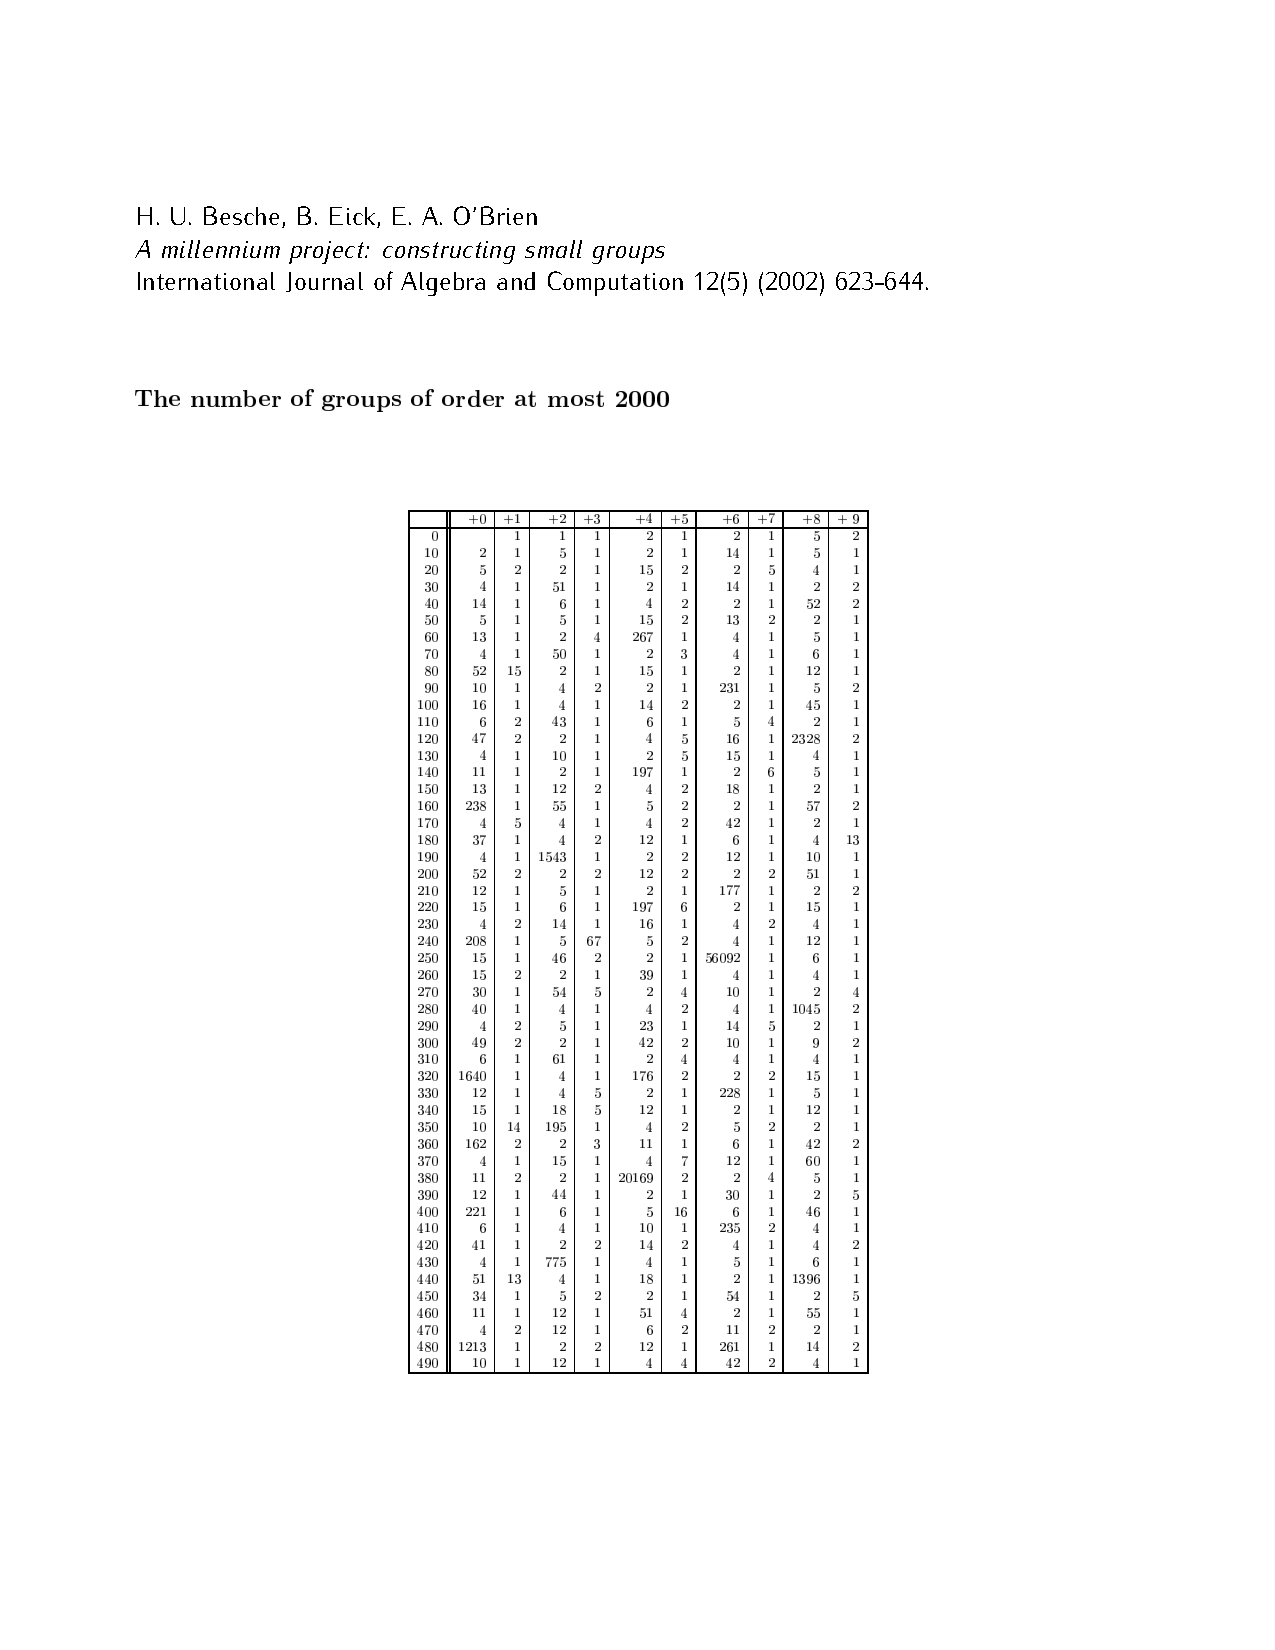
\includepdf[pages={1-4}]{pictures/small_group_table.pdf}






%%%%%%%%%%%%%%%%%%%%%%%%%%%%%%%
%%%%%%%%%%%%%%%%%%%%%%%%%%%%%%%
%%%
%%% GROUP EXTENSIONS AND COMPOSITION SERIES
%%%
%%%%%%%%%%%%%%%%%%%%%%%%%%%%%%%
%%%%%%%%%%%%%%%%%%%%%%%%%%%%%%%


\newpage
\section{Group extensions and composition series}
\label{SEC_GPEXTCOMPSERIES}



\begin{definition}
Let
$${\dots} \lra G_{i} \overset{f_{i}}{\lra} G_{i+1}  \overset{f_{i+1}}{\lra} G_{i+2} \lra {\dots}$$
be a sequence of groups and group homomorphisms. This sequence is \emph{exact}
if $\Im(f_{i}) = \Ker(f_{i+1})$ for all $i$. 
\end{definition}


\vs\vs

\begin{definition}
A \emph{short exact sequence} is an exact sequence of the form 
$$ 1\lra N \overset{f}{\lra} G \overset{g}{\lra} K \lra 1$$
(where $1$ is the trivial group).
\end{definition}

\vs\vs

\begin{note}\ 

\vskip -13mm

\ 
\benu
\item A sequence $1 \to N \overset{f}{\lra} G \overset{g}{\lra} K \to 1$ is a short exact sequence
iff 

\vskip -8mm

\ 
\bit
\item $f$ is a monomorphism 
\item $g$ is an epimorphism
\item $\Im(f) = \Ker(g)$.
\eit 

\item If $H\lhd G$ then we have a short exact sequence 
$$1 \lra H \lra G \lra G/H \lra 1$$
Morever,  up to an isomorphism, every short exact sequence is of this form:
$$
\xymatrix{
1 \ar[r] & N \ar[r]^{f}\ar[d]_{\cong} & G \ar[r]^{g}\ar[d]_{=} & K \ar[r]\ar[d]^{\cong} & 1 \\ 
1 \ar[r] & \Ker(g) \ar[r] & G \ar[r] & G/\Ker(g) \ar[r] & 1 \\ 
}
$$

\eenu

\end{note}


\vs\vs 

\begin{definition}
If a group $G$ fits into a short exact sequence 
$$ 1\lra N \overset{f}{\lra} G \overset{g}{\lra} K \lra 1$$
then we say that $G$ is an \emph{extension of $K$ by $N$}.
\end{definition}


\vs\vs

\begin{example}
For any $n>1$ the dihedral group $D_{n}$ and the cyclic group $\Z/2n\Z$ are 
non-isomorphic extensions of $\Z/n\Z$ by $\Z/2\Z$.
\end{example}


\vs\vs

\begin{definition}
A group $G$ is a \emph{simple group} if $G\neq \{e\}$ and the only normal subgroups of $G$
are $G$ and $\{e\}$.
\end{definition}

\vs

\begin{example}
$\Z/p\Z$ is a simple group for every prime $p$.
\end{example}


\textbf{Note.} A group $G$ is simple iff it is not a non-trivial extension of any  group. 



\vs\vs

\begin{definition}
If $G$ is a group then a \emph{normal series} of $G$ is a sequence of subgroups
$$\{e\} = G_{0} \subseteq G_{1} \subseteq G_{2} \subseteq {\dots}\subseteq G_{k} = G$$
such that $G_{i-1}\lhd G_{i}$ for all $i$.

A \emph{composition series} of $G$ is a normal series such that all quotient groups 
$G_{i}/G_{i-1}$ are simple.
\end{definition}

\vs\vs

\begin{example}
Take the dihedral group $D_{4} = \Z/4\Z \rtimes \Z/2\Z$.
We have a composition series
$$\{0\}\ \subseteq\  \Z/2\Z \ \subseteq\  \Z/4\Z \ \subseteq\  D_{4}$$

Another composition series of $D_{4}$: 
$$\{0\}\ \subseteq\  \Z/2\Z \ \subseteq\  \Z/2\Z  \times \Z/2\Z \ \subseteq\  D_{4}$$  

\end{example}


\vs\vs

\begin{theorem}[Jordan -- H\"{o}lder]
\label{THM_JORDANHOLDER}
If $G\neq \{e\}$ is a finite group then 

\vskip -11mm


\ 
\benu
\item $G$ has a composition series.
\item All composition series of $G$ are equivalent in the following sense. If 
we have composition series
$$\{e\}= G_{0} \subseteq {\dots} \subseteq G_{k} = G \ \ \ \ \ \text{and} \ \ \ \ \  
\{e\}= H_{0} \subseteq {\dots} \subseteq H_{l} = G$$
then $k=l$ and there is a bijection $\sigma \colon \{1, \dots, k\} \to \{1, \dots, k\}$
such that for  $i=1, \dots, k$ we have an isomorphism 
$$G_{i}/G_{i-1} \cong H_{\sigma(i)}/H_{\sigma(i)-1}$$
\eenu
 
\end{theorem}

\begin{proof}
Exercise (or see Hungerford p. 111).
\end{proof}


\vs\vs

\textbf{Upshot.} If $G\neq \{e\}$ is a finite group then $G$ can be obtained by 
taking successive extensions of simple groups as follows.

\vskip -13mm

\  
\benu 
\item Take a composition series 
$$\{e\} = G_{0} \subseteq G_{1} \subseteq G_{2} \subseteq {\dots}\subseteq G_{k} = G$$
\item For every $i=1, \dots, k$ we have a short exact sequence 
$$1 \lra G_{i-1} \lra G_{i} \lra G_{i}/G_{i-1} \lra 1$$ 
where $G_{i}/G_{i-1}$ is a simple group. Therefore 

$G_{1}$ is an extension of $G_{1}/G_{0}$ by $G_{0}$

\vskip -1mm
$G_{2}$ is an extension of $G_{2}/G_{1}$ by $G_{1}$ \newline
$\dots \ \ \ \ \  \ \dots  \ \ \ \ \ \    \dots \ \ \ \ \ \    \dots \ \ \ \ \ \  \dots$ \newline
$\dots \ \ \ \ \  \ \dots  \ \ \ \ \ \    \dots \ \ \ \ \ \    \dots \ \ \ \ \ \  \dots$

\vskip -1mm
$G= G_{k}$ is an extension of $G_{k}/G_{k-1}$ by $G_{k-1}$ \newline
\eenu



\newpage

\centerline{\textbf{The grand plan for classifying all finite groups (The H\"{o}lder Program)}}

\vskip -8mm

\ 
\benu
\item Classify all finite simple groups. 
\item For any two groups $N$, $K$ describe all possible extensions of $K$ by $N$.
\eenu

\textbf{Good news:} part 1) is done. See 

\href{http://www.ams.org/journals/bull/2001-38-03/S0273-0979-01-00909-0/S0273-0979-01-00909-0.pdf}
{
R. Solomon, \emph{A brief history of the classification of the finite simple groups}, 
Bulletin AMS 38 (3) (2001), 315-352.
}

\vskip -1mm

\href{http://www.ams.org/notices/200407/fea-aschbacher.pdf}
{
M. Aschbacher,  \emph{The status of the classification of the finite simple groups}, 
Notices AMS 51(7) (2004), 736-740.
}


%%%%%%%%%%%%%%%%%%%%%%%%%%%%%%%
%%%%%%%%%%%%%%%%%%%%%%%%%%%%%%%
%%%
%%% SIMPLE GROUPS
%%%
%%%%%%%%%%%%%%%%%%%%%%%%%%%%%%%
%%%%%%%%%%%%%%%%%%%%%%%%%%%%%%%


\newpage
\section{Simple groups}
\label{SEC_SIMPLEGPS}


\textbf{Recall.} A group $G\neq\{e\}$ is a simple group if  the only normal subgroups 
of $G$ are $G$ and $\{e\}$.

\vs

\textbf{Note.} If $G$ is a simple group then any non-trivial homomorphism $f\colon G\to H$
is a monomorphism. 

\vs\vs

\begin{proposition}
If $G$ is an abelian group then $G$ is simple iff $G\cong \Z/p\Z$ for some prime $p$.
\end{proposition}



\begin{proof}
Exercise.
\end{proof}



\vs\vs

\begin{proposition}
\label{PROP_SIMPLEPGP}
If $G$ is a simple $p$-group then $G\cong \Z/p\Z$.
\end{proposition}

\begin{proof}
If $G$ is a $p$-group then $Z(G) \neq \{e\}$ by (\ref {THM_NONTRIVPCENTER}). 
We have $Z(G) \lhd G$, so if $G$ is simple we must have $G = Z(G)$. Therefore 
$G$ is a simple abelian $p$-group, and so $G\cong \Z/p\Z$.  
\end{proof}

\vs\vs

\begin{lemma}
\label{LEMMA_SIMPLEPRMGP}
There are no non-abelian simple groups of order $p^{r}m$ where $p$ is a prime, 
$r\geq 1$, $p\nmid m$ and $p^{r}m \nmid m!$.
\end{lemma}


\vs

\begin{proof}
Assume that $G$ is a simple, non-abelian group of such order. We must have $m > 1$
(since if $m=1$ then $G$ is a $p$-group). Let $P$ be a Sylow $p$-subgroup of $G$. 
Consider the action of $G$ on the left cosets $G/P$:
$$G\times G/P \to G/P, \ \ \ \ \ a\cdot bP = (ab)P$$ 
This action defines a homomorphism 
$$\varrho \colon G \to \Perm(G/P)$$ 
where $\Perm(G/P)$ is the group of all permutations of the set 
$G/P$. Since $G\neq P$ this homomorphism is non-trivial, and so, since $G$ is a simple group, 
$\varrho$ is a monomorphism. Therefore $G$ can be identified with a subgroup of 
$\Perm(G/P)$. By Lagrange's Theorem (\ref{THM_LAGRANGE}) we obtain that 
$|G|$ divides $|\Perm(G/P)|$. Since $|\Perm(G/P)| = m!$ this gives 
$$p^{r}m \mid m!$$
which contradicts assumptions of the lemma. 
\end{proof}


\vs\vs


\begin{theorem}
\label{THM_SIMPLEGPSLESS60}
There are no non-abelian simple groups of order  $<60$.
\end{theorem}

\vs

\begin{proof}
Check: If $1\leq n < 60$, and $n\neq 30, 40, 56$ then $n$ is of the form $p^{r}m$
for some prime $p$, and $r, m \geq 1$ such that $p\nmid m$ and $p^{r}m \nmid m!$. 

By Lemma \ref{LEMMA_SIMPLEPRMGP}   we obtain then that a non-abelian group $G$  
of order $n< 60$ may be simple only if $n=30, 40$ and $56$. 

Assume that $|G| = 30 = 2\cdot 3 \cdot 5$. We will show that $G$ cannot be a simple group.

We argue by contradiction. Assume that $G$ is simple and 
let $s_{3}$ be the number of Sylow $3$-subgroups of $G$. We have
$$s_{3} \mid 10 \ \ \ \text{and} \ \ \ s_{3} \equiv 1 \ (\mathrm{mod} \ 3)$$
It follows that either $s_{3} = 1$ or $s_{3}=10$. Since $G$ is simple $s_{3}\neq 1$, so 
$s_{3} = 10$. 

Notice that if $P$, $P'$ are two distinct Sylow $3$-subgroups of $G$ then $P\cap P' = \{e\}$. 
We obtain:

\vskip -13mm

\ 
\bit
\isep
\item[--] $G$ contains $10$ Sylow $3$-subgroups. 
\item[--] each Sylow $3$-subgroup contains $2$ elements of order $3$.
\eit
 
It follows that $G$ contains $20$ elements of order $3$. 

By a similar argument we obtain that 
\vskip -13mm

\ 
\bit
\isep
\item[--] $G$ must contain $6$ Sylow $5$-subgroups. 
\item[--] each Sylow $5$-subgroup contains $4$ elements of order $3$.
\eit
so we have $24$ elements of order $5$ in $G$. 
This is however impossible, since $20 + 24  > 30 = |G|$.



In a similar way one can show that if $|G| = 40$ or $|G|=56$ then $G$ is not
a simple group (exercise)
\end{proof}


\textbf{Next goal:} there are infinitely many  non-abelian simple finite groups. 
In particular there is a simple group of order $60$. 




%%%%%%%%%%%%%%%%%%%%%%%%%%%%%%%
%%%%%%%%%%%%%%%%%%%%%%%%%%%%%%%
%%%
%%% SYMMETRIC AND ALTERNATING GROUPS
%%%
%%%%%%%%%%%%%%%%%%%%%%%%%%%%%%%
%%%%%%%%%%%%%%%%%%%%%%%%%%%%%%%


\newpage
\section{Symmetric and alternating groups}
\label{SEC_SYMALTGPS}


\textbf{Recall.} The symmetric group on $n$ letters is the group 
$$S_{n} = \Perm(\{1, \dots, n\})$$


\vs\vs


\begin{theorem}[Cayley]
If $G$ is a group of order $n$ then $G$ is isomorphic to a subgroup of $S_{n}$.
\end{theorem}

\vs 

\begin{proof}
Let $S$ be the set of all elements of $G$. Consider the action of $G$ on $S$
$$G \times S \to S, \ \ \ a\cdot b := ab$$
This action defines a homomorphism $\varrho \colon G \to \Perm(S)$. Check: this homomorphism 
is 1-1. It follows that $G$ is isomorphic to a subgroup of $\Perm(S)$. Finally, since $|S| = n$ 
we have $\Perm(S) \cong S_{n}$.
\end{proof}



\vs\vs

\begin{notation}
Denote 
$$[n] := \{1, \dots, n\}$$
If $\sigma \in S_{n}$, $\sigma\colon [n] \to [n]$ then we write
$$\sigma = 
\begin{pmatrix}
1 & 2 & 3 & \dots & n \\[2mm]
\sigma(1) & \sigma(2) & \sigma(3) & \dots & \sigma(n) \\
\end{pmatrix}
$$
\end{notation}

\vs\vs

\begin{definition}
A permutation $\sigma\in S_{n}$ is a \emph{cycle of length $r$} (or \emph{$r$-cycle}) if there are distinct integers 
$i_{1}, \dots, i_{r}\in [n]$ such that 
$$\sigma(i_{1}) = i_{2}, \ \sigma(i_{2}) = i_{3}, \ \dots\ , \ \sigma(i_{r}) = i_{1}$$
and $\sigma(j) = j$ for $j\neq i_{1}, \dots, i_{r}$.

A cycle of length 2 is called a \emph{transposition}. 
\end{definition}

\vs

\textbf{Note.} The only cycle of length 1 is the identity element in $S_{n}$.


\vs\vs

\begin{notation}
If $\sigma$ is a cycle as above then we write
$$\sigma = (i_{1} \  i_{2} \  \dots \  i_{r})$$

\end{notation}

\vs\vs

\begin{example}
In $S_{5}$ we have 
$$
\begin{pmatrix}
1 & 2 & 3 & 4 & 5 \\[2mm]
1 & 4 & 2 & 5 & 3 \\
\end{pmatrix}
= (2 \ 4\ 5\ 3)
$$
Note: $ (2 \ 4\ 5\ 3) =  (4\ 5\ 3\ 2) = (5\ 3\ 2\ 4) = (3\ 2\ 4\ 5)$.
\end{example}

\vs\vs

\begin{definition}
Permutations $\sigma, \tau\in S_{n}$ are \emph{disjoint} if 
$$\{i\in [n] \ | \  \sigma(i) \neq i \} \ \cap\  \{j\in [n] \ | \ \tau(j) \neq j \} = \varnothing$$
\end{definition}

\vs\vs

\begin{proposition}
If $\sigma, \tau$ are disjoint permutations then $\sigma\tau = \tau\sigma$.
\end{proposition}

\begin{proof}
Exercise.
\end{proof}


\vs\vs


\begin{proposition}
\label{PROP_CYCLEDECOMP}
Every non-identity permutation $\sigma\in S_{n}$ is a product of disjoint cycles of length $\geq 2$.
Moreover, this decomposition into cycles is unique up to the order of factors.  
\end{proposition}

\vs\vs

\begin{example}
Let $\sigma\in S_{9}$
$$
\sigma = 
\begin{pmatrix}
1 & 2 & 3 & 4 & 5 & 6 & 7 & 8 & 9\\[2mm]
4 & 7 & 1 & 3 & 2 & 6 & 5 &  9 & 8\\
\end{pmatrix}
$$
Then $\sigma = (1 \ 4\ 3)(2\ 7\ 5)(8\ 9)$.
\end{example}


\vs\vs

\begin{proof}[Proof of proposition \ref{PROP_CYCLEDECOMP}.]
Consider the action of $\Z$ on the set $[n]$ given by 
$$k\cdot i = \sigma^{k}(i)$$
for $k\in \Z$, $i\in [n]$. Notice that 
$$\Orb(i) = \{ \sigma^{k}(i) \ \mid \  k\in \Z \}$$
Define $\sigma_{i}\colon [n] \to [n]$
$$
\sigma_{i}(j)  = 
\begin{cases}
 \ \sigma(j) & \text{if } j\in \Orb(i)  \\
\ j & \text{otherwise} 
\end{cases}
$$
Notice that $\sigma_{i}$ is a bijection since $\sigma(\Orb(i)) = \Orb(i)$. Thus $\sigma_{i}\in S_{n}$. 
Check: 

\vskip -13mm

\ 
\benu
\item $\sigma_{i}$ is a cycle of length $|\Orb(i)|$.
\item if $\Orb(i_{1}), \dots, \Orb(i_{r})$ are all distinct orbits of $[n]$ containing more 
than one element then $\sigma_{i_{1}}, \dots, \sigma_{i_{r}}$ are non-trivial, disjoint cycles and 
$$\sigma = \sigma_{i_{1}}\cdot {\dots}\cdot \sigma_{i_{r}}$$
\eenu
Uniqueness of decomposition - easy. 
\end{proof}

\vs\vs


\begin{proposition}
\label{PROP_TRANSPPROD}
Every permutation $\sigma\in S_{n}$ is a product of (not necessarily disjoint)  transpositions.
\end{proposition}


\vs

\begin{proof}
By Proposition \ref{PROP_CYCLEDECOMP} it is enough to show that every cycle is 
a product of transpositions. We have:
$$(i_{1} \ i_{2} \ i_{3} \ \dots \ i_{r}) = (i_{1} \ i_{r})(i_{1}\ i_{r-1})\cdot {\dots}\cdot (i_{1}\ i_{3})(i_{1}\ i_{2})$$ 
\end{proof}


\vs


\textbf{Note.} For $\sigma\in S_{n}$ we have a bijection
$$\sigma\times\sigma\colon [n]\times [n]\to [n]\times[n]$$
given by $\sigma\times\sigma(i, j) = (\sigma(i), \sigma(j))$.
Define
$$S_{\sigma} := \{ (i, j) \in [n]\times [n] \ \mid \ i> j \text{ and } \sigma(i) < \sigma(j) \}$$


\vs\vs

\begin{definition}
A permutation $\sigma\in S_{n}$ is \emph{even} (resp. \emph{odd}) if the number of elements 
of $S_{\sigma}$ is even (resp. odd).
\end{definition}

\vs\vs

\begin{theorem}
\label{THM_PERMSIGN}

1) The map $\sgn\colon S_{n}\to \Z/2\Z$ defined by 
$$
\sgn(\sigma) = 
\begin{cases}
0 & \text{if $\sigma$ is even} \\
1 & \text{if $\sigma$ is odd}
\end{cases}
$$
is a homomorphism. 

2) If $\sigma$ is a transposition then $\sgn(\sigma) =1$, 
so this homomorphism is non-trivial.
\end{theorem}

\vs

\begin{proof}
1) Let $\sigma, \tau\in S_{n}$. Denote $s_{\sigma} = |S_{\sigma}|$. 
We want to show
$$s_{\tau\sigma} \equiv s_{\tau} + s_{\sigma} \ (\mathrm{mod} \ 2) $$

Let $[n]^{+} := \{ (i, j) \in [n]\times [n] \ \mid \ i> j \}$. Define subsets
$P_{\sigma}, R_{\sigma}, P_{\tau}, R_{\tau}\subseteq [n]^{+}$ as follows:
\begin{align*}
P_{\sigma} :=  & \{(i, j) \ \mid \ \sigma^{-1}(i) > \sigma^{-1}(j)\} \\
R_{\sigma} :=  & \{(i, j) \ \mid \ \sigma^{-1}(i) < \sigma^{-1}(j)\} \\
P_{\tau} :=  & \{(i, j) \ \mid \ \tau(i) > \tau(j)\} \\
R_{\tau} :=  & \{(i, j) \ \mid \ \tau(i) < \tau(j)\} \\
\end{align*}
Notice that $s_{\sigma} = |R_{\sigma}|$ and $s_{\tau} = |R_{\tau}|$. Notice also 
that $(i, j)\in S_{\tau\sigma}$ iff either $(\tau(i), \tau(j)) \in P_{\sigma}\cap R_{\tau}$
or $(\tau(j), \tau(i)) \in R_{\sigma} \cap P_{\tau}$. This gives
$$s_{\tau\sigma} = |P_{\sigma}\cap R_{\tau}| + | R_{\sigma} \cap P_{\tau}|$$
On the other hand we have:
$$s_{\sigma} = |R_{\sigma}| = |R_{\sigma}\cap P_{\tau}| + |R_{\sigma}\cap R_{\tau}|$$
$$s_{\tau} = |R_{\tau}| = |P_{\sigma}\cap R_{\tau}| + |R_{\sigma}\cap R_{\tau}|$$
Therefore 
$$s_{\sigma} + s_{\tau} =  |R_{\sigma}\cap P_{\tau}| +  |P_{\sigma}\cap R_{\tau}| + 
2|R_{\sigma}\cap R_{\tau}| = s_{\tau\sigma} + 2|R_{\sigma}\cap R_{\tau}|$$
and so  $s_{\tau} + s_{\sigma} \equiv  s_{\tau\sigma} \ (\mathrm{mod} \ 2) $.

\vs

2) Exercise.
\end{proof}




\vs\vs\vs

\begin{definition/proposition}
The set 
$$A_{n} = \{ \sigma \in S_{n} \ | \ \sigma \text{ is even} \}$$
is a normal subgroup of $S_{n}$. It is called the 
\emph{alternating group on $n$ letters}.
\end{definition/proposition}

\vs

\begin{proof}
It is enough to notice that $A_{n} = \Ker(\sgn)$.
\end{proof}


\vs\vs

\textbf{Note.} We have 
$$S_{n}/A_{n} \cong \Z/2\Z$$ 
Since $|S_{n}| = n!$ thus $|A_{n}| = \frac{n!}{2}$.


\vs\vs

\begin{proposition}
If $\sigma\in S_{n}$ then $\sigma$ is even (resp. odd) iff $\sigma$ is a product 
of an even (resp. odd) number of transpositions. 
\end{proposition}

\vs

\begin{proof}
If $\sigma = \tau_{1}{\dots}\tau_{m}$ where $\tau_{1}, \dots, \tau_{m}$
are transpositions then 
$$\sgn(\sigma) = \sgn( \tau_{1}{\dots}\tau_{m}) = \sum_{i=1}^{m}\sgn(\tau_{i}) = \sum_{i=1}^{m}1$$
Thus $\sgn(\sigma) = 0$ iff $m$ is even and $\sgn(\sigma) = 1$ iff $m$ is odd.

\end{proof}


\vs\vs

\textbf{Note.} If follows that if a permutation $\sigma\in S_{n}$ is a product of an even 
number of transpositions then it cannot be written as a product of an odd number of transpositions
(and vice versa). 

\vs\vs

\begin{corollary}
A permutation $\sigma\in S_{n}$ is even iff
$$\sigma= \sigma_{1}\sigma_{2}{\dots}\sigma_{r}$$ 
where $\sigma_{i}$ is a cycle of length $m_{i}$ and  $\sum_{i=1}^{r}(m_{i} -1) $ is even.
\end{corollary}

\vs

\begin{proof} \ 
It is enough to notice that by the proof of Proposition \ref{PROP_TRANSPPROD} a cycle
of length $m$ is a product of $m-1$ transpositions.  
\end{proof}


\vs

\textbf{Note.} The usual notation for the sign of a permutation is
$$
\sgn(\sigma) = 
\begin{cases}
\phantom{-}1 & \text{if $\sigma$ is even} \\
 -1 & \text{if $\sigma$ is odd}
\end{cases}
$$
where $\{-1, 1\} \cong \Z/2\Z$ is the multiplicative group of units in $\Z$.



%%%%%%%%%%%%%%%%%%%%%%%%%%%%%%%
%%%%%%%%%%%%%%%%%%%%%%%%%%%%%%%
%%%
%%% SIMPLICITY OF ALTERNATING GROUPS
%%%
%%%%%%%%%%%%%%%%%%%%%%%%%%%%%%%
%%%%%%%%%%%%%%%%%%%%%%%%%%%%%%%


\newpage
\section{Simplicity of  alternating groups}
\label{SEC_SIMPALTGPS}


\begin{theorem}
\label{THM_ALTSIMP}
The alternating group $A_{n}$ is simple for  $n \geq 5$.
\end{theorem}

\vs\vs

\begin{lemma}
\label{LEMMA_ANSIMPL1}
For $n\geq 3$   every element of $A_{n}$ is a product of 3-cycles. 
\end{lemma}

\vs

\begin{proof}
It is enough to show that if $n\geq 3$ and  $\tau$, $\sigma$ are transpositions in $S_{n}$
then $\tau\sigma$ is a product of 3-cycles. 

Case 1) \ $\tau$, $\sigma$ are disjoint transpositions: $\tau = (i \ j)$, $\sigma = (k \ l)$ for 
distinct elements $i, j, k, l \in [n]$. Then we have
$$\tau\sigma = (i \ j \ k)(j \ k \ l)$$


Case 2) \ $\tau$, $\sigma$ are not disjoint: $\tau = (i \ j)$, $\sigma = (j \ k)$. Then 
$$\tau\sigma = (i\ j \ k)$$

\end{proof}

\vs\vs

\begin{lemma}
\label{LEMMA_ANSIMPL2}
If $n\geq 5$ and $\sigma$, $\sigma'$ are 3-cycles  in $S_{n}$ then 
$$\sigma' = \tau\sigma\tau^{-1}$$
for some $\tau\in A_{n}$
\end{lemma}

\vs

\begin{proof}
Check: if $(i_{1} \ i_{2} \ \dots \ i_{r})$ is a cycle in $S_{n}$ then for any 
$\omega\in S_{n}$ we have 
$$\omega(i_{1} \ i_{2} \ \dots \ i_{r})\omega^{-1} = (\omega(i_{1}) \ \omega(i_{2}) \ \dots \omega(\ i_{r}))$$
If $\sigma  = (i_{1} \ i_{2} \ i_{3})$, $\sigma' = (j_{1}\ j_{2}\ j_{3})$ then take $\omega\in S_{n}$
such that $\omega(i_{k}) = j_{k}$ for $k=1, 2, 3$. We have
$$\sigma' = \omega \sigma \omega^{-1}$$
If $\omega\in A_{n}$ we can then take $\tau := \omega$.

Assume then that $\omega\not\in A_{n}$. 
Since $n\geq 5$ there are $r, s\in [n]$ such that $(r \ s)$ and $\sigma = (i_{1} \  i_{2}\ i_{3})$
are disjoint cycles. Take $\tau = \omega (r\ s)$.  Then $\tau \in A_{n}$. Moreover, since 
$(r\ s)$ commutes with $\sigma$ we have
$$\tau\sigma\tau^{-1} =  \omega (r\ s)\sigma(r\ s)^{-1} \omega^{-1} = \omega \sigma \omega^{-1} = \sigma'$$
\end{proof}


\vs\vs

\begin{corollary}
\label{COR_SIMPLE3CYCLE}
If $n\geq 5$ and $H$ is a normal subgroup of $A_{n}$ such that $H$ contains some 3-cycle 
then $H = A_{n}$.
\end{corollary}

\vs

\begin{proof}
By Lemma \ref{LEMMA_ANSIMPL2} $H$  contains all 3-cycles, and so by 
Lemma \ref{LEMMA_ANSIMPL1} it contains all elements of $A_{n}$.
\end{proof}


\vs\vs

\begin{proof}[Proof of Theorem \ref{THM_ALTSIMP}]
Let $n\geq 5$, $H\lhd A_{n}$ and $H \neq \{(1)\}$. We need to show that $H= A_{n}$.
By Corollary \ref{COR_SIMPLE3CYCLE} it will suffice to show that $H$ contains 
some 3-cycle.

Let $(1)\neq \sigma$ be an element of $H$ with the maximal number of fixed points in $[n]$.
We will show that $\sigma$ is 3-cycle. Take the decompositon of $\sigma$ into dosjoint 
cycles:
$$\sigma = \sigma_{1}\sigma_{2}\cdot {\dots}\cdot \sigma_{m}$$

Case 1) \ $\sigma_{1}, \dots, \sigma_{m}$ are transpositions. 

Since $\sigma\in A_{n}$ we must then have $m\geq 2$. Say,  $\sigma_{1} = (i\ j)$, $\sigma_{2} = (k\ l)$. 
Take $s\neq i, j, k, l$ and let $\tau=(k\ l\ s)\in A_{n}$. Since $H$ is normal in $A_{n}$ we have 
$$\tau\sigma\tau^{-1}\sigma^{-1} \in H$$ 
Check:


\vskip -13mm

\ 
\benu
\isep
\item  $\tau\sigma\tau^{-1}\sigma^{-1} \neq (1)$ since $\tau\sigma\tau^{-1}\sigma^{-1}(k)\neq k$
\item  $\tau\sigma\tau^{-1}\sigma^{-1}$ fixes every element of $[n]$ fixed by $\sigma$
\item $\tau\sigma\tau^{-1}\sigma^{-1}$ fixes $i, j$.
\eenu
 
 Thus $\tau\sigma\tau^{-1}\sigma^{-1}$ has more fixed points than $\sigma$ which is impossible 
 by the definition of $\sigma$.

\vs

Case 2) \ $\sigma_{r} $ is a cycle of length $\geq 3$ for some $1\leq r \leq m$. 

We can assume $r=1$: $\sigma_{1} = (i\ j\ k \dots)$. If $\sigma = \sigma_{1}$ and $\sigma_{1}$
is a 3-cycle we are done. 

Otherwise $\sigma$ must move at least two more elements, say $p, q$. In such case take $\tau= (k \ p \ q)$. We have  
$$\tau\sigma\tau^{-1}\sigma^{-1}  \in H$$
 Check:


\vskip -13mm

\ 
\benu
\isep
\item  $\tau\sigma\tau^{-1}\sigma^{-1} \neq (1)$ since $\tau\sigma\tau^{-1}\sigma^{-1}(k)\neq k$
\item  $\tau\sigma\tau^{-1}\sigma^{-1}$ fixes every element of $[n]$ fixed by $\sigma$
\item $\tau\sigma\tau^{-1}\sigma^{-1}$ fixes $j$.
\eenu

 Thus $\tau\sigma\tau^{-1}\sigma^{-1}$ has more fixed points than $\sigma$ which is again impossible 
 by the definition of $\sigma$.
 
 As a consequence $\sigma$ must be a 3-cycle. 
 
\end{proof}


\vs



\begin{nn} \textbf{Classification of simple finite groups.}

\vskip -13mm

\ 
\benu
\isep
\item cyclic groups $\Z/p\Z$, $p$ -- prime
\item alternating groups $A_{n}$, $n\geq 5$ 
\item finite simple groups of Lie type, e.g. projective special linear groups
$$PSL_{n}(\F) := SL_{n}(\F)/Z(SL_{n}(\F))$$
$\F$ -finite field, $n\geq 2$ (and $n>2$ if $\F = \F_{2}$ or $\F = \F_{3}$).
\item 26 sporadic groups (the smallest: Mathieu group $M_{11}$, $|M_{11}| =7920$, 
the biggest: the Monster $M$, $|M|\approx 8\cdot 10^{53}$).
\eenu

\end{nn}



%%%%%%%%%%%%%%%%%%%%%%%%%%%%%%%
%%%%%%%%%%%%%%%%%%%%%%%%%%%%%%%
%%%
%%% SOLVABLE  GROUPS
%%%
%%%%%%%%%%%%%%%%%%%%%%%%%%%%%%%
%%%%%%%%%%%%%%%%%%%%%%%%%%%%%%%


\newpage
\section{Solvable groups}
\label{SEC_SOLVGPS}

\textbf{Recall.} Every finite group $G$ has a composition series:
$$\{e\}= G_{0} \subseteq {\dots} \subseteq G_{k} = G$$
where $G_{i-1}\lhd G_{i}$ and $G_{i}/G_{i-1}$ is a simple group. 

\vs\vs


\begin{definition}
A group $G$ is \emph{solvable} if it has a composition series
$$\{e\}= G_{0} \subseteq {\dots} \subseteq G_{k} = G$$
such that for every $i$ the group $G_{i}/G_{i-1}$ is a simple abelian group
(i.e. $G_{i}/G_{i-1}\cong \Z/p_{i}\Z$ for some prime $p_{i}$). 
\end{definition}


\vs\vs

\begin{example}\ 

\vskip -13mm 

\ 
\benu
\item Every finite abelian group is solvable. 
\item For $n\geq 5$ the symmetric group $S_{n}$ has a  composition series 
$$\{(1)\} \subseteq A_{n} \subseteq S_{n}$$
and so $S_{n}$ is not solvable. 
\eenu

\end{example}


\vs\vs

\begin{proposition}
A finite group $G$ is solvable iff it has a normal series 
$$\{e\}= H_{0} \subseteq {\dots} \subseteq H_{l} = G$$
such that $H_{j}/H_{j-1}$ is an abelian group for all $j$.
\end{proposition}

\begin{proof}
Exercise. 
\end{proof}


\newpage

\textbf{Recall.} 

\vskip -13mm
\ 
\benu
\item If $G$ is a group the $[G, G]$ is the commutator subgroup of $G$
$$[G, G] = \subgp{\{aba^{-1}b^{-1} \ \mid \ a, b\in G \}}$$
\item $[G, G]$ is the smallest normal subgroup of $G$ such that $G/[G, G]$ is abelian:
if $G/H$ for some $H\lhd G$ then $[G, G]\subseteq H$.
 \eenu

\vs\vs

\begin{definition}
For a group $G$ the \emph{derived series of $G$} is the normal series
$$\dots \subseteq G^{(2)}\subseteq G^{(1)}\subseteq G^{(0)} =  G$$
where  $G^{i+1} = [G^{(i)}, G^{(i)}]$ for $i\geq 1$. The group $G^{(i)}$ is called 
the \emph{$i$-th derived group of $G$}.
\end{definition}

\vs\vs

\begin{theorem}
A group $G$ is solvable iff $G^{(n)} = \{e\}$ for some $n\geq 0$.
\end{theorem}

\vs

\begin{proof}
Exercise. 
\end{proof}

\vs\vs

\begin{theorem}\ 
\label{THM_SOLVGPSSUBQUOTEXT}

\vskip -13mm

\ 
\benu
\isep
\item Every subgroup of a solvable group is solvable.
\item Ever quotient group of a solvable group is solvable.
\item If $H\lhd G$, and both $H$ and  $G/H$ are solvable groups then  $G$ is also solvable.
\eenu

\end{theorem}


\vs

\begin{proof} \ 

1) If  $H\subseteq G$ then $H^{(i)} \subseteq G^{(i)}$. Thus
if $G^{(n)} = \{e\}$ then $H^{(n)} = \{e\}$.

\vs

2) For $H\lhd G$ take the canonical epimorphism $f\colon G \to G/H$. 
We have 
$$f(G^{(i)}) = (G/H)^{(i)}$$
Therefore if $G^{(n)} =\{e\}$ then $(G/H)^{(n)} = \{e\}$.

\vs

3) Assume that $H\lhd G$, and that $H^{(m)}$, $(G/H)^{(n)}$ are trivial groups. Consider the  
canonical epimorphism $f\colon G \to G/H$. We have 
$$f(G^{(n)}) = (G/H)^{(n)} = \{e\}$$
Therefore $G^{(n)}\subseteq \Ker(f) = H$. As a consequence we obtain
$$G^{(n+m)} = \left(G^{(n)}\right)^{(m)} \subseteq H^{(m)} = \{ e\}$$
 
 \end{proof}

 

\vs\vs

\begin{theorem}[Feit-Thompson]
\label{THM_FEITTHOMPSON}
Every finite group of odd order is solvable. 
\end{theorem}

\begin{proof}
See:
W. Feit, J.G. Thompson, \emph{Solvability of groups of odd order}, 
 Pacific Journal of Mathematics 13(3) (1963), 775-1029.

\end{proof}

\vs\vs


\begin{corollary}
There are no non-abelian finite simple groups of odd order.  
\end{corollary}

\vs

\begin{proof}
Let $G\neq \{e\}$ be a simple group of odd order. By Theorem \ref{THM_FEITTHOMPSON}
$G$ is solvable so $[G, G]\neq G$. Since $[G, G]\lhd G$, by simplicity of $G$ we must 
have $[G, G] = \{e\}$, and so $G$ is an abelian group. 
\end{proof}


%%%%%%%%%%%%%%%%%%%%%%%%%%%%%%%
%%%%%%%%%%%%%%%%%%%%%%%%%%%%%%%
%%%
%%% NILPOTENT GROUPS
%%%
%%%%%%%%%%%%%%%%%%%%%%%%%%%%%%%
%%%%%%%%%%%%%%%%%%%%%%%%%%%%%%%


\newpage
\section{Nilpotent groups}
\label{SEC_NILPGPS}


\begin{nn} Recall that if $G$ is a group then 
$$Z(G) = \{ a\in G \ \mid \  ab=ba \text{ for all } b\in G \}$$
Note that $Z(G)\lhd G$. Take the canonical epimorphism  $\pi\colon G \to G/ Z(G)$. 
Since $Z\left( G/Z(G)\right)\lhd G/Z(G)$ we have:
 $$\pi^{-1}\left(Z\left( G/Z(G)\right)\right) \lhd G$$
Define:

\vskip -13mm

\ 
\begin{align*}
Z_{1}(G) := & Z(G) \\
Z_{i}(G) :=  & \pi_{i}^{-1}\left(Z\left( G/Z_{i-1}(G)\right)\right) \ \ \  \ \text{ for } i>1
\end{align*}
where $\pi_{i}\colon G \to G/Z_{i-1}(G)$. We have $Z_{i}(G)\lhd G$ for all $i$.
\end{nn}


\vs\vs

\begin{definition}
The \emph{upper central series} of a group $G$ is a sequence of normal subgroups of $G$:
$$\{ e \} = Z_{0}(G) \subseteq Z_{1}(G) \subseteq Z_{2}(G) \subseteq \dots $$
\end{definition}


\vs\vs

\begin{definition}
A group $G$ is \emph{nilpotent}  if $Z_{i}(G) = G$ for some $i$.

If $G$ is a nilpotent group then the \emph{nilpotency class} of $G$ is the smallest
$n\geq 0$ such that $Z_{n}(G) = G$.
 \end{definition}

\vs\vs



\begin{proposition}
Every nilpotent  group is solvable.  
\end{proposition}


\begin{proof}
If $G$ is nilpotent group then the upper central series of $G$
$$\{ e \} = Z_{0}(G) \subseteq Z_{1}(G) \subseteq\  \dots \ \subseteq Z_{n}(G) = G $$
is a normal series. 

Moreover, for every $i$ we have
$$Z_{i}(G)/Z_{i-1}(G) = Z(G/Z_{i-1}(G))$$ 
so all quotients of the upper central series are abelian. 
\end{proof}

\vs\vs

\begin{note}
\label{NOTE_SOLVABLE_NOT_NILPOTENT}
Not every solvable group is nilpotent. Take e.g. $G_{T}$. We have $Z(G_{T}) = \{I\}$, and so 
$$Z_{i}(G_{T}) = \{I \}$$
for all $i$. Thus $G_{T}$ is not nilpotent. On the other hand $G_{T}$ is solvable with a composition series 
$$\{I\} \subseteq \{I, R_{1}, R_{2}\} \subseteq G_{T}$$
\end{note}


\vs\vs

\begin{proposition}\ 
\label{PROP_ABPGPNILP}

\vskip -13mm 


\ 
\benu
\isep[-1]
\item Every abelian group is nilpotent. 
\item Every finite  $p$-group is nilpotent. 
\eenu
\end{proposition}

\vs

\begin{proof}\ 

1)  If $G$ is abelian then $Z_{1}(G) = G$. 

2) If $G$ is a $p$-group then  so is $G/Z_{i}(G)$ for every $i$. By Theorem \ref{THM_NONTRIVPCENTER}
if $G/Z_{i}(G)$ is non-trivial then its center $Z(G/Z_{i}(G))$ a non-trivial group. 
This means  that if $Z_{i}(G)\neq G$ then $Z_{i}(G) \subseteq Z_{i+1}(G)$ and $Z_{i}(G)\neq Z_{i+1}(G)$. 
Since $G$ is finite we must have $Z_{n}(G) = G$ for some $G$.
\end{proof}


\vs\vs

\begin{definition}
A \emph{central series} of a group $G$ is a normal series 
$$\{e\}= G_{0} \subseteq {\dots} \subseteq G_{k} = G$$
such $G_{i}\lhd G$ and $G_{i+1}/G_{i}\subseteq Z(G/G_{i})$ for all $i$.
\end{definition}

\vs\vs

\begin{proposition}
If $\{e\}= G_{0} \subseteq {\dots} \subseteq G_{k} = G$ is a central series of $G$ then  
$$G_{i} \subseteq Z_{i}(G)$$
\end{proposition}

\vs

\begin{proof}
Exercise.
\end{proof}


\vs\vs

\begin{corollary}
\label{COR_CENTRSERIES}
A group $G$ is nilpotent iff it has a central series. 
\end{corollary}

\vs

\begin{proof}
If $G$ is nilpotent then 
$$\{ e \} = Z_{0}(G) \subseteq Z_{1}(G) \subseteq\  \dots \ \subseteq Z_{n}(G) = G $$
is a central series of $G$. 

Conversely, if 
$$\{e\}= G_{0} \subseteq {\dots} \subseteq G_{k} = G$$
is a central series of $G$ then by (\ref{COR_CENTRSERIES}) we have $G = G_{k} \subseteq Z_{k}(G)$, 
so $G = Z_{k}(G)$, and so 
$G$ is nilpotent.
\end{proof}

\vs\vs

\begin{note}
Given a group $G$ define
\begin{align*}
\Gamma_{0}(G) := & G \\
\Gamma_{i}(G) := & [G, \Gamma_{i-1}(G)] \ \ \  \text{ for $i>0$}.\\
\end{align*} 
We have  
$$ {\dots}  \subseteq \Gamma_{1}(G) \subseteq \Gamma_{0}(G) = G $$
\end{note}


\vs\vs

\begin{proposition} If $G$ is a group then
\vskip -13mm

\ 
\benu
\isep
\item $\Gamma_{i}(G) \lhd G$ for all $i$ 
\item $\Gamma_{i}(G)/\Gamma_{i+1}(G) \subseteq Z(G/\Gamma_{i+1}(G))$ for all $i$
\eenu
\end{proposition}

\vs

\begin{proof}
Exercise.
\end{proof}

\vs\vs

\begin{definition}
If $\Gamma_{n}(G) = \{e\}$ then 
$$\{e\} = \Gamma_{n}(G) \subseteq {\dots} \subseteq \Gamma_{0}(G) = G$$
is a central series of $G$. It is called the \emph{lower central series} of $G$.
\end{definition}

\vs\vs

\begin{proposition}
\label{PROP_LOCENTRALNIL}
A group $G$ is nilpotent iff $\Gamma_{n}(G) = \{e\}$
\end{proposition}


\begin{proof}
Exercise.
\end{proof}

\vs\vs


\begin{theorem}\ 
\label{THM_NILPGPSSUBQUOTEXT}
\vskip -13mm

\ 
\benu
\isep
\item Every subgroup of a nilpotent  group is nilpotent.
\item Ever quotient group of a nilpotent group is nilpotent.
\eenu
\end{theorem}

\vs

\begin{proof}
Exercise. 
\end{proof}


\vs\vs

\begin{note}
The properties of nilpotent group given  in Theorem \ref{THM_NILPGPSSUBQUOTEXT} are analogous to the first two properties of solvable groups from Theorem \ref{THM_SOLVGPSSUBQUOTEXT}. 
The third part of that theorem (if $H$, $G/H$ are solvable then so is $G$) is not true for nilpotent groups. 
For example, take $G = G_{T}$ and $H = \{I, R_{1}, R_{2}\}$. Both $H$ and $G/H$ are nilpotent, but by (\ref{NOTE_SOLVABLE_NOT_NILPOTENT}) $G$ is not. 
\end{note}

\vs\vs

\begin{proposition}
\label{COR_PRODNILP}
If $G_{1}, \dots,  G_{k}$ are nilpotent groups then the direct product $G_{1}\times \dots \times G_{k}$
is also nilpotent.
\end{proposition}


\vs

\begin{proof}
It will be  enough to show that the statement holds for $k=2$, then the general case will follow by induction  
with respect to $k$. Notice for any groups  $G_{1}$, $G_{2}$ we have
$\Gamma_{i}(G_{1}\times G_{2}) = \Gamma_{i}(G_{1})\times \Gamma_{i}(G_{2})$. If $G_{1}$ and 
$G_{2}$ are nilpotent then by (\ref{PROP_LOCENTRALNIL}) there exists $n \geq 0$ such that 
$\Gamma_{n}(G_{1}) = \{e\}$ and $\Gamma_{n}(G_{2}) = \{e\}$. This implies that  
$\Gamma_{n}(G_{1}\times G_{2})$ is trivial, and so using  (\ref{PROP_LOCENTRALNIL}) again 
we obtain that $G_{1}\times G_{2}$ is nilpotent. 
  
\end{proof}


\vs\vs


\begin{corollary}
\label{COR_PRODPGPSISNILP}
If $p_{1}, \dots, p_{k}$ are primes and $P_{i}$ is a $p_{i}$-group then  $P_{1}\times {\dots} \times P_{k}$
is a nilpotent group. 
\end{corollary}

\vs 

\begin{proof}
Follows from (\ref{PROP_ABPGPNILP}) and (\ref{COR_PRODNILP}).
\end{proof}


\vs\vs


\begin{theorem}
\label{THM_NILPSYLOWPROD}
Let $G$ be a finite group. The following conditions are equivalent. 

\vskip -13mm

\ 
\benu
\isep 
\item $G$ is nilpotent.
\item Every Sylow subgroup of $G$ is a normal subgroup.
\item $G$ isomorphic to the direct product of its Sylow subgroups. 
\eenu
\end{theorem}


\vs\vs

\begin{lemma}
\label{LEMMA_NORMOFNORM}
If $G$ is a finite group and $P$ is a Sylow $p$-subgroup of $G$ then 
$$N_{G}(N_{G}(P)) = N_{G}(P)$$
\end{lemma}


\vs 

\begin{proof}
Since  $P\subseteq N_{G}(P)\subseteq G$ and $P$ is a Sylow $p$-subgroup of $G$ 
therefore $P$ is a Sylow $p$-subgroup of $N_{G}(P)$. Moreover, $P\lhd N_{G}(P)$, so 
$P$ is the only Sylow $p$-subgroup of $G$.

Take $a\in N_{G}(N_{G}(P))$. We will show that $a\in N_{G}(P)$. We have 
$$aPa^{-1 } \subseteq aN_{G}(P)a^{-1} = N_{G}(P)$$
As a consequence  $aPa^{-1}$ is a Sylow $p$-subgroup of $N_{G}(P)$, and thus 
$aPa^{-1} = P$. By the definitions of normalizer this gives $a\in N_{G}(P)$.
\end{proof}

\vs\vs

\begin{lemma}
\label{LEMMA_NILPPROPNORM}
If $H$ is a proper subgroup of a nilpotent group $G$ (i.e. $H\subseteq G$, and $H\neq G$), 
then $H$ is a proper subgroup of $N_{G}(H)$.
\end{lemma}

\vs

\begin{proof}
Let $k\geq 0$ be the biggest integer such that $Z_{k}(G)\subseteq H$. Take $a\in Z_{k+1}(G)$
such that $a\not\in H$. We will show that $a\in N_{G}(H)$.

We have 
$$H/Z_{k}(G) \subseteq G/Z_{k}(G) \ \ \ \text{and} \ \ \ Z_{k+1}(G)/Z_{k}(G) = Z(G/Z_{k}(G))$$
If follows that for every $h\in H$ we have 
$$ahZ_{k}(G) = (aZ_{k}(G))(hZ_{k}(G)) =  (hZ_{k}(G))(aZ_{k}(G)) = haZ_{k}(G)$$
Therefore  $ha = ahh'$ for some $h'\in Z_{k}(G)\subseteq H$, and so $a^{-1}ha = hh' \in H$. 
As a consequence $a^{-1}Ha = H$, so $a^{-1}\in N_{G}(H)$, and so also $a\in N_{G}(H)$.

 
\end{proof}


\begin{proof}[Proof of Theorem \ref{THM_NILPSYLOWPROD}]  \ 


1) $\Rightarrow 2)$ Let $P$ be a Sylow $p$-subgroup of $G$. It suffices 
to show that $N_{G}(P) = G$. 

Assume that this is not true. Then $N_{G}(P)$ is a proper subgroup $G$, and 
so by Lemma \ref{LEMMA_NILPPROPNORM}  it is also a proper subgroup of 
$N_{G}(N_{G}(P))$. On the other hand by Lemma \ref{LEMMA_NORMOFNORM}
we have $N_{G}(N_{G}(P)) = N_{G}(P)$, so we obtain a contradiction.

\vs

2) $\Rightarrow 3)$ Exercise.

\vs

3) $\Rightarrow 1)$ Follows from Corollary \ref{COR_PRODPGPSISNILP}. 

\end{proof}





%%%%%%%%%%%%%%%%%%%%%%%%%%%%%%%
%%%%%%%%%%%%%%%%%%%%%%%%%%%%%%%
%%%
%%% RINGS
%%%
%%%%%%%%%%%%%%%%%%%%%%%%%%%%%%%
%%%%%%%%%%%%%%%%%%%%%%%%%%%%%%%


\newpage
\section{Rings}
\label{SEC_RINGS}


\begin{definition}
A \emph{ring} is a set $R$ together with two binary operations: addition ($+$) and multiplication
($\cdot$) satisfying the following conditions:

\vskip -13mm

\ 
\benu
\isep
\item $R$ with addtion is an abelian group. 
\item multiplication is associative: $( ab)c  = a(bc)$
\item addition is distributive with respect to multiplication:
$$a (b +c) = ab + ac \hskip 20mm (a +b)c = ac + bc$$
\eenu 

The ring $R$ is \emph{commutative} if $ab=ba$ for all $a, b\in R$.

The ring $R$ is a \emph{ring with identity} if there is an element $1 \in R$
such that $a1  = 1a = a$ for all $a\in R$. (Note: if such identity element 
exists  then it is unique) 
\end{definition}



\vs\vs


\begin{examples}\ 

\vskip -13mm

\ 
\benu
\isep[5]
\item $\Z$, $\Q$, $\R$, $\C$ are commutative rings with identity. 

\item $\Z/n\Z$ is a ring with multiplication given by 
$$k(n\Z) \cdot l(n\Z) := kl(n\Z)$$

\item If $R$ is a ring then 
$$R[x] = \{ a_{0}+a_{1}x +{\dots} + a_{n}x^{n} \ | \  a_{i}\in R, \ n \geq 0 \}$$
is the ring of polynomials with coefficients in $R$ and 
$$R[[x]] = \{a_{0} +a_{1}x+ \dots \ | \ a_{i}\in R \}$$
is the ring of formal power series with coefficients in $R$.

If R is a commutative ring then so are $R[x]$, $R[[x]]$. If $R$ has identity then 
$R[x]$, $R[[x]]$ also have identity.

\item  If $R$ is a ring then $M_{n}(R)$ is the ring of $n\times n$ matrices with coefficients in $R$.

\item The set $2\Z$ of even integers with the usual addition and multiplication is a commutative 
ring without identity.

\item If $G$ is an abelian group then the set $\Hom(G, G)$ of all homomorphisms $f\colon G \to G$
is a ring with multiplication given by composition of  homomorphisms and addition defined by 
$$(f+g)(a) := f(a)+g(a)$$

\item If $R$ is a ring and $G$ is a group then define
$$ R[G] := \{ \ \sum_{g\in G} a_{g}g \ | \ a_{g} \in R, \ a_{g}\neq 0 \text{ for finitely many $g$ only }\}$$
addition in $R[G]$:
$$\sum_{g\in G} a_{g}g + \sum_{g\in G} b_{g}g = \sum_{g\in G} (a_{g}+b_{g})g$$
multiplication in $R[G]$:
$$\left(\sum_{g\in G} a_{g}g\right)\left( \sum_{g\in G} b_{g}g\right) = 
\sum_{g\in G}\left(\sum_{hh'=g} a_{h}a_{h'}\right)g$$
The ring $R[G]$ is called the \emph{group ring} of $G$ with coefficients in $R$.
\eenu

\end{examples}



\vs\vs


\begin{definition}
Let $R$ be a ring. An element $0\neq a\in R$ is a \emph{left (resp. right) zero divisor in $R$} if
there exists $0\neq b\in R$ such that $ab=0$ (resp. $ba=0$). 

An element $0\neq a\in R$ is a \emph{zero divisor} if it is both left and right zero divisor.
\end{definition}

\vs\vs

\begin{example}
In $\Z/6\Z$ we have  $2\cdot 3 = 0$, so $2$ and $3$ are zero divisors.
\end{example}

\vs\vs


\begin{definition}
\label{DEF_INTDOMAIN}
An \emph{integral domain} is a commutative ring with identity $1\neq 0$ that has no zero divisors. 
\end{definition}

\vs\vs

\begin{proposition}
\label{PROP_CANCELPRINCIPDOMAIN}
Let $R$ be an integral domain. If $a, b, c\in R$ are non-zero elements such that
$$ac=bc$$
then $a=b$.
\end{proposition}

\vs

\begin{proof}
We have $(a-b)c=0$. Since $c\neq 0$ and $R$ has no zero divisors this gives $a-b =0$, 
and so $a=b$.
\end{proof}

\vs\vs 

\begin{definition}
Let $R$ be a ring with identity. An element $a$ has a \emph{left (resp. right) inverse} if there exists  
$b\in R$ such that $ba =1$ (resp. there exists $c\in R$ such that $cb=1$). 

An element $a\in R$ is a \emph{unit} if it has both a left and a right inverse. 
\end{definition}


\vs\vs

\begin{proposition}
If $a$ is a unit of $R$ then the left inverse and the right inverse of $a$ coincide.
\end{proposition}


\vs

\begin{proof}
If $ba = 1 = ac$ then  
$$b = b\cdot 1 = b(ac) = (ba)c = 1\cdot c = c$$
\end{proof}



\begin{note}
The set of all units of a ring $R$ forms a group $R^{\ast}$ (with multiplication). 
E.g.:

\vskip -15mm

\ 
\bit
\isep[-1]
\item[] $\Z^{\ast} = \{-1, 1\}\cong \Z/2\Z$
\item[] $\R^{\ast} = \R - \{0\}$
\item[] $(\Z/14\Z)^{\ast} = \{1, 3, 5, 9, 11, 13\} \cong \Z/6\Z$
\eit
\end{note}

\vs\vs

\begin{definition}
A  \emph{division ring} is a ring $R$ with identity $1\neq 0$ such that every non-zero element of
$R$ is a unit. 

A \emph{field} is a commutative division ring. 
\end{definition}

\vs\vs

\begin{examples}\ 

\vskip -13mm

\ 
\benu
\isep[5]
\item $\R$, $\Q$, $\C$ are fields.
\item $\Z$ is an integral domain but it is not a field. 
\item The ring of \emph{real quaternions} is defined by
$$\HH:= \{a + bi +cj +dk \ | \ a, b, c, d \in \R \}$$
Addition in $\HH$ is coordinatewise. Multiplication is defined by the identities:
$$i^{2}= j^{2}= k^{2}=-1, \ \ ij = -ji = k, \ \ jk= -kj = i, \ \ ki= -ik = j$$
The ring $\HH$ is a (non-commutative) division ring with the identity
$$1 = 1 + 0i + 0j + 0k$$
The inverse of  an element $z = a+bi+cj+dk$ is given by 
$$z^{-1} = (a/\|z\|)-(b/\|z\|)i - (c/\|z\|)j - (d/\|z\|)k$$
where $\|z \| = \sqrt{a^{2}+b^{2}+c^{2}+d^{2}}$
\eenu

\end{examples}

\vs\vs

\begin{proposition}
The following conditions are equivalent.

\vskip -13mm

\ 
\benu
\isep[0]
\item $\Z/n\Z$ is a field.
\item $\Z/n\Z$ is an integral domain.
\item $n$ is a prime number.
\eenu
\end{proposition}

\vs

\begin{proof}
Exercise.
\end{proof}

\vs\vs



%%%%%%%%%%%%%%%%%%%%%%%%%%%%%%%
%%%%%%%%%%%%%%%%%%%%%%%%%%%%%%%
%%%
%%% RING HOMOMOROPHISMS AND IDEALS
%%%
%%%%%%%%%%%%%%%%%%%%%%%%%%%%%%%
%%%%%%%%%%%%%%%%%%%%%%%%%%%%%%%


\newpage
\section{Ring homomorphisms and ideals}
\label{SEC_RINGSHOMIDEALS}

\begin{definition}
Let $R$, $S$ be rings. A \emph{ring homomorphism} is a map 
$$f\colon R\to S$$
such that 

\vskip -13mm

\ 
\benu
\item $f(a+b) = f(a)+f(b)$
\item $f(ab) = f(a)f(b)$
\eenu
\end{definition}


\vs\vs

\begin{note}
If $R$, $S$ are rings with identity then these conditions do not guarantee 
that $f(1_{R}) = 1_{S}$. 

Take e.g. rings  with identity $R_{1}, R_{2}$ and define
$$R_{1}\oplus R_{2} = \{(r_{1}, r_{2}) \ | \ r_{1}\in R_{1}, R_{2}\}$$
with addition and multiplication defined coordinatewise. Then $R_{1}\oplus R_{2}$
is a ring with identity $(1_{R_{1}}, 1_{R_{2}})$. The map  
$$f\colon R_{1} \to R_{1}\oplus R_{2}, \ \ \ \ f(r_{1}) = (r_{1}, 0) $$
is a ring homomorphism, but $f(1_{R_{1}}) \neq (1_{R_{1}}, 1_{R_{2}})$.
\end{note}

\vs\vs

\begin{note}
Rings and ring homomorphisms form a category $\Ring$.
\end{note}

\vs\vs

\begin{proposition}
A ring homomorphism $f\colon R\to S$ is an isomorphism of rings iff $f$ is a bijection. 
\end{proposition}

\vs

\begin{proof}
Exercise.
\end{proof}


\vs\vs

\begin{definition}
If $f\colon R\to S$ is a ring homomorphism then 
$$\Ker(f) = \{a\in R \ | \ f(a) = 0\}$$
\end{definition}

\vs\vs

\begin{proposition}
A ring homomorphism is 1-1 iff $\Ker(f) = \{0\}$
\end{proposition}

\vs

\begin{proof}
The same as for groups (\ref{PROP_MONOGRKER}).
\end{proof}

\vs\vs


\begin{definition}
A \emph{subring} of a ring $R$ is a subset $S\subseteq R$ such that $S$ is an additive subgroup 
of $R$ and it is closed under the multiplication.

A \emph{left  ideal} of $R$ is a subring $I\subseteq R$ such that for every $a\in I$ and $b\in R$
we have $ab\in I$. A \emph{right ideal} of $R$ is defined analogously. 

A \emph{ideal} of $R$ is a subring $I\subseteq R$ such that $I$ is both left and right 
ideal. 
\end{definition}


\vs\vs

\begin{notation}
If $I$ is an ideal of $R$ then we write $I\lhd R$.
\end{notation}

\vs\vs

\begin{proposition}
If $f\colon R \to S$ is a ring homomorphism then $\Ker(f)$ is an ideal of $R$. 
\end{proposition}

\vs

\begin{proof}
Exercise.
\end{proof}


\vs\vs

\begin{definition}
If $I$ is an ideal of a ring $R$ then the \emph{quotient ring} $R/I$ is defined as follows. 
$$R/I := \text{ the set of left cosets of $I$ in $R$}$$ 
Addition: $(a+ I) + (b + I) = (a+b) + I$, multiplication: $(a+I) (b+I) = ab +I $.
\end{definition}

\vs\vs

\begin{note}
If $I \lhd R$ then the map
$$\pi\colon R \to R/I, \ \ \ \ \ \pi(a) = a + I$$
is a ring homomorphism. It is called the \emph{canonical epimorphism} of $R$ onto $R/I$.
\end{note}


\vs

\begin{theorem}
\label{THM_HOMOMFACTRING}
If $f\colon R\to S$ is a homomorphism of rings then there is a unique  homomorphism 
$$\bar{f}\colon R/\Ker(f) \to S$$
such that the following diagram commutes:
$$
\xymatrix{
R \ar[rr]^{f} \ar[dd]_{\pi} & & S \\
\\
R/\Ker(f)\ar@{-->}[rruu]_{\bar{f}} & \\
}
$$
Moreover, $\bar{f}$ is a monomorphism and $\Im(\bar{f})= \Im(f)$. 
\end{theorem}

\vs 

\begin{proof}
Similar to the proof of Theorem \ref{THM_HOMOMFACT} for groups. 
\end{proof}


\vs\vs

\begin{FIT}
\label{THM_FITRING}
If $f\colon R\to S$ is a homomorphism of rings that is an epimorphism then 
$$R/\Ker(f) \cong S$$
\end{FIT}

\vs

\begin{proof}
Take the map $\bar{f}\colon R/\Ker(f) \to S$. Then $\Im(\bar{f})= \Im(f) = S$, so $\bar{f}$ is 
an epimorphism. Also, $\bar{f}$ is 1-1. Therefore $\bar{f}$ is a bijective homomorphism 
and thus it is an isomorphism. 
\end{proof}

\vs\vs

\begin{note} Let $I, J\lhd R$. Check: 

\vskip -13mm

\ 
\benu
\item $I\cap J \lhd R$
\item $I+J \lhd R$ where $I+J = \{ a+b \ | \ a\in I, \ b\in J\}$
\eenu
\end{note}


\vs\vs

\begin{SIT}
If $I, J$ are ideals of $R$ then
$$I/(I\cap J) \cong (I+J)/J$$
\end{SIT}


\begin{proof}
Exercise.
\end{proof}

\vs\vs

\begin{TIT}
If $I, J$ are ideals of $R$ and $J\subseteq I$ then $I/J$ is a ideal of $R/J$ and 
$$(R/J)/ (I/J) \cong R/I$$
\end{TIT}


\begin{proof} 
Exercise.
\end{proof}


%%%%%%%%%%%%%%%%%%%%%%%%%%%%%%%
%%%%%%%%%%%%%%%%%%%%%%%%%%%%%%%
%%%
%%%  PRINCIPAL IDEAL DOMAINS AND EUCLIDEAN RINGS
%%%
%%%%%%%%%%%%%%%%%%%%%%%%%%%%%%%
%%%%%%%%%%%%%%%%%%%%%%%%%%%%%%%


\newpage

\begin{framed}
\textbf{\ \ Note.} From now until Section \ref{SEC_MODULES} 
all rings are commutative rings  with  \newline
\phantom{\textbf{\ \ Note.}} identity $1\neq 0$ unless stated otherwise. Also, all ring homomorphisms  \newline
\phantom{\textbf{\ \ Note.}} preserve the identity. 
\end{framed}


\section{Principal ideal domains and Euclidean rings}
\label{SEC_PIDSANDEUCRINGS}


\vs

\begin{definition}
If $R$ is a ring and $S$ is a subset of $R$ then denote
$$\subgp{S} = \text{the smallest ideal of } R \text{ that contains } S$$
We say that $\subgp{S}$ is the \emph{ideal of $R$ generated by the set $S$}.
\end{definition}

\vs\vs

\begin{note}
We have 
$$\subgp{S} = \{b_{1}a_{1}+ \dots b_{k}a_{k} \ | \ a_{i}\in I,\  b_{i}\in R,\  k \geq 0 \}$$
\end{note}


\vs\vs

\begin{definition}
An ideal $I\lhd R$ is \emph{finitely generated} if 
$I = \subgp{a_{1}, \dots, a_{n}}$
for some $a_{1}, \dots, a_{n}\in R$. 

An ideal  $I\lhd R$ is a \emph{principal ideal} if $I = \subgp{a}$ for some $a\in R$.
\end{definition}

\vs\vs


\begin{definition}
A ring $R$ is a \emph{principal ideal domain} (\emph{PID}) if it is an integral domain 
(\ref{DEF_INTDOMAIN}) such that every ideal of $R$ is a principal ideal.  
\end{definition}

\vs\vs

\begin{proposition}
The ring of integers $\Z$ is a PID.
\end{proposition}

\begin{proof}
Let $I\lhd \Z$. If $I = \{0\}$ then $I = \subgp{0}$, so $I$ is a principal ideal. If $I\neq \{0\}$
then let $a$ be the smallest integer such that $a>0$ and $a\in I$. We will show that $I = \subgp{a}$.

Since $a\in I$ we have $\subgp{a}\subseteq I$. Conversely, if $b\in I$ then we have 
$$b = qa +r$$
for some $q, r \in \Z$, $0\leq r \leq a-1$. This gives $r= b-qa$, so $r\in I$. Since $a$ is 
the smallest positive element of $I$, this implies that  $r=0$. Therefore $b = qa$, and
so  $b \in \subgp{a}$.   
\end{proof}

\vs\vs

\begin{proposition}
If $\F$ is a field then $\F$ is a PID. 
\end{proposition}

\vs

\begin{proof}
If $I\lhd \F$ and $0\neq a \in I$ then for every $b\in F$ we have 
$$b = (ba^{-1})a \in I$$
And so $I = \F$.
As a consequence the only ideals of $\F$ are $\{0\} = \subgp{0}$ and $\F = \subgp{1}$.
\end{proof}

\vs\vs

\begin{proposition}
If  $\F$ is a field then the ring of polynomials $\F[x]$ is a PID. 
\end{proposition}


\vs

\begin{proof}
Let $I\in R$. If $I= \{0\}$ then $I= \subgp{0}$. Otherwise let $0\neq p(x)$ be a polynomial 
such that $p(x)\in I$ and $\deg p(x) \leq \deg q(x)$ for all $q(x)\in I-\{0\}$. Check that
$I = \subgp{p(x)}$.
\end{proof}

\vs\vs

\begin{note}
$\Z[x]$ is not a PID. E.g. the ideal $\subgp{2, x}$ is not a principal ideal of $\Z[x]$ (check!).
\end{note}

\vs\vs

\begin{definition}
A \emph{Euclidean domain} is an integral domain $R$ equipped with a function
$$N \colon R-\{0\} \lra \N = \{ 0, 1,  \dots \}$$
such that 

\vskip -14mm

\ 
\benu
\isep[0]
\item $N(ab) \geq N(a) $  for all $a, b \in R - \{0\}$
\item for any  $a, b \in R$, $a\neq 0$ there exist $q, r\in R$ such that 
$$b = qa + r$$
and either $r= 0$ or $N(r)<  N(a)$.

The function $N$ is called the \emph{norm function} on $R$.
\eenu
\end{definition}

\vs\vs

\begin{examples}\ 

\vskip -13mm

\ 
\benu
\isep[5]
\item $\Z$ is a Euclidean domain with the norm function given by the absolute value.

\item Any field $\F$ is a Euclidean domain with $N(a) = 0$ for all $a\in \F- \{0\}$.

\item If $\F$ is a field then  $\F[x]$ is a Euclidean domain with $N(p(x)) = \deg p(x)$
for $p(x)\in \F[x]$, $p(x)\neq 0$.

\vs

\textbf{Note:} $\Z[x]$ is not a Euclidean domain with $N(p(x)) = \deg p(x)$. E. g. there are no
$q(x), r(x)\in \Z[x]$ such that either $r(x)=0$ or $\deg r(x) < 0$ and that 
$$x = 2q(x) + r(x)$$



\item The \emph{ring of Gaussian integers} is the subring $\Z[i]\subseteq \C$ given by 
$$\Z[i] :=\{a + bi \in \C \ | \ a, b\in \Z \}$$
$\Z[i]$ is a Euclidean domain with 
$$N(a+bi) = a^{2}+b^{2} = (a+bi)(\overline{a+bi})$$
(exercise).

\item Define
$$\Z[\sqrt{-5}] := \{ a + b\sqrt{5}i \ | \  a, b\in \Z \}$$
Exercise: $\Z[\sqrt{-5}]$ is not a Euclidean domain.  
\eenu

\end{examples}

\vs\vs

\begin{theorem}
If $R$ is a Euclidean domain then $R$ is a PID. 
\end{theorem}

\vs

\begin{proof}
Let $I\lhd R$,  $I \neq \{0\}$. Choose $a\in I$ such that $a\neq 0$ and that $N(a) \leq N(b)$
for all $b\in I - \{0\}$. Check that $\subgp{a} = I$. 
\end{proof}


\vs\vs


\begin{note}
It is not true that every PID is a Euclidean domain. Take e.g. $\alpha = \frac{1}{2} + \frac{\sqrt{19}}{2}i$
and let 
$$\Z[\alpha] = \{a + b\alpha \ | \ a, b\in \Z \}$$
Then $\Z[\alpha]$ is a PID, but it is not a Euclidean domain. See 
\href{http://www.jstor.org.gate.lib.buffalo.edu/stable/pdfplus/2688577.pdf}
{J. C. Wilson, \emph{A principal ideal ring that is not a euclidean ring}, 
Mathematics Magazine, 46 (1)  (1973), 34-38.} (Note: this link requires a JSTOR access)

\end{note}


%%%%%%%%%%%%%%%%%%%%%%%%%%%%%%%
%%%%%%%%%%%%%%%%%%%%%%%%%%%%%%%
%%%
%%% PRIME IDEALS AND MAXIMAL IDEALS
%%%
%%%%%%%%%%%%%%%%%%%%%%%%%%%%%%%
%%%%%%%%%%%%%%%%%%%%%%%%%%%%%%%


\newpage
\section{Prime ideals and maximal ideals}
\label{SEC_PRIMEMAXIDEALS}

\begin{definition}
Let $R$ be a ring. 

1) An ideal $I\lhd R$ is a \emph{prime ideal} if $I\neq R$ and for any $a, b\in R$ we have 
$$ab\in I \ \ \text{ iff  \ \ either $a\in I$ or $b\in I$} $$

2) An ideal $I\lhd R$ is a \emph{maximal ideal} if $I\neq R$ and for any $J\lhd R$
such that $I \subseteq J \subseteq R$ we have either $J=I$ or $J= R$.
\end{definition}


\vs\vs

\begin{examples}\ 

\vskip -13mm

\ 
\benu
\isep[5]

\item The zero ideal $\{0\}\in R$ is a prime ideal iff $R$ is an integral domain, and it is a maximal 
ideal iff $R$ is a field. 

\item Recall that if $I \lhd  \Z$ then $I = n\Z$ for some $n\geq 0$. Check:
$$\hskip -5.5mm \text{($n\Z$ is a prime ideal) \ iff \ ($n\Z$ is a maximal ideal) \ iff \ ($n$ is a prime number)}$$

\item $\subgp{x}\lhd \Z[x]$ is prime ideal (check!) but it is not a maximal ideal:
$$\subgp{x} \subseteq \subgp{2, x} \lhd \Z[x]$$
\eenu
 
 \end{examples}
 
 \vs\vs
 
\begin{proposition}
\label{PROP_PRIMEMAXIDEALQUOT}
Let $I\lhd R$ 

1) The ideal $I$ is a prime ideal iff $R/I$ is an integral domain.

2) The ideal $I$ is a maximal ideal iff $R/I$ is a field. 

\end{proposition}

\vs\vs

\begin{corollary}
Every maximal ideal is a prime ideal. 
\end{corollary}

\vs

\begin{proof}
If $I\lhd R$ is a maximal ideal then $R/I$ is a field. In particular $R/I$ is an integral domain, and so 
$I$ is a prime ideal. 
\end{proof}

\vs\vs

\begin{proof}[Proof of Proposition \ref{PROP_PRIMEMAXIDEALQUOT}] \ 

1) Assume that $I\lhd R$ is a prime ideal.  For $a+I, b+I\in R/I$ we have 
$$(a + I )(b+I) = ab + I$$ 
Thus if $(a+I)(b+I) = 0 +I$ then $ab + I = 0 + I$ i.e. $ab\in I$.  Since $I$ is a prime ideal
we get that either $a\in I$ (and so $a+ I = 0 + I$) or $b\in I$ (and so $b+I = 0 + I$). 
Therefore $R/I$ is an integral domain.  

The other implication follows from a similar argument. 

\vs\vs

2) Assume that $I\lhd R$ is a maximal ideal. Let  $a+I \in R/I$,
$a+I \neq 0 + I$. We want to show that there exists $b+ I \in R/I$ such that  
$$(a+I)(b+I) = 1+I$$


Take the ideal $J =  \subgp{a}+ I$. We have 
$$I \subseteq J \subseteq R$$
and $I \neq J$ (since $a\not\in I$). Since $I$ is a maximal ideal we must have $J = R$. 
In particular $1 \in J$, so 
$$1 = ab + c$$
for some $b\in R$, $c\in I$. This gives
$$1+I = (ab+c) + I = ab + I = (a+ I)(b+I)$$ 


Conversely, assume that $R/I$ is a field, and let $J\lhd R$ be an ideal such that 
$$I \subseteq J \subseteq R$$
We will show that either $J = I$ or $J = R$. 

Take the canonical epimorphism  $\pi\colon R \to R/I$. Since $\pi(J)$ is an ideal of $R/I$
(check!) and $R/I$ is a field we have either $\pi(J) = \{ 0 +I \}$ or $\pi(J) = R/I$. Also, since
$I \subseteq J$,  we have $\pi^{-1}(\pi(J)) = J$. If follows that either 
$$J = \pi^{-1}(\{0+I\}) = I \ \ \ \text{or}  \ \ \ J = \pi^{-1}(R/I) = R$$ 
 
\end{proof}


\vs\vs

\begin{examples}\ 

\vskip -13mm

\ 
\benu
\isep[5]
\item Since an ideal $n\Z$ of $\Z$ is prime (and maximal) iff $n$ is a prime number 
therefore $\Z/n\Z$ is an integral domain (and in fact a field) iff $n$ is a prime number. 

\item Take $x^{2}+1 \in \R[x]$. We have an epimorphism of rings 
$$f\colon \R[x] \lra \C \ \ \ \ \ \  f(p(x)) = p(i)$$
Check:  $\Ker(f) = \subgp{x^{2}+1}$. By the First Isomorphism Theorem (\ref{THM_FITRING})
we get $R[x]/\subgp{x^{2}+1} \cong \C$. Since $\C$ is a field this shows that $\subgp{x^{2}+1}$
is a maximal ideal of $\R[x]$. 

\eenu

\end{examples}


\vs\vs

\begin{note}
For $I, J \lhd R$ define 
$$IJ := \{ a_{1}b_{1} + {\dots} + a_{k}b_{k}  \ | \ a_{i} \in I, \ b_{i} \in J, \ k\geq 0 \}$$
Check: $IJ$ is an ideal of $R$.
\end{note}


\vs\vs

\begin{proposition}
\label{PROP_PRIMEIDPRODCHAR}
Let $I\lhd R$, $I\neq R$. The ideal $I$ is a prime ideal iff for any ideals $J_{1}, J_{2}$ such that 
$$J_{1}J_{2}\subseteq I$$
we have either $J_{1}\subseteq I$ or  $J_{2}\subseteq I$.
\end{proposition}

\begin{proof}
Exercise.
\end{proof}


%%%%%%%%%%%%%%%%%%%%%%%%%%%%%%%
%%%%%%%%%%%%%%%%%%%%%%%%%%%%%%%
%%%
%%% ZORN'S LEMMA AND MAXIMAL IDEALS
%%%
%%%%%%%%%%%%%%%%%%%%%%%%%%%%%%%
%%%%%%%%%%%%%%%%%%%%%%%%%%%%%%%


\newpage
\section{Zorn's Lemma and maximal ideals}
\label{SEC_ZORNANDMAXIDEALS}

Goal:

\begin{theorem}
\label{THM_INCINTOMAXID}
If $R$ is a ring,  $I\lhd R$, and $I\neq R$ then there exists a maximal ideal $J\lhd R$ such that 
$I\subseteq J$. 
\end{theorem}

\vs\vs

\begin{definition}
A \emph{partially ordered set} (or \emph{poset}) is a set $S$ equipped with a binary relation $\leq$
satisfying

\vskip -13mm

\ 
\benu
\isep[0]
\item $x\leq x$ for all $x\in S$ (reflexivity)
\item if $x\leq y$ and $y\leq z$ then $x\leq z$ (transitivity)
\item if $x\leq y$ and $y\leq x$ then $y = x$ (antisymmetry). 
\eenu

\end{definition}


\vs\vs

\begin{example}
If $A$ is a set and $S$ is the set of all subsets of $A$ then $S$ is a poset with ordering 
given by the inclusion of subsets. 
\end{example}

\vs\vs

\begin{definition}
A \emph{linearly ordered set} is a poset $(S, \leq)$ such that for any $x, y\in S$ we have 
either $x\leq y$ or $y\leq x$.
\end{definition}


\vs\vs

\begin{definition}
If $(S, \leq)$ is a poset then an element $x\in S$ is a \emph{maximal element} of $S$
if  we have $x\leq y$ only for $y= x$.
\end{definition}

\vs\vs

\begin{example}
Let $S$ be the set of all \emph{proper} subsets of a set $A$ ordered with respect to the inclusion. 
For every $a\in A$ the set $A-\{a\}$ is a maximal element of $S$.
\end{example}

\vs\vs


\vs\vs

\begin{note}
If $(S, \leq)$ is a poset and $T\subseteq S$ then $T$ is also a poset with ordering inherited from 
$S$. 
\end{note}


\vs

\begin{definition}
Let $(S, \leq)$ is a poset and let  $T\subseteq S$. An \emph{upper bound of $T$} is an element 
$x\in S$ such that  $y\leq x$ for all $y\in T$.  
\end{definition}

\vs\vs

\begin{definition}
If $(S, \leq)$ is a poset. A \emph{chain} in $S$ is a subset  $T\subseteq S$ such that 
$T$ is linearly ordered.   
\end{definition}


\vs\vs

\begin{ZL}
\label{LEMMA_ZL}
If $(S, \leq)$ is a non-empty poset such that every chain in $S$ has an upper bound in $S$
then $S$ contains a maximal element.  
\end{ZL}

\vs\vs

\begin{proof}[Proof of Theorem \ref{THM_INCINTOMAXID}]
Let $I\neq R$ be an ideal of $R$, and let $S$ be the set of all ideals $J\lhd R$ such that 
$I \subseteq J$ and $J \neq R$. Notice that $S\neq\varnothing$ since $I\in S$.

The set $S$ is a poset ordered with respect to  inclusion of ideals. 
We will show that every chain in $S$ has an upper bound in $S$. Let 
$$T= \{J_{i}\}_{i\in A}$$ 
be a chain in $S$. Check: $J_{T} := \bigcup_{i\in A}J_{i}$ is an ideal of  $R$. Moreover, 
$I\subseteq J_{T}$. Finally, we have  $J_{T} \neq R$. Indeed, otherwise $1\in J_{T}$, and so 
$1\in J_{i}$ for some $i\in A$. This would give $J_{i} = R$, which contradicts our assumptions.
 
 It follows that $J_{T}\in S$. Since $J_{i}\subseteq J_{T}$ for all $i\in A$, we obtain that 
 $J_{T}$ is an upper bound of the chain $T$.
 
 By Zorn's Lemma (\ref{LEMMA_ZL}) there is a maximal element $J\in S$. This means, in particular, 
that  $J$ is an ideal of $R$ such $I\subseteq J$. Moreover, let $K\lhd R$ be any ideal such that  
 $K\neq R$ and $J\subseteq K$. We have 
 $$I\subseteq  J \subseteq K$$ 
 which means that $K\in S$. Maximality of $J$ is $S$ implies then that $J = K$. 
 This shows that $J$ is a maximal ideal of $R$. 
  
\end{proof}

\vs\vs

\begin{corollary}
Every ring contains a maximal ideal.
\end{corollary}

\vs

\begin{proof}
If $R$ is a ring then by Theorem \ref{THM_INCINTOMAXID}
there exists a maximal ideal $I\lhd R$ such that $I$ contains the zero ideal $\{0\}\lhd R$.
\end{proof}






%%%%%%%%%%%%%%%%%%%%%%%%%%%%%%%
%%%%%%%%%%%%%%%%%%%%%%%%%%%%%%%
%%%
%%% UNIQUE FACTORIZATION DOMAINS
%%%
%%%%%%%%%%%%%%%%%%%%%%%%%%%%%%%
%%%%%%%%%%%%%%%%%%%%%%%%%%%%%%%


\newpage
\section{Unique factorization domains}
\label{SEC_UFD}


Motivation:

\vs 

\begin{FTA}\ 
\label{THM_FTA}

\vskip -2mm

If $n\in \Z$, $n>1$ then 
$$n = p_{1}p_{2}\cdot{\dots}\cdot p_{k}$$
where $p_{1}, \dots, p_{k}$ are primes. Moreover, this decomposition 
is unique up to reordering of factors. 

\end{FTA}

\vs

\textbf{Goal.} Extend this to other rings. 

\vs\vs

\begin{definition}
Let $R$ be an integral domain. An element $a\in R$ is \emph{irreducible} if
$a\neq 0$, $a$ is not a unit and if $a = bc$ for some $b, c \in R$ then either 
$b$ or $c$ is a unit. 
\end{definition}


\vs\vs

\begin{examples}\ 

\vskip -13mm

\ 
\benu
\isep[5]
\item $n\in \Z$ is irreducible iff $n = \pm p$ where $p$ is a prime number. 
\item A field has no irreducible elements. 
\item Take $p(x)\in \R[x]$, $p(x) = x^{2}+1$. Then $p(x)$ is irreducible  in $\R[x]$. 
\item Take $p(x) \in \C[x]$, $p(x) = x^{2}+1$. Then $p(x)$ is not irreducible in $\C[x]$:
$$p(x) = (x-i)(x+i)$$
\eenu

\end{examples}

\vs\vs

\begin{note}
If $a\in R$ is an irreducible element and $u\in R$ is a unit then $ua$ is irreducible. 
\end{note}


\vs\vs

\begin{definition}
Let  $R$ be an integral domain. Elements $a, b\in R$ are \emph{associates} if $a = ub$
for some unit $u\in R$. We write: $a\sim b$.
\end{definition}


\vs\vs

\begin{examples}\ 

\vskip -13mm

\ 
\benu
\item If $m, n\in \Z$ then $m\sim n$ iff $m = \pm n$.
\item Check: units in $\R[x]$ are non-zero polynomials of degree 0. It follows that if 
$p(x), q(x)\in \R[x]$ then $p(x)\sim q(x)$ iff $p(x) = aq(x)$ for some $a\in \R-\{0\}$.
\eenu 

\end{examples}


\vs\vs


\begin{definition}
\label{DEF_UFD}
A  \emph{unique factorization domain} (\emph{UFD}) is an integral domain $R$ 
that satisfies the following conditions:

\vskip -13mm

\ 
\benu
\isep[3]
\item  if $a\in R$ is a non-zero, non-unit element then 
$$a= b_{1}\cdot {\dots} \cdot b_{k}$$
for some irreducible elements $b_{1}, \dots, b_{k}\in R$
\item if $b_{1}, \dots, b_{k}$, $c_{1}, \dots, c_{l}$ are irreducible elements such that 
$$ b_{1}\cdot {\dots} \cdot b_{k} = c_{1}\cdot {\dots} \cdot c_{l}$$
then $k=l$ and for some permutation $\sigma\colon \{1, \dots, k\} \to \{1, \dots, k\}$ we have 
$b_{1}\sim c_{\sigma(1)}$, $\dots$, $b_{k}\sim c_{\sigma(k)}$.
\eenu


\end{definition}

\vs\vs

\begin{examples}\ 

\vskip -11mm

\ 
\benu
\isep[5]
\item $\Z$ is a UFD by the Fundamental Theorem of Arithmetic (\ref{THM_FTA}).
\item If $\F$ is a field then $\F$ is a UFD since all non-zero elements of $\F$ are units.

\eenu 

\end{examples}

\vs\vs

\textbf{Recall.} $\Z[\sqrt{-5}] $ is the subring of $\C$ given by 
$$\Z[\sqrt{-5}] = \{ a + b\sqrt{5}i \ | \  a, b\in \Z \}$$ 

\vs\vs

\begin{proposition}
\label{PROP_ZSQRT-5NOTUFD}
$\Z[\sqrt{-5}] $ is not a UFD.
\end{proposition}

\vs\vs

\begin{proof}
For $a+ b\sqrt{5}i \in \Z[\sqrt{-5}]$ define 
$$N(a+ b\sqrt{5}i) = (a+ b\sqrt{5}i)(\overline{a+ b\sqrt{5}i}) = a^{2}+5b^{2}\in \N$$
Notice that

\vskip -13mm

\ 
\benu
\isep[0]
\item $N(\alpha) = 1$ iff $\alpha = \pm 1$
\item $N(\alpha) = 0$ iff $\alpha = 0$
\item $N(\alpha) \neq 3$ for all $\alpha\in \Z[\sqrt{-5}]$
\item $N(\alpha\beta) = N(\alpha)N(\beta)$
\eenu

\vs

\emph{Observation 1.} The only units in $\Z[\sqrt{-5}]$ are $1$ and $-1$. \newline
As a consequence for any  $\alpha, \beta$ we have 
$\alpha\sim \beta$ iff $\alpha = \pm \beta$.

\vs

Indeed, if $\alpha \in \Z[\sqrt{-5}]$ is a unit then
$$N(\alpha)N(\alpha^{-1}) = N(\alpha\alpha^{-1}) = N(1) = 1$$
Therefore $N(\alpha) =1$, and so $\alpha = \pm 1$. 




\vs\vs

\emph{Observation 2.} If $\alpha\in \Z[\sqrt{-5}]$ is an element such that $N(\alpha) =9$
then $\alpha$ is irreducible. 


Indeed, if $\alpha = \beta\beta'$ then 
$$N(\beta)N(\beta') = N(\alpha) = 9$$
Therefore $N(\beta)$ must be either  $1$ (and so $\beta$ is a unit), $3$ (impossible), or $9$
(and then $N(\beta')=1$, i.e. $\beta'$ is a unit) .


\vs\vs

Take $9\in \Z[\sqrt{-5}]$. We have
$$3\cdot 3 =9 = (2+\sqrt{5}i)(2-\sqrt{5}i)$$
By Observation 2 the elements $3$, $2+\sqrt{5}i$ , $2-\sqrt{5}i$ are irreducible in $\Z[\sqrt{-5}]$.
On the other hand by Observation 1 we obtain 
$$3\not\sim (2+\sqrt{5}i), \ \ \ 3 \not\sim (2-\sqrt{5}i)$$
As a consequence $9$ does not have a unique factorization in $\Z[\sqrt{-5}]$
\end{proof}



%%%%%%%%%%%%%%%%%%%%%%%%%%%%%%%
%%%%%%%%%%%%%%%%%%%%%%%%%%%%%%%
%%%
%%% PRIME ELEMENTS
%%%
%%%%%%%%%%%%%%%%%%%%%%%%%%%%%%%
%%%%%%%%%%%%%%%%%%%%%%%%%%%%%%%


\newpage
\section{Prime elements}
\label{SEC_PRIMEELTS}



\begin{definition}
Let $R$ be an integral domain, and let $a, b\in R$. We say that $a$ \emph{divides} $b$
if $b = ac$ for some $c\in R$. We then write: $a\mid b$.
\end{definition}


\vs\vs

\begin{proposition}
\label{PROP_SIMDIVEQUIV}
If $R$ is an integral domain and $a, b\in R$ then $a\sim b$ iff $a\mid b$ and $b\mid a$.
\end{proposition}

\vs

\begin{proof}
Exercise.
\end{proof}


\vs\vs

\begin{definition}
Let $R$ is an integral domain. An element $a\in R$ is a \emph{prime element} if  $a\neq 0$, 
$a$ is a non-unit and if $a\mid bc$ then either $a\mid b$ or $a\mid c$.
\end{definition}


\vs\vs


\begin{example}\ 

\vskip -11 mm

\ 
\benu
\isep[5]
\item In $\Z$ we have 
$$\{\text{prime elements}\} = \{\pm \text{ prime numbers}\} = \{\text{irreducible elements}\}$$

\item By the proof of Proposition \ref{PROP_ZSQRT-5NOTUFD}  in $\Z[\sqrt{-5}]$ the element 
$\alpha = 2+\sqrt{5}i$ is irreducible. On the other hand $\alpha$ is not a prime element:
$$\alpha\mid (3\cdot 3) \ \ \ \ \text{but} \ \ \ \   \alpha \nmid 3$$

\eenu

\end{example}

\vs\vs


\begin{proposition}
\label{PROP_PRIMEISIRRED}
If $R$ is an integral domain and $a\in R$ is a prime element then $a$ is irreducible. 
\end{proposition}

\vs

\begin{proof}
Let $a\in R$ be a prime element and let $a= bc$. We want to show that either $b$ or $c$
must be a unit in $R$.

We have $a\mid (bc)$, and since $a$ is a prime element it implies
that $a\mid b$ or $a\mid c$. 

We can assume  that $a\mid b$.  Since also $b\mid a$, thus by (\ref{PROP_SIMDIVEQUIV}) we obtain that 
$a\sim b$, i.e. $a = bu$ for some unit $u\in R$. Therefore we have
$$bc = a = bu$$ 
By (\ref{PROP_CANCELPRINCIPDOMAIN})  this gives $u=c$, and so $c$ is s unit.
\end{proof}

\vs\vs


\begin{proposition}
\label{PROP_IRREDISPRIMEINUFD}
If $R$ is a UFD and  $a\in R$  then $a$ is an irreducible element iff  $a$ is a prime element. 
\end{proposition}

\vs


\begin{proof} \ 

($\Leftarrow$) Follows from Proposition \ref{PROP_PRIMEISIRRED}.

($\Rightarrow$) Assume that $a\in R$ is irreducible and that $a\mid (bc)$. We want 
to show that either $a\mid b$ or $a\mid c$.

If $b=0$ then $b= a\cdot 0$ so $a\mid 0$. If $b$ is a unit then $c = b^{-1}bc$ so $a\mid c$. 

As a consequence we can assume that $b, c$ are non-zero, non-units. 

Since $a\mid (bc)$ there is $d\in R$ such that $bc =ad$. Assume that $d$ is not a unit. 
Since $R$ is a UFD we have decompositions:
$$b = b_{1}\cdot {\dots} \cdot b_{m}, \ \ \ c = c_{1}\cdot {\dots} \cdot c_{n}, \ \ 
d =  d_{1}\cdot {\dots} \cdot d_{p}$$
where $b_{i}, c_{j}, d_{k}$ are irreducible.
This gives
$$b_{1}\cdot \dots {\cdot} b_{m}\cdot  c_{1}\cdot \dots {\cdot} c_{n} = a\cdot  d_{1}\cdot \dots {\cdot} d_{p}$$
By the uniqueness of decomposition in UFDs this implies that  either $a\sim b_{i}$ for some $i$
or $a\sim c_{j}$ for some $j$. In the first case we get $a\mid b$, and in the second case $a\mid c$.

If $d$ is a unit the argument is similar. 
\end{proof}

\vs\vs

\begin{theorem}
\label{THM_EQUIVUFDCONDS}
An integral domain $R$ is a UFD iff

\vskip -13mm

\ 
\benu
\isep[0]
\item every non-zero, non-unit element of $R$ is a product of irreducible elements
\item every irreducible element in $R$ is a prime element. 
\eenu
\end{theorem}

\vs


\begin{proof}\ 


($\Rightarrow$) Follows from the definition of UFD (\ref{DEF_UFD}) and 
Propositon \ref{PROP_IRREDISPRIMEINUFD}.


\vs

 ($\Leftarrow$) Assume that $R$ satisfies conditions 1)-2) of the theorem. We only need 
 to show that  if $b_{1}, \dots, b_{k}$, $c_{1}, \dots, c_{l}$ are irreducible elements in $R$
 such that 
$$ b_{1}\cdot {\dots} \cdot b_{k} = c_{1}\cdot {\dots} \cdot c_{l}$$
then $k=l$, and after reordering factors   we have 
$b_{1}\sim c_{1}$, $\dots$, $b_{k}\sim c_{k}$.

We argue by induction with respect to $k$. 
 
If $k=1$ then we have  $b_{1}= c_{1}\cdot {\dots} \cdot c_{l}$. Since $b_{1}$ is irreducible 
this implies that $l=1$, and so $b_{1}=c_{1}$.


Next, assume that the uniqueness property holds for some $k$ and that we have 
$$ b_{1}\cdot {\dots} \cdot b_{k}\cdot b_{k+1} = c_{1}\cdot {\dots} \cdot c_{l}$$
where $b_{i}$, $c_{j}$ are irreducible elements. This implies that 
$b_{k+1} \mid (c_{1}\cdot {\dots} \cdot c_{l})$. By condition 2) of the theorem $b_{k+1}$ 
is a prime element. It follows that $b_{k}\mid c_{j}$ for some $1\leq j\leq l$. We can assume that 
$b_{k+1}\mid c_{l}$. Then $c_{l} = ab_{k+1}$ for some $a\in R$. Also, since $c_{l}$, $b_{k+1}$
are irreducible  $a$ must be a unit. This shows that $b_{k+1}\sim c_{l}$. Furthermore, we obtain
from here that 
$$ b_{1}\cdot {\dots} \cdot b_{k}\cdot b_{k+1} = c_{1}\cdot {\dots} \cdot c_{l-1}\cdot a b_{k+1}$$
Since $R$ is an integral domain we get  
$$ b_{1}\cdot {\dots} \cdot b_{k} = c_{1}\cdot {\dots} \cdot c_{l-1}a$$
Since $b_{k}$ is irreducible and $a$ is a unit the product $c_{l-1}a$ is an irreducible element. 
Therefore by the inductive assumption $k=l-1$, and after reordering of factors we 
have
$$b_{1}\sim c_{1}, \  \ \dots, \ \   b_{k-1}\sim c_{k-1}, \ \ b_{k}\sim c_{l-1}a \sim c_{l-1}$$
\end{proof}





%%%%%%%%%%%%%%%%%%%%%%%%%%%%%%%
%%%%%%%%%%%%%%%%%%%%%%%%%%%%%%%
%%%
%%% PIDs AND UFDs
%%%
%%%%%%%%%%%%%%%%%%%%%%%%%%%%%%%
%%%%%%%%%%%%%%%%%%%%%%%%%%%%%%%


\newpage
\section{PIDs and UFDs}
\label{SEC_PIDUFD}


\begin{theorem}
\label{THM_PIDISUFD}
If $R$ is a PID then it is a UFD.  
\end{theorem}


\vs\vs

\begin{lemma}
\label{LEMMA_PIDISNOETH}
If $R$ is a PID and $I_{1}, I_{2}, \dots$ are ideals of $R$ such that 
$$I_{1}\subseteq I_{2} \subseteq \dots$$
then there exists $n\geq 1$ such that $I_{n}=I_{n+1}= \dots $.
\end{lemma}

\vs\vs

\begin{proof}
Take $I = \bigcup_{i=1}^{\infty} I_{i}$. Check: $I$ is an ideal of $R$. Since $R$ is a PID we have 
$I = \subgp{a}$ for some $a\in I$. Take $n\geq 1$ such that $a\in I_{n}$. Then we get 
$$I  \subseteq I_{n}\subseteq I_{n+1}\subseteq \ {\dots}\  \subseteq I$$  
It follows that $I_{n} = I_{n+1} = \ {\dots}\  =  I$.
\end{proof}

\vs\vs

\begin{lemma}
\label{LEMMA_IRREDMAXID}
Let $R$ be a PID. An element $a\in R$ is irreducible iff $\subgp{a}$ is a maximal 
ideal of $R$.
\end{lemma}


\begin{proof}
Exercise.
\end{proof}

\vs\vs

\begin{lemma}
\label{LEMMA_PRIMEELTIDEAL}
If $R$ is an integral domain then  $a\in R$ is a prime element iff $\subgp{a}$
is a non-zero prime ideal of $R$.
\end{lemma}

\begin{proof}
Exercise.
\end{proof}


\vs\vs


\begin{proof}[Proof of Theorem \ref{THM_PIDISUFD}]
Let $R$ be a PID. By Theorem \ref{THM_EQUIVUFDCONDS} it suffices to show that 
\vskip -13mm

\ 
\benu
\isep[0]
\item every non-zero, non-unit element of $R$ is a product of irreducible elements
\item every irreducible element in $R$ is a prime element. 
\eenu


1) We argue by contradiction. Assume that $a_{0}\in R$ is a non-zero, non-unit element that is 
not a product of irreducibles. This implies that 
$$a_{0} = a_{1}b_{1}$$
for some non-zero, non-unit elements  $a_{1}, b_{1}\in R$.

Next, if both $a_{1}$ and $b_{1}$ were products of irreducibles, then $a_{0}$ would be also 
a product of irreducibles, contradicting our assumption.  We can then assume that $a_{1}$ is not
a product of irreducibles, and so in particular we have 
$$a_{1} = a_{2}b_{2}$$  
for some non-zero, non-unit elements $a_{2}, b_{2}\in R$.

By induction we obtain that for $i=1, 2, \dots $ there exists non-zero, non-unit elements 
$a_{i}, b_{i} \in R$  such that $a_{i} = a_{i+1}b_{i+1}$ for all $i\geq 0$. 

Consider the chain of ideals
$$\subgp{a_{0}}\subseteq \subgp{a_{1}} \subseteq \dots $$
By Lemma \ref{LEMMA_PIDISNOETH} we obtain that $\subgp{a_{n}}=\subgp{a_{n+1}}$
for some $n\geq 0$. This means that $a_{n} = a_{n+1}u$ for some unit $u\in R$ (check!). 
As a consequence we obtain 
$$a_{n+1}b_{n+1} = a_{n} = a_{n+1}u$$
and so $b_{n+1}=u$. This is a contradiction, since  $b_{n+1}$ is not a unit.

\vs\vs


2) Let $a\in R$ be an irreducible element and let $a\mid (bc)$. We need to show that 
either $a\mid b$ or $a\mid c$.

Assume that $a\nmid b$. This implies that $b\not\in \subgp{a}$ and so 
$$\subgp{a} \neq \subgp{a} + \subgp{b}$$ 

Since 
by Lemma \ref{LEMMA_IRREDMAXID} the ideal $\subgp{a}$ is a maximal ideal we obtain 
then that $ \subgp{a} + \subgp{b} = R$, and so in particular $1\in  \subgp{a} + \subgp{b}$. 
Therefore 
$$1 = ar+bs$$
for some $r, s\in R$, and so 
$$c = a(rc) + (bc)s $$
Since $a \mid a(rc)$ and $a\mid (bc)s$ we obtain from here that $a\mid c$.

\end{proof}





%%%%%%%%%%%%%%%%%%%%%%%%%%%%%%%
%%%%%%%%%%%%%%%%%%%%%%%%%%%%%%%
%%%
%%% APPLICATION: SUMS OF TWO SQUARES
%%%
%%%%%%%%%%%%%%%%%%%%%%%%%%%%%%%
%%%%%%%%%%%%%%%%%%%%%%%%%%%%%%%


\newpage
\section{Application: sums of two squares}
\label{SEC_SUMS2SQRS}


\textbf{Recall.} The ring of Gaussian integers:
$$\Z[i] = \{a +bi \ | \ a, b\in \Z\}$$
$\Z[i]$ is a Euclidean domain with the norm function $N(a+bi) = a^{2}+b^{2}$. 
In particular it follows that $\Z[i]$ is a UFD.

\vs\vs

\begin{note}
For $\alpha, \beta\in \Z[i]$ we have 
$$N(\alpha\beta) = N(\alpha)N(\beta)$$
\end{note}

\vs\vs


\begin{proposition}
\label{PROP_ZIUNITS}
An element $\alpha\in \Z[i]$ is a unit iff $N(\alpha) = 1$.
\end{proposition} 


\begin{proof}
Exercise.
% For HW - See Rotman Adv. Modern Alg, Prop 3.64,  p.154. 
\end{proof}

\vs\vs

\begin{corollary}
The only units in $\Z[i]$ are $\pm 1$ and $\pm i$. 
\end{corollary}




\vs\vs

\begin{proposition}
If $p\in \Z$ is a prime number and for some $\alpha\in \Z[i]$ we have $N(\alpha) = p$ then 
$\alpha$ is an irreducible element in $\Z[i]$.
\end{proposition}


\vs

\begin{proof}
Assume that $\alpha = \beta\gamma$. Then we have 
$$p = N(\alpha) = N(\beta)N(\gamma)$$
Since $p$ is a prime number we get that either $N(\beta)=1$ or $N(\gamma)=1$, and so 
either $\beta$ or $\gamma$ is a unit in $\Z[i]$.
\end{proof}


\vs\vs\vs



\begin{theorem}
\label{THM_PRIMESUMOFSQUARES}
Let $p$ be an odd prime. The following conditions are equivalent.

\vskip -12mm

\ 
\benu
\isep[0]
\item $p= a^{2}+b^{2}$ for some $a, b\in \Z$
\item $p \equiv 1\ (\mathrm{mod} \ 4)$
\eenu


\end{theorem}

\vs\vs

\begin{lemma}
\label{LEMMA_PRIME1MOD4}
If $p\in \Z$ is a prime number and $p\equiv 1 \  (\mathrm{mod} \ 4)$ then there is 
$m\in \Z$ such that 
$$m^{2} \equiv -1 \  (\mathrm{mod} \ p)$$
\end{lemma}


\vs\vs



\begin{proposition}
\label{PROP_ZPUNITS}
If $p\in \Z$ is a prime number then the groups of units $(\Z/p\Z)^{\ast}$ of the ring $\Z/p\Z$ 
is a cyclic group of order $(p-1)$.
\end{proposition}

\vs

\begin{proof}
See Propositon \ref{PROP_FINMULTSUBGPDOMAIN}.
\end{proof}

\vs\vs

\begin{proof}[Proof of Lemma \ref{LEMMA_PRIME1MOD4}]
By Proposition \ref{PROP_ZPUNITS} we have 
$$(\Z/p\Z)^{\ast} \cong \Z/(p-1)\Z$$
Since $p\equiv 1 \  (\mathrm{mod} \ 4)$,  thus $4 \mid (p-1)$, and so the group 
$(\Z/p\Z)^{\ast}$ has a cyclic subgroup of order $4$. Let $a\in \Z/p\Z$ be a generator 
of this subgroup. Then $a^{2}$ is an element of order 2 in $(\Z/p\Z)^{\ast}$, so $a^{2} = -1$. 

Take the canonical epimorphism 
$\pi\colon \Z \to \Z/p\Z$ and let $m\in \pi^{-1}(a)$. Then 
$$\pi(m^{2}) = a^{2} = \pi(-1)$$
which gives $m^{2} \equiv -1 \  (\mathrm{mod} \ p)$
\end{proof}

\vs\vs


\begin{proof}[Proof of Theorem \ref{THM_PRIMESUMOFSQUARES}] \ 
 
1) $\Rightarrow$ 2) Assume that $p = a^{2} + b^{2}$. Since $p$ is odd we can assume 
that $a$ is even, $a= 2m$, and $b$ is odd, $b=2n+1$. 
Then we have 
$$p= (2m)^{2} + (2n+1)^{2} = 4m^{2} + 4n^{2} + 4n +1$$
and so $p\equiv 1 \  (\mathrm{mod} \ 4) $.

\vs\vs

2) $\Rightarrow$ 1)  Since  $p\equiv 1 \  (\mathrm{mod} \ 4) $  by Lemma \ref{LEMMA_PRIME1MOD4}
there exists $m\in \Z$ such that $p\mid (m^{2}+1)$. In $\Z[i]$ we have 
$$m^{2}+1 = (m+i)(m-i)$$
Therefore in $\Z[i]$ we have $p\mid (m+i)(m-i)$. On the other hand $p\nmid (m\pm i)$ since 
otherwise for some $a, b \in \Z$ we would have 
$$m\pm i = p(a+bi) = pa + pbi$$
and so $pb = \pm 1$ which is impossible. 

As a consequence we obtain that $p$ is not a prime element in $\Z[i]$. Since $\Z[i]$ is a UFD,
prime elements in $\Z[i]$ coincide with irreducible elements and so $p$ is not irreducible. 
Therefore
$$p = \alpha\beta$$
for some non-units $\alpha, \beta\in \Z[i]$. We have 
$$p^2 = N(p ) = N(\alpha)N(\beta) $$
By Lemma \ref{PROP_ZIUNITS} we have $N(\alpha)\neq 1 \neq N(\beta)$ so
$N(\alpha) = N(\beta)=p$. Therefore, if $\alpha = a+bi$ then $p = a^2+b^2$.
\end{proof}


\vs\vs



\begin{note}\ 

\vskip -13mm

\ 
\benu
\item One can use factorization in $\Z[i]$ to show that, in general,  a positive integer $n$ is a 
sum of two squares  iff $n$ is of the form 
$$n= 2^{k}p_{1}^{m_{i}}{\dots}p_{r}^{m_{r}}q_{1}^{2n_{1}}{\dots}q_{s}^{2n_{s}}$$
where $k, m_{i}, n_{j} \geq 0$, and $p_{i}, q_{j}$ are prime numbers such that 
$p_{i}\equiv 1 \  (\mathrm{mod} \ 4)$ and $q_{j}\equiv 3 \  (\mathrm{mod} \ 4)$.

\item The ring $\Z[i]$ can be also used to describe all Pythagorean triples, e.i. triples of positive integers
$(x, y, z)$ that satisfy the equation $x^{2}+y^{2}=z^{2}$.
\eenu

\end{note}

\vs\vs






%%%%%%%%%%%%%%%%%%%%%%%%%%%%%%%
%%%%%%%%%%%%%%%%%%%%%%%%%%%%%%%
%%%
%%% APPLICATION: FERMAT'S LAST THEOREM
%%%
%%%%%%%%%%%%%%%%%%%%%%%%%%%%%%%
%%%%%%%%%%%%%%%%%%%%%%%%%%%%%%%


\newpage
\section{Application: Fermat's Last Theorem}
\label{SEC_FERMATLASTTHM}



\begin{FLT}\ 

\label{THM_FLT}
For $n\geq 3$ there are no integers $x, y, z > 0$ such that $x^{n}+y^{n}=z^{n}$.
\end{FLT}


\vs

\textbf{Kummer's idea of the proof.}

1) It is enough to show that $x^{n}+y^{n}=z^{n}$ has no integral solutions for 
$n=4$ and for $n=p$ where $p$ is an odd prime. Indeed, if $n\geq 3$ is any integer 
then $n = mk$ where either $k=4$ or $k$ is an odd prime, and  if $x=a, y=b, z=c$
would  be a solution  of 
$$x^{n}+y^{n}=z^{n}$$ 
then $x=a^{m}, y=b^{m}, z=c^{m}$ would be a solution of 
$$x^{k}+y^{k}=z^{k}$$

\vs


2) The case $m=4$ was proved by Fermat.


\vs

3) Take an odd prime $p$. Let  $\zeta = e^{2\pi i/p}$ be a $p^{\text{th}}$ 
primitive root of $1$, and let $\Z[\zeta]$ be the smallest subring of $\C$ that contains $\zeta$.

For any $x, y\in \Z$ we have a factorization in $\Z[\zeta]$:
$$x^{p} +y^{p} = \prod_{i=0}^{p-1}(x+\zeta^{i}y)$$ 
Therefore, if $x^{p}+y^{p}=z^{p}$ then in $\Z[\zeta]$ we have 
$$z^{p} = \prod_{i=0}^{p-1}(x+\zeta^{i}y)$$ 

Assuming that $\Z[\zeta]$ is a UFD we can compare these factorizations and try to get 
a contradiction. 
 
 
\textbf{Problem.} For some values of $p$ (e.g. $p=23$) the ring $\Z[\zeta]$ is not a UFD.  
  
  


%%%%%%%%%%%%%%%%%%%%%%%%%%%%%%%
%%%%%%%%%%%%%%%%%%%%%%%%%%%%%%%
%%%
%%% GREATEST COMMON DIVISOR
%%%
%%%%%%%%%%%%%%%%%%%%%%%%%%%%%%%
%%%%%%%%%%%%%%%%%%%%%%%%%%%%%%%


\newpage
\section{Greatest common divisor}
\label{SEC_GCD}
 
 
 \begin{definition}
 Let $R$ be a ring and let $a_{1}, \dots a_{n}\in R$. 
 We say that $b\in R$ is a \emph{greatest common divisor} of $a_{1}, \dots, a_{n}$
 if 
 
 \vskip -13mm
 
 \ 
 \benu
 \isep[0]
 \item $b\mid a_{i}$ for $i=1, \dots, n$
 \item if $c\mid a_{i}$ for $i=1, \dots, n$ then $c\mid b$.
 \eenu
 
 \vskip -5mm
 
 In such case we write $b\sim \gcd(a_{1}, \dots, a_{n})$.
 \end{definition}
 
 
 \vs\vs
 
 \begin{note}\ 
 
 \vskip -13mm
 
 \ 
 \benu
 \isep[5]
 \item If $b$ is a greatest common divisor of $a_{1}, \dots, a_{n}$ and $b'\sim b$ then $b'$ 
 is also a greatest common divisor of $a_{1}, \dots, a_{n}$.  
 \item In general $\gcd(a_{1}, \dots, a_{n})$ need not exists. E.g. $\gcd(9, 3(2+\sqrt{5}i))$ 
 does not exist in $\Z[\sqrt{-5}]$. 
 \eenu
 \end{note}
 
 \vs\vs
 
 \begin{theorem}
 \label{THM_GCDSINUFDS}
 If $R$ is a UFD then $\gcd(a_{1}, \dots, a_{n})$ exists for any $a_{1}, \dots, a_{n}$.
 \end{theorem}
 
 
 \vs\vs
 
 \begin{lemma}
 \label{LEMMA_GCD}
 If $R$ is a ring such that $\gcd(a_{1}, a_{2})$ exists for any $a_{1}, a_{2}\in R$ then 
 $\gcd(a_{1}, \dots, a_{n})$ exists for any $a_{1}, \dots, a_{n}\in R$.
 \end{lemma}
 
 \vs
 
 \begin{proof}
 Check:
 $$\gcd(a_{1}, \dots, a_{n}) \sim \gcd(\gcd(a_{1}, \dots, a_{n-1}), a_{n})$$
 \end{proof}
 
 \vs
 
 \begin{proof}[Proof of Theorem \ref{THM_GCDSINUFDS}]
Let $a, b\in R$. By Lemma  \ref{LEMMA_GCD} it is enough to show that $\gcd(a, b)$ exists.
 
 If $a= 0$ then $\gcd(a, b)\sim b$ (check!).  
 
 If $a$ is a unit then $\gcd(a, b) \sim a$ (check!).
  
 Therefore we can assume that  $a, b$ are non-zero, non-unit elements of $R$. 
 Since $R$ is a UFD in such case we have 
 $$a = uc_{1}^{k_{1}}c_{2}^{k_{2}}{\dots}c^{k_{m}}_{m}, \ \ \  \  
 b = vc_{1}^{l_{1}}c_{2}^{l_{2}}{\dots}c^{l_{m}}_{m}$$
 where $u, v$ are units, $c_{1}, \dots, c_{m}$ are distinct irreducible elements,  
 and $k_{i}, l_{i}\geq 0$. Check: we have
 $$\gcd(a, b) \sim c_{1}^{n_{1}}c_{2}^{n_{2}}{\dots}c_{m}^{n_{m}}$$
 where $n_{i} = \min\{k_{i}, l_{i}\}$ for $i=1, \dots m$. 
 \end{proof}
 
 
\vs\vs

\begin{definition}
Let $R$ be a ring. Elements $a_{1}, \dots, a_{n}\in R$ are \emph{relatively prime} if 
$\gcd(a_{1}, \dots, a_{n})\sim 1$.
\end{definition} 
 

 \vs\vs
 
 
 \begin{note}\ 
 \label{NOTE_RELPRIMES}
 
 \vskip -13mm
 
 \  
\benu
\item The elements $a_{1}, \dots, a_{n}$ are relatively prime iff every common divisor of 
 $a_{1}, \dots, a_{n}$ is a unit (check!). 
 \item If $R$ is a UFD,  $a, b, c\in R$, $\gcd(a, b)\sim  1$ and $a\mid bc$ then $a\mid c$
 (check!).
\eenu

 \end{note}
 
 



%%%%%%%%%%%%%%%%%%%%%%%%%%%%%%%
%%%%%%%%%%%%%%%%%%%%%%%%%%%%%%%
%%%
%%% RINGS OF FRACTIONS
%%%
%%%%%%%%%%%%%%%%%%%%%%%%%%%%%%%
%%%%%%%%%%%%%%%%%%%%%%%%%%%%%%%


\newpage
\section{Rings of fractions}
\label{SEC_RINGSOFFRACTIONS}


\textbf{Recall.} If $R$ is a PID then $R$ is a UFD. 

In particular 

\vskip -13mm

\ 
\bit
\item $\Z$ is a UFD
\item if $\F$ is a field then $\F[x]$ is a UFD.
\eit

\vs

\textbf{Goal.} If $R$ is a UFD then so is $R[x]$.


\vs

\textbf{Idea of proof.} 

\vskip -13mm

\ 
\benu
\item Find an embedding $R \hra \F$ where $\F$ is a field.
\item If $p(x)\in R[x]$ then $p(x)\in \F[x]$ and since $\F[x]$ is a UFD thus $p(x)$ has a 
unique factorization into irreducibles in $\F[x]$.
\item Use the factorization in $\F[x]$ and the fact that $R$ is a UFD to obtain a factorization 
of $p(x)$ in $R[x]$. 
\eenu
 
 
\vs\vs\vs


\begin{definition}
If $R$ is a ring then a subset $S\subseteq R$ is a \emph{multiplicative subset} if 


\vskip -13mm

\ 
\benu
\isep[0]
\item $1\in S$
\item  if $a, b\in S$ then $ab\in S$
\eenu 
\end{definition} 
 
 
 \vs\vs
 
 
 \begin{example}\ 
 
 Multiplicative subsets of $\Z$:
 
 \vskip -13mm
 
 \ 
 \benu
 \isep[5]
 \item $S = \Z$
 \item $S_{0} = \Z - \{0\}$
 \item $S_{p} = \{n\in \Z \ | \ p\nmid n\}$ where $p$ is a prime number. \newline
 
 \vskip -4mm
 
Note: $S_{p} = \Z - \subgp{p}$.

 \eenu
  \end{example}
 
 \vs\vs
 
 
 \begin{proposition}
 If $R$ is a ring, and $I$ is a prime ideal of $R$ then $S = R-I$ is a multiplicative subset 
 of $R$. 
 \end{proposition}
 
 
 \vs
 
 \begin{proof}
 Exercise. 
 \end{proof}
 
 
 
 \vs\vs\vs
 
 
 
 \begin{nn}\textbf{Construction of a ring of fractions.}

 
 \textbf{Goal.} For a ring $R$ and a multiplicative subset $S\subseteq R$ construct a ring
 $S^{-1}R$ such that every element of $S$ becomes a unit in $S^{-1}R$.
 
 
 \vs
 

 
Consider  a relation on the set $R\times S$:
$$(a, s)\sim (a', s') \ \ \ \ \ \text{if  \ } s_{0}(as' - a's)=0  \text{ for some } s_{0}\in S $$
Check: $\sim$ is an equivalence relation. 

Elements of $S^{-1}R \ \ = \ \ $(equivalence classes of $R\times S$ under the relation $\sim$).  
 
\vs
 
\textbf{Notation.} $a/s \ := \ $ the equivalence class represented by $(a, s)$  
 
 \vs
  
\textbf{Note.} 

\vskip -13mm

\ 
\benu
\isep[0]
\item If $0\in S$ then $(a, s)\sim (a', s')$ for all $(a, s), (a', s')\in R\times S$, and so 
$S^{-1}R$ consists of only one element.  
\item If $R$ is an integral domain and $0\not \in S$ then $(a,s)\sim (a', s')$ iff 
$as' = a's$.
 \eenu
 
 \vs\vs
 
 \textbf{Multiplication in $S^{-1}R$:}
 $$(a/s)(a'/s') = (aa')/ss'$$
 
 
 
 
 \textbf{Addition in $S^{-1}R$:}
 $$a/s + a'/s' = (as' +a's)/ss'$$

 
 \vs
 
 Check: 

\vskip -13mm

\ 
\benu
\isep[0]
\item The operations of addition and multiplication in $S^{-1}R$ are well defined. 
\item These operations define a commutative ring structure on $S^{-1}R$.
\item The map 
$$\varphi_{S}\colon R \to S^{-1}R, \ \ \ \ \ \ \varphi_{S}(r) = r/1$$
is a ring homomorphism. 
\eenu  
 \end{nn}
 
 \vs
 
 \textbf{Note.} If $s\in S$ then $\varphi_{S}(s) = s/1$ is a unit in $S^{-1}R$:
 $$(s/1)(1/s) = s/s = 1/1 =1_{S^{-1}R} $$
 
 \vs\vs
 
 
 \begin{definition}
 If $S$ is a multiplicative subset of a ring $R$ then $S^{-1}R$ is called the \emph{ring of fractions
 of $R$ with respect to $S$}.
 \end{definition}
 
 \vs\vs
 
\begin{theorem}
\label{THM_UNIVPROPRINGLOC}
If $S$ is a multiplicative subset of a ring $R$  and $f\colon R \to R'$ is a ring homomorphism 
such for ever $s\in S$ the element  $f(s)\in R'$ is a unit, then there exists a unique homomorphism 
$$\bar{f}\colon S^{-1}R \to R'$$
such that the following diagram commutes:
$$
\xymatrix{
R \ar[rr]^{f} \ar[dd]_{\varphi_{S}} & & R' \\
\\
S^{-1}R \ar@{-->}[rruu]_{\bar{f}} & \\
}
$$

\end{theorem}

\vs

\begin{proof}
Define $\bar{f}(r/s) = f(r)f(s)^{-1}$. Check that 

\vskip -13mm

\  
\benu
\isep[0]
\item $\bar{f}$ is a well defined ring homomorphism
\item $\bar{f}$ is the only homomorphism such that $f = \bar{f}\varphi_{S}$. 
\eenu
\end{proof}

\vs\vs

\begin{examples}\ 

\vskip -13mm

\ 
\benu
\isep[5]
\item If $S\subseteq \Z$, $S = \Z$ then $S^{-1}\Z \cong \{0\}$.
\item  If $S_{0}\subseteq \Z$, $S_{0} = \Z-\{0\}$ then $S^{-1}_{0}\Z \cong\Q$.
\item  If $S_{p}\subseteq \Z$, $S_{p} = \Z-\subgp{p}$ then $S^{-1}_{p}\Z$ is isomorphic
to the subring of $\Q$ consisting of all fractions $\frac{m}{n}$ such that $p\nmid n$.
\item If $R=\Z/6\Z$, $S= \{1,3\}\subseteq R$ then $S^{-1}R \cong \Z/2\Z$ (check!).  
\eenu
 
\end{examples} 
 
 
 \vs\vs 
 
 
 \begin{proposition}
 If $S$ is a multiplicative subset of a ring $R$ then 
 $$\Ker(\varphi_{S}) = \{a \in R \ | \ sa = 0 \text{ for some } s\in S\}$$
 \end{proposition}
 
 \vs
 \begin{proof}
 We have $\varphi_{S}(r) =  0/1$ iff $s(r\cdot 1 -0\cdot1) =0 $ for some $s\in S$.
 
 \end{proof}
 
 
 \vs\vs
 
 \begin{corollary}
 If $R$ is an integral domain and $S\subseteq R$ is a multiplicative subset 
 such that $0\not\in S$ then the homomorphism 
 $$\varphi_{S}\colon R\to S^{-1}R$$
 is 1-1. As a consequence in this case we can identify $R$ with a subring of $S^{-1}R$.
 \end{corollary}
 
 
 \vs\vs
 
 
 \begin{note}\ 
 
 \vskip -13mm
 
 \ 
 \benu
 \item If $R$ is an integral domain and $S= R-\{0\}$ then 
 the ring $S^{-1}R$ is a field.  In this case $S^{-1}R$ is called the 
 \emph{field of fractions of $R$}. 
 
 \item If $I$ is a prime ideal of a ring $R$ then the set $S= R-I$ is a multiplicative subset of $R$. 
 In this case the ring $S^{-1}R$ is called the \emph{localization of $R$ at $I$} and it is denoted 
 $R_{I}$.
 \eenu
 
 \end{note}
 
 \vs\vs
 
 
 \begin{definition}
 A ring $R$ is a \emph{local ring} if $R$ has exactly one maximal ideal. 
 \end{definition}
 
 \vs\vs
 
 \begin{examples}\ 
 
 \vskip -13mm
 
 \ 
 \benu
 \item If $\F$ is a field then it is a local ring with the maximal ideal $I= \{0\}$.
 \item Check: if $\F$ is a field then $\F[[x]]$ is a local ring with the maximal ideal $\subgp{x}$.
 \item Check: if $\F$ is a field then $\F[x]$ is not a local ring since for every $a\in \F$ the ideal 
 $\subgp{x-a}$ is a maximal ideal in $\F[x]$.
 \item $\Z$ is not a local ring. 
 \eenu
 
 \end{examples}
 
 \vs\vs
 
 \begin{proposition}
 If $R$ is a local ring then the maximal ideal $J\lhd R$ consists of all non-units of $R$. 
  \end{proposition}
 
 \vs
 
 \begin{proof} 
 Since $J\neq R$ thus $J$ does not contain any units. 
 
 Conversely, if $a\in R$ is a non-unit then $1\not\in \subgp{a}$ so $\subgp{a}\neq R$.    
 Therefore by  Theorem \ref{THM_INCINTOMAXID} $\subgp{a}$ is contained in 
 some maximal ideal of $R$. Since $J$ is the only maximal ideal we obtain 
 $\subgp{a}\subseteq J$, and so $a\in J$.
  \end{proof}
 
 \vs\vs
 
 
 \begin{proposition}
 If $R$ is a ring and $I\lhd R$ is a prime ideal then the ring $R_{I}$ is a local ring, and the 
 maximal ideal $J\lhd R_{I}$ is given by 
 $$J:= \{ a/s \ | \ a\in I, \ s\not\in I \}$$
 \end{proposition}
 
 
 \vs 
 
 \begin{proof}
 Exercise. 
 \end{proof}
 
 
 
 


%%%%%%%%%%%%%%%%%%%%%%%%%%%%%%%
%%%%%%%%%%%%%%%%%%%%%%%%%%%%%%%
%%%
%%% FACTORIZATION IN  RINGS OF POLYNOMIALS
%%%
%%%%%%%%%%%%%%%%%%%%%%%%%%%%%%%
%%%%%%%%%%%%%%%%%%%%%%%%%%%%%%%


\newpage
\section{Factorization in rings of polynomials}
\label{SEC_FACTINPOLYRINGS}
 
 
 Goal:
 
\begin{theorem}
\label{THM_POLYUFD}
If $R$ is a UFD then so is $R[x]$.
\end{theorem} 
 

\vs\vs 




\begin{lemma}
\label{LEMMA_UNITPOLY}
If $R$ is an integral domain then $p(x)\in R[x]$ is a unit in $R[x]$ iff
$\deg p(x) = 0$ and  $p(x) = a_{0}$ where $a_{0}$ is a unit in $R$.
\end{lemma} 
 
 \vs
 
 \begin{proof}
 Exercise.
 \end{proof}


\vs\vs

 
\begin{lemma}
\label{LEMMA_IRREDZERODEGPOLY}
If $R$ is an integral domain and $p(x) = a_{0}$ is a polynomial of degree $0$ in $R[x]$ then 
$p(x)$ is irreducible in $R[x]$ iff $a_{0}$ is irreducible in $R$.
\end{lemma} 
 
 \vs
 
 \begin{proof}
 Exercise.
 \end{proof}




\vs\vs

\begin{definition}
If $R$ is a UFD and $p(x) = a_{0} + a_{1}x + \dots a_{n}x^{n} \in R[x]$, then $p(x)$
is a \emph{primitive polynomial} if $\gcd(a_{0}, \dots, a_{n}) \sim 1$.
\end{definition}
 
 
\vs\vs

\begin{lemma}
\label{LEMMA_IRREDISPRIMITIVE}
If $R$ is a UFD and $p(x)\in R[x]$ is an irreducible polynomial such that $\deg p(x) > 0$ 
then $p(x)$ is a primitive polynomial.   
\end{lemma} 
 
 \vs
 
 \begin{proof}
 If $p(x)= a_{0}+a_{1}x+\dots a_{n}x^{n}$ is not primitive then
 $$p(x) = \gcd(a_{0}, \dots a_{n})q(x)$$
 for some $q(x)\in R[x]$, $\deg q(x) >0$. Since both $\gcd(a_{0}, \dots, a_{n})$ and 
 $q(x)$ are non-units in $R[x]$ the polynomial $p(x)$ is not irreducible. 
 \end{proof}
 
 \vs\vs
 
 
 \begin{lemma}[Gauss]
 \label{LEMMA_GAUSSPRIMITIVE}
 If $R$ is a UFD and $p(x), q(x)\in R[x]$ are primitive polynomials then 
 $p(x)q(x)$ is also primitive. 
 \end{lemma}
 
 
 \vs 
 
 \begin{proof}
 Assume that $r(x) = p(x)q(x)$ is not primitive. Then  we have 
 $$r(x) = c\cdot \tilde r(x)$$
 where  $c\in R$ is an irreducible element, and $\tilde r(x)\in R[x]$.  Take the canonical epimorphism
 $$\pi\colon R \lra R/\subgp{c}$$
 This defines a homomorphism of rings of polynomials
 $$\bar{\pi}\colon R[x] \lra (R/\subgp{c})[x]$$
 given by 
 $$\bar{\pi}(a_{0} + a_{1}x+{\dots} + a_{n}x^{m}):= \pi(a_{0}) + \pi_{1}(a)x + {\dots} + \pi(a_{n})x^{n}$$
Note: 

\vskip -13mm

\ 
\benu
\isep[0]
\item Since $c$ is irreducible element thus $\subgp{c}$ is a prime ideal and so $R/\subgp{c}$ is a 
domain. As a consequence $(R/\subgp{c})[x]$ is a domain.
\item We have
$$\bar{\pi}(p(x))\bar{\pi}(q(x)) = \bar{\pi}(c\cdot \tilde r(x)) = 0\cdot\bar{\pi}(\tilde r(x)) = 0$$
so either $\bar{\pi}(p(x))=0$ or $\bar{\pi}(q(x))=0$. 
\eenu

We can assume that $\bar{\pi}(p(x))=0$. 
Then $p(x) = c\cdot \tilde p(x)$ for some $\tilde p(x)\in R[x]$. Since $p(x)$ is primitive we
get a contradiction. 



 \end{proof}
 
 
 \vs\vs
 
 \begin{lemma}
 \label{LEMMA_POLYCONTENT}
 Let $R$ be a UFD and $K$ be the field of fractions of $R$. 
 
 \vskip -13mm
 
 \ 
 \benu
 \item For any non-zero polynomial $p(x)\in K[x]$ there is an element $c(p)\in K$ 
 and a primitive polynomial $p^{\ast}(x)\in R[x]$ such that 
 $$p(x) = c(p)p^{\ast}(x)$$
 
 \item If $p(x) = c(p)p^{\ast}(x)$ and $p(x) = \tilde c(p)\tilde p^{\ast}(x)$ for some 
 $c(p), \tilde c(p)\in K$, and some primitive polynomials $p^{\ast}(x), \tilde p^{\ast}(x)\in R[x]$
 then there exists a unit $u\in R$ such that 
 $$\tilde c(p) = uc(p), \ \ \ \ \ \ \tilde p^{\ast}(x) = u^{-1}p^{\ast}(x)$$
 
 \item If $p(x), q(x)\in K[x]$ are non-zero polynomials then for some unit $u\in R$ we have 
 $$c(pq) = u c(p)c(q)\ \ \ \ \ \  (p(x)q(x))^{\ast} = u^{-1}p^{\ast}(x)q^{\ast}(x)$$
 \eenu
  
 \end{lemma}
 
 \vs\vs
 
 \begin{definition}
 If $p(x)\in K[x]$ then the element $c(p)\in K$ is called the \emph{content} of $p(x)$.
 \end{definition}
 
 
 \vs\vs
 
 \begin{proof}[Proof of Lemma \ref{LEMMA_POLYCONTENT}]\ 
 
 1) If $p(x)\in K[x]$ then there is there exists $0\neq c\in R$ such that $cp(x)\in R[x]$. 
 Let $b\in R$ be a greatest common divisor of coefficients of $cp(x)$. Take 
 $$p^{\ast}(x) = c/b \cdot p(x), \ \ \ \ \ \ c(p) = b/c$$
 Check that $p^{\ast}(x)\in R[x]$ and  $p^{\ast}(x)$ is a primitive polynomial. 
 
 \vs
 
 2) We have 
 $$c(p)p^{\ast}(x) = p(x) = \tilde c(p)\tilde p^{\ast}(x)$$
 where $c(p), \tilde c(p) \in K$ are non-zero elements 
 and $p^{\ast}(x), \tilde p^{\ast}(x)\in R[x]$ are primitive polynomials. Let 
 $p^{\ast}(x) = a_{0} + a_{1}x + {\dots} + a_{n}x^{n}$.
 
 We have 
 $$\tilde p^{\ast}(x) = c(p)\tilde c(p)^{-1} p^{\ast}(x)$$
Since  $ c(p)\tilde c(p)^{-1} \in K$ there  $b, d\in R$ such that $ c(p)\tilde c(p)^{-1} = b/d$. 
 We can assume that $\gcd(b,d)\sim 1$. We have 
 $$d\tilde p^{\ast}(x) = bp^{\ast}(x) = ba_{0} + ba_{1}x + {\dots} + ba_{n}x^{n}$$
 This gives: $d \mid ba_{i}$ for $i=1, \dots, n$. By (\ref{NOTE_RELPRIMES}) this gives
 that $d\mid a_{i}$ for all $i$. Since $p^{\ast}(x)$ is a primitive polynomial it implies that 
 $d$ is a unit in $R$. By an analogous argument we obtain that $b$ is also a unit in $R$. 
 
 As a consequence $u = db^{-1}$ is a unit in $R$ and we have
$$\tilde c(p) = uc(p), \ \ \ \ \ \ \tilde p^{\ast}(x) = u^{-1}p^{\ast}(x)$$


\vs 

3) For $p(x), q(x)\in K[x]$ we have 
$$c(p)c(q)p^{\ast}(x)q^{\ast}(x) = p(x)q(x) = c(pq)(p(x)q(x))^{\ast}$$
We have $c(p)c(q), c(pq)\in K$, $(p(x)q(x))^{\ast}\in R[x]$ is primitive by construction
and $p^{\ast}(x)q^{\ast}(x)\in R[x]$ is primitive by Lemma \ref{LEMMA_GAUSSPRIMITIVE}.  

Applying part 2)  we obtain that there is a unit $u\in R$ such that  
 $$c(pq) = u c(p)c(q)\ \ \ \ \ \  (p(x)q(x))^{\ast} = u^{-1}p^{\ast}(x)q^{\ast}(x)$$ 
 \end{proof}
 
 
\vs\vs

\begin{note} Check:
\label{NOTE_CONTENTRX}
\vskip -13mm

\ 
\benu
\item Let $p(x)\in K[x]$. Then $p(x)\in R[x]$ iff $c(p)\in R$.
\item $p(x)\in R[x]$ is primitive iff $p(x) = up^{\ast}(x)$ for some unit $u\in R$.
\eenu
\end{note}

\vs\vs

\begin{proposition}
\label{PROP_IRREDINKANDR}
Let $R$ be a UFD and $K$ be the ring of fractions of $R$.

\vskip -13mm

\ 
\benu
\item A polynomial  $p(x)\in K[x]$ of non-zero degree is irreducible in $K[x]$ iff 
$p^{\ast}(x)$ is irreducible in $R[x]$.
\item A polynomial $p(x)\in R[x]$ of non-zero degree is irreducible in $R[x]$ iff $p(x)$ is primitive and 
it is irreducible in $K[x]$.
\eenu
\end{proposition} 
 
 \vs
 
 \begin{proof}\ 
 
 1) $(\Leftarrow)$ If $p(x)$ is not irreducible in $K[x]$ then $p(x) = q(x)r(x)$ for some 
 $q(x), r(x)\in K[x]$, $\deg q(x), \deg r(x) >0$. By Lemma \ref{LEMMA_POLYCONTENT}
 we have 
 $$p^{\ast}(x) = uq^{\ast}(x)r^{\ast}(x)$$
 for some unit $u\in R$. Therefore $p^{\ast}(x)$ is not irreducible in $R[x]$.
 
 
 $(\Rightarrow)$ If $p^{\ast}(x)$ is not irreducible in $R[x]$ then 
 $$p^{\ast}(x) = q(x)r(x)$$
 where $q(x), r(x)$ are non-units in $R[x]$. Since $p^{\ast}(x)$ is primitive we must have 
 $\deg q(x), \deg r(x) >0$. Then
 $$p(x) = c(p)q(x)r(x)$$
 and so $p(x)$ is not irreducible in $K[x]$.
     
     
 \vs
 
 
 2) $(\Rightarrow)$ 
If $p(x)\in R[x]$ is irreducible then it must be a primitive polynomial.  
Therefore  $p(x) = up^{\ast}(x)$ for some unit $u\in R$. 
 Since $p(x)$ is irreducible in $R[x]$, thus $p^{\ast}(x)$ is also irreducible in $R[x]$, and so 
 by part 1) $p(x)$ is irreducible in $K[x]$. 
 
 $(\Leftarrow)$ Since $p(x)$ is irreducible in $K[x]$ by part 1) we get that $p^{\ast}(x)$ is 
 irreducible in $R[x]$. Also, since $p(x)$ is primitive we have $p(x) = up^{\ast}(x)$ for some 
 unit $u\in R$. It follows that $p(x)$ is irreducible in $R[x]$.
   
 \end{proof}
 
 
 \vs\vs
 
 
 \begin{proof}[Proof of Theorem \ref{THM_POLYUFD}]
 By Theorem \ref{THM_EQUIVUFDCONDS} we need to show that:
 
 \vskip -13mm
 
 \benu
 \item Every non-zero, non-unit $p(x)\in R[x]$ is a product of irreducible polynomials. 

 \item Every irreducible polynomial $p(x)\in R[x]$ is a prime element of $R[x]$.
 \eenu
 
 
 
 \vs
 
 1)  Recall that irreducible polynomials of degree $0$ in $R[x]$ correspond to irreducible elements 
 of $R$. Since $R$ is a UFD it follows that if $p(x)\in R[x]$ has degree $0$ then $p(x)$ is a product 
 of irreducibles in $R[x]$. 
 
 If $\deg p(x) >0 $ then $p(x)$ is a non-zero non-unit element of $K[x]$. Since $K[x]$ is a UFD we have 
 $$p(x) = q_{1}(x)q_{2}(x){\dots} q_{k}(x)$$
 where $q_{1}(x), \dots, q_{k}(x)$ are irreducible polynomials in $K[x]$. 
 We have
 $$p(x) = (c(q_{1})c(q_{2}){\dots}c(q_{k}))q^{\ast}_{1}(x)q^{\ast}_{2}(x){\dots}q^{\ast}_{k}(x)$$ 
 By Proposition \ref{PROP_IRREDINKANDR} $q^{\ast}_{i}(x)$ are irreducible polynomials in $R[x]$. 
 Moreover, by  Lemma \ref{LEMMA_POLYCONTENT} we have 
 $$c(q_{1})c(q_{2}){\dots}c(q_{k}) = uc(p)$$
 for some unit $u\in R$, and also since $p(x)\in R[x]$ we have $c(p)\in R$. Therefore 
 $c(q_{1})c(q_{2}){\dots}c(q_{k})\in R$, and since $R$ is a UFD we have 
 $$c(q_{1})c(q_{2}){\dots}c(q_{k}) = a_{1}a_{2}{\dots}a_{l}$$
 where $a_{1}, \dots, a_{l}\in R$ are irreducible elements in $R[x]$. As a consequence we
 obtain a factorization of $p(x)$:
 $$p(x) = a_{1}a_{2}{\dots}a_{l}q^{\ast}_{1}(x)q^{\ast}_{2}(x){\dots}q^{\ast}_{k}(x)$$
 where $a_{1}, \dots, a_{l}$, $q^{\ast}_{1}(x), \dots, q^{\ast}_{k}(x)$ are irreducible elements 
 in $R[x]$.
 
 
 \vs
 
 2) Let $p(x)\in R[x]$ be an irreducible polynomial. We need to show that if for some $q(x), r(x)\in R[x]$
 we have $p(x) \mid q(x)r(x)$ then either $p(x) \mid q(x)$ or $p(x) \mid r(x)$.
 
 Exercise: this holds if $\deg p(x) = 0$.
 
 
 If $\deg p(x) >0$, then since $p(x)$ is irreducible in $R[x]$ by Proposition \ref{PROP_IRREDINKANDR}
 we obtain that $p(x)$ is primitive and it is irreducible in $K[x]$. Since $K[x]$ is a UFD we obtain that 
 $p(x)$ is a prime element of $K[x]$, and so $p(x)\mid q(x)$ or $p(x) \mid r(x)$ in $K[x]$. 
 
 We can assume that $p(x) \mid q(x)$ in $K[x]$.  Then there exists $h(x)\in K[x]$ such that 
 $$p(x)h(x) = q(x)$$
 We have $c(p)c(h) = uc(q)$ for some unit $u\in R$. Also, since $q(x)\in R[x]$ we have that 
 $c(q)\in R$ and therefore $c(p)c(h)\in R$. Finally, since $p(x)$ is primitive thus $c(p)$ is a unit in $R$. 
 We obtain:
 $$c(h) = c(p)^{-1}uc(q)\in R$$
 Therefore $h(x)\in R[x]$, and so $p(x)\mid q(x)$ in $R[x]$.
 \end{proof}
 
 
 \vs\vs 
 
 \begin{corollary}
 $\Z[x]$ is a UFD
 \end{corollary}
 
 
\vs\vs


\begin{corollary}
If $R$ is a UFD then the ring of polynomials of $n$ variables $R[x_{1}, \dots, x_{n}]$ is also a UFD.
\end{corollary} 
 
\vs

\begin{proof}
It is enough to notice that 
$$R[x_{1}, \dots, x_{n}] \cong R[x_{1}, \dots, x_{n-1}][x_{n}]$$
(check!).
\end{proof} 
 
 
 
 
 


%%%%%%%%%%%%%%%%%%%%%%%%%%%%%%%
%%%%%%%%%%%%%%%%%%%%%%%%%%%%%%%
%%%
%%% IRREDUCIBILITY CRITERIA IN RINGS OF 
%%% POLYNOMIALS
%%%
%%%%%%%%%%%%%%%%%%%%%%%%%%%%%%%
%%%%%%%%%%%%%%%%%%%%%%%%%%%%%%%


\newpage
\section{Irreducibility criteria in rings of polynomials}
\label{SEC_IRREDINPOLYRINGS}
 
 
 

\begin{theorem}
\label{THM_POLYDIVALGORITHM}
Let $p(x), q(x)\in R[x]$ be polynomials such that 
$$p(x)= a_{0} +a_{1}x + {\dots} + a_{n}x^{n}, \ \ \ q(x) = b_{0} + b_{1}x + {\dots} + b_{m}x^{m} $$
and  $a_{n}, b_{m}\neq 0$. If $b_{m}$ is a unit in $R$ then there exist unique polynomials 
$r(x), s(x)\in R[x]$ such that  
$$p(x) = s(x)q(x) +r(x)$$
and either $\deg r(x) < \deg q(x)$ or $r(x) = 0$.
\end{theorem}
 
\vs

\begin{proof}
Exercise (or see Hungerford p.158).
\end{proof} 
 
 
\vs\vs 
 
 \begin{definition}
 If $R$ is a ring and $p(x)\in R[x]$ then $p(x)$ defines a function
 $$p\colon R\lra R, \ \ \ \ \ \ a \mapsto p(a)$$
 A function of this form is called a \emph{polynomial function}.
 \end{definition}
 
 
\vs\vs

\begin{note}
Different polynomials may define the same polynomial function. 

E.g. if  $p(x)=x+1$, $q(x)= x^{2}+1$ are polynomials in $\Z/2\Z[x]$ then 
$p(x)$, $q(x)$ define the same function $\Z/2\Z \to \Z/2\Z$:
$$p(0) = q(0) = 1, \ \ \ p(1)= q(1)= 0$$
\end{note} 


\vs\vs

\begin{definition}
Let $p(x)\in R[x]$. An element $a\in R$ is a \emph{root of $p(x)$} if $f(a)=0$.
\end{definition}
 
 
\vs\vs\vs


\begin{proposition}
\label{PROP_ROOTDIVISION}
An element $a\in R$ is a root of $p(x)\in R[x]$ iff $(x-a) \mid p(x)$.
\end{proposition} 
 
\vs

\begin{proof} \ 
 
($\Leftarrow$) If $(x-a)\mid p(x)$ then $p(x) = q(x)(x-a)$ for some $q(x)\in R[x]$
so $p(a) = q(a)(a-a) = 0$.

($\Rightarrow$) Assume that $p(a)=0$. By Theorem \ref{THM_POLYDIVALGORITHM} we have 
$$p(x) = s(x)(x-a) + r(x)$$
where $\deg r(x) = 0$, so $r(x) = b$ for some $b\in R$. This gives 
$$0 = p(a) = s(a)(a-a) +b$$
Thus $b=0$, and so $p(x) = s(x)(x-a)$. 

\end{proof} 
 
\vs\vs 

\begin{corollary}
\label{COR_POLYROOTNUMBER}
If $R$ is an integral domain and $0\neq p(x)\in R[x]$ is a polynomial of degree $n$ then $R[x]$ 
has at most $n$ distinct roots in $R$. 
\end{corollary}
 
 
\vs 


\begin{proof}
Let $a_{1}, \dots, a_{k}\in R$ be all distinct roots of $p(x)$. By (\ref{PROP_ROOTDIVISION})
we have 
$$p(x) = (x-a_{1})q_{1}(x)$$
for some $q_{1}(x)\in R[x]$. Also we have 
$$0 = p(a_{2}) = (a_{2}-a_{1})q_{1}(a_{2})$$
Since $R$ is an integral domain and $a_{2}-a_{1} \neq 0$ we obtain $q_{1}(a_{2})$, and so 
$$q_{2}(x)= (x-a_{2})q_{3}(x)$$ 
for some $q_{3}(x)\in R[x]$.  This gives 
$$p(x) = (x-a_{1})(x-a_{2})q_{3}(x)$$
By induction we obtain 
$$p(x) = (x-a_{1})\cdot{\dots}{\cdot}(x-a_{k})q_{k}(x)$$
for some $0\neq q_{k}(x)\in R[x]$. This gives
$$\deg p(x) = \deg  ((x-a_{1})\cdot{\dots}{\cdot}(x-a_{k})q_{k}(x)) \geq k$$
\end{proof} 
 
 
\vs\vs

\begin{note} \ 

\vskip -13mm 

\ 
\benu 
\item Corollary \ref{COR_POLYROOTNUMBER} in not true if $R$ is not an integral domain. 
E.g. if $R= \Z/6\Z$ and $p(x)= x^{2}+x$ then $0, 2, 3\in \Z/6\Z$ are roots of $p(x)$. 

\item  Corollary \ref{COR_POLYROOTNUMBER} is not true is $R$ is a non-commutative 
ring (even if $R$ has no zero divisors). For example, if $R = \HH$ and $p(x)= x^{2}+1$ then 
$\pm i, \pm j, \pm k\in \HH$ are roots of $p(x)$. 
\eenu


\end{note} 

\vs\vs


\begin{proposition} 
\label{PROP_FINMULTSUBGPDOMAIN}
Let $R$ is an integral domain. If $G$ is a finite subgroup of the 
multiplicative group of units of $R$ then $G$ is a cyclic group. 
\end{proposition}

\vs 

\begin{proof}
Let $a\in G$ be an elements of a maximal order in $G$. We will show that $\subgp{a} = G$. 
We argue by contradiction. Assume that there exists an element $b\in G -\subgp{a}$, and 
let $|b| = m$.  By assumption  $m \leq |a|$. If $m \nmid |a|$ then $|ab| > |a|$ (check!) which 
is impossible by the choice of $a$. Therefore   $|a| = km$ 
for some $k>0$.  This shows that there are  $k+1$ distinct elements of order $m$ in 
$G$: $b, a^{k}, a^{2k}, \dots, a^{(m-1)k}$.  This is however impossible since each of 
these elements would be a root of the polynomial $f(x) = x^{m} -1 \in R[x]$ and by 
Corollary \ref{COR_POLYROOTNUMBER} this polynomial has at most $m$ roots in $R$. 
\end{proof}


\vs\vs

\begin{proposition}
If $\F$ is a field and $p(x)\in \F[x]$ is a polynomial such that $\deg p(x) > 1$ and $p(x)$
has a root in  $\F$ then $p(x)$ is not irreducible in $\F[x]$. 
\end{proposition}
 
\vs 
 
\begin{proof}
By (\ref{COR_POLYROOTNUMBER}) we have $p(x) = q(x)(x-a)$ for some $q(x)\in \F[x]$. 
Since $\deg p(x) >1$ we have $\deg q(x) > 0$, so $q(x)$ and $(x-a)$ are not units in $\R[x]$.  
\end{proof} 
 
\vs\vs 

\begin{corollary}
Let $R$ be a UFD and let $K$ be the field of fractions of $R$. If $p(x)\in R[x]$ 
is a polynomial such that $\deg p(x) > 1$ and $p(x)$
has a root in  $K$ then $p(x)$ is not irreducible in $R[x]$. 
\end{corollary}
 
\vs 

\begin{proof}
By  (\ref{COR_POLYROOTNUMBER}) $p(x)$ is not irreducible in $K[x]$, so by 
(\ref{PROP_IRREDINKANDR}) it is also not irreducible in $R[x]$.
\end{proof} 
 
\vs\vs


\begin{proposition}[Integral root test] 
 Let $R$ be a UFD, let $K$ be the field of fractions of $R$ and let $p(x)\in R[x]$
 be a polynomial 
 $$p(x) = a_{0} +a_{1}x + {\dots} + a_{n}x^{n}$$
 where $a_{n}\neq 0$. If $a\in K$ is a root of $p(x)$ then $a$ is of the form $a = b/s$ 
 where $b, s\in R$, $\gcd(b,s)\sim 1$, $b\mid a_{0}$ and $s\mid a_{n}$.
 
 In particular, in $a_{n}=1$ then $a\in R$ and $a\mid a_{0}$. 
\end{proposition} 
 
 
\vs

\begin{proof}
Exercise.
\end{proof} 
 
\vs\vs

\begin{theorem}[Eisenstein Irreducibility Criterion]
\label{THM_EISENSTEINIRRED}
Let $R$ be a UFD. If   
$$p(x) = a_{0} + a_{1}x + {\dots} + a_{n}x^{n}$$
is a primitive polynomial in $R[x]$ such that $\deg p(x) > 0$, and $b\in R$  is 
an irreducible element $b\in R$
such that 

\vskip -13mm

\  
\benu
\isep[0]
\item $b\nmid a_{n}$
\item $b\mid a_{i}$ for all $i<n$
\item $b^{2}\nmid a_{0}$
\eenu

\vskip -5mm

then $p(x)$ is irreducible in $R[x]$.

\end{theorem}
 

\vs

\begin{proof}
Assume that $p(x)$ is not irreducible in $R[x]$. Then we have 
$$p(x) = q(x)r(x)$$
for some non-units $q(x), r(x)\in R[x]$. Since $p(x)$ is primitive we must have $\deg q(x), \deg r(x) > 0$.
Let 
$$q(x) = c_{0} +c_{1}x + {\dots} + c_{k}x^{k}, \ \ \ r(x) = d_{0} +d_{1}x + {\dots} + d_{l}x^{l}$$ 

Notice that since $b$ is irreducible it is a prime element of $R$ and so by (\ref{LEMMA_PRIMEELTIDEAL})
the ideal $\subgp{b}$ is a prime ideal of $R$. As a consequence $R/\subgp{b}$ is an integral domain.
Consider the canonical epimorphism $\pi\colon R \to R/\subgp{b}$ and the induced homomorphism 
of rings of polynomials
$$\tilde{\pi}\colon R[x] \lra R/\subgp{b}[x]$$
By assumption on $p(x)$ we have 
$$\tilde{\pi}(p(x)) = \pi(a_{n})x^{n}$$ 
On the other hand we have 
$$\tilde{\pi}(p(x)) = \tilde{\pi}(q(x))\tilde{\pi}(r(x))$$
Check: since $R/\subgp{b}$ is an integral domain we must have 
$$ \tilde{\pi}(q(x)) = \pi(c_{k}) x^{k}, \ \ \ \ \ \  \tilde{\pi}(r(x)) = \pi(d_{l}) x^{l}$$
In particular $\pi(c_{0}) = \pi(d_{0})=0$, so $b\mid c_{0}$ and $b\mid d_{0}$. 
On the other hand $a_{0} = c_{0}d_{0}$, so $b^{2} \mid a_{0}$ which contradicts the assumption 
on $a_{0}$.
\end{proof}

\vs\vs

\begin{example}
If $p\in \Z$ is a prime number then $q(x) = x^{n}-p$ is an irreducible polynomial in $\Z[x]$.


\vs

Note: by (\ref{PROP_IRREDINKANDR}) $q(x)$ is also irreducible in $\Q[x]$. This shows in 
particular that $q(x)$ has no roots in $\Q$, and so that ${}^{n}\!\!\sqrt{p}$ is an irrational number 
for all primes $p$ and all $n>1$. 
\end{example}
 
 \vs\vs
 
 \begin{proposition}
 Let $R$ be an integral domain and let $c\in R$. A polynomial $p(x) = \sum_{i=0}^{n}a_{i}x^{i}$
 is irreducible iff the polynomial $p(x-c) = \sum_{i=0}^{n}(x-c)^{i}$ is irreducible.
 \end{proposition}
 
 \vs
 
 \begin{proof}
 It is enough to notice that the map 
 $$f\colon R[x] \to R[x],  \ \ \ \ \ \ f(p(x)) = p(x-c)$$
 is an isomorphism  of rings. 
 \end{proof}
 
\vs\vs
 
 \begin{example}
 Let $p\in \Z$ be a prime number, and let 
 $$q(x) = x^{p-1} + x^{p-2} + {\dots} + x +1$$
 We will show that $q(x)$ is irreducible in $\Z[x]$. 
 We have 
$$q(x) = \frac{x^{p} -1}{x-1}$$
This gives 
\begin{align*}
q(x+1) & = \frac{(x+1)^{p} -1}{(x+1) -1}  \\
& = \frac{(x+1)^{p}-1}{x}  \\
 &=  x^{p-1} + \binom{p}{1}x^{p-2} + \binom{p}{2}x^{p-3} + {\dots} + \binom{p}{p-1} \\
\end{align*}
Since $p\mid \binom{p}{k}$ for $k=1, \dots,  p-1$ and $p^{2}\nmid \binom{p}{p-1}$ the polynomial 
$q(x+1)$ is irreducible in $\Z[x]$, and so $q(x)$ is also irreducible. 
  \end{example}
 
 




 


%%%%%%%%%%%%%%%%%%%%%%%%%%%%%%%
%%%%%%%%%%%%%%%%%%%%%%%%%%%%%%%
%%%
%%% MODULES
%%%
%%%%%%%%%%%%%%%%%%%%%%%%%%%%%%%
%%%%%%%%%%%%%%%%%%%%%%%%%%%%%%%


\newpage
\section{Modules}
\label{SEC_MODULES}

\begin{definition}
Let $R$ be a (possibly non-commutative) ring. A \emph{left $R$-module} is an abelian group 
$M$ together with a map 
$$R\times M \to M, \ \ \ \ \ \ (r, m) \mapsto rm$$
satisfying the following conditions:

\vskip -13mm

\ 
\benu
\isep[0]
\item $r(m+n) = rm + rn$
\item $(r+s)m = rm + sm$
\item $(rs)m = r(sm)$ 
\item If $R$ is a ring with identity $1\in R$ then $1m = m$ for all $m\in M$.
\eenu




A \emph{right $R$-module} is defined analogously. 
\end{definition} 
 
 
\vs\vs

\begin{definition}
If $M, N$ are left $R$-modules then a map 
$$f\colon M\lra N$$
is a \emph{left $R$-modules homomorphism}
if $f$ is a homomorphism of abelian groups and $f(rm) = rf(m)$
for all $r\in R$, $m\in M$.
\end{definition} 
 
\vs\vs

\begin{note} 
Left $R$-modules and their homomorphisms form a category $R$-$\Mod$. 
Analogously, right $R$-modules form a category $\Mod$-$R$. 
\end{note} 


\vs\vs


\begin{examples}\ 

\vskip -13mm

\ 
\benu
\isep[8]


\item If $I$ is a left ideal of $R$ then $I$ is a left module of $R$. In particular 
$R$ is a left $R$-module. 


\item If $\F$ is a field then left (or right ) $\F$-modules are vector spaces over $\F$, 
and homomorphisms of $\F$-modules are $\F$-linear maps. 


\item The category of left (or right) $\Z$-modules is isomorphic to the category of abelian groups:
if $G$ is an abelian group then $G$ has a natural $\Z$-module structure such that for $n\in \Z$ and 
$g\in G$ we have  
$$
ng = 
\begin{cases}
\ \ \overbrace{g+ \dots +g}^{\text{$n$ times}} & \text{for } n>0 \\[1mm]
\ \ 0 &  \text{for } n=0 \\[1mm]
\ \ \underbrace{(-g)+ \dots +(-g)}_{\text{$|n|$ times}} & \text{for } n<0 \\
\end{cases}
$$


\item Let $G$ be an abelian group, and let $R = \Hom(G, G)$ be the ring of homomorphisms 
of $G$ (with the usual addition of homomorphims and multiplication given by composition of 
homomorphisms). We have a map 
$$R\times G \to G, \ \ \ \varphi\cdot g = \varphi(g)$$ 
Check: this defines a left $R$-module structure on $G$. 

Note: the multiplication 
$$G\times R \to G, \ \ \ g\cdot \varphi = \varphi(g)$$  
does not define a right module structure on 
$G$. Indeed, for $\varphi, \psi\in R$ we have:
$$(g\cdot \psi)\cdot \varphi  = (\psi(g))\cdot \varphi = \varphi(\psi(g))$$
One the other hand $g\cdot (\psi \cdot \varphi) =  \psi(\varphi(g))$. Since in general 
$\psi(\varphi(g)) \neq \varphi(\psi(g))$ we get that 
$$(g\cdot \psi)\cdot \varphi  \neq g\cdot (\psi \cdot \varphi) $$

\eenu

\end{examples} 

\vs\vs

\begin{note}
For a ring $R$ define a ring $R^{\text{op}}$ as follows:

\vskip -13mm

\ 
\bit
\item $R^{\text{op}} = R$ as abelian group
\item $r\cdot_{R^{\text{op}}} s :=sr$
\eit

We have:
$$(\text{left $R$-modules}) \ = \  (\text{right $R^{\text{op}}$-modules})$$
(check!).  In particular, if $R$ is a commutative ring then $R= R^{\text{op}}$, and so 
$$(\text{left $R$-modules}) \ = \  (\text{right $R$-modules})$$

\end{note}

\vs\vs


\begin{framed}
\textbf{Note.} From now on by an $R$-module we will understand a \emph{left} $R$-module.
\end{framed}






%%%%%%%%%%%%%%%%%%%%%%%%%%%%%%%
%%%%%%%%%%%%%%%%%%%%%%%%%%%%%%%
%%%
%%% BASIC OPERATIONS ON MODULES
%%%
%%%%%%%%%%%%%%%%%%%%%%%%%%%%%%%
%%%%%%%%%%%%%%%%%%%%%%%%%%%%%%%


\newpage
\section{Basic operations on modules}
\label{SEC_OPERONMODULES}

\begin{definition}
If $M$ in an $R$-module then a \emph{submodule} of $M$ is an additive 
subgroup  $N\subseteq M$ such that if $r\in R$ and $n\in N$ then 
$rn\in N$. 
\end{definition}


\vs\vs

\begin{note}
If $f\colon M \to N$ is a homomorphism of $R$-modules then $\Ker(f) := f^{-1}(0)$
is a submodule of $M$ and $\Im(f) := f(M)$ is a submodule of $N$.
\end{note}

\vs\vs

\begin{definition}
If $M$ is an $R$-module and $S$ is a subset of $M$ then the \emph{module generated 
by $S$} is the  submodule $\subgp{S}\subseteq M$ that is the smallest submodule of $M$ 
containing $S$. 

If $\subgp{S} = M$ then we say that the set $S$ \emph{generates} $M$. A module $M$
is finitely generated if $M= \subgp{S}$ for some finite set $S$. 

\end{definition}

\vs\vs

\begin{note}
If $M$ is an $R$-module and  $S\subseteq M$ then 
$$\subgp{S} = \{r_{1}m_{1} + {\dots} + r_{k}m_{k} \ | \ r_{i}\in R, \ m_{i}\in S \}$$
\end{note}

\vs\vs

\begin{definition}
If $M$ is an $R$-module and $N\subseteq M$ is a submodule then the quotient module 
$M/N$ is the quotient abelian group with multiplication defined by 
$$r(m+N) := rm + N$$
for $r\in R$, $m+ N \in M/N$. 
\end{definition}

\vs\vs

\begin{FIT}
\label{THM_FITMODULES}
If $f\colon M\to N$ is a homomorphism of $R$-modules that is onto then 
$$M/\Ker(f) \cong N$$
\end{FIT}

\vs


\begin{proof}
Similar to the proof of Theorem  \ref{THM_HOMOMFACT} for groups. 
\end{proof}



\vs\vs

\begin{definition}
If $\{M_{i}\}_{i\in I}$ is a family of $R$-modules then the \emph{direct product} of $\{M_{i}\}_{i\in I}$
is the module 
$$\prod_{i\in I}M_{i} = \{(m_{i})_{i\in I} \ | \ m_{i}\in M_{i} \ \}$$
with addition and multiplication by $R$ defined coordinatewise. 

The \emph{direct sum} of $\{M_{i}\}_{i\in I}$ is the submodule 
$\bigoplus_{i\in I} M_{i}$ of $\prod_{i\in I}M_{i}$ given by 
$$\bigoplus_{i\in I}M_{i} := \{(m_{i})_{i\in I} \ | \  m_{i}\neq 0 \text{ for finitely many $i$ only}\ \}$$

\vs\vs

\begin{note} Recall the notions of categorical products and copruducts 
(Section \ref{SEC_CATPROD/COPROD}). Check:

$\prod_{i\in I}M_{i}$ is the categorical product of the family $\{M_{i}\}_{i\in I}$ in the category 
$R$-$\Mod$. 

$\bigoplus_{i\in I}M_{i}$ is the categorical coproduct of $\{M_{i}\}_{i\in I}$ in the category 
$R$-$\Mod$. 

\end{note}

\end{definition} 
 
 


%%%%%%%%%%%%%%%%%%%%%%%%%%%%%%%
%%%%%%%%%%%%%%%%%%%%%%%%%%%%%%%
%%%
%%% FREE MODULES AND VECTOR SPACES
%%%
%%%%%%%%%%%%%%%%%%%%%%%%%%%%%%%
%%%%%%%%%%%%%%%%%%%%%%%%%%%%%%%


\newpage
\section{Free modules and vector spaces}
\label{SEC_FREEMODS} 
 
 \begin{definition}
 Let $M$ be an $R$-module. A set $S\subseteq M$ is \emph{linearly independent}
 if for any distinct $m_{1}, \dots, m_{k}\in S$ we have 
 $$r_{1}m_{1}+ {\dots} + r_{k}m_{k} = 0$$
 only if $r_{1}={\dots} = r_{k} = 0$. 
 \end{definition}
 
 
 \vs\vs
 
 
 \begin{definition}
 Let $M$ be an $R$-module. A set $B\subseteq M$ is a \emph{basis} of $M$ if $B$
 is linearly independent and $B$ generates $M$.
 \end{definition}
 
 
 \vs\vs
 
 
 \begin{definition}
 An $R$-module $M$ is a free module if $M$ has a basis. 
 \end{definition}
 
 
 \vs\vs
 
 \begin{theorem}
 Let $R$ be a ring with identity $1\neq 0$ and let $F$ be an $R$-module. 
 The following conditions are equivalent. 
 
 \vskip -13mm
 
 \ 
 \benu
 \item $F$ is a free module.
 \item $F\cong \bigoplus_{i\in I} R$ for some set $I$.
 \item There is a non-empty subset $B\subseteq F$ satisfying the following universal property. 
 For any $R$-module $M$ and  any map of sets $f\colon B \to M$ there is a unique $R$-module 
 homomorphism $\bar{f}\colon F \to N$ such that the following diagram commutes:
 $$
\xymatrix{
B \ar[rr]^{f} \ar[dd]_{i} & & M \\
\\
F\ar@{-->}[rruu]_{\bar{f}} & \\
}
$$
 Here $i\colon B \hra F$ is the inclusion map.
 \eenu

 
 \end{theorem}
 
 
 \begin{proof}
 Exercise. 
 \end{proof}
 
 
 
 \vs\vs
 
 
 \begin{note}
 Let $R$ be a ring with a an identity and let $U\colon R\text{-}Mod \to \Set$ be the forgetful functor. 
 Check: $U$ has a left adjoint functor 
 $$F_{RMod}\colon \Set \to  R\text{-}Mod$$
One can show that  an $R$-module $M$ is free iff $M\cong F_{RMod}(S)$ for some set $S$
(exercise).
 \end{note}
 
 
 \vs\vs
 

 
 
 \begin{note} We have:
 $$(\text{free $\Z$-modules}) = (\text{free abelian groups})$$
 \end{note}
 
 
 \vs\vs
 
 
 \begin{theorem}
 \label{THM_DIVRINGFREEMODS}
 If $R$ is a division ring then every $R$-module is free. 
 \end{theorem}
 
 \vs
 
 \begin{proof}
 Let $M$ be an $R$-module. It is enough to show that  $M$ has a basis. 
 
 Let $S$ be the set of all linearly independent subsets of $M$ ordered with respect 
 to inclusion of subsets. 
 
 \emph{Claim 1.} $S$ has a maximal element. 
 
 Indeed, by Zorn's Lemma (\ref{LEMMA_ZL}) it is enough to show that every chain
 in $S$ has an upper bound. Let then
$$T = \{B_{i}\}_{i\in I}$$
be a chain in $S$. Take $B := \bigcup_{i\in I} B_{i}$. We have $B_{i} \subseteq B$
for all $i\in I$, so it suffices check that $B$ is a linearly independent. Let then 
$b_{1}, \dots, b_{k}\in B$, and assume that 
$$r_{1}b_{1} + {\dots} + r_{k}b_{k} = 0$$
We need to show that $r_{1} = {\dots} = r_{k} = 0$.


We have 
$b_{1}\in B_{i_{1}}, \dots, b_{k}\in B_{i_{k}}$ for some $i_{1}, \dots, i_{k}\in I$.  Since 
$\{B_{i}\}_{i\in I}$ is a chain we can assume that 
$$B_{i_{1}} \subseteq B_{i_{2}} \subseteq {\dots} \subseteq B_{i_{k}}$$
As a consequence $b_{1}, {\dots}, b_{k}\in B_{i_{k}}$, and since $B_{i_{k}}$ is a linearly 
independent set we get that $r_{1} = {\dots} = r_{k} = 0$.

\vs

\emph{Claim 2.} If $B$ is a maximal element in $S$ then $B$ is a basis of $M$. 

Indeed, by the definition of $S$ the set $B$ is linearly independent so it is enough to show 
that $\subgp{B} = M$. Assume that this is not true, and let $m\in M - \subgp{B}$. 
Take the set 
$$B' = B \cup \{m\}$$
Notice that the set $B'$ is linearly independent. To see this, assume that  for some 
$b_{1}, \dots, b_{k} \in B$ and $r_{1}, \dots r_{k}, s \in R$ we have 
$$r_{1}b_{1} + {\dots} + r_{k}b_{k} + sm = 0$$
If $s\neq 0$ then $s$ is a unit (since $R$ is a division ring) and so 
$$m = (-s^{-1}r_{1})b_{1}  + {\dots} +(- s^{-1}r_{k})b_{k}$$
This is however impossible since $m\not\in \subgp{B}$. Therefore $s=0$, and so 
$$r_{1}b_{1} + {\dots} + r_{k}b_{k}  = 0$$
Linear independence of $B$ gives then $s= r_{1} = {\dots} = r_{k} = 0$

\vs 

As a consequence  we get that $B'\in S$ and $B\subsetneq B'$. This is however a contradiction
since $B$ is a maximal element of $S$.





 \end{proof}
 
 
 \vs\vs\vs
 
\begin{note}
Let $R$ be a division ring and let $M$ be an $R$-module. 
By a similar argument as in the proof of Theorem \ref{THM_DIVRINGFREEMODS}
we can show that:

\vskip -13mm

\ 
\benu
\item if $V\subseteq M$ is a linearly independent set then there is a basis $B$ of $M$
such that $V\subseteq B$;
\item if $V\subseteq M$ is a set generating $M$ then then there is a basis $B$ of $M$
such that $B\subseteq V$.
\eenu
\end{note}


\vs\vs\vs\vs\vs

\begin{note}\ 

\vskip -13mm

\ 

\benu
\item For a general ring $R$ it is not true that a linearly independent subset $V$ of a free $R$-module $F$
can be always extended to a basis. Take e.g. 
$$R= \Z, \ \ \ F = \Z, \ \ \ V= \{2\}$$ 

\item It is also not true in general that if $V$ is a set generating a free $R$-module then 
$V$ contains a basis of $F$. Take e.g. 
$$R= \Z, \ \ \ F = \Z, \ \ \ V= \{2, 3\}$$ 
\eenu 
\end{note} 
 
 

%%%%%%%%%%%%%%%%%%%%%%%%%%%%%%%
%%%%%%%%%%%%%%%%%%%%%%%%%%%%%%%
%%%
%%% INVARIANT BASIS NUMBER
%%%
%%%%%%%%%%%%%%%%%%%%%%%%%%%%%%%
%%%%%%%%%%%%%%%%%%%%%%%%%%%%%%%


\newpage
\section{Invariant  basis number}
\label{SEC_IBNPROP} 

 \begin{definition}
 A ring $R$ has the \emph{invariant basis number (IBN)} property if for any free $R$-module $F$
 and for any bases two $B$, $B'$ of $F$ we have $|B| = |B'|$. 
 \end{definition}
 
 \vs\vs
 
 \begin{definition}
 If a ring $R$ has  IBN then for a free $R$-module $F$ the \emph{rank of $F$} is the cardinality 
 of a basis of $F$.  
 \end{definition}
 
 \vs\vs 
 
 \begin{example} 
Since free $\Z$-modules correspond to free abelian groups by 
Proposition \ref{PROP_FREEABBASISCARD} the ring of integers $\Z$ has  IBN. 
\end{example} 


\vs\vs


\begin{notation}
For a ring $R$ and $n> 0$ denote $R^{n} := \bigoplus_{i=1}^{n} R $.
\end{notation}


\vs\vs

\begin{example}\ 
Let $\F$ be a field and let $V$ be an $\F$-vector space with an infinite, countable basis. 
Let $R$ be the ring of all linear maps $V\to V$ :
$$R = \Hom_{\F}(V, V)$$ 
with pointwise addition and with multiplication given by 
composition. We have 
$$R^{n} \cong R^{m}$$
for every $m, n \geq 0$ (exercise). Thus $R$ does not have  IBN.
\end{example} 
 

\vs\vs 

\begin{theorem}
\label{THM_INFNITEBASISINV}
Let $R$ be a ring with identity and let $F$ be a free $R$-module. If $F$ has an infinite basis $B$
then for any other basis  $B'$ of $F$ we have $|B| = |B'|$.
\end{theorem}


\vs\vs


\begin{corollary}
\label{COR_IBNFINITEBASES}
Let $R$ be a ring with identity. The following conditions are equivalent. 

\vskip -13mm

\ 
\benu
\item $R$ has  IBN
\item If $F$ is a free $R$ module with two finite bases $B$ and $B'$ then $|B| = |B'|$.
\item For any $m, n>0$ if $R^{m} \cong  R^{n}$ then $m=n$.
\eenu 
\end{corollary}


\vs

\begin{proof}
Follows directly from Theorem \ref{THM_INFNITEBASISINV}. 
\end{proof}


\vs\vs

\begin{proof}[Proof of Theorem \ref{THM_INFNITEBASISINV}]
Let $F$ be a free $R$ module with an infinite basis $B$. Let $B'$ be any other basis of 
$F$. 

\vs

\emph{Claim 1.} The basis $B'$ is infinite. 

Indeed, assume that $B'$ is finite. Since $F = \subgp{B}$ thus 
every element of $B'$ is a linear combination of a finite number of elements of $B$ and
so $B' \subseteq \{b_{1}, \dots, b_{n}\}$ where  $\{b_{1}, \dots, b_{n}\}$ is some finite subset of $B$. 
This gives 
$$\subgp{b_{1}, \dots, b_{n}} \supseteq \subgp{B'} = F$$
so $\subgp{b_{1}, \dots, b_{n}} = F$. Since $B$ is an infinite set there is $b\in B$ such that 
$b\not\in \{b_{1}, \dots, b_{n}\}$. On the other hand $b\in F= \subgp{b_{1}, \dots, b_{n}}$. This 
is a contradiction since $B$ is a linearly independent set. 


\vs\vs

Next, assume that  $B$, $B'$ are two infinite bases of $F$. We can also assume that $|B'|\leq |B|$. 

\emph{Claim 2.} Let $T = \{b'_{1}, \dots, b'_{k}\}$ be a finite subset of $B'$ and let 
$$B_{T} := \{b \in B \ | \ b \in \subgp{T} \}$$
Then $B_{T}$ is a finite subset of $B$.

Indeed, each $b'_{i}$  is a linear combination of a finite number of elements of $B$ and
so $T \subseteq \subgp{ b_{1}, \dots, b_{n} }$ where  $\{b_{1}, \dots, b_{n}\}$ is some finite subset of $B$. 
This gives 
$$B_{T} \subseteq \subgp{T} \subseteq \subgp{b_{1}, \dots, b_{n}}$$
By linear independence of $B$ we must then have $B_{T} \subseteq \{b_{1}, \dots, b_{n}\}$


\vs\vs

\emph{Claim 3.} $|B| \leq |B'|$. 


Indeed, let $S_{B'}$ be the set of all finite subsets of $B'$. Note that since $B'$ is an infinite set we have 
$|S_{B'}| = |B'|$.

We have a map of sets 
$$f\colon B  \to S_{B'}$$
such that $f(b) = \{b'_{1}, \dots, b'_{k}\}$ if we have 
$$b = r_{1}b'_{1} + \dots + r_{k}b'_{k}$$
for some non-zero elements $r_{1}, \dots, r_{k} \in R$. Since $B'$ is a basis of $F$ this map is 
well defined. 

Notice that for $T\in S_{B'}$ we have 
$$b\in f^{-1}(T) \ \ \ \text{iff} \ \ \ b\in \subgp{T}$$
and so by Claim 2 the set $f^{-1}(T)$ is finite for all $T\in S_{B'}$. As a consequence we obtain
$$|B| = |\bigcup_{T\in S_{B'}} f^{-1}(T)| \leq |\bigcup_{T\in S_{B'}} \N | = |S_{B'}|\cdot \aleph_{0} = 
|B'|\cdot \aleph_{0}$$
Since $B'$ is an infinite set we have $|B'|\cdot \aleph_{0} = |B'|$, and so $|B| \leq |B'|$.


\vs\vs

Since by assumption we had $|B|\leq |B'|$ and by Claim 3 we have $|B|\leq |B'|$ we obtain that 
$|B|= |B'|$.

\end{proof}


\vs\vs


\begin{theorem}
\label{THM_IBNDIVRINGS}
If $R$ is a division ring then $R$ has  IBN. 
\end{theorem}

\vs

\begin{proof}
By Corollary \ref{COR_IBNFINITEBASES} it is enough to show that if $F$ is a free $R$-module 
with two finite bases $B= \{b_{1}, \dots, b_{n}\}$ and $B'= \{b'_{1}, \dots, b'_{m}\}$ then 
$n=m$.

We will argue by induction with respect to $n$

Assume that  $n= 1$, and so $B= \{b_{1}\}$. If $B' = \{ b'_{1}, \dots, b'_{m}\}$ for some $m>1$ then we have 
$$b'_{1} = r_{1}b_{1} \ \ \ \ \text{and} \ \ \ \ b'_{2} = r_{2}b_{1}$$
for some $r_{1}, r_{2} \in R$, $r_{1}, r_{2}\neq 0$. Therefore $r^{-1}_{1}b'_{1} - r_{2}^{-1}b'_{2} = 0$ 
which contradicts the assumption that $B'$ is a inearly independent set. As a consequence we must have 
$m=1$.

\vs

Next, assume that  $n\geq 1$ is a number  such that if a free $R$-module has a basis consisting of 
$n$ elements then every other basis of that module also has $n$ elements. 

Let $F$ be a free $R$-module with a basis $B= \{b_{1}, \dots, b_{n+1}\}$ consisting of $n+1$
elements and let $B'= \{b'_{1}, \dots, b'_{m}\}$ be another basis of $F$. 
Since $\subgp{B'} = F$ we have
$$b_{n+1} = r_{1}b'_{1} + {\dots} + r_{m}b'_{m}$$
for some $r_{1}, \dots, r_{m}\in R$. Also, since $b_{n+1}\neq 0$ we have $r_{i}\neq 0$ for some $i$. 
We can assume that $r_{m}\neq 0$.  Let $B'' := \{b'_{1}, \dots, b'_{m-1}, b_{n+1}\}$. Check:
$B''$ is a basis of $F$. 

Take the canonical epimorphism
$$\pi\colon F \to F/\subgp{b_{n+1}}$$
Check: since  $F$ is a free module with basis $B := \{b_{1}, \dots, b_{n}, b_{n+1}\}$, thus 
$F/\subgp{b_{n+1}}$ is a free module with basis $\{ \pi(b_{1}), \dots, \pi(b_{n})\}$. On the other hand, 
since $F$ has a basis $B'' := \{b'_{1}, \dots, b'_{m-1}, b_{n+1}\}$ therefore 
$\{\pi(b'_{1}), \dots, \pi(b'_{m-1})\}$ is a basis of $F/\subgp{b_{n+1}}$. 

By the inductive assumption we obtain than $n= m-1$, and so $n+1 = m$


\end{proof}


\vs\vs

\begin{note}
Let $I$ be an ideal of $R$ and let $M$ be an $R$-module. Define:
$$IM := \{ rm \ | \ r\in I, \ m\in M \}$$
Check:

\vskip -13mm

\ 
\benu
\item $IM$ a submodule of $M$.
\item $M/IM$ has a structure of a $R/I$-module with the multiplication given by 
$$(r +I)(m + IM) = rm + IM$$
\eenu

\end{note}


\vs\vs


\begin{theorem}
\label{THM_QUOTIENTIBN}
Let $R$ be a ring with identity and let $I\neq R$ be an ideal of $R$. If  $R/I$ has   IBN 
then $R$ also has  IBN.
\end{theorem}


\begin{proof}
Let $F$ be a free $R$-module and let $B= \{b_{1}, \dots, b_{n}\}$ be a basis of $F$. 
Check: $F/IF$ is a free $R/I$-module with basis $\{ b_{1} + IF, \dots, b_{n}+IF\}$.

Since $R/I$ has  IBN any basis of $F/IF$ has $n$ elements. As a consequence any
basis of $F$ also has $n$ elements. 
\end{proof}


\vs\vs


\begin{corollary}
\label{COR_IBNCOMMMRINGS}
If $R$ is a commutative ring with identity $1\neq 0$ then $R$ has  IBN. 
\end{corollary}

\vs

\begin{proof}
Let $I$ be a maximal ideal in $R$. Then $R/I$ is a field and we have the canonical 
homomorphism 
$$\pi\colon R \to R/I$$
By Theorem \ref{THM_IBNDIVRINGS} $R/I$ has  IBN, so by Theorem \ref{THM_QUOTIENTIBN}
$R$ also has IBN. 
\end{proof}


\vs\vs


\begin{note}
Corollary \ref{COR_IBNCOMMMRINGS} can be generalized as follows. If 
$$f\colon R \to S$$
is an epimorphism of rings of identity such that $S$ is a division ring then $R$ 
has  IBN.   
\end{note}
 
 
\vs\vs\vs\vs\vs



%%%%%%%%%%%%%%%%%%%%%%%%%%%%%%%
%%%%%%%%%%%%%%%%%%%%%%%%%%%%%%%
%%%
%%% PROJECTIVE MODULES 
%%%
%%%%%%%%%%%%%%%%%%%%%%%%%%%%%%%
%%%%%%%%%%%%%%%%%%%%%%%%%%%%%%%


\newpage
\section{Projective modules}
\label{SEC_PROJMOD} 


\begin{note}
If $F$ is a free $R$-module and $P\subseteq F$ is a submodule then
$P$ need not be free even if $P$ is a direct summand of $F$. 

Take  e.g. $R = \Z/6\Z$. Notice that $\Z/2\Z$ and $\Z/3\Z$ are $\Z/6\Z$-modules
and we have an isomorphism of $\Z/6\Z$-modules:
$$\Z/6\Z \ \cong \  \Z/2\Z \oplus \Z/3\Z$$
Thus $\Z/2\Z$ and $\Z/3\Z$ are non-free modules isomorphic to direct summands 
of the free module $\Z/6\Z$. 

\end{note}

\vs\vs


\begin{definition}
An $R$-module $P$ is a \emph{projective module} if there exists an $R$-module $Q$ 
such that $P\oplus Q$ is a free $R$-module. 
\end{definition}

\vs\vs

\begin{examples} \ 

\vskip -13mm

\ 
\benu
\item If $R$ is a ring with identity then every free $R$-module is projective. 
\item $\Z/2\Z$ and $\Z/3\Z$ are non-free projective $\Z/6\Z$-modules. 
\eenu 
\end{examples}

\vs\vs


\begin{definition}
Let
$${\dots} \lra M_{i} \overset{f_{i}}{\lra} M_{i+1}  \overset{f_{i+1}}{\lra} M_{i+2} \lra {\dots}$$
be a sequence of $R$-modules and $R$-module homomorphisms. This sequence is \emph{exact}
if $\Im(f_{i}) = \Ker(f_{i+1})$ for all $i$. 
\end{definition}


\vs\vs

\begin{definition}
A \emph{short exact sequence} is an exact sequence of $R$-modules the form 
$$ 0 \lra N \overset{f}{\lra} M \overset{g}{\lra} K \lra 0$$
(where $0$ is the trivial  $R$-module).
\end{definition}


\vs\vs


\begin{note}\ 

\vskip -13mm
 
 
 \ 
\benu
\isep[5]
\item A sequence $ 0 \to N \overset{f}{\lra} M \overset{g}{\lra} K \to 0$ is short exact iff


\vskip -8mm

\ 
\bit
\item $f$ is a monomorphism 
\item $g$ is an epimorphism
\item $\Im(f) = \Ker(g)$.
\eit 


\item If $M'$  is a submodule of $M$ then we have a short exact sequence 
$$0 \lra M' \lra M \lra  M/M' \lra 0$$
Morever,  up to an isomorphism, every short exact sequence is of this form:
$$
\xymatrix{
0 \ar[r] & N \ar[r]^{f}\ar[d]_{\cong} & M \ar[r]^{g}\ar[d]_{=} & K \ar[r]\ar[d]^{\cong} & 0 \\ 
0 \ar[r] & \Ker(g) \ar[r] & M \ar[r] & M/\Ker(g) \ar[r] & 0 \\ 
}
$$

\eenu


\end{note}


\vs\vs

\begin{definition}
A  short exact sequence
$$ 0 \lra N \overset{f}{\lra} M \overset{g}{\lra} K \lra 0$$
is \emph{split exact} if there is an isomorphism $\varphi\colon M \overset{\cong}{\lra} N\oplus K$
such that the following diagram commutes:
$$
\xymatrix{
0 \ar[r] & N \ar[r]^{f}\ar[d]_{=} & M \ar[r]^{g}\ar[d]_{\varphi}^{\cong} & K \ar[r]\ar[d]^{=} & 0 \\ 
0 \ar[r] & N \ar[r] & N\oplus K \ar[r] & K \ar[r] & 0 \\ 
}
$$

 
\end{definition}

\vs\vs\vs

\begin{proposition} 
\label{PROP_SEQSPLITTINGCOND}
Let $R$ be a ring and let $0 \to N \overset{f}{\lra} M \overset{g}{\lra} K \to 0$
be a short exact sequence of $R$-modules. The following conditions are equivalent. 

\vskip -13mm

\ 
\benu
\isep[0]
\item The sequence is split exact.
\item There exists a homomorphism $h\colon K \to M$ such that $gh = \id_{K}$.
\item There exists a homomorphism $k\colon M \to N$ such that $kf = \id_{N}$
\eenu

\end{proposition}

\vs

\begin{proof}
Exercise. 
\end{proof}





\vs\vs

\begin{theorem}
\label{THM_PROJMODEQUIVCOND}
Let $R$ be a ring with identity and let $P$ be an $R$-module. The following conditions are equivalent.

\vskip -13mm

\ 
\benu
\isep[5]
\item $P$ is a projective module.
\item For any homomorphism $f\colon P\to N$ and an epimorphism $g\colon M\to N$
there is a homomorphism $h\colon P\to M$ such that the following diagram commutes:
 $$
\xymatrix{
& & P\ar@{-->}[lldd]_{h} \ar[dd]_{f} \\
\\
M \ar[rr]^{g}  & & N \\
}
$$ 
\item Every short exact sequence  $0 \to N \overset{f}{\lra} M \overset{g}{\lra} P \to 0$
splits. 
\eenu

\end{theorem}

\vs


\begin{proof}\ 

(1) $\Rightarrow$ (2) Let $Q$ be a module such that $P\oplus Q$ is a free module, and 
let  $B= \{b_{i}\}_{i\in I}$ be a basis of $P\oplus Q$. Since $g$ is an epimorphism for every $i\in I$
we can find $m_{i}\in M$ such that $g(m_{i})=f(b_{i})$. Define 
$$\tilde h\colon P\oplus Q \lra M$$ 
by  
$$\tilde h\left(\sum_{i} r_{i}b_{i}\right)  := \sum_{i} r_{i}m_{i}$$
Check: since $B$ is a basis of $P\oplus Q$ the map $\tilde h$ is a well defined  $R$-module 
homomorphism and $g\tilde h=f$. Then we can take $h = \tilde h|_{P}$.  


\vs

(2) $\Rightarrow$ (3) We have a diagram 
 $$
\xymatrix{
& & P \ar[dd]_{\id_{P}} \\
\\
M \ar[rr]^{g}  & & P \\
}
$$ 
Since $g$ is an epimorphism there is $h\colon P\to M$ such that $gh = \id_{P}$. Therefore 
by (\ref{PROP_SEQSPLITTINGCOND}) the sequence $0 \to N \overset{f}{\lra} M \overset{g}{\lra} P \to 0$
splits.
\end{proof}


\vs


(3) $\Rightarrow$ (1) We have the canonical epimorphism of $R$-modules:
$$f\colon \bigoplus_{p\in P} R \to P$$  
This gives a short exact sequence 
$$0 \lra \Ker(f) {\lra} \bigoplus_{p\in P} R \overset{f}{\lra} P \lra 0$$
By assumption on $P$ this sequence splits. so we obtain 
$$P\oplus \Ker(f) \cong \bigoplus_{p\in P} R$$
and thus $P$ is a projective module. 


\vs\vs


\begin{corollary}
\label{COR_PROJEPISPLIT}
If $R$ is a ring with identity, $P$ is a projective $R$-module and $f\colon M \to P$ 
is an epimorphism of $R$-modules then $M \cong P\oplus \Ker(f)$.
\end{corollary}


\vs

\begin{proof}
We have a short exact sequence 
$$0 \lra \Ker(f) {\lra} M \overset{f}{\lra} P \lra 0$$
which splits by Theorem \ref{THM_PROJMODEQUIVCOND}.
\end{proof}





%%%%%%%%%%%%%%%%%%%%%%%%%%%%%%%
%%%%%%%%%%%%%%%%%%%%%%%%%%%%%%%
%%%
%%%PROJECTIVE MODULES OVER PIDs
%%%
%%%%%%%%%%%%%%%%%%%%%%%%%%%%%%%
%%%%%%%%%%%%%%%%%%%%%%%%%%%%%%%


\newpage
\section{Projective modules over PIDs}
\label{SEC_PROJMODOVERPIDS} 


\begin{theorem}
\label{THM_PIDSUBMODOFFREE}
If $R$ is a PID, $F$ is a free $R$-module of a finite rank, and $M\subseteq F$ is 
a submodule  then $M$ is a free module and $\rank M \leq \rank F$.  
\end{theorem}


\vs\vs

\begin{corollary}
\label{COR_PROJPID}
If $R$ is a PID then every finitely generated projective $R$-module is free.
\end{corollary}

\vs

\begin{proof}
If $P$ is a finitely generated projective $R$-module then we have an epimorphism 
$f\colon R^{n} \to P$ for some $n>0$. By Corollary \ref{COR_PROJEPISPLIT} we have an isomorphism
$$P\oplus \Ker(f) \cong R^{n}$$
Therefore we can identify $P$ with a submodule of $R^{n}$, and thus by 
Theorem \ref{THM_PIDSUBMODOFFREE}  $P$ is  a free module. 
\end{proof}


\vs\vs

\begin{note}
Theorem \ref{THM_PIDSUBMODOFFREE} is true also for infinitely generated free modules
over PIDs. As a consequence  Corollary \ref{COR_PROJPID} is true for all (non necessarily 
finitelly generated) projective modules over PIDs.
\end{note}



\vs\vs

\begin{proof}[Proof of Theorem \ref{THM_PIDSUBMODOFFREE} 
(compare with the proof of Theorem \ref{THM_FREEABSUBGP}).] \ 


We can assume that $F= R^{n}$. 

We want to show: if $M\subseteq R^{n}$ then $M$ is a free $R$-module and $\rank M \leq n$. 

\vs

Induction with respect to $n$:


If $n=1$ then $M\subseteq R$, so $M$ is an ideal of $R$. Since $R$ is a PID we have 
$M =\subgp{a}$ for some $a\in R$. If $a=0$ then $M=\{0\}$ is a free module of rank 0. 
Otherwise we have an isomorphism of $R$-modules
$$f\colon R \overset{\cong}{\lra} M, \ \ \ \ \ \ f(r) = ra$$ 
and so $M$ is a free module of rank 1. 


Next,  assume that for some $n$ every submodule of $R^{n}$ is a free $R$-module of 
rank $\leq n$, and let $M\subseteq R^{n+1}$.  Take the homomorphism of $R$-modules
$$f\colon R^{n+1} \to R, \ \ \ f(r_{1}, \dots, r_{n+1}) = r_{n+1}$$
We have:
$$\Ker(f) = \{(r_{1}, \dots, r_{n}, 0) \ | \  r_{i}\in R\}\cong R^{n}$$
We have an epimorphism:
$$f|_{M}\colon M \to \Im(f|_{M})$$
Since $\Im(f|_{M})\subseteq R$, thus $\Im(f|_{M})$ is a free $R$-module, and so by 
Corollary \ref{COR_PROJEPISPLIT} we have 
$$M \cong \Im(f|_{M})\oplus \Ker(f|_{M})$$
We also have:
$$\Ker(f|_{M}) = \Ker(f)\cap M$$ 
It follows that that $\Ker(f|_{M})$ is a submodule of $\Ker(f)$, and since $\Ker(f)$ is 
a free $R$-module of rank $n$ by the inductive assumption we get that 
$\Ker(f|_{M})$ is a free $R$-module of rank $\leq n$.
Therefore 
$$M\cong 
\underbrace{\Im(f|_{M})}_{
\begin{smallmatrix}
  \text{free}\\
  \text{rank $\leq 1$}
\end{smallmatrix}
}
\ \oplus \  
\underbrace{\Ker(f|_{M})}_{
\begin{smallmatrix}
  \text{free}\\
  \text{rank $\leq n$}
\end{smallmatrix}
}
$$
and so $M$ is a free $R$-module of rank $\leq n+1$. 


\end{proof}






%%%%%%%%%%%%%%%%%%%%%%%%%%%%%%%
%%%%%%%%%%%%%%%%%%%%%%%%%%%%%%%
%%%
%%%THE GROTHENDIECK GROUP
%%%
%%%%%%%%%%%%%%%%%%%%%%%%%%%%%%%
%%%%%%%%%%%%%%%%%%%%%%%%%%%%%%%


\newpage
\section{The Grothendieck group}
\label{SEC_GROTHGROUP}


\textbf{Recall.}  If  $R$ is a ring with IBN and $F$ is a free, finitely generated 
$R$-module then 
$$\rank F = \text{number of elements of a basis of $F$}$$ 


\textbf{Goal.} Extend the notion of rank to finitely generated projective modules. 

\vs

\textbf{Idea.} 

1) Rank should be additive: $\rank (P\oplus Q) = \rank P + \rank Q$. 

2) Rank of a module need not be an integer. Each ring determines a
group $K_{0}(R)$ such that for each finitely generated projective module 
rank of $P$ is an element $[P]\in K_{0}(R)$.  


\vs\vs




\textbf{Recall.} A commutative monoid is a set $M$ together with addition 
$$M\times M\to M, \ \ \ (x,  y) \mapsto x + y$$
and with a trivial element $0\in M$ such that the addition is associative, 
commutative and $0+x = x$  for all $x\in M$.


\vs\vs

\begin{example}
Let $\Projfg_{R}$ be the set of isomorphism classes of finitely generated projective $R$-modules. 
For a projective finitely generated $R$-module $P$ denote
$$[P] = \text{the isomorphism class of $P$}$$ 
The set $\Projfg_{R}$ is a commutative monoid with addition given by 
$$[P]+[Q] := [P\oplus Q]$$
The identity element in $\Projfg_{R}$ is $[0]$, the isomorphism class of the zero module. 
\end{example}


\vs\vs


\begin{theorem}
\label{THM_GROTHGPEXISTENCE}
Let $M$ be a commutative monoid. There exists an abelian group $\Gro(M)$
and a homomorphism of monoids 
$$\alpha_{M}\colon M \to \Gro(M)$$
that satisfies the following universal property. If $G$ is any abelian group 
and $f\colon M \to G$ is a homomorphism of monoids then 
there exists a unique homomorphism of groups $\bar f\colon \Gro(M) \to G$ such that the 
following diagram commutes:
$$
\xymatrix{
M \ar[rr]^{f} \ar[dd]_{\alpha_{M}} & & G \\
\\
\Gro(M)\ar@{-->}[rruu]_{\bar{f}} & \\
}
$$
Moreover,  such group $\Gro(M)$ is unique up to isomorphism. 
\end{theorem}

\vs\vs

\begin{note}
Let ${\mathcal C}{\mathcal Mono}$ denote the category of commutative monoids. We have 
the forgetful functor 
$$U\colon \Ab \lra {\mathcal C}{\mathcal Mono}$$
Theorem \ref{THM_GROTHGPEXISTENCE} is equivalent to the statement that this functor 
has a left adjoint
$$\Gro\colon {\mathcal C}{\mathcal Mono} \to \Ab, \ \ \ \ \ \  M\mapsto \Gro(M)$$ 
\end{note}

\vs\vs

\begin{definition}
Let $M$ be a commutative monoid. The group $\Gro(M)$ is called the \emph{group completion}
or the \emph{Grothendieck group} of the monoid $M$.
\end{definition}


\vs\vs

\begin{proof}[Proof of Theorem \ref{THM_GROTHGPEXISTENCE}]\ 

\emph{Construction of $\Gro(M)$.}
Let $M$ be a commutative monoid. Define 
$$\Gro(M) := M\times M/\sim$$
where 
$$(x, y)\sim (x', y') \ \ \  \text{iff} \ \ \  x+y' + t =  x'+ y + t \ \text{ for some } t\in M $$

Check: $\sim$ is an equivalence relation on $M\times M$. Notation: 
$$[x, y] := \text{the equivalence class of } (x, y)$$

(Intuitively: $[x, y] = x-y$)

Note: for any $x\in M$ we have $[x, x] = [0, 0]$ since $x+0 = 0+x$.

\vs

Addition in $\Gro(M)$:
$$[x, y] + [x', y'] = [x+x', y+y']$$
Check: this operation is well defined,  it is associative, and it has $[0, 0]$ as the identity element. 

\vs

Additive inverses in $\Gro(M)$:
$$-[x, y] = [y, x]$$
Indeed: $[x, y] + [y, x] = [x+y, y+x] = [0, 0]$


\vs\vs

\emph{Construction of the homomorphism $\alpha_{M} \colon M \to \Gro(M)$.}

Define 
$$\alpha_{M}\colon M \to \Gro(M), \ \ \ \ \ \ x \mapsto [x, 0]$$

\vs\vs

\emph{The universal property of  $\Gro(M)$.}

Let $G$ be an abelian group and let $f\colon M \to G$ be a homomorphism of commutative 
monoids. Define 
$$\bar{f}\colon \Gro(M) \to G, \ \ \ \ \ \ \bar{f}([x, y]) := f(x) - f(y)$$
Check:

\vskip -13mm

\ 
\benu
\item $\bar{f}$ is a well defined group homomorphism. 
\item $\bar{f}\alpha_{M} = f$
\item $\bar{f}$ is the only homomorphism $\Gro(M)\to G$ satisfying condition 2).
\eenu


Uniqueness of $\Gro(M)$ follows from the universal property. 

\end{proof}


\vs\vs

\begin{examples}\ 

\vskip -13mm

\ 
\benu
\isep[5]
\item $\Gro(\N) \cong \Z$
\item Let $M = \N\cup \{\infty\}$ with $n+ \infty = \infty$ for all $n\in M$.
Then  $\Gro(M)$ is the trivial group. Indeed, for any $m, n\in M$
we have 
$$[m, n] = [\infty, \infty]$$
since $m+\infty = \infty + n$.
\item If $G$ is an abelian group then $\Gro(G) \cong G$.
\eenu


\end{examples}


\vs\vs

\begin{definition}
If $R$ is a ring then $K_{0}(R) := \Gro(\Projfg_{R})$
\end{definition}


\vs\vs

\begin{notation}
For $[P], [Q]\in \Projfg_{R}$ denote 
\begin{align*}
[P] - [Q] := & [P, Q]\in K_{0}(R) \\
[P] := &  [P, 0] \\
-[Q] := & [0, Q] \\
\end{align*}
\end{notation}


\begin{proposition}
\label{PROP_EQUALITYINKZERO}
Let $R$ be a ring with identity. If $P$, $Q$ are finitely generated projective $R$-modules
then $[P] = [Q]$ in $K_{0}(R)$ iff there exists $n\geq 0$ such that $P\oplus R^{n} \cong Q\oplus R^{n}$.
\end{proposition}

\vs

\begin{proof} \ 

($\Rightarrow$) If $P\oplus R^{n} \cong Q\oplus R^{n}$ then in $K_{0}(R)$ we have 
$$[P]+[R^{n}] = [P\oplus R^{n}]= [Q\oplus R^{n}] = [Q] + [R^{n}]$$
and so $[P] = [Q]$

\vs

($\Rightarrow$) If $[P] = [Q]$ in $K_{0}(R)$ then 
$$P\oplus S \cong Q \oplus S$$
for some finitely generated projective $R$-module $S$. 

Exercise: If $S$ is a finitely generated projective $R$-module then there is 
a finitely generated projective $R$-module $T$ such that $S\oplus T \cong R^{n}$
for some $n\geq 0$. 

We obtain 
$$P\oplus R^{n} \cong P\oplus S \oplus T \cong Q \oplus S \oplus T \cong Q \oplus R^{n}$$


\end{proof}

\vs\vs

\begin{definition}
Let $R$ be a ring with identity.  We say that $R$-modules  $M$, $N$ are \emph{stably isomorphic}
if $M\oplus R^{n} \cong N \oplus R^{n}$ for some $n\geq 0$.
\end{definition}


\vs\vs

\begin{definition}
Let $R$ be a ring with identity.  We say an  $R$-module  $M$ is \emph{stably free}
if $M\oplus R^{n} \cong R^{m}$ for some $m, n\geq 0$.
\end{definition}


\vs\vs

\begin{note}
\label{NOTE_ZKZEROHOMOMOM}
Let $R$ be a ring with identity. We have a homomorphism $\varphi \colon  \Z \to K_{0}(R)$ given by 
$$
\varphi(n) := 
\begin{cases}
\phantom{-}[R^{n}] & \text{for $n\geq 0$} \\
-[R^{-n}] & \text{for $n< 0$} \\
\end{cases}
$$
\end{note}



\vs\vs

\begin{proposition} Let $R$ be a ring with identity, and let $\varphi \colon \Z \to K_{0}(R)$
be the homomorphism as in (\ref{NOTE_ZKZEROHOMOMOM}).

\vskip -13mm

\ 
\benu
\item $\varphi$ is 1-1 iff $R$ has IBN.
\item  $\varphi$ is  an epimorphism iff every finitely generated projective $R$-module is 
stably free.  
\eenu

\end{proposition}


\begin{proof}\ 

1)  By Proposition \ref{PROP_EQUALITYINKZERO} for $n\geq 0$ we have 
$n\in \Ker(\varphi)$ iff $R^{n} \oplus R^{m} \cong 0 \oplus R^{m}$ for some 
$m\geq 0$. If $R$ has IBN this is possible only if $n=0$, and so $\Ker(\varphi) = \{0\}$.

Conversely, assume that $R$ does not have IBN. Then $R^{n}\cong R^{m}$ for some $n>m$. 
This gives $R^{n-m} \oplus R^{m} \cong 0 \oplus R^{m}$, and so $\varphi(n-m) \in \Ker(\varphi)$.

\vs

2) ($\Rightarrow$) Assume that $\varphi$ is an epimorphism. Then for every finitely 
generated projective $R$-module $P$ we have $[P] = [R^{n}]$ for some $n\geq 0$ or 
$[P] = -[R^{n}]$ for some $n\geq 0$. 

If $[P] = [R^{n}]$  then  by Proposition \ref{PROP_EQUALITYINKZERO} we have 
$P\oplus R^{m} \cong R^{n}\oplus R^{m}$ and so $P$ is a stably free module. 

If $[P] = -[R^{n}]$ then 
$$[0] = [P]+ [R^{n}] = [P\oplus R^{n}]$$ 
Again by Proposition \ref{PROP_EQUALITYINKZERO} this gives 
$0\oplus R^{m} \cong P\oplus R^{n}\oplus R^{m}$, and again we obtain that 
$P$ is stably free. 

\vs


($\Leftarrow$) The group $K_{0}(R)$ is generated by elements $[P]$ where 
$P$ is a finitely generated projective $R$-module, so it is enough to show that 
for any such $P$ we have $[P] = \varphi(k)$ for some $k\in \Z$. 

Since $P$ is stably free we have $P\oplus R^{n}\cong R^{m}$ for some $n, m \geq 0$. 
This gives 
$$[P] + [R^{n}] = [P\oplus R^{n}] = [R^{m}]$$
Therefore $[P] = [R^{m}] -[R^{n}]  = \varphi(m) - \varphi(n) = \varphi(m-n)$.

\end{proof}



\vs\vs


\begin{example} \ 

Here is an example of a stable free module that is not free. For details see:
 
\href{http://www.ams.org/journals/tran/1962-105-02/S0002-9947-1962-0143225-6/S0002-9947-1962-0143225-6.pdf}{ 
R. G. Swan, \emph{Vector bundles and projective modules}, 
Transactions AMS 105 (2) (1962), 264-277.}




\vs 

Let $B$ be a compact, normal, topological space and let $p\colon E \to B$ be a real 
vector bundle over $B$. Define: 
$$C(B) = \{ f\colon B \to \R \ | \ f \text{ - continuous }\}$$
$C(B)$ is a ring (with pointwise addition and multiplication). Let $\Gamma(p)$
be the set of all continuous sections of $p$:
$$\Gamma(p) = \{ s\colon B \to E \ | \ ps = \id_{B} \}$$

Note: $\Gamma(p)$ is an $C(B)$-module with poinwise addition and pointwise 
multiplication by elements of $C(B)$.

\vs

\emph{Fact 1.} The module $\Gamma(p)$ is free iff $p$ is a trivial vector bundle. 

\emph{Fact 2.} If $p\colon E\to B$ and $q\colon E'\to B$ are real vector bundles 
over $B$ then we have an isomorphism of $C(B)$-modules:
$$\Gamma(p\oplus q) \cong \Gamma(p)\oplus \Gamma(q)$$


\vs

\emph{Upshot.}  If $p\colon E \to B$, $q\colon E'\to B$ are bundles such that 
$p$ is non-trivial, but both $q$ and $p\oplus q$ are trivial bundles then $\Gamma(p)$
is stably free $C(B)$-module that is not free. 

Indeed, in such case we have:

$$\Gamma(p)\oplus \underbrace{\Gamma(q)}_{\text{free}} 
\cong \underbrace{\Gamma(p\oplus q)}_{\text{free}}$$


\vs

 \emph{Fact 3.} It is possible to find vector bundles as above. Take e.g. 
 $p\colon TS^{2} \to S^{2}$ to be the tangent bundle of the $2$-dimensional sphere, and 
 $q\colon S^{2}\times R^{1} \to S^{2}$ to be the $1$-dimensional trivial bundle over $S^{2}$.
 
  
\vs\vs


Note: one can also show that a $C(B)$-module $M$ is finitely generated projective module iff
$M\cong \Gamma(p)$ for some vector bundle $p\colon E\to B$.   


\end{example}






%%%%%%%%%%%%%%%%%%%%%%%%%%%%%%%
%%%%%%%%%%%%%%%%%%%%%%%%%%%%%%%
%%%
%%%  INJECTIVE MODULES
%%%
%%%%%%%%%%%%%%%%%%%%%%%%%%%%%%%
%%%%%%%%%%%%%%%%%%%%%%%%%%%%%%%


\newpage
\section{Injective modules}
\label{SEC_INJECTIVEMOD}


\textbf{Recall.}
If $R$ is a ring with identity then an $R$-module $P$ is projective iff one of the following equivalent 
conditions holds:

\vskip -13mm

\ 
\benu
\isep[5]
\item For any homomorphism $f\colon P\to N$ and an epimorphism $g\colon M\to N$
there is a homomorphism $h\colon P\to M$ such that the following diagram commutes:
 $$
\xymatrix{
& & P\ar@{-->}[lldd]_{h} \ar[dd]_{f} \\
\\
M \ar[rr]^{g}  & & N \\
}
$$ 
\item Every short exact sequence  $0 \to N \overset{f}{\lra} M \overset{g}{\lra} P \to 0$
splits. 
\eenu


\vs\vs


\begin{proposition}
\label{PROP_INJEQUIVCOND}
Let $R$ be a ring and let $J$ be an $R$-module. The following conditions are equivalent. 

\vskip -13mm

\ 
\benu
\isep[5]
\item For any homomorphism $f\colon N\to J$ and an monomorphism $g\colon M\to N$
there is a homomorphism $h\colon M\to J$ such that the following diagram commutes:
 $$
\xymatrix{
J & &  \\
\\
M \ar[rr]_{g} \ar[uu]^{f} & & N\ar@{-->}[lluu]_{h}   \\
}
$$ 
\item Every short exact sequence  $0 \to J \overset{f}{\lra} M \overset{g}{\lra} N \to 0$
splits. 
\eenu

\end{proposition}


\begin{proof} Exercise. 
\end{proof}


\vs\vs

\begin{definition}
An $R$-module $J$ is an \emph{injective module} if $J$ satisfies one of the equivalent conditions 
of Proposition \ref{PROP_INJEQUIVCOND}.
\end{definition}


\vs\vs

\begin{theorem}[Baer's Criterion] \ \newline
\label{THM_BAERCRIT}
Let $R$ be a ring with identity and let $J$ be an $R$-module. 
The following conditions are equivalent.


\vskip -13mm

\ 
\benu
\isep[5]
\item $J$ is an injective module.
\item For every left ideal $I\lhd R$ 
and for every homomorphisms of $R$-modules $f\colon I \to J$ there is a homomorphism 
$\bar{f}\colon R \to J $ such $\bar{f}|_{I} = f$.
\eenu


\end{theorem}

\vs

\begin{proof} \ \newline
1) $\Rightarrow$ 2) Given  a homomorphism $f\colon I \to J$ we have a diagram 
 $$
\xymatrix{
J & & \\
\\
I \ \ar@{^{(}->}[rr]^{i} \ar[uu]^{f} & & R   \\
}
$$ 
where $i\colon I \hra R$ is the inclusion homomorphism. By the definition of an injective 
module there is a homomorphism $\bar{f}\colon R \to J$ such that $f = \bar{f}i = \bar{f}|_{I}$


\vs

2) $\Leftarrow$ 1) Assume that $J$ is an $R$-module satisfying 2). It is enough to show that 
if $M$ is an $R$-module, $N$ is a submodule of $M$, and $f\colon N\to J$ is an $R$-module 
homomorphism then there exists a homomorphism $\bar{f}\colon M \to J$ such that 
$\bar{f}|_{N} = f$ 

Let $S$ be a set of all pairs $(K, f_{K})$ such that 

\vskip -13mm

\ 
\benu
\isep[0]
\item[(i)] $K$ is a submodule of $M$ such that $N\subseteq K \subseteq M$
\item[(ii)] $f_{K}\colon K \to J$ is a homomorphism such that $f_{K}|_{N} = f$
\eenu

Define partial ordering on $S$ as follows:
$$(K, f_{K}) \leq (K', f_{K'}) \ \ \ \ \  \text{if} \ \ \ K\subseteq K' \  \text{and} \ f_{K'}|_{K} = f_{K} $$
Check: assumptions of Zorn's Lemma \ref{LEMMA_ZL} are satisfied in $S$, and so $S$ contains 
a maximal element $(K_{0}, f_{K_{0}})$.

\vs

It will suffice to show that $K_{0} = M$. Assume, by contradiction,  
that $K_{0}\neq M$, and let $m_{0}\in M - K_{0}$. Define
$$I := \{r\in R \ | \ rm_{0} \in K_{0} \}$$
Check: $I$ is an ideal of $R$ and the map 
$$g\colon I \to J, \ \ \ \ \ \ g(r) = f_{K_{0}}(rm_{0})$$
is a homomorphism of $R$-modules. By the assumptions on $J$ we have a homomorphism 
$\bar{g}\colon R \to J$  such that $\bar{g}|_{I} = g$. Define
$$K_{0} + Rm_{0} := \{ k+ rm_{0} \ | \ k \in K, \ r\in R\}$$
Check: $K_{0} + Rm_{0}$ is a submodule of $M$ and the map 
$$f'\colon K_{0} + Rm_{0} \to J, \ \ \ f'(k+rm_{0}) = f_{K_{0}}(k) + \bar{g}(r)$$
is a well defined homomorphism of $R$-modules such that $f'|_{N} = f$.
This shows that  $(K_{0} + Rm_{0}, f') \in S$. We also have 
$$(K_{0}, f_{K_{0}}) < (K_{0} + Rm_{0}, f') $$ 
This is impossible since by assumption $(K_{0}, f_{K_{0}})$ is a maximal element in $S$.
\end{proof}



\vs\vs

\begin{corollary}
Let $R$ be an integral domain and let $K$ the field of fractions of $R$. Then $K$ is 
an injective $R$-module.  
\end{corollary}

\vs

\begin{proof}
Let $I$ be an ideal of $R$ and let $f\colon I \to K$ be a homomorphism of $R$-modules. 
For $0\neq r, s\in I$ we have 
$$rf(s) = f(rs) = sf(r)$$
As  consequence in $K$ we have $f(r)/r = f(s)/s$
for any $0\neq r, s\in I$. Denote this element by $a$. Define 
$$\bar{f} \colon R \to K, \ \ \ \ \ \ \bar{f}(r) := ra$$
Check: $\bar{f}$ is a homomorphism of $R$-modules and $\bar{f}|_{I} = f$.

By Baer's Criterion (\ref{THM_BAERCRIT}) it follows that $K$ is an injective $R$-module. 
\end{proof}


\vs\vs

\begin{example} 

$\Q$ is an injective $\Z$-module. 

\end{example}



\vs\vs

\begin{definition}
Let $R$ be an integral domain. An $R$-module $M$ is \emph{divisible} if for every 
$r\in R-\{0\}$ and for every $m\in M$ there is $n\in M$ such that $rn=m$.
\end{definition}


\vs\vs

\begin{theorem}
If $R$ is a PID then an $R$-module $J$ is injective iff $J$ is divisible.  
\end{theorem}

\vs 

\begin{proof}
Exercise. 
\end{proof}


\vs\vs

\begin{example} \ 

Since $\Z$ is a PID injective $\Z$-modules are divisible $\Z$-modules 
(i.e. divisible abelian groups).

Exercise: an abelian group $G$ is divisible iff $G$ is isomorphic to a direct sum 
of copies of $\Q$ and $\Z(p^{\infty})$ for various primes $p$.
\end{example}


\vs\vs

\begin{corollary}
If $R$ is a PID, $J$ is an injective $R$-module and $K$ is a submodule of $J$ then
$J/K$ is injective.
\end{corollary}

\vs

\begin{proof}
Since $J$ is divisible thus so is $J/K$ (check!).
\end{proof}

\vs\vs

\begin{note}
If $R$ is not a PID then  a quotient of an injective $R$-module  need not be injective. 
\end{note}



\vs\vs


\textbf{Note.} If $R$ is a ring with identity then for any $R$-module $M$ 
there exists an epimorphism of $R$-modules:
$$f\colon P \lra  M$$
where $P$ is a projective module (take e.g. $P = \bigoplus_{m\in M} R$). 



\vs\vs

\begin{theorem}
\label{THM_EMBEDINTOINJECT}
If $R$ is a ring with identity then for any  $R$-module $M$ there exist a monomorphism 
$$j\colon M \lra J$$
where $J$ is an injective $R$-module.  
\end{theorem}


\vs\vs

\begin{lemma}
\label{LEMMA_EMBEDABGPINTODIVIS}
For any abelian group $G$ there exists a monomorphism 
$$i\colon G \lra D$$
where $H$ is a divisible abelian group. 
\end{lemma}


\vs\vs

\begin{proof}
We have an epimorphism $f\colon \bigoplus_{g\in G}\Z \to G$
which gives an isomorphism 
$$ \varphi\colon G\overset{\cong}{\lra} \bigoplus_{g\in G}\Z/\Ker(f)$$
Moreover, the monomorphism $\bigoplus_{g\in G} \Z \to \bigoplus_{g\in G}\Q$ induces 
a monomorphism 
$$\psi\colon \bigoplus_{g\in G}\Z/\Ker(f) \lra \bigoplus_{g\in G}\Q/\Ker(f)$$
We can take  $D := \bigoplus_{g\in G}\Q/\Ker(f)$ and $i:= \psi\varphi$.
\end{proof}



\vs\vs


\begin{note}
Let $G$ is an abelian group, let $R$ let be a ring, and let $\Hom_{\Z}(R, G)$ be the set 
of all homomorphisms of abelian groups $\varphi\colon R \to G$. 

Check: $\Hom_{\Z}(R, G)$ is an $R$-module with pointwise addition and with multiplication 
by elements of $R$ given by 
$$(r\cdot \varphi)(s) := \varphi(sr)$$
for $r,s\in R$.
\end{note}

\vs\vs

\begin{lemma}
\label{LEMMA_HOMTODIVISINJ}
If $D$ is a divisible abelian group and $R$ is a ring with identity then $\Hom_{\Z}(R, D)$ in an 
injective $R$-module. 
\end{lemma}


\begin{proof}
Exercise. 
\end{proof}


\vs\vs

\begin{proof}[Proof of Theorem \ref{THM_EMBEDINTOINJECT}]
Let $M$ be an $R$-module. Consider $M$ as an abelian group. 
By Lemma \ref{LEMMA_EMBEDABGPINTODIVIS} we have a monomorphism 
of abelian groups 
$$i\colon M \lra D$$
where $D$ is a divisible abelian group. 
Consider the induced map 
$$i_{\ast}\colon \Hom_{\Z}(R, M) \to \Hom_{\Z}(R, D), \ \ \ \ \ \ i_{\ast}(\varphi) = i\circ \varphi$$
Check:

\vskip  -13mm

\ 
\benu
\isep[0]
\item $i_{\ast}$ is a monomorphism.
\item $i_{\ast}$ is a homomorphism of $R$-modules. 
\eenu
Since $M$ is an $R$-module we also have a map 
$$f\colon M \to \Hom_{\Z}(R, M), \ \ \ \ \ \ f(m)(r) = rm $$ 
Check:

\vskip  -13mm

\ 
\benu
\isep[0]
\item $f$ is a monomorphism.
\item $f$ is a homomorphism of $R$-modules. 
\eenu

As a consequence we obtain a monomorphism of $R$-modules
$$i_{\ast}f \colon M \lra \Hom_{\Z}(R, D)$$
Moreover, by Lemma \ref{LEMMA_EMBEDABGPINTODIVIS} $\Hom_{\Z}(R, D)$
is an injective $R$-module. 

\end{proof}




%%%%%%%%%%%%%%%%%%%%%%%%%%%%%%%
%%%%%%%%%%%%%%%%%%%%%%%%%%%%%%%
%%%
%%% EXACT FUNCTORS
%%%
%%%%%%%%%%%%%%%%%%%%%%%%%%%%%%%
%%%%%%%%%%%%%%%%%%%%%%%%%%%%%%%


\newpage
\section{Exact functors}
\label{SEC_EXACTFUNCTORS}


\begin{definition}
A \emph{chain complex} of $R$-modules is a sequence of $R$-modules and 
$R$-homomorphisms 
$${\dots} \lra M_{i+1} \overset{d_{i+1}}{\lra}  M_{i} \overset{d_{i}}{\lra} M_{i-1}  
\overset{d_{i-1}}{\lra} M_{i-2} \lra {\dots}$$
such that $d_{i}d_{i+1} = 0$ for all $i$. 
\end{definition}


\vs\vs

\begin{note}
If $M_{\ast} = (M_{i}, d_{i})$ is a chain complex then $\Im (d_{i+1}) \subseteq \Ker(d_{i})$.
\end{note}


\vs\vs

\begin{definition}
If $M_{\ast} = (M_{i}, d_{i})$ is a chain complex of $R$-modules then the \emph{$i$-th homology module}
of $M_{\ast}$ is the module
$$H_{i}(M_{\ast}) = \Ker(d_{i})/\Im(d_{i+1})$$
\end{definition}


\vs\vs


\textbf{Recall.} A sequence
$$M_{\ast} = ({\dots} \lra M_{i+1} \overset{d_{i+1}}{\lra}  M_{i} \overset{d_{i}}{\lra} M_{i-1}  
\overset{d_{i-1}}{\lra} M_{i-2} \lra {\dots})$$
is exact if $\Ker(d_{i}) = \Im(d_{i+1})$ for all $i$. Therefore $M_{\ast}$ is exact iff
$H_{i}(M_{\ast}) = 0$ for all $i$.


\vs\vs

\begin{definition}
Let $R$, $S$ be rings. A functor $F\colon \text{$R$-$\Mod$} \to \text{$S$-$\Mod$}$ is 
\emph{exact} if for every short exact sequence of $R$-modules
$$ 0 \lra N \overset{f}{\lra} M \overset{g}{\lra} K \lra 0$$
the sequence 
$$ 0 \lra F(N) \overset{F(f)}{\lra} F(M) \overset{F(g)}{\lra} F(K) \lra 0$$
is short exact. 
\end{definition}

\vs\vs

\begin{note} 
\label{NOTE_EXACTFUNCTANDHOMOLOGY}
If $F\colon \text{$R$-$\Mod$} \to \text{$S$-$\Mod$}$ 
is a functor such that $F(0) = 0$ and 
$$M_{\ast} = ({\dots} \lra M_{i+1} \overset{d_{i+1}}{\lra}  M_{i} \overset{d_{i}}{\lra} M_{i-1}  
 \lra {\dots})$$  
is a chain complex of $R$-modules then 
$$F(M_{\ast}) = ({\dots} \lra F(M_{i+1}) \overset{F(d_{i+1})}{\lra}  F(M_{i}) \overset{F(d_{i})}{\lra} F(M_{i-1})  
 \lra {\dots})$$  
is a chain complex of $S$-modules. 

Moreover, the functor $F$ is exact iff for every chain complex $M_{\ast}$
we have isomorphisms 
$$F(H_{i}(M_{\ast})) \cong H_{i}(F(M_{\ast}))$$ 
for all $i$. 
\end{note}




\vs\vs



\begin{note}
For  a ring $R$ and $R$-modules  $L$, $M$ let $\Hom_{R}(L, M)$ be the set  
of all $R$-module homomorphisms $\varphi\colon L \to M$. Notice that  $\Hom_{R}(L, M)$
is an abelian group (with respect to the pointwise addition of homomorphisms). Moreover, 
for any homomorphism of $R$-modules $f\colon M \to N$ the map 
$$f_{\ast}\colon \Hom_{R}(L, M) \to \Hom_{R}(L, N), \ \ \ \ \ \ f_{\ast}(\varphi) =  f \circ \varphi$$
is a homomorphism of abelian groups. 
This defines  a functor
$$\Hom_{R}(L, - )\colon  \text{$R$-$\Mod$} \lra \Ab$$

This functor is in general not exact. Take e.g. $R= \Z$, $L= \Z/2\Z$. We have a short 
exact sequence of abelian groups:
$$0\to \Z \overset{\cdot 2}{\lra} \Z \lra \Z/2\Z \to 0 $$
On the other hand the sequence 
$$0\to \Hom_{\Z}(\Z/2\Z, \Z) \lra \Hom_{\Z}(\Z/2\Z,\Z) \lra \Hom_{\Z}(\Z/2\Z,\Z/2\Z) \to 0 $$
is not exact since $ \Hom_{\Z}(\Z/2\Z, \Z) \cong 0$ and $\Hom_{\Z}(\Z/2\Z,\Z/2\Z)\cong \Z/2\Z$.
\end{note}



\vs\vs

\begin{proposition}
\label{PROP_HOML-LEFTEXACT}
Let $R$ be a ring and let $L$ be an $R$-module. If 
$$ 0 \lra N \overset{f}{\lra} M \overset{g}{\lra} K \lra 0$$
is a short exact sequence of $R$-modules then 
$$ 0 \lra \Hom_{R}(L, N) \overset{f_{\ast}}{\lra}  \Hom_{R}(L, M) \overset{g_{\ast}}{\lra}  \Hom_{R}(L, K)$$
is an exact sequence of abelian groups.
\end{proposition}


\vs

\begin{proof}
Exercise. 
\end{proof}


\vs\vs


\begin{theorem}
Let $R$ be a ring with identity and let  $P$ be an $R$-module. The functor 
$\Hom_{R}(P, - )$ is exact iff $P$ is a projective module.   
\end{theorem}

\vs

\begin{proof}
By Proposition \ref{PROP_HOML-LEFTEXACT} is suffices to show that $P$ is a projective 
module iff for every epimorphism of $R$-modules $g\colon M \to K$ the map 
$$g_{\ast}\colon \Hom_{R}(P, M) \lra \Hom_{R}(P, K)$$
is an epimorphism. This follows directly from Theorem \ref{THM_PROJMODEQUIVCOND}.
\end{proof}



\vs\vs


\begin{definition}
Let $\CC, \DD$ be categories. A \emph{contravariant functor} $F\colon \CC \to \DD$ consists of

\vskip -13mm

\ 
\benu
\item an assignment 
$$\Ob(\CC) \to \Ob(\DD), \ \ \ c\mapsto F(c)$$
\item for every $c, c'\in \CC$ a function
$$\Hom_{\CC}(c, c') \to \Hom_{\DD}(F(c'), F(c)), \ \ \  f \mapsto F(f)$$
such that $F(id_{c}) = \id_{F(c)}$ and $F(gf) = F(f)F(g)$.
\eenu

\end{definition}


\vs\vs


\begin{example}

Let $R$ be a ring and let $L$ be an $R$-module. For any homomorphism of $R$-modules 
$f\colon M \to N$ we have a map
$$f^{\ast}\colon \Hom_{R}(N, L) \lra \Hom_{R}(M, L), \ \ \ \ \ \ f^{\ast}(\varphi) = \varphi\circ f$$  
Moreover, $f^{\ast}$ is a homomorphism of abelian groups. 

This defines a contravariant functor 
$$\Hom_{R}(-, L)\colon \text{$R$-$\Mod$} \lra \Ab$$
\end{example}

\vs\vs

\begin{note}
The functor $\Hom_{R}(-, L)$ is in general not exact.  Take e.g. $R= \Z$, $L= \Z$. We have a short 
exact sequence of abelian groups:
$$0\to \Z \overset{\cdot 2}{\lra} \Z \lra \Z/2\Z \to 0 $$
On the other hand the sequence 
$$0\to \Hom_{\Z}(\Z/2\Z, \Z) \lra \Hom_{\Z}(\Z,\Z) \lra \Hom_{\Z}(\Z,\Z) \to 0 $$
is not exact. 
\end{note}


\vs\vs

\begin{proposition}
\label{PROP_HOM-LRIGHTEXACT}
Let $R$ be a ring and let $L$ be an $R$-module. If 
$$ 0 \lra N \overset{f}{\lra} M \overset{g}{\lra} K \lra 0$$
is a short exact sequence of $R$-modules then 
$$ 0 \lra \Hom_{R}(K, L) \overset{g^{\ast}}{\lra}  \Hom(M, L) \overset{f^{\ast}}{\lra}  \Hom(M, L)$$
is an exact sequence of abelian groups.
\end{proposition}


\vs

\begin{proof}
Exercise. 
\end{proof}


\vs\vs


\begin{theorem}
\label{THM_HOM-LINJEXACT}
Let $R$ be a ring with identity and let  $J$ be an $R$-module. The functor 
$\Hom_{R}(-, J )$ is exact iff $J$ is an injective module.   
\end{theorem}

\vs

\begin{proof}
By Proposition \ref{PROP_HOM-LRIGHTEXACT} is suffices to show that $J$ is an injective 
module iff for every monomorphism of $R$-modules $f\colon N \to M$ the map 
$$f^{\ast}\colon \Hom_{R}(M, J) \lra \Hom_{R}(N, J)$$
is an epimorphism. This follows directly from Proposition \ref{PROP_INJEQUIVCOND}.
\end{proof}




\vs\vs

\begin{note}
Let 
$$M_{\ast} = ({\dots} \lra  M_{i} \overset{d_{i}}{\lra} M_{i-1}  \lra {\dots})$$
be a chain complex of $R$-modules. For any $R$-module $L$ we have the induced chain 
complex of abelian groups
$$\Hom_{R}(M_{\ast}, L) = ({\dots} \lra \Hom_{R}(M_{i-1}, L) \overset{d^{\ast}_{i}}{\lra}  
\Hom_{R}(M_{i}, L) \lra {\dots})$$
Homology groups of the complex $\Hom_{R}(M_{\ast}, L)$ are called \emph{cohomology groups}
of $M_{\ast}$ with coefficients in $L$. We denote:
$$H^{i}(M_{\ast}, L) := H_{i}(\Hom_{R}(M_{\ast}, L))$$ 
If $L$ is an injective module then by Theorem \ref{THM_HOM-LINJEXACT} the functor
$\Hom_{R}(-, L)$ is exact. By (\ref{NOTE_EXACTFUNCTANDHOMOLOGY}) in such case we have 
$$H^{i}(M_{\ast}, L) \cong \Hom_{R}(H_{i}(M_{\ast}), L)$$
\end{note}






%%%%%%%%%%%%%%%%%%%%%%%%%%%%%%%
%%%%%%%%%%%%%%%%%%%%%%%%%%%%%%%
%%%
%%% TENSOR PRODUCTS
%%%
%%%%%%%%%%%%%%%%%%%%%%%%%%%%%%%
%%%%%%%%%%%%%%%%%%%%%%%%%%%%%%%



\newpage
\section{Tensor products}
\label{SEC_TENSORPROD}

\textbf{Note.} For now all rings are commutative rings with identity. 


\vs\vs

\begin{definition}
Let $M, N, K$ be $R$-modules. A function 
$$f\colon M\times N \lra K$$
is \emph{bilinear} if 

\vskip -13mm

\ 
\benu
\item $f(m_{1}+m_{2}, n) = f(m_{1}, n)+ f(m_{2}, n)$ \\
$f(m, n_{1}+ n_{2}) = f(m, n_{1})+ f(m, n_{2})$

\item $f(rm, n) = rf(m, n) = f(m, rn)$
\eenu

\end{definition} 


\vs\vs

\begin{theorem}
\label{THM_TENSORPRODEXISTENCE}
Let $M$, $N$  be $R$-modules. There exists an $R$-module $M\otimes_{R}N$
and a bilinear map 
$$\eta\colon M\times N \to M\otimes_{R} N $$
that satisfies the following universal property. For any  $R$-module $K$ and 
a bilinear map  $f\colon M\times N \to K$  
there exists a unique homomorphism of $R$-modules $\bar f\colon M\otimes_{R}N \to K$ such that the 
following diagram commutes:
$$
\xymatrix{
M\times N \ar[rr]^{f} \ar[dd]_{\eta} & & K \\
\\
M\otimes_{R}N \ar@{-->}[rruu]_{\bar{f}} & \\
}
$$
Moreover,  such  $R$-module $M\otimes_{R}N$ is unique up to isomorphism. 
\end{theorem}



\vs\vs


\begin{definition}
If $M, N$ are $R$-modules then the module $M\otimes_{R}N$ is called 
the \emph{tensor product} of $M$ and $N$.
\end{definition}



\vs\vs

\begin{proof}[Proof of Theorem \ref{THM_TENSORPRODEXISTENCE}]\ 

\emph{Construction of $M\otimes_{R} N$.} 

Let $F(M\times N)$ denote the free $R$-module with basis $\{ (m, n) \mid m\in M, n\in N\}$
Note: every element of $F(M\times N)$ is of the form 
$$\sum_{i} r_{i}(m_{i}, n_{i})$$
for some $r_{i}\in R$. 

Let $S$ be the submodule of $F(M\times N)$ generated by all elements of the following forms:

\vskip -13mm

\ 
\bit
\item[(i)] $(m_{1}+ m_{2}, n) - (m_{1}, n) - (m_{2}, n)$ \\
$(m,  n_{1} + n_{2}) - (m, n_{1}) - (m, n_{2})$
\item[(ii)] $(rm, n) - r(m, n)$ \\
$(m, rn) - r(m, n)$
\eit


Define $M\otimes_{R} N := F(M\times N)/S$

Denote:
 $$m\otimes n = \text{(the equvalence class of $(m, n)$ in $M\otimes_{R} N$)} $$

Note:

\vskip -13mm

\ 
\benu
\item Every element of $M\otimes_{R}N$ can be written (non-uniquely!) as a linear combination
$$\sum_{i} r_{i} (m_{i}\otimes n_{i})$$
\item In $M\otimes_{R}N$ we have 

\vskip -5mm

\ 
\bit
\item[(i)] $(m_{1}+ m_{2})\otimes n  =  m_{1}\otimes n + m_{2}\otimes n$ \\
$ m\otimes (n_{1} + n_{2}) =  m\otimes n_{1} + m\otimes n_{2}$
\item[(ii)] $(rm)\otimes n =  r(m\otimes n) =  m\otimes (rn)$
\eit
\eenu


\vs 


\emph{Construction of the map $\eta$.}

Define:
$$\eta \colon M\times N \to M\otimes_{R} N, \ \ \ \ \eta(m, n) = m\otimes n$$ 
By (i)-(ii)  above $\eta$ is bilinear.


\vs

\emph{The universal property of $M\otimes_{R} N$.}

If $f\colon M\times N \to K$ is a bilinear map define  $\bar{f}\colon M\otimes_{R}N \to K$
by 
$$\bar{f}\left(\sum_{i}r_{i}(m_{i}\otimes n_{i})\right) = \sum_{i} r_{i} f(m_{i}, n_{i})$$

Check: 

\vskip -13mm

\ 
\benu 
\item $\bar{f}$ is a well defined $R$-module homomorphism
\item $\bar{f}\eta = f$
\item $\bar{f}$ is the only homomorphism $M\otimes_{R}N \to K$ satisfying condition 2). 
\eenu

Uniqueness of $M\otimes_{R}N$ up to isomorphism follows directly from the universal property. 

\end{proof}


\vs\vs

\begin{example} 
Let $m, n>0$, $\gcd(m, n)=1$
$$\Z/m\Z \otimes_{\Z} \Z/n\Z = \ ?$$

\vs 

Note: if $f\colon \Z/m\Z \times \Z/n\Z \to K$ is a bilinear map then 
$$f(k, l) = f(k\cdot 1, l\cdot 1) = (kl)\cdot f(1, 1)$$
Therefore the map $f$ is determined by the value of $f(1, 1)$.

Moreover, since $\gcd(m, n) =1$ we have $am+bn =1$ for some $m, n\in \Z$. This gives:
\begin{align*}
f(1,1)  & =  f(1, (am+bn)\cdot 1) \\
& = f(1, (am)\cdot 1) + f(1, (bn)\cdot 1) \\
& = f((am)\cdot 1, 1) + f(1, (bn)\cdot 1) \\
& = f(0,1) + f(1, 0) \\
& = f(0\cdot 1, 1) + f(1, 0\cdot 1) \\
& = 0\cdot f(1, 1) + 0 \cdot f(1, 1) \\
& = 0
\end{align*}
Therefore for any bilinear map $f$ we have $f(1, 1)= 0$, and so $f=0$.
It follows that 
$$\Z/m\Z \otimes_{\Z} \Z/n\Z = 0$$
since the zero module satisfies the universal property:
$$
\xymatrix{
\Z/m\Z\times \Z/n\Z \ar[rr]^{\ \ \ \ \ \ f=0} \ar[dd] & & K \\
\\
0 \ar@{-->}[rruu]_{\bar{f}=0} & \\
}
$$


\end{example}


\vs\vs



\begin{proposition}
If $M$ is an $R$-module then
$$R\otimes_{R}M \cong M$$
\end{proposition}


\vs

\begin{proof}
We have a bilinear map 
$$\eta \colon R\times M \to M, \ \ \ \eta(r, m) = rm$$
(note: this works only if $R$ is commutative!). 

Moreover, if $f\colon R\times M \to K$ is any bilinear map then define 
$$\bar{f}\colon M \to K , \ \ \ \ \bar{f}(m) = f(1, m)$$
Check: $\bar{f}$ is the unique $R$-module homomorphism such that $\bar{f}\eta = f$. 

By the universal property of tensor products this gives $M \cong R\otimes_{R} M$.
\end{proof}


\vs\vs

\begin{proposition}\ 

\vskip -13mm

\ 
\benu
\item If $M$, $N$ are $R$-modules then we have an isomorphism
$$\varphi \colon M\otimes_{R}N \to N \otimes_{R} M, \ \ \ \ \varphi(m\otimes n) = n\otimes m$$
\item If $M$, $N$, $K$ are $R$-modules then 
$$M\otimes_{R}(N\otimes_{R} K) \cong (M\otimes_{R} N)\otimes_{R} K$$
\item If $M_{\alpha}$, $N$ are $R$-modules then 
$$(\bigoplus_{\alpha}M_{\alpha})\otimes_{R} N \cong \bigoplus_{\alpha} (M_{\alpha}\otimes_{R} N)$$
\eenu

\end{proposition}

\vs

\begin{proof}
Exercise.
\end{proof}










%%%%%%%%%%%%%%%%%%%%%%%%%%%%%%%
%%%%%%%%%%%%%%%%%%%%%%%%%%%%%%%
%%%
%%% TENSOR PRODUCTS OF HOMOMORPHISMS
%%%
%%%%%%%%%%%%%%%%%%%%%%%%%%%%%%%
%%%%%%%%%%%%%%%%%%%%%%%%%%%%%%%



\newpage
\section{Tensor products of homomorphisms}
\label{SEC_TENSORPRODHOM}


Let $f\colon M \to K$, $g\colon N \to L$ be homomorphisms of $R$-modules. 
Notice that we have a bilinear map 
$$f\times g\colon N \colon M\times N \to K \otimes_{R} L, \ \ \ \ f\times g(m, n) = f(m)\otimes g(n)$$
By the unniversal property of tensor products $f\times g$ induces a unique homomorphism 
of $R$-modules
$$f\otimes g \colon M\otimes_{R}N \to K \otimes_{R} L, \ \ \ \ f\otimes g(m\otimes n) = f(m)\otimes g(n)$$


\vs\vs

\begin{proposition}\ 

\vskip -13mm

\ 
\benu
\isep[5]
\item Tensor product preserves composition of homomorphisms: if we have homomorphisms 
of $R$-modules
$$M\overset{f}{\lra} K \overset{f'}{\lra} K'$$
$$N \overset{g}{\lra} L \overset{g'}{\lra} L'$$
then 
$$(f'\circ f)\otimes (g'\circ g) = (f'\otimes g')\circ (f\otimes g)$$


\item Tensor product preserves identity maps:
$$\id_{M}\otimes \id_{N} = \id_{M\otimes_{R}N}$$

\eenu

\end{proposition}

\vs

\begin{proof}
Exercise.
\end{proof}




\vs\vs


\begin{corollary}
If $f\colon M\to K$, $g\colon N \to L$ are isomorphisms of $R$-modules then 
$$f\otimes g \colon M\otimes_{R}N \to K\otimes_{R}L$$
is also an isomorphism.
\end{corollary}


\vs 

\begin{proof}
Exercise.
\end{proof}


\vs\vs

\begin{proposition}
If $F$, $F'$ are free $R$-modules then $F\otimes_{R} F'$ is also a free module. 
\end{proposition}


\vs

\begin{proof}
We have 
$$F\cong \bigoplus_{i\in I} R, \ \ \ F'\cong \bigoplus_{j\in J} R$$
Therefore 
\begin{align*}
F \otimes_{R} F' & \cong ( \bigoplus_{i\in I} R)\otimes_{R}(\bigoplus_{j\in J} R) \\
& \cong  \bigoplus_{i\in I}  \bigoplus_{j\in J} (R\oplus_{R} R) \\
&  \cong \bigoplus_{(i,j)\in I\times J} R
\end{align*}
\end{proof}


\vs\vs

\begin{note}
If $F$, $F'$ are free modules, $\{b_{i}\}_{i\in I}$ is a basis of $F$ and
$\{b'_{j}\}_{j\in J}$ is a basis of $F'$ then $\{b_{i}\otimes b_{j}\}_{(i, j)\in I\times J}$
is a basis of $F\otimes_{R}F'$ (exercise).
\end{note}


\vs\vs

\begin{corollary}
If $P$, $Q$ are projective $R$-modules then $P\otimes_{R} Q$ is also projective. 
\end{corollary}

\vs 

\begin{proof}
Since $P$, $Q$ are projective $R$-modules there exists modules $P'$, $Q'$ such that 
$P\oplus P'$, $Q\oplus Q'$ are free modules. 
We have 
$$\underbrace{(P\oplus P')\otimes_{R}(Q\oplus Q')}_{\text{free}} \cong (P\otimes_{R}Q) \oplus 
(P\otimes_{R}Q') \oplus (P'\otimes_{R}Q) \oplus (P'\otimes_{R}Q')$$
Therefore $P\otimes_{R} Q$ is a direct summand of a free module, and so it is projective. 

\end{proof}









%%%%%%%%%%%%%%%%%%%%%%%%%%%%%%%
%%%%%%%%%%%%%%%%%%%%%%%%%%%%%%%
%%%
%%% TENSOR PRODUCTS AND ADJOINT FUNCTORS
%%%
%%%%%%%%%%%%%%%%%%%%%%%%%%%%%%%
%%%%%%%%%%%%%%%%%%%%%%%%%%%%%%%



\newpage
\section{Tensor products and adjoint functors}
\label{SEC_TENSORPRODADJOINT}




\textbf{Recall.} Let $R$ be a commutative ring. If $M$, $N$ are $R$-modules then 
$$\Hom_{R}(M, N) = \text{(the set of all $R$-module homomorphisms $ M\to N$)}$$


\textbf{Note.}

\vskip -13mm

\ 
\benu
\item $\Hom_{R}(M, N)$ is an abelian group with addition given by 
$$(f+g)(m) := f(m) + g(m)$$
\item $\Hom_{R}(M, N)$ is an $R$-module with multiplication by elements of $R$ 
given by
$$(rf)(m) :=  r\cdot f(m)$$ 
(Note: $rf$ need not be an $R$-module homomorphism if $R$ is a non-commu\-ta\-tive ring.)
\item If $g\colon N \to N'$ is a homomorphism of $R$-modules then the map 
$$g_{\ast}\colon \Hom_{R}(M, N) \to \Hom_{R}(M, N'), \ \ \ \ g_{\ast}(f) = g\circ f$$
is a homomorphism of $R$-modules. 
\eenu


\vs\vs

\textbf{Upshot.} For any $R$-module $M$ we have a functor 
$$\Hom(M, -)\colon R\text{-}\Mod \lra R\text{-}\Mod$$
  


\vs\vs


\begin{proposition}
\label{PROP_TENSORADJ}
For any $R$-module $M$ the functor 
$$-\otimes_{R} M \colon R\text{-}\Mod \lra R\text{-}\Mod$$ 
is left adjoint to the functor $\Hom_{R}(M, -)$.
\end{proposition}


\vs\vs

\begin{note}
Proposition \ref{PROP_TENSORADJ} says that for any $R$-modules $N$, $K$ we have 
a natural bijection of sets
$$\Hom_{R}(N\otimes_{R}M, K) \overset{\cong}{\lra} \Hom_{R}(N, \Hom_{R}(M, K))$$
Compare this with the exponential law for in set theory: if $A$, $B$, $C$ are sets then
we have a bijection 
$$\operatorname{Map}(A\times B, C) \overset{\cong}{\lra} 
\operatorname{Map}(A, \operatorname{Map}(B, C))$$
\end{note}


\vs\vs

\begin{proof}[Sketch of proof of Proposition \ref{PROP_TENSORADJ}] \ 

Denote:
$$\Hom^{2}_{R}(N, M; K) = \text{(set of all bilinear maps $N\times M \to K$)}$$
By the universal property of tensor ptoducts we have a bijection
$$\Hom_{R}(N\otimes_{R}M, K) \cong \Hom^{2}_{R}(N, M; K)$$
Therefore we only need a bijection 
$$ \Phi\colon \Hom^{2}_{R}(N, M; K) \lra \Hom_{R}(N, \Hom_{R}(M, K))$$
For $f\in \Hom^{2}_{R}(N, M; K)$ define: 
$$\Phi(f)\colon N \to \Hom_{R}(M, K), \ \ \ \ \Phi(f)(n) = f(n, -)$$




\end{proof}








%%%%%%%%%%%%%%%%%%%%%%%%%%%%%%%
%%%%%%%%%%%%%%%%%%%%%%%%%%%%%%%
%%%
%%% TENSOR PRODUCTS FOR NON-COMMUTATIVE RINGS
%%%
%%%%%%%%%%%%%%%%%%%%%%%%%%%%%%%
%%%%%%%%%%%%%%%%%%%%%%%%%%%%%%%



\newpage
\section{Tensor products for non-commutative rings}
\label{SEC_TENSORPRODNONCOMM}


\textbf{Recall.} If $R$ is a commutative ring and  $M$, $N$, $K$ are $R$-modules 
then we have a bijection

$$
\begin{pmatrix}
\text{bilinear maps} \\
M\times N \to K \\
\end{pmatrix}
\ \ \ \cong \ \ \ 
\begin{pmatrix}
\text{$R$-linear maps} \\
M\otimes_{R} N \to K \\
\end{pmatrix}
$$

\vs\vs


\textbf{Note.} If $R$ is a non-commutative ring then there are few bilinear map  since 
for any such map $f\colon M\times N \to K$ we have 
$$(sr)\cdot f(m, n) = s\cdot f(rm, n) = f(rm, sn) = r\cdot f(m, sn) = (rs)\cdot f(m, n)$$
A more appropriate notion in this setting is a \emph{middle linear map}.

\vs\vs

\begin{definition}
Let $R$ be a ring with identity.  Let $M$ be a right $R$-module, 
$N$ be a left $R$-module, $G$ be an abelian group. A map 
$$f\colon M\times N \to G$$
is \emph{middle linear} if 

\vskip -13mm

\ 
\benu
\item $f(m_{1}+m_{2}, n) = f(m_{1}, n)+ f(m_{2}, n)$ \\
$f(m, n_{1}+ n_{2}) = f(m, n_{1})+ f(m, n_{2})$

\item $f(mr, n) =  f(m, rn)$
\eenu

\end{definition}


\vs\vs

\begin{examples}\ 

\vskip -13mm
 
\ 
\benu
\isep[5]
\item If $R$ is a ring then the map 
$$\mu\colon R\times R \to R, \ \ \ \ \mu(r, s) = rs $$
is middle linear
\item In general, if $N$ is a left $R$-module then the map 
$$\mu\colon R\times N \to N, \ \ \ \ \mu(r, n) = rn$$
is middle linear. 
\eenu

\end{examples}



\vs\vs

\begin{definition}
If $R$ is a ring with identity, $M$ is a right $R$-module and $N$ is a left $R$-module then 
$M\otimes_{R}N$ is the abelian group given by
$$M\otimes_{R}N := F_{\text{ab}}(M\times N)/S$$
Here $F_{\text{ab}}(M\times N)$ is the free abelian group generated by the set $M\times N$ and 
$S$ is the subgroup of $F_{\text{ab}}(M\times N)$ generated by all elements of the following forms:

\vskip -13mm

\ 
\bit
\item[(i)] $(m_{1}+ m_{2}, n) - (m_{1}, n) - (m_{2}, n)$ \\
$(m,  n_{1} + n_{2}) - (m, n_{1}) - (m, n_{2})$
\item[(ii)] $(mr, n) - (m, rn)$ \\

\eit

\end{definition}


\vs

\begin{note}
Let $m\otimes n$ denote the element of $M\otimes_{R}N$ represented by $(m, n)$. We have a 
middle linear map 
$$\eta \colon M\times N \to M\otimes_{R}N, \ \ \ \ \eta(m, n) = m\otimes n$$
\end{note}


\vs\vs


\begin{theorem}
Let $R$ be a ring with identity, let $M$ be a right $R$-module, $N$ be a left 
$R$-module. If $G$ be an abelian group and 
and $f\colon M\times N \to G$ is a middle linear map then 
there exists a unique homomorphism of abelian groups  $\bar f\colon M\otimes_{R}N \to G$ 
such that the following diagram commutes:
$$
\xymatrix{
M\times N \ar[rr]^{f} \ar[dd]_{\eta} & & G \\
\\
M\otimes_{R}N \ar@{-->}[rruu]_{\bar{f}} & \\
}
$$
Moreover,   $M\otimes_{R}N$ is unique up to isomorphism abelian group satisfying this property. 
\end{theorem}


\vs

\begin{proof}
Similar to the proof of Theorem \ref{THM_TENSORPRODEXISTENCE}.
\end{proof}











%%%%%%%%%%%%%%%%%%%%%%%%%%%%%%%
%%%%%%%%%%%%%%%%%%%%%%%%%%%%%%%
%%%
%%% RESTRICTION AND EXTENSION OF SCALARS
%%%
%%%%%%%%%%%%%%%%%%%%%%%%%%%%%%%
%%%%%%%%%%%%%%%%%%%%%%%%%%%%%%%


\newpage
\section{Restriction and extension of scalars}
\label{SEC_RESEXTSCALARS}


\begin{definition}
Let $f\colon R\to S$ be a homomorphism of rings, and let $M$ be a left $S$-module. 
Let $f^{\ast}M$ be the left $R$-module given by
\begin{align*}
f^{\ast}M :=  & M   \ \ \ \ \ \ \ \ \text{ as abelian group} \\[2mm]
r\cdot m :=  & f(r)m   \ \ \ \text{ for } r\in R, m\in M
\end{align*}
We say that $f^{\ast}M$  \emph{ is obtained from $M$ by restriction of scalars}.
\end{definition}


\vs\vs

\begin{example} Let $V$ be an $\R$-vector space and let $i\colon \Q \to \R$ be the inclusion. 
Then $i^{\ast}V$ is a $\Q$-vector space. 
\end{example}




\vs\vs

\begin{note}
For a ring homomorphism $f\colon R \to S$ restriction of scalars defines a 
functor 
$$f^{\ast} \colon S\text{-}\Mod \lra R\text{-}\Mod$$
\end{note}

\vs\vs

\begin{note}
Let $f\colon R \to S$ be a ring homomorphism. Then:

\vskip -13mm

\ 
\benu
\item $S$ is a right $R$-module with multiplication given by 
$$s\cdot r := sf(r) \ \ \ \ \ \text{for } s\in S, r\in R $$
Therefore for any left $R$-module $N$ we have an abelian group $S\otimes_{R}N$
\item $S\otimes_{R}N$ has a structure of a left $S$-module with multiplication given by 
$$s\cdot (s'\otimes n) := (ss')\otimes n$$
(check!).
\eenu

\end{note}


\vs\vs

\begin{definition}
If $f\colon R \to S$ is a homomorphism of rings and $N$ is a left $R$-module then we say that 
the left $S$-module $S\otimes_{R}N$ \emph{is obtained from $N$ by extension of scalars}.
We denote:
$$f_{\ast}N := S\otimes_{R}N $$
\end{definition}


\vs\vs

\begin{example} If $V$ be an $\R$-vector space and  $i\colon \R \to \C$ be the inclusion then 
Then $i_{\ast}V = \C\otimes_{R}V$ is a $\C$-vector space. We say that $i_{\ast}V$
is the \emph{complexification} of $V$. 
\end{example}


\vs\vs

\begin{note}
For a ring homomorphism $f\colon R \to S$ extension of scalars defines a 
functor 
$$f_{\ast} \colon R\text{-}\Mod \lra S\text{-}\Mod$$
\end{note}

\vs\vs

\begin{note}
The functor $f_{\ast}$ is left adjoint to the functor $f^{\ast}$. That is, for any 
left $R$-module $N$ and any left $S$-module $M$ we have a natural bijection 
of sets 
$$\Hom_{S}(f_{\ast}M, N) \overset{\cong}{\lra} \Hom_{R}(M, f^{\ast}N)$$
(exercise).
\end{note}


\vs\vs

\begin{proposition}
Let $f\colon R \to S$ be a homomorphism of rings. 

\vskip -13mm

\ 
\benu
\item If $M$, $M'$ are left $R$-modules and $M\cong M'$ then $f_{\ast}M\cong f_{\ast}M'$.
\item $f_{\ast}R \cong S$
\item $f_{\ast}(\bigoplus_{\alpha}M_{\alpha}) \cong \bigoplus_{\alpha} f_{\ast}M_{\alpha}$
\eenu
\end{proposition}


\vs

\begin{proof}
Exercise. 
\end{proof}

\vs\vs


\begin{corollary}
\label{COR_FSTARFREEMOD}
Let $f\colon R\to S$ be a homomorphism of rings.
If $F$ is a free $R$-module with basis $\{b_{\alpha}\}_{\alpha\in A}$ then 
$f_{\ast}F$ is a free $S$-module with basis $\{1\otimes b_{\alpha}\}_{\alpha\in A}$.
\end{corollary}


\vs

\begin{proof}[Sketch of proof]
We have $F\cong \bigoplus_{\alpha} R$, so 
$$f_{\ast}F\cong f_{\ast}(\bigoplus_{\alpha} R) \cong \bigoplus_{\alpha} 
f_{\ast}R \cong \bigoplus_{\alpha} S$$
\end{proof}

\vs\vs

\begin{corollary}
Let $f\colon R\to S$ be a homomorphism of rings. If $P$ is a projective $R$-module 
then $f_{\ast}P$ is a projective $S$-module. 
\end{corollary}


\vs

\begin{proof}
Since $P$ is projective there exists an $R$-module $Q$ such that $P\oplus Q$ is a 
free $R$-module. Then we have 
$$f_{\ast}(P\oplus Q) \cong f_{\ast}P \oplus f_{\ast}Q$$
By Corollary \ref{COR_FSTARFREEMOD} $f_{\ast}(P\oplus Q)$ is a free $S$-module, 
so $f_{\ast}P$ is a projective $S$-module. 
\end{proof}


\vs\vs

\begin{note}
Restriction of scalars does not preserve free and projective modules. E.g, let
$i\colon \Z \to \Q$  be the inclusion.  Then $\Q$ is a free $\Q$-module, but 
$i^{\ast}\Q$ is not free (or projective) $\Z$-module.
\end{note}





%%%%%%%%%%%%%%%%%%%%%%%%%%%%%%%
%%%%%%%%%%%%%%%%%%%%%%%%%%%%%%%
%%%
%%% APPLICATIONS: RINGS WITH IBN
%%%
%%%%%%%%%%%%%%%%%%%%%%%%%%%%%%%
%%%%%%%%%%%%%%%%%%%%%%%%%%%%%%%


\newpage
\section{Application: rings with IBN}
\label{SEC_APPRINGSWITHIBN}

\textbf{Recall.} From Section \ref{SEC_IBNPROP}: 

A ring $R$ has the \emph{invariant basis number (IBN)} property if 
$$R^{m}\cong R^{n} \ \ \ \text{iff} \ \ \ m=n$$

\vs\vs

\begin{proposition}
\label{PROP_IBNMAPPRES}
If $f\colon R \to S$ is a homomorphisms of rings with identity such that $S$
has IBN then $R$ also has IBN. 
\end{proposition}


\vs

\begin{proof}
If $R^{m}\cong R^{n}$ then $f_{\ast}R^{m}\cong f_{\ast}R^{n}$. By Corollary \ref{COR_FSTARFREEMOD}
we have $f_{\ast}R^{m}\cong S^{m}$, $f_{\ast}R^{n}\cong S^{n}$, and since $S$ has IBN we have 
$m=n$.
\end{proof}


\vs\vs

Recall:

\textbf{\ref{COR_IBNCOMMMRINGS} Corollary.} \emph{If $R$ is a commutative ring with identity $1\neq 0$ then $R$ has  IBN.}

\vs

\begin{proof}[New proof]
Let $I\lhd R$ be a maximal ideal. We have a ring homomorphism
$$\pi\colon R \to R/I$$
Since $R/I$ is a field it has IBN, and so by Proposition \ref{PROP_IBNMAPPRES}  the ring $R$
also has IBN. 
\end{proof}
















%%%%%%%%%%%%%%%%%%%%%%%%%%%%%%%
%%%%%%%%%%%%%%%%%%%%%%%%%%%%%%%
%%%
%%% ALGEBRAS
%%%
%%%%%%%%%%%%%%%%%%%%%%%%%%%%%%%
%%%%%%%%%%%%%%%%%%%%%%%%%%%%%%%


\newpage
\section{Algebras}
\label{SEC_ALGEBRAS}

\begin{definition}
Let $R$ be a commutative ring with identity. $A$ is an (associative, unital) 
\emph{$R$-algebra} if 


\vskip -13mm 

\ 
\benu
\isep[0]
\item $A$ is a ring with identity
\item $A$ is an $R$-module
\item for any $r\in R$, $a, b\in A$ we have 
$$r\cdot(ab) = (ra)b = a(rb)$$
\eenu 

A homomorphism of $R$-algebras is a ring homomorphism 
$$f\colon A \to B$$
such that $f(ra) = rf(a)$ for all $a\in A$, $r\in R$.

\end{definition}


\vs\vs


\begin{examples}\ 

\vskip -13mm
\ 
\benu
\isep[5]
\item Every ring is a $\Z$-algebra.
\item If $R$ is a commutative ring then $R[x_{1}, \dots, x_{n}]$ is an 
$R$-algebra. 
\item If $R$ is a commutative ring and $M_{n}(R)$ is the ring of all $n\times n$
matrices with coefficients in $R$ then $M_{n}(R)$ is an $R$-algebra. 
\eenu 



\end{examples}








%%%%%%%%%%%%%%%%%%%%%%%%%%%%%%%
%%%%%%%%%%%%%%%%%%%%%%%%%%%%%%%
%%%
%%% TENSOR PRODUCT OF ALGEBRAS
%%%
%%%%%%%%%%%%%%%%%%%%%%%%%%%%%%%
%%%%%%%%%%%%%%%%%%%%%%%%%%%%%%%


\newpage
\section{Tensor product of algebras}
\label{SEC_TENSPRODALGEBRAS}


\begin{note}\ 

\vskip -13mm
\ 
\benu
\item If $A$, $B$ are $R$-algebras then they are $R$-modules, so $A\otimes_{R} B$
is also an $R$-module. 
\item Check: $A\otimes_{R} B$ has a structure of an $R$-algebra with multiplication
$$(A\otimes_{R} B) \times (A\otimes_{R} B) \lra A\otimes_{R} B$$ 
given by:
$$
\left(\sum_{i}r_{i}(a_{i}\otimes b_{i})\right)\cdot \left(\sum_{j}s_{j}(a'_{j}\otimes b'_{j})\right):= 
\sum_{i, j} r_{i}s_{j}(a_{i}a'_{j}\otimes b_{i}b'_{j})
$$
\eenu
 
\end{note}

\vs\vs

\begin{example}
Let $R$ be a commutative ring. We have an isomorphism of $R$-algebras:
$$R[x]\otimes_{R}R[y] \cong R[x, y]$$
(exercise).
\end{example}




%%%%%%%%%%%%%%%%%%%%%%%%%%%%%%%
%%%%%%%%%%%%%%%%%%%%%%%%%%%%%%%
%%%
%%% FIELDS
%%%
%%%%%%%%%%%%%%%%%%%%%%%%%%%%%%%
%%%%%%%%%%%%%%%%%%%%%%%%%%%%%%%


\newpage
\section{Fields}
\label{SEC_FIELDS}

\textbf{Recall.} A field is a commutative ring $K$ with identity $1\neq 0$ such that all non-zero elements 
of $K$ are invertible. 

\vs\vs

\begin{examples}
\hfill 
\begin{enumerate}
\isep[5]

\item $\Q$, $\R$, $\C$, $\F_{p}$ ($p$ - prime number). 

\item $R/I$ where $R$ is a commutative ring with identity $1\neq 0$ and $I\lhd R$ is a maximal ideal.

E.g. $R= K[x]$ where $K$ is a field, $I = \subgp{p(x)}$ where $p(x)\in K[x]$ is an irreducible polynomial. 

\item A field of fractions: $S^{-1}R$ where $R$ is an integral domain and $S = R- \{0\}$.

Note. If $K$ is a field and $R = K[x_{1}, \dots, x_{n}]$  then 
$$K(x_{1}, \dots, x_{n}) := S^{-1}R$$
is the field of rational functions in $n$ variables with coefficients in $K$.


\end{enumerate}
\end{examples}


\vs\vs

\begin{proposition}
If $K$, $L$ are fields and 
$$f\colon K \lra L$$
is a homomorphism then $f$ is a monomorphism. 
\end{proposition}


\vs

\begin{proof}
We have $\Ker(f) \lhd K$. Since $K$ is a field we must have $\Ker(f) = \{0\}$ (and so $f$
is a monomorphism), or $\Ker(f) = K$ (which is impossible since $f(1) = 1\neq 0$.
\end{proof}


\vs\vs\vs\vs


\textbf{Problems.}

\vskip -13mm

\ 
\benu
\item How do embeddings of fields $K \hra L$ look like? (Field extensions)
\item If $L$ is a field what are automorphisms $L \to L$? If $\varphi \colon L \to L$
is such automorphism and $K$ is a subfield of $L$ what is $\varphi(K)$? (Galois Theory)
\eenu




%%%%%%%%%%%%%%%%%%%%%%%%%%%%%%%
%%%%%%%%%%%%%%%%%%%%%%%%%%%%%%%
%%%
%%% FIELD EXTENSIONS
%%%
%%%%%%%%%%%%%%%%%%%%%%%%%%%%%%%
%%%%%%%%%%%%%%%%%%%%%%%%%%%%%%%


\newpage
\section{Field extensions}
\label{SEC_FIELDEXT}

\begin{definition}
If $K$, $L$ are  fields and $K\subseteq L$ then we say that $L$ is a \emph{field extension}
of $K$.
\end{definition}

\vs\vs

\begin{note}
If $K\subseteq L$ then $L$ is a vector space over $K$.
\end{note}



\vs\vs


\begin{notation}\ 

\vskip -13mm

\ 
\bit
\item $L/K :=$ extension $L$ of a field $K$.
\item $[L : K]  :=  \dim_{K}L$. The number $[L:K]$  is called the \emph{degree} of the extension 
$L/K$. 
\eit

\end{notation}


\vs\vs


\begin{examples}\ 
\vskip -13mm

\ 
\benu
\isep[5]
\item $[\R : \Q] = \infty$ since $|\R| > |\Q|$

Exercise: show that the subset 
$$\{\sqrt{p} \ | \  p \text{ -- prime } \}\subseteq \R$$
is linearly independent over $\Q$.


\item $[\C : \R] = 2$ since $\{1, i\}$ is a basis of $\C$ over $\R$.

\eenu
\end{examples}

\vs\vs

\begin{note}
$[L:K] = 1$ iff $L= K$.
\end{note}






%%%%%%%%%%%%%%%%%%%%%%%%%%%%%%%
%%%%%%%%%%%%%%%%%%%%%%%%%%%%%%%
%%%
%%% PRIME SUBFIELD AND FIELD CHARACTERISTIC
%%%
%%%%%%%%%%%%%%%%%%%%%%%%%%%%%%%
%%%%%%%%%%%%%%%%%%%%%%%%%%%%%%%


\newpage
\section{Prime subfield and field characteristic}
\label{SEC_PRIMESUBFCHAR}


\begin{proposition}
If $L$ is a field and $\{K_{i}\}_{i\in I}$ is a family of subfields of $L$ then 
$\bigcap_{i\in I} K_{i}$ is a subfield of $L$. 
\end{proposition}

\vs

\begin{proof}
Exercise.
\end{proof}

\vs\vs

\begin{definition}
The \emph{prime subfield} of a field $L$ is the intersection of all subfields of $L$.
\end{definition}


\vs\vs

\begin{definition}
If $L$ is a field then the \emph{characteristic} of $L$ is the smallest positive integer 
$\chi(L)$ such that 
$$\underbrace{1_{L} + \dots + 1_{L}}_{\chi(L) \text{ times }} = 0$$
If $\underbrace{1_{L} + \dots + 1_{L}}_{n \text{ times }} \neq 0$ for all $n>0$ then
$\chi(L) = 0$.
\end{definition}

\vs\vs


\begin{example}\ 

\vskip -13mm

\ 
\bit
\item[] $\chi(\Q) = \chi(\R) = \chi(\C) = 0$.
\item[] $\chi(\F_{p}) = p$.
\eit
\end{example}



\vs\vs


\begin{proposition}
If $\chi(L)\neq 0$ then it is a prime number. 
\end{proposition}

\vs

\begin{proof}
Exercise.
\end{proof}

\vs\vs


\begin{theorem}
\label{THM_PRIMESUBFIELD}
Let $L$ be a field and let $K$ be the prime subfield of $L$.  

1) If $\chi(L) = 0$ then $K \cong \Q$.

2) if $\chi(L) = p>0$ then $K \cong \F_{p}$.
\end{theorem}


\vs 

\begin{proof}
Exercise.
\end{proof}






%%%%%%%%%%%%%%%%%%%%%%%%%%%%%%%
%%%%%%%%%%%%%%%%%%%%%%%%%%%%%%%
%%%
%%% ALGEBRAIC AND TRANSCENDENTAL ELEMENTS
%%%
%%%%%%%%%%%%%%%%%%%%%%%%%%%%%%%
%%%%%%%%%%%%%%%%%%%%%%%%%%%%%%%


\newpage
\section{Algebraic and transcendental elements}
\label{SEC_ALGTRANSCELTS}

\begin{notation}
If $L/K$ is a field extension, and $S$ is a subset of $L$ then $K(S)$ is the smallest
subfield $L$ such that $K\subseteq K(S)$ and $S \subseteq K(S)$. 
\end{notation}

\vs

\textbf{Note.}

\vskip -13mm

\ 
\benu
\item If $a\in L$ then 
$$\hskip -5mmK(a)  = 
\left\{ \left. \frac{r_{0} + r_{1}a +\dots + r_{n}a^{n}}{s_{0} + s_{1}a + \dots + s_{m}a^{m}} \ \ \right| \ \ 
r_{i}, s_{j} \in K,\ \ \  s_{0}  + \dots + s_{m}a^{m}\neq 0 \right\}$$

\item If $a_{1}, \dots, a_{n}\in L$ then 
$$K(a_{1}, \dots, a_{n}) = K(a_{1}, \dots, a_{n-1})(a_{n})$$

\eenu



\vs\vs


\begin{definition}
Let $L/K$ be a field extension. An element $a\in L$ is \emph{algebraic} over $K$ if 
there exists $r_{0}, \dots, r_{n}\in K$, $r_{n}\neq 0$ such that
$$r_{0} + r_{1}a + \dots + r_{n}a^{n} = 0$$
Equivalently, $a\in L$ is algebraic over $K$ if there exists a non-zero polynomial 
$p(x) = r_{0} + r_{1}x + \dots + r_{n}x^{n} \in K[x]$ such that $p(a) = 0$.

An element $a\in L$ is \emph{transcendental} over $K$ if it is not algebraic over $K$.
\end{definition}


\vs\vs


\begin{example}\ 

\vskip -13mm

\ 
\benu
\item $\sqrt{2}\in \R$ is a root of $p(x)=  x^{2} -2 \in \Q[x]$, so $\sqrt{2}$ is algebraic over $\Q$.

\item $e$, $\pi \in \R$ are transcendental over $\Q$ (harder to show). 
\eenu


\end{example}

\vs\vs

\begin{proposition}
If $L/K$ is a field extension and $a\in L$ is a transcendental element over $K$ then 
$$K(a) \cong K(x)$$
where $K(x)$ is the field of rational functions of variable $x$ with coefficients in $K$.  
\end{proposition}


\vs

\begin{proof}
We have a homomorphism of rings
$$\varphi_{a}\colon K[x] \to L, \ \ \ \varphi_{a}(f) = f(a)$$
Since $a$ is transcendental over $K$ this map is a monomorphism, so $\varphi_{a}(f)$ 
is an invertible element for all $f\neq 0$.
Therefore, by the universal property of localizations of rings (\ref{THM_UNIVPROPRINGLOC}) 
there exists a homomorphism  
$$\bar{\varphi}_{a}\colon K(x) \to L, \ \ \ \bar{\varphi}_{a}(f/g) = f(a)/g(a)$$
We have $\Im(\bar{\varphi}_{a}) = K(a)$, so $K(a) \cong K(x)$.
\end{proof}


\vs\vs

\begin{example}
$$\Q(\pi) \cong \Q(x) \cong \Q(e)$$
\end{example}


\vs\vs


\begin{proposition}
\label{PROP_ALGETLEXT}
Let $L/K$ be a field extension and let $a\in L$ be an algebraic element over $K$.

\benu
\item There exists an irreducible polynomial $p(x)\in K[x]$ such that $p(a)=0$ and if 
$q(a) = 0$ for some $q(x)\in K[x]$ then $p(x)\mid  q(x)$.
\item We have an isomorphism $K(a)\cong K[x]/\subgp{p(x)}$.
\eenu

\end{proposition}

\vs

\begin{proof} \ 

1) Take the  homomorphism of rings
$$\varphi_{a}\colon K[x] \to L, \ \ \ \varphi_{a}(f) = f(a)$$
Since $a$ is algebraic over $K$ we have $\Ker({\varphi_{a}})\neq \{0\}$. 
Also, since $K[x]$ is a PID thus $\Ker({\varphi_{a}}) = \subgp{p(x)}$ for some 
$p(x)\in K[x]$. 

If $q(a) = 0$ for some $q(x)\in K[x]$ then $q(x)\in \subgp{p(x)}$,  so $p(x) \mid q(x)$.

In order to see that $p(x)$ is irreducible assume that $p(x) = g(x)h(x)$ for some $g(x), h(x)\in K[x]$. 
Then
$$0 = p(a)= g(a)h(a)$$
so either $g(a)=0$ or $h(a)=0$. We can assume that $g(a) = 0$. Then $p(x) \mid g(x)$. Since also 
$g(x) \mid p(x)$ we obtain that $h(x)$ must be a unit in $K[x]$. 


\vs

2) We have 
$$K[x]/\subgp{p(x)} \cong \Im(\varphi_{a})$$
It is then enough to show that $\Im(\varphi_{a}) = K(a)$. 

It is clear that  $\Im(\varphi_{a})\subseteq K(a)$. 
On the other hand, since $p(x)$ is an irreducible element of $K[x]$ then by (\ref{LEMMA_IRREDMAXID})
$\subgp{p(x)}$ is a maximal ideal of $K[x]$ and so $K[x]/\subgp{p(x)}$ is a field. As a consequence 
$\Im(\varphi_{a})$ is a subfield of $L$, and $K\cup \{a\}\subseteq \Im(\varphi_{a})$. Since $K(a)$
is the smallest subfield containing $K\cup \{a\}$ we get that $K(a) = \Im(\varphi_{a})$.
\end{proof}



\vs\vs

\begin{notation}
Let $L/K$ be a field extension and let $a\in L$ be an algebraic element over $K$. By 
Proposition \ref{PROP_ALGETLEXT} there is a unique irreducible polynomial $p(x)\in K[x]$
of the form 
$$p(x) = x^{n} + r_{n-1}x^{n-1} + {\dots} + r_{1}x + r_{0}$$
such that $p(a) = 0$. Denote this polynomial by $\irr^{K}_{a}(x)$.
\end{notation}

\vs\vs

\textbf{Note.} Polynomials of the form 
$$f(x) =  x^{n} + r_{n-1}x^{n-1} + {\dots} + r_{1}x + r_{0}$$
(with the highest degree coefficient equal to $1$) are called \emph{monic polynomials}.



\vs\vs

\begin{proposition}
\label{PROP_EQUIVALGEXT}
Let $L/K$, $M/K$ be extensions of a field $K$ and let $a\in L$, $b\in M$ be algebraic elements 
over $K$. The following conditions are equivalent. 

1) $\irr^{K}_{a}(x) = \irr^{K}_{b}(x)$

2) there exists an isomorphism 
$$\varphi\colon K(a) \to K(b)$$
such that $\varphi|_{K} = \id_{K}$ and $\varphi(a) = \varphi(b)$.

\end{proposition}



\vs\vs

\begin{proof} \ 

(1) $\Rightarrow$ (2) \ If $\irr^{K}_{a}(x) = \irr^{K}_{b}(x) = p(x)$ then we have 
isomorphisms 
$$K(a) \overset{\ \varphi_{a}}{\longleftarrow} K[x]/\subgp{p(x)} \overset{\varphi_{b}}{\lra} K(b)$$
Take $\varphi = \varphi_{b}\circ \varphi_{a}^{-1}$.

\vs 

(2) $\Rightarrow$ (1) \ It is enough to check that $\irr^{K}_{a}(b) = 0$. If 
$\irr^{K}_{a}(x) = x^{n} + r_{n-1}x^{n-1} + {\dots} + r_{1}x + r_{0}$
Then we have 
\begin{align*}
\irr^{K}_{a}(b)  & =  b^{n} + r_{n-1}b^{n-1} + {\dots} + r_{1}b + r_{0} \\
& = \varphi(a)^{n} + r_{n-1}\varphi(a)^{n-1} + {\dots} + r_{1}\varphi(a) + r_{0}
\end{align*}
Since $r_{i}\in K$ we have $r_{i} = \varphi(r_{i})$, so 
\begin{align*}
\irr^{K}_{a}(b)  & = \varphi(a)^{n} + \varphi(r_{n-1})\varphi(a)^{n-1} + {\dots} + \varphi(r_{1})
\varphi(a) + \varphi(r_{0}) \\
& = \varphi( a^{n} + r_{n-1}a^{n-1} + {\dots} + r_{1}a + r_{0}) \\
& = \varphi(0) \\
&  = 0
\end{align*}


\end{proof}


\begin{note}
If $L/K$ is a field extension, $a, b\in L$ and $\irr^{K}_{a}(x) = \irr^{K}_{b}(x)$ then we may 
have $K(a)\neq K(b)$.  Take e.g. $K/L = \C/\Q$,  $a = \ ^{3}\!\!\!\sqrt{2}$,  
$b = \ ^{3}\!\!\!\sqrt{2}(\frac{1}{2} + \frac{\sqrt{3}}{2}i)$. Then 
$$\irr^{\Q}_{a}(x) = \irr^{\Q}_{b}(x) = x^{3}-2$$
but $\Q(a)\subseteq \R$, $\Q(b)\not \subseteq \R$, so $\Q(a)\neq \Q(b)$.
\end{note}


\vs\vs

\begin{proposition}
Let $L/K$ be a field extension and let $a\in L$ be an algebraic element over $K$, and
let $p(x) = \irr^{K}_{a}(x)$. If $\deg p(x) = n$ then 

\vskip -13mm

\ 
\benu
\isep
\item $K(a) = \{ s_{0} + s_{1}a + {\dots} + s_{n-1}a^{n-1} \ \mid \ s_{i} \in K \}$
\item the set $\{1, a, \dots, a^{n-1}\}$ is a basis of $K(a)$ over $K$
\item $[K(a) : K] = n$
\eenu 

\end{proposition}


\vs

\begin{proof}\ 

1) \  We have the isomorphism 
$$\varphi_{a}\colon K[x]/\subgp{p(x)} \lra K(a), \ \ \ \ \varphi_{a}(f) = f(a)$$
Also, for $f(x)\in K[x]$ we have 
$$f(x) = q(x)p(x) + r(x)$$
for some $q(x), r(x)\in K[x]$, $\deg r(x) < n$. 
This gives 
$$f(a) = q(a)p(a) +r(a) = 0 + r(a) = r(a)$$
Ii follows that $K(a) = \{ r(a) \ \mid \ r(x)\in K[x], \deg r(x) < n \}$.


\vs 


2) \ By part 1) we have 
$$K(a) = \operatorname{Span}_{K}(1, a, \dots a^{n-1})$$
so it suffices to show that the set $\{ 1, a, \dots, a^{n-1}\}$ is linearly 
independent over $K$. Assume that 
$$s_{0}\cdot 1 + s_{1}a + {\dots} + s_{n-1}a^{n-1} = 0$$
for some $s_{i}\in K$. Then $a$ is a root of the polynomial 
$g(x)= s_{0} + s_{1}x + {\dots} + s_{n-1}x^{n-1}$. Since 
$\deg g(x) < \deg p(x)$ we must have $g(x)  = 0$, so $s_{0} = s_{1} = {\dots} = s_{n-1} = 0$. 


\vs

3) \ Obvious by part 2).


\end{proof}


\vs\vs

\begin{example}\ 


Take $\sqrt{2} \in \R$. Since  \ $\irr^{\Q}_{\sqrt{2}}(x) = x^{2}-2$, thus
$$\Q(\sqrt{2}) = \{a + b\sqrt{2} \ \mid \ a, b\in \Q \}$$
Notice that 
$$(a+b\sqrt{2})^{-1} = \frac{1}{a^{2}-2b^{2}}(a-b\sqrt{2})$$
\end{example}



%%%%%%%%%%%%%%%%%%%%%%%%%%%%%%%
%%%%%%%%%%%%%%%%%%%%%%%%%%%%%%%
%%%
%%% ALGEBRAIC EXTENSIONS
%%%
%%%%%%%%%%%%%%%%%%%%%%%%%%%%%%%
%%%%%%%%%%%%%%%%%%%%%%%%%%%%%%%


\newpage
\section{Algebraic extensions}
\label{SEC_ALGEXT}




\begin{notation}
If $L/K$ is a field extension and $a\in L$ then 
$$\deg_{K}(a) := [K(a) : K]$$ 
\end{notation}



\textbf{Note.} \ 

1) If $a$ is a transcendental element over $K$ then $K(a) \cong K(x)$, so $\deg_{K}(a) = \infty$. 

2) If $a$ is an algebraic element over $K$ then $\deg_{K}(a) = \deg \irr^{K}_{a}(x) < \infty$. 

\vs\vs

\textbf{Upshot.} If $L/K$ is a field extension then an element $a\in L$ is algebraic over $K$
iff $\deg_{K}(a) < \infty$.


\vs\vs


\begin{definition}
A field extension $L/K$ is an \emph{algebraic extension} if all elements of $L$ are algebraic 
over $K$.
\end{definition}


\vs\vs

\begin{proposition}
\label{PROP_FINEXTAREALG}
If $[L:K] < \infty$ then $L/K$ is an algebraic extension. 
\end{proposition}


\vs\vs

\textbf{Note.}  $L= \Q(\sqrt{2}, \sqrt{3}, \sqrt{5}, \sqrt{7}, \dots)$ is an algebraic extension of
$\Q$ even though $[L:\Q] = \infty$.


\vs\vs

\begin{lemma}
\label{LEMMA_EXTDEGFORMULA}
Let $K\subseteq L \subseteq M$ be field extensions. If $\{a_{i}\}_{i\in I}$ is a basis of 
$M$ over $L$ and $\{b_{j}\}_{j\in J}$ is a basis of $L$ over $K$ then $\{a_{i}b_{j}\}_{(i, j)\in I\times J}$
is a basis of $M$ over $K$. As a consequence 
$$[M:K] = [M:L]\cdot [L:K]$$
\end{lemma}



\vs\vs

\begin{proof} \ 


 \emph{Claim 1.} The set $\{a_{i}b_{j}\}_{(i, j)\in I\times J}$ spans $M$ over $K$.
 
 
 Indeed, if $m\in M$ then 
 $$m = \sum_{i} l_{i}a_{i}$$
 for some $l_{i}\in L$. Also, for each $l_{i}$ we have 
 $$l_{i} = \sum_{j} k_{ij}b_{j}$$
 for some $k_{ij}\in K$. Therefore we obtain
 $$m = \sum_{i} \left(\sum_{j}k_{ij}b_{j}\right)a_{i} = \sum_{ij}k_{ij}(a_{i}b_{j})$$ 
 
 \vs
 
 
 \emph{Claim 2.}  The set $\{a_{i}b_{j}\}_{(i, j)\in I\times J}$ is linearly independent over $K$.
 
 
 Indeed, if $\sum_{ij}k_{ij}(a_{i}b_{j}) = 0$ for some $k_{ij}\in K$ then 
 $$0 = \sum_{i}\left(\sum_{j} k_{ij} a_{i}\right) b_{j}$$
 Since $\sum_{j} k_{ij} a_{i} \in L$ and the set $\{b_{j}\}_{j\in J}$ is linearly independent over 
 $L$ we have $\sum_{j} k_{ij} a_{i} = 0$ for each $j$. Then, since the set $\{a_{i}\}_{i\in I}$
 is linearly independent over $K$ we have $k_{ij} = 0$ for all $i, j$. 
 
 
\end{proof}


\vs\vs

\begin{proof}[Proof of Proposition \ref{PROP_FINEXTAREALG}]  \ 

Let  $a\in L$. We have $K \subseteq K(a) \subseteq L$, so by Lemma 
\ref{LEMMA_EXTDEGFORMULA} we get 
$$[L:K(a)]\cdot [K(a): K] = [L:K] < \infty$$
Therefore $[K(a):K] < \infty$, and so $a$ is an algebraic element over $K$.

\end{proof}



\vs\vs


\begin{corollary}
\label{COR_FINSETFIELDEXT}
If $L/K$ is a field extension and $a_{1}, \dots, a_{n}\in L$ then 
$$[K(a_{1}, \dots, a_{n}) : K ] \leq \deg_{K}(a_{1})\cdot {\dots}\cdot \deg_{K}(a_{1})$$
In particular, if $a_{1}, \dots, a_{n}$ are algebraic elements over $K$ then  
$[K(a_{1}, \dots, a_{n}): K] < \infty$ and so $K(a_{1}, \dots , a_{n})$ is an algebraic extension 
of $K$.
\end{corollary}

\vs

\begin{proof}
Exercise. 
\end{proof}



\vs\vs


\begin{corollary}
\label{COR_COMPALGEXT}
If $M/L$, $L/K$ are algebraic extensions then $M/K$ is also an algebraic extension. 
\end{corollary}


\vs 

\begin{proof}
Let $a\in M$. We need to show that $a$ is algebraic over $K$. 

Since $a$ is algebraic over $L$ there is a polynomial 
$f(x) = l_{0} + l_{1}x + {\dots} + l_{n}x^{n}$ in $L[x]$ such that $f(a) = 0$. 

Let $N = K(l_{0}, \dots, l_{n})$. Notice that $f(x)\in N[x]$, so $a$ is an algebraic element 
over $N$. In particular we have $[N(a): N] < \infty$. Moreover, since $l_{0}, \dots, l_{n}$
are algebraic elements over $K$ by Corollary \ref{COR_FINSETFIELDEXT} we have 
$[N:K] <\infty$. This gives 
$$[N(a):K] = [N(a):N]\cdot [N:K] < \infty$$
Finally, since $K(a)\subseteq N(a)$ we have 
$$[K(a): K] \leq [N(a): K] < \infty$$
so $a$ is an algebraic element over $K$.  
\end{proof}



\vs\vs


\begin{proposition}
Let $L/K$ be a field extension and let 
$$K_{\text{alg}}(L) = \{a\in L \ \mid \ a \text{ is an algebraic element over } K\}$$
Then $K_{\text{alg}}(L)$ is a subfield of $L$.
\end{proposition}


\vs

\begin{proof}
We need to show that if $a, b\in L$ are algebraic elements over $K$, then 
$a\pm b$, $ab$, $a/b$ are also algebraic over $K$. This holds since 
by (\ref{COR_FINSETFIELDEXT}) $K(a, b)/K$ is an algebraic extension and 
$a\pm b, ab, a/b \in K(a, b)$.
\end{proof}







%%%%%%%%%%%%%%%%%%%%%%%%%%%%%%%
%%%%%%%%%%%%%%%%%%%%%%%%%%%%%%%
%%%
%%% SEPARABLE ELEMENTS
%%%
%%%%%%%%%%%%%%%%%%%%%%%%%%%%%%%
%%%%%%%%%%%%%%%%%%%%%%%%%%%%%%%


\newpage
\section{Separable elements}
\label{SEC_SEPELTS}


\begin{example}\ 

Note: since $\sqrt{2}, \sqrt{3} \in \R$ are algebraic elements over $\Q$, thus $Q(\sqrt{2}, \sqrt{3})/\Q$
is an algebraic extension. We have:

$$\Q\subseteq \Q(\sqrt{2} + \sqrt{2}) \subseteq \Q(\sqrt{2}, \sqrt{3})$$

Claim: $\Q(\sqrt{2} + \sqrt{2}) = \Q(\sqrt{2}, \sqrt{3})$

Indeed, it is enough to show that  $[\Q(\sqrt{2}, \sqrt{3}): \Q(\sqrt{2} +  \sqrt{3})] = 1$

We have $\irr^{\Q}_{\sqrt{2}}(x) = x^{2}-2$ and  $\irr^{\Q}_{\sqrt{2}}(x) = x^{2}-3$, so by 
(\ref{COR_FINSETFIELDEXT}) 
$$[Q(\sqrt{2}, \sqrt{3}): \Q]  \leq \deg^{\Q}_{\sqrt{2}}\cdot  \deg^{\Q}_{\sqrt{3}} = 4$$
On the other hand $\sqrt{2}+ \sqrt{3}$ is a root of $p(x) = x^{4} -10x^{2} + 1$, and 
since $p(x)$ is irreducible in $\Q[x]$ (check!) we have 
$$[Q(\sqrt{2}+\sqrt{3}): \Q] = \deg p(x) = 4$$
This gives 
$$[\Q(\sqrt{2}, \sqrt{3}): \Q(\sqrt{2} +  \sqrt{3})] \cdot 
\underbrace{[Q(\sqrt{2}+\sqrt{3}): \Q]}_{= \  4} =\underbrace{[\Q(\sqrt{2}, \sqrt{3}): \Q]}_{ \leq\  4}$$
so $[\Q(\sqrt{2}, \sqrt{3}): \Q(\sqrt{2} +  \sqrt{3})] = 1$.

\end{example}

\vs\vs


\textbf{Goal.} If $L/K$ is a field extension and $a_{1}, \dots, a_{n}\in L$ are algebraic elements 
over $K$ then there exists an element $c\in L$ such that 
$$K(a_{1}, \dots, a_{n}) = K(c)$$
provided that $a_{1}, \dots, a_{n}$ are \emph{separable} over $K$.


\vs\vs


\textbf{Recall.} Let $L/K$ be a field extension. An element $a\in L$ 
is a root of  $f(x)\in K[x]$ iff 
$$f(x) = (x-a)g(x)$$ 
for some $g(x)\in L[x]$.


\vs\vs

\begin{definition}
If $L/K$ is a field extension and $a\in L$ then $a$ is a \emph{multiple root} of $f(x)\in K[x]$
if 
$$f(x) = (x-a)^{k}g(x)$$
for some $k>1$ and $g(x)\in L[x]$. 
\end{definition}


\vs\vs

\begin{definition}
A polynomial $f(x)\in K[x]$ is \emph{separable} if it has no multiple roots in any 
extension of $K$.
\end{definition}

\vs\vs

\begin{definition}
Let $L/K$ be a field extension and let $a\in L$ be an algebraic element over $K$. 
The element $a$ is \emph{separable} over $K$ if $\irr^{K}_{a}(x) \in K[x]$ is a separable 
polynomial.   
\end{definition}









%%%%%%%%%%%%%%%%%%%%%%%%%%%%%%%
%%%%%%%%%%%%%%%%%%%%%%%%%%%%%%%
%%%
%%% DERIVATIVES AND SEPARABLE ELEMENTS
%%%
%%%%%%%%%%%%%%%%%%%%%%%%%%%%%%%
%%%%%%%%%%%%%%%%%%%%%%%%%%%%%%%


\newpage
\section{Derivatives and separable elements}
\label{SEC_DERIVANDSEPELTS}

\begin{definition}
If $f(x)\in K[x]$, $f(x) = a_{0}+ a_{1}x + {\dots} + a_{n}x^{n}$
then the \emph{derivative} of $f(x)$ is the polynomial 
$$f'(x) = a_{1} + 2a_{2}x + {\dots} + na_{n}x^{n-1}$$
\end{definition}


\vs\vs

\begin{nn}
\textbf{Properties of derivatives.}

\vskip -13mm

\ 
\benu
\item $(f+g)' = f' + g'$
\item $(cf)' = c\cdot f'$ for $c\in K$
\item $(fg)' = f'g + fg'$
\item $(f^{n})' = nf^{n-1}\cdot f'$
\item $(f\circ g)' = (f'\circ g)\cdot g'$
\eenu
\end{nn}


\vs\vs


\begin{proposition}
\label{PROP_DERSEPPOLY}
A polynomial $f(x)\in K[x]$ is separable iff $f$ and $f'$ have no common roots in any 
extension of $K$. 
\end{proposition}


\vs

\begin{proof} \ 

$(\Rightarrow)$ \  Assume that there exists an extension $L/K$ such that 
$f(a) = f'(a) = 0$ for some $a\in L$. We have 
$$f(x) = (x-a)g(x)$$
for some $g(x)\in L[x]$. It follows that 
$$f'(x) = 1\cdot g(x) + (x-a)g'(x)$$
and so 
$$g(x) = f'(x) - (x-a)g'(x)$$
This gives 
$$g(a) = f'(a) - (a-a)g'(a) = 0$$
Therefore $g(x) = (x-a)h(x)$ for some $h(x)\in L[x]$, and 
$$f(x) = (x-a)^{2}h(x)$$
Thus $a$ is a multiple root of $f(x)$.  

\vs

$(\Leftarrow)$ \ Assume that $f(x)$ is not a separable polynomial. Then
there exists an extension $L/K$ and $a\in L$ such that 
$$f(x) = (x-a)^{k}g(x)$$
for some $k> 1$ and $g(x)\in L[x]$. This gives 
$$f'(x) = k(x-a)^{k-1}g(x) + (x-a)^{k}g'(x)$$
so $f'(a) = f(a) = 0$.   

\end{proof}



\vs\vs



\begin{proposition}
\label{PROP_SEPELTZERODER}
Let $L/K$ be a field extension, let $a\in L$ be an algebraic element over $K$ and 
let $p(x) = \irr^{K}_{a}(x)$. The element  $a$ is separable over $K$ iff $p'(x) \neq  0$.  
\end{proposition}

\vs


\begin{proof}
$(\Leftarrow)$ \  Assume that $p'(x) = 0$. Then 
$$p(a) = p'(a) = 0$$
and by Proposition \ref{PROP_DERSEPPOLY} $p(x)$ is not a  separable polynomial.

\vs 

$(\Rightarrow)$ \ Assume that $a$ is not separable over $K$. Then $p(x)$ is not 
a separable polynomial, so by Proposition  \ref{PROP_DERSEPPOLY} 
there exists an extension $M/K$ and $b\in M$ such that 
$$p(b) = p'(b) = 0$$
Since $p(x)$ is an irreducible polynomial in $K[x]$ we have $p(x) = \irr^{K}_{b}(x)$. 
It follows that $p(x) \mid p'(x) $. However, $\deg p(x) > \deg p'(x)$, so we must have 
$p'(x) = 0$. 


\end{proof}


\vs\vs

\begin{corollary}
\label{COR_CHARZEROSEPELTS}
Let $K$ be a field such that $\chi(K) = 0$. If $L/K$ is a field extension then 
every algebraic element $a\in L$ is separable over $K$. 
\end{corollary}

\vs 

\begin{proof}
If $p(x) = \irr^{K}_{a}(x)$ then $\deg p(x) \geq 1$, so $p'(x) \neq 0$. 
\end{proof}


\vs\vs


\begin{example}\ 

Let $p$ be a prime number, and let 
$$K = \F_{p}(t)$$ 
be the field of rational functions of variable $t$ with coefficients in $\F_{p}$. 
Check: 
$$p(x) = x^{p} - t$$ 
is an irreducible polynomial in $K[x]$. Let $L/K$
be an extension such that $p(a) = 0$ for some $a\in L$. Then $p(x) = \irr^{K}_{a}(x)$,
and since $p'(x) = 0$ then element $a$ is not separable over $K$.

\end{example}


\vs\vs


\begin{proposition}
\label{PROP_ZARODERXP}
 If $K$ is a field, $\chi(K) = p \neq 0$ and $f(x) \in K[x]$ then $f'(x) = 0$ iff
 $f(x) \in K[x^{p}]$.
\end{proposition}

\vs 

\begin{proof} \ 



$(\Rightarrow)$ \  If $f(x) \in K[x^{p}]$ then 
$$f(x) = a_{0} + a_{p}x^{p} + a_{2p}x^{2p} + {\dots} + a_{np}x^{np}$$
for some $a_{kp}\in K$. Then 
$$f'(x) = pa_{p}x^{p-1} + 2pa_{2p}x^{2p-1} + {\dots} + npa_{np}x^{np-1} = 0$$

\vs

$(\Leftarrow)$ \ If $f(x) = a_{0} + a_{1}x + {\dots} + a_{n}x^{n}$ and $f'(x) = 0$ then 
$ka_{k} = 0$ for $k=0, \dots, n$. Therefore either $a_{k} = 0$ or $p \mid k$. It follows that 
 $f(x)\in K[x^{p}]$. 

\end{proof}


\vs\vs

\begin{corollary}
\label{COR_SEPELTAXPPOLY}
Let $L/K$ be a field extension, let $\chi(K) = p \neq 0$ and let $a\in L$ be an 
algebraic element over $K$. Then $a$ is separable over $K$ iff $\irr^{K}_{a}(x)\not\in K[x^{p}]$.
\end{corollary}


\vs

\begin{proof}
Follows from (\ref{PROP_SEPELTZERODER}) and (\ref{PROP_ZARODERXP}).
\end{proof}



\vs\vs


\begin{proposition}
\label{PROP_SEPKAIAKAP}
Let $L/K$ be a field extension  such that $\chi(K) = p \neq 0$, and let $a\in L$ be 
an algebraic element over $K$. The element $a$ is separable over $K$ iff 
$K(a) = K(a^{p})$. 
\end{proposition}


\vs 

\begin{proof}
$(\Leftarrow)$ If $a$ is separable over $K$ then it is separable over $K(a^{p})$ (check!). 
Also, $a$ is a root of $g(x)= x^{p}-a^{p}\in K(a^{p})[x]$. Let $f(x) = \irr^{K(a^{p})}_{a}(x)$. 
Then $f(x)\mid g(x)$. 

On the other hand we have $g(x) = (x-a)^{p}$, so $f(x) = (x-a)^{k}$
for some $1\leq k \leq p$. Since $f(x)$ is a separable polynomial we must have $f(x) = x-a$, 
and since $f(x)\in K(a^{p})[x]$ this gives that $a\in K(a^{p})$. It follows that $K(a) = K(a^{p})$.


\vs 


$(\Rightarrow)$ Assume that $a$ is not separable over $K$, and let $f(x)= \irr^{K}_{a}(x)$. 
By Corollary \ref{COR_SEPELTAXPPOLY} we have $f(x)\in K[x^{p}]$, so
$$f(x) = r_{0} + r_{p}x^{p} + {\dots} + r_{np}x^{np}$$
for some $r_{0}, \dots, r_{np}\in K$. Let $g(x) = r_{0} + r_{p}x + {\dots} + r_{np}x^{n}$. 
We have $g(a^{p}) = f(a) = 0$, so 
$$\deg_{K}(a^{p}) \leq \deg g(x) < \deg f(x) = \deg_{K}(a)$$
This gives 
$$[K(a^{p}): K ] = \deg_{K} (a^{p}) < \deg_{K}(a) = [K(a): K]$$
so $K(a^{p})\neq K(a)$.
\end{proof}

\vs\vs

\begin{corollary}
\label{COR_SEPKAIAKAP}
Let $K$ be a field such that $\chi(K)=p\neq 0$. If $L/K$ is a field extension 
and $a_{1}, \dots, a_{n}\in L$ are elements separable over $K$ then
$$K(a_{1}, \dots, a_{n}) = K(a_{1}^{p}, \dots, a_{n}^{p})$$
\end{corollary}


\vs\vs

\begin{notation}
If $K,  L \subseteq M$ are field extensions then 
$$
KL := 
\begin{pmatrix}
\text{the smallest subfield of L} \\[1mm]
\text{containing $K\cup L$} \\
\end{pmatrix}
$$ 
\end{notation}

\vs

Note: if $L/K$ is a field extension and $a_{1}, \dots, a_{n}\in L$ then 
$$K(a_{1}, \dots, a_{n}) = K(a_{1})K(a_{2})\cdot {\dots} \cdot K(a_{n})$$


\vs\vs

\begin{proof}[Proof of Corollary \ref{COR_SEPKAIAKAP}] \ 

Using Proposition \ref{PROP_SEPKAIAKAP} we obtain:
$$K(a_{1}, \dots, a_{n}) \ = \ K(a_{1})\cdot {\dots} \cdot K(a_{n})
\ =\  K(a_{1}^{p})\cdot {\dots} \cdot K(a_{n}^{p})\  =\  K(a_{1}^{p}, \dots, a_{n}^{p})$$
\end{proof}


%%%%%%%%%%%%%%%%%%%%%%%%%%%%%%%
%%%%%%%%%%%%%%%%%%%%%%%%%%%%%%%
%%%
%%% SEPARABLE EXTENSIONS
%%%
%%%%%%%%%%%%%%%%%%%%%%%%%%%%%%%
%%%%%%%%%%%%%%%%%%%%%%%%%%%%%%%


\newpage
\section{Separable extensions}
\label{SEC_SEPEXT}



\begin{definition}
A field extension $L/K$ is \emph{separable} if every element $a\in L$ is separable 
over $K$.
\end{definition}


\vs\vs

\begin{note}
By (\ref{COR_CHARZEROSEPELTS}) if $\chi(K) = 0$ then every algebraic extension of 
$K$ is separable. 
\end{note}



\vs\vs


\begin{notation}
If $L$ is a field and $\chi(L) = p \neq 0$ then 
$$L^{p} := \{ a^{p} \ \mid \ a\in L  \}$$
\end{notation}


\vs

\textbf{Note.}

\vskip -13mm

\ 
\benu 
\item $L^{p}$ is a subfield of $L$ since if $a^{p}, b^{p}\in L^{p}$ 
then $a^{p}b^{p} = (ab)^{p}\in L^{p}$ and $a^{p}+b^{p} = (a+b)^{p} \in L^{p}$.

\item  The map 
$$\varphi\colon L \to L^{p}, \ \ \ \varphi(a) = a^{p}$$
is a field isomorphism.
\eenu


\vs\vs

\begin{proposition}
\label{PROP_SEPEXTKLPISL}
Let $K$ be a field such that $\chi(K)= p\neq 0$. If $L/K$ is a field extension and $[L:K] < \infty$
then $L/K$ is separable iff $KL^{p} = L$.
\end{proposition}


\vs\vs

\begin{lemma}
\label{LEMMA_NM:NK}
If $K\subseteq M \subseteq L$ and $N \subseteq L$ are field extensions then 
$$[NM: NK] \leq [M:K]$$
\end{lemma}

\vs

\begin{proof}
Exercise. 
\end{proof}


\vs\vs

\begin{proof}[Proof of Proposition \ref{PROP_SEPEXTKLPISL}] \ 


$(\Leftarrow)$ \ If $L/K$ is separable and $a\in L$ then by Proposition \ref{PROP_SEPKAIAKAP}
we have 
$$a \in K(a) = K(a^{p})\subseteq KL^{p}$$
This gives $L\subseteq KL^{p}$, and since also $KL^{p}\subseteq L$ we obtain $KL^{p}= L$.


\vs

$(\Rightarrow)$ Assume that $L= KL^{p}$, and let $b\in L$. We need to show that 
$b$ is a separable element over $K$. By Proposition \ref{PROP_SEPKAIAKAP} it suffices 
to show that $K(b) = K(b^{p})$.

Take the isomorphism 
$$\varphi\colon L\to L,  \ \ \ \ \varphi(a)= a^{p}$$
We have
$$[\varphi(L): \varphi(K(b))] = [L : K(b)] \leq [L: K] < \infty$$
Consider the extensions $\varphi(K(b))\subseteq \varphi(L) \subseteq L$ and $K\subseteq L$. 
By Lemma \ref{LEMMA_NM:NK} we have 
$$[K\varphi(L): K\varphi(K(b))] \leq [\varphi(L): \varphi(K(b))]$$
Notice that  $K\varphi(L) = KL^{p} = L$ and $K\varphi(K(b)) = KK^{p}(b^{p}) = K(b^{p})$, so this gives
$$[L:K(b^{p})] \leq [\varphi(L): \varphi(K(b))]  = [L:K(b)]$$
One the other hand we have 
$$[L:K(b^{p})] = [L:K(b)]\cdot [K(b):K(b^{p})]$$
Therefore we must have $[L:K(b^{p})] = [L:K(b)]$ and $[K(b):K(b^{p})]=1$. This gives 
$$K(b^{p}) = K(b)$$
\end{proof}

\vs\vs

\begin{theorem}
\label{THM_SEPEXTA1AN}
If $L/K$ is a field extension, $\chi(K) = p\neq 0$ and $a_{1}, \dots, a_{n}\in L$ 
are elements separable over $K$ then $K(a_{1}, \dots, a_{n})$ is a separable extension
of $K$. 
\end{theorem}

\vs

\begin{proof}
Denote $M:= K(a_{1}, \dots, a_{n})$.  Since $[M:K]<\infty$ by Proposition \ref{PROP_SEPEXTKLPISL}
it suffices to show that $KM^{p} = M$. We have 
$$KM^{p} = K(K(a_{1}, \dots, a_{n}))^{p} = K(K^{p}(a_{1}^{p}, \dots, a_{n}^{p})) = 
K(a_{1}^{p}, \dots, a_{n}^{p})$$
By (\ref{COR_SEPKAIAKAP}) we also have 
$$K(a_{1}^{p}, \dots, a_{n}^{p}) = K(a_{1}, \dots, a_{n}) = M$$
Therefore $KM^{p} = M$.
\end{proof}


\vs\vs

\begin{theorem}
If $M/L$ and $L/K$ are separable extensions then $M/K$ is also a separable extension.
\end{theorem}


\vs

\begin{proof}
Let $a\in M$ we need to show that $a$ is separable over $K$. 

Let $f(x) = \irr^{L}_{a}(x)$, $f(x) =  x^{n} + r_{n-1}x^{n-1} + {\dots} + r_{1}x + r_{0}$.
Define
$$N:= K(r_{0}, \dots, r_{n-1})\subseteq L$$
Notice that $f(x)= \irr^{N}_{a}(x)$, and since $f(x)$ is a separable polynomial 
the element $a$ is separable over $K$. Moreover, we have

\vskip -13mm

\ 
\benu 
\item $N/K$ is a separable extension (since $L/K$ is separable and $N\subseteq L$)
\item $[N:K]<\infty$
\eenu
\ 

\vskip -13mm

Therefore  by Proposition \ref{PROP_SEPEXTKLPISL} we have $KN^{p} = N$.

Similarly, since
\vskip -13mm

\ 
\benu 
\item $N(a)/N$ is a separable extension (by (\ref{THM_SEPEXTA1AN}), since $a$
is separable over $N$)
\item $[N(a):N]<\infty$
\eenu
\ 

\vskip -13mm

thus $N(N(a))^{p} = N(a)$.

 Finally we have:
\vskip -13mm

\ 
\benu 
\item $[N(a): K] = [N(a): N]\cdot [N:K] <\infty$
\item $K(N(a))^{p}= KN^{p}(N(a))^{p} = N(N(a))^{p} = N$
\eenu
so by Proposition \ref{PROP_SEPEXTKLPISL} $N(a)/K$ is a separable extension. 
Since $a\in N(a)$ it is a separable element over $K$.
\end{proof}


\vs\vs


\begin{proposition}
Let $L/K$ be a field extension and let 
$$K_{\text{sep}}(L) = \{ a\in L \ \mid \ \text{$a$  is separable over $K$}\}$$
Then $K_{\text{sep}}(L) $ is a subfield of $L$. 
\end{proposition}


\vs

\begin{proof}
We need to show that if $a, b\in L$ are separable elements over $K$, then 
$a\pm b$, $ab$, $a/b$ are also separable over $K$. This holds since 
by (\ref{THM_SEPEXTA1AN}) $K(a, b)/K$ is an separable extension and 
$a\pm b, ab, a/b \in K(a, b)$.
\end{proof}


\vs\vs

\begin{definition}
The \emph{separability degree} of an extension $L/K$ is the number
$$[L:K]_{\text{sep}} := [K_{\text{sep}}(L)  : K]$$
\end{definition}





%%%%%%%%%%%%%%%%%%%%%%%%%%%%%%%
%%%%%%%%%%%%%%%%%%%%%%%%%%%%%%%
%%%
%%% SIMPLE EXTENSIONS
%%%
%%%%%%%%%%%%%%%%%%%%%%%%%%%%%%%
%%%%%%%%%%%%%%%%%%%%%%%%%%%%%%%


\newpage
\section{Simple extensions}
\label{SEC_SIMPLEEXT}

\begin{definition}
A field extension $L/K$ is \emph{simple} if $L = K(a)$ for some $a\in L$. 
\end{definition}

\vs\vs

\begin{theorem}
\label{THM_SEPEXTISSIMPLE}
If $K$ is an infinite field and $L/K$ is a separable extension such that $[L:K] < \infty$
then $L/K$ is a simple extension.
\end{theorem}


\vs\vs

\begin{note}
Theorem \ref{THM_SEPEXTISSIMPLE} is true also if $K$ is a finite field 
(later, see (\ref{THM_FINITEFLDSIMPLEEXT})). 
\end{note}

\vs\vs

\textbf{Recall.} 
If $K$ is a field then $K[x]$ is a Euclidean domain, so 

\vskip -13mm

\ 
\benu
\item for every $f(x), g(x)\in K[x]$ there exists $\gcd(f(x), g(x))\in K[x]$
\item there exist $\lambda(x), \mu(x)\in K[x]$ such that 
$$\gcd(f(x), g(x)) = \lambda(x)f(x) + \mu(x)g(x)$$
\eenu


\vs\vs

\begin{lemma}
\label{LEMMA_GCDINLISINK}
Let $L$ be a field, let $f(x), g(x), h(x)\in L[x]$ be polynomials such that  
$$h(x)\sim \gcd(f(x), g(x))$$
If $K\subseteq L$ is a subfield such that $f(x), g(x)\in K[x]$ then 
$$h(x) = ah_{1}(x)$$
for some $0\neq a\in L$ and some $h_{1}(x)$.  
In particular is $h(x)$ is a monic polynomial then $h(x)\in K[x]$. 
\end{lemma}


\vs

\begin{proof}
Exercise. 
\end{proof}


\vs\vs


\begin{lemma}
\label{LEMMA_GCDFXGDX}
Let $K$ be an infinite field, let $L/K$ be a field extension and let $f(x), g(x)\in L[x]$. 
If $f(0)\neq 0$ and $g(x)\neq 0$ then there exists $0\neq d\in K$ such that 
$$\gcd(f(x), g(dx))\sim 1$$ 
\end{lemma}


\vs

\begin{proof}
If $\deg f(x) = 0$ or $\deg g(x)=0$ the statement is obvious. 
Otherwise we have 
\begin{align*}
f(x) = a\cdot f_{1}(x)\cdot {\dots}\cdot f_{n}(x)\\
g(x) = b\cdot g_{1}(x)\cdot {\dots}\cdot g_{n}(x)
\end{align*} 
where $0\neq a, b\in L$ and $f_{i}(x), g_{j}(x)\in L[x]$ are irreducible monic polynomials:
\begin{align*}
f_{i}(x) = a_{i, 0} + a_{i, 1}x+ {\dots} + x^{r_{i}} \\
g_{j}(x) = b_{j, 0} + b_{j, 1}x+ {\dots} + x^{s_{j}}
\end{align*}

Note:

\vskip -13mm

\ 
\benu
\item Since $f(0)\neq 0$ thus $a_{i, 0}\neq 0$ for all $i$.
\item For any $0\neq d\in K$ we have 
$$g(dx) = b\cdot g_{1}(dx)\cdot {\dots}\cdot g_{n}(dx)$$
Also,  $g_{1}(dx), \dots, g_{n}(dx)$ are irreducible polynomials in $L[x]$ since 
$g_{j}(dx) = \varphi(g_{j}(x))$ where $\varphi$ is the ring isomorphism
$$\varphi\colon L[x] \to L[x], \ \ \ \ \varphi(q(x)) := q(dx)$$
\eenu

Let $d\in K$ be an element such that  $\gcd(f(x), g(dx))\not \sim 1$. Then for some $i, j$ we have 
$f_{i}(x)\sim g_{j}(dx)$, i.e. 
$$f_{i}(x) = cg_{j}(dx)$$
foe some $0\neq c \in L$. 
This gives:
$$a_{i, 0} + a_{i, 1}x + \dots + x^{r_{i}} = cb_{j, 0} + cb_{j, 1}dx + \dots +  cd^{s_{j}}x^{s_{j}}$$
As a consequence we obtain:

\vskip -13mm

\ 
\benu
\isep[0]
\item $r_{i} = s_{j}$ 
\item $a_{i, 0} = cb_{j, 0}$
\item $1 = cd^{s^{j}}$
\eenu
\ 

\vskip -13mm

Therefore 
$$d^{s_{j}} = c^{-1} = b_{j, 0}a_{i, 0}^{-1} $$
Since $K$ is an infinite field we can find $d\in K$ such that $d^{s_{j}}\neq b_{j, 0}a_{i, 0}^{-1}$
for all $i, j$. Then $f_{i}(x)\not\sim g_{j}(dx)$ for all $i, j$, and so $\gcd(f(x), g(dx))\sim 1$.

\end{proof}


\vs\vs

\begin{lemma}
\label{LEMMA_SEPEXTISSIMPLEFOR2}
Let $K$ be an infinite field and let $L/K$ be a separable extension such that $L= K(a, b)$
 let $a, b\in L$. There exists $c\in L$ such that 
$$K(a, b) = K(c)$$
\end{lemma}


\vs \vs

\begin{proof}
Let $f(x) = \irr^{K}_{a}(x)$, $g(x)= \irr^{K}_{b}(x)$. Since $f(a)= 0$ we have 
$$f(x)= (x-a)f_{1}(x)$$
for some $f_{1}(x)\in L[x]$. Moreover, since $a$ is separable over $K$ we have 
$f_{1}(a) \neq 0$. 

Denote:
$$F(x):= f_{1}(x+a), \ \ \ \ G(x):= g(x+b)$$
We have $F(0) = f_{1}(a) \neq 0$ and $G(x)\neq 0$, so by Lemma \ref{LEMMA_GCDFXGDX}
there exists $0\neq d\in K$ such that 
$$\gcd(F(x), G(dx))\sim 1$$
Take $c:= b-da$. We will show that $K(a, b) = K(c)$. 

It is enough to show that $a\in K(c)$. Indeed, we have $K(c)\subseteq K(a, b)$, and if
$a\in K(c)$ then also $b= c + da \in K(c)$, so in such case $K(a, b)\subseteq K(c)$. 


To see that $a\in K(x)$ consider the ring isomorphism 
$$\varphi\colon L[x] \to L[x], \ \ \ \ \varphi(q(x)) = q(x-a)$$
Since $\gcd(F(x), G(dx))\sim 1$, thus also $\gcd(\varphi(F(x)), \varphi(G(dx)))\sim 1$.
Moreover we have 
\begin{align*}
\varphi(F(x)) & \ = \   \varphi(f_{1}(x+a)) = f_{1}((x-a)+a) = f_{1}(x)  \ \\
\varphi(G(dx)) & \ =\   \varphi(g(dx +b)) = g(d(x-a) +b) = g(dx -da+b) = g(dx +c)  \ 
\end{align*}
Denote $h(x):= g(dx+c) \in K(c)[x]$.  We have:
$$h(a) = g(da-da + b) = 0$$
so 
$$h(x) = (x-a)h_{1}(x)$$
for some $h_{1}(x)\in L[x]$.  This gives: 
\begin{align*}
\gcd(f(x), h(x)) &\   =\  \gcd((x-a)f_{1}(x), (x-a)h_{1}(x))  \\
& \  = \ (x-a)\cdot \gcd(f_{1}(x), h_{1}(x)) \\
\end{align*}
Since $\gcd(f_{1}(x), h(x))\sim 1$ and $h_{1}(x)\mid h(x)$ we have
$\gcd(f_{1}(x), h_{1}(x))\sim 1$. Therefore we get 
$$\gcd(f(x), h(x))\sim (x-a)$$
Finally, notice that $f(x), h(x)\in K(c)[x]$. Thus, by Lemma \ref{LEMMA_GCDINLISINK}, 
$(x-a)\in K(c)[x]$, and so $a\in K(c)$. 

\end{proof}


\vs\vs


\begin{proof}[Proof of Theorem \ref{THM_SEPEXTISSIMPLE}] \ 

Since $[L:K]< \infty$ we have 
$$L = K(a_{1}, \dots, a_{n})$$
for some $a_{1}, \dots, a_{n}\in L$. 
We will show that $L/K$ is a simple extension by induction with respect to $n$. 

If $n=1$ then $L= K(a_{1})$, so $L/K$ is simple. 

Next, assume that for some $n$ any extension $K(a_{1}, \dots, a_{n})/K$ is simple, and 
let $L = K(a_{1}, \dots, a_{n+1})$. Then we have 
$$L = K(a_{1}, \dots, a_{n})(a_{n+1})$$
By the inductive assumption $K(a_{1}, \dots, a_{n}) = K(b)$ for some $b\in L$, so we 
obtain 
$$L= K(b)(a) = K(b, a)$$
Finally, by Lemma \ref{LEMMA_SEPEXTISSIMPLEFOR2} we have $K(a, b) = K(c)$
for some $c\in L$, and so $L/K$ is simple. 
\end{proof}









%%%%%%%%%%%%%%%%%%%%%%%%%%%%%%%
%%%%%%%%%%%%%%%%%%%%%%%%%%%%%%%
%%%
%%% SIMPLE EXTENSIONS AND INTERMEDIATE FIELDS
%%%
%%%%%%%%%%%%%%%%%%%%%%%%%%%%%%%
%%%%%%%%%%%%%%%%%%%%%%%%%%%%%%%


\newpage
\section{Simple extensions and intermediate fields}
\label{SEC_SIMPLEEXTINTERMFLD}

\begin{definition}
If $L/K$ is a field extension then an \emph{intermediate field} of $L/K$ is a field 
$M$ such that 
$$K\subseteq M \subseteq L$$
\end{definition}

\vs\vs

\begin{theorem}
\label{THM_SIMPEXTINTERMFLDS}
If $L/K$ is a field extension, $K$ is an infinite field and $[L:K]< \infty$  then 
$L/K$ is a simple extension iff $L/K$ has finitely many intermediate fields. 
\end{theorem}


\vs\vs

\begin{note}
 Theorem \ref{THM_SIMPEXTINTERMFLDS} is true also when 
$K$ is a finite field. If $K$ is finite and $[L:K] <\infty$ then $L$ is also a finite field, 
and so it has $L$ finitely many subfields. Also, every finite extension of a finite field
is simple (see Theorem \ref{THM_FINITEFLDSIMPLEEXT}). 
\end{note}

\vs\vs

\begin{corollary}
\label{COR_SEPEXTINTERMFLDS}
If $L/K$ is a separable extension, $K$ is an infinite field and $[L:K]< \infty$ then 
$L/K$ has finitely many intermediate fields. 
\end{corollary}


\vs

\begin{proof}
By (\ref{THM_SEPEXTISSIMPLE}) $L/K$ is a simple extension, so this 
follows from Theorem  \ref{THM_SIMPEXTINTERMFLDS}. 

\end{proof}


\vs\vs


\begin{proof}[Proof of Theorem \ref{THM_SIMPEXTINTERMFLDS}]\ 


$(\Rightarrow)$ \ Let $L/K$ be a simple extension:
$$L= K(a)$$
for some $a\in L$, and let $f(x) = \irr^{K}_{a}(x)$. Let $M$ be an intermediate field of
$L/K$ and let $g(x) = \irr^{M}_{a}(x)$. Since $K\subseteq M$ we have $g(x)\mid f(x)$ 
in $L[x]$. 

\emph{Claim.} If $g(x) = r_{0}+ r_{1}x + \dots + r_{n-1}x^{n-1} + x^{n}$ then 
$$M = K(r_{0}, \dots, r_{n-1})$$

Indeed, denote $N:= K(r_{0}, \dots, r_{n-1})$. Notice that $g(x) = \irr^{N}_{a}(x)$. 
Since $M(a) = L = N(a)$ this gives 
$$[L:M] = \deg_{M}(a) = \deg g(x) = \deg_{N}(a) = [L:N]$$
On the other hand we have 
$$[L:N] = [L:M]\cdot [M:N]$$ 
Therefore  $[M:N] = 1$, and so $M= N$. 

\vs

We obtained that if $K\subseteq M \subseteq L$ then $M = K(r_{0}, \dots, r_{n-1})$
where 
$$g(x) = r_{0} + r_{1}x + \dots  +  r_{n-1}x^{n-1} + x^{n}$$
is some monic polynomial in $L[x]$ such that $g(x)\mid f(x)$. Since there are only 
finitely many such polynomials there are only finitely many such fields $M$.

\vs

$(\Leftarrow)$ \ Assume that $L/K$ has finitely many intermediate fields. We want to show:
$$L= K(c)$$
for some $c\in L$. Since $[L:K] < \infty$ we have 
$$L= K(a_{1}, \dots, a_{n})$$
for some $a_{1}, \dots, a_{n}\in L$. We can assume  that $n=2$, since then we can 
argue by induction as in the proof of  (\ref{THM_SEPEXTISSIMPLE}). 

Thus, assume that we have $L= K(a_{1}, a_{2})$. For $k\in K$ define
$$c_{k}:= a_{1}+ka_{2}\in L$$
We have 
$$K\subseteq K(c_{k})\subseteq L$$
Notice that  since $K$ is an infinite field there are infinitely many elements of 
the form $c_{k}$.  On the other hand, by assumption $L/K$ has finitely many intermediate fields,
so there exist $k, k'\in K$, $k\neq k'$ such that 
$$K(c_{k})  = K(c_{k'})$$ 
We will show $K(c_{k}) = K(a_{1}, a_{2})  = L$.

We have $K(c_{k})\subseteq K(a_{1}, a_{2})$. Also, since $c_{k}, c_{k'}\in K(c_{k})$
we have 
$$K(c_{k}) \ni c_{k}-c_{k'} = (a_{1}+ka_{2}) - (a_{1}+k'a_{2}) = (k-k')a_{2}$$
Since $0\neq k-k' \in K$ this gives $a_{2}\in K(c_{k})$, and then also 
$$a_{1}\in c_{k}- ka_{2} \in K(c_{k})$$
Therefore $K(a_{1}, a_{2})\subseteq K(c_{k})$. 

\vs



\end{proof}







%%%%%%%%%%%%%%%%%%%%%%%%%%%%%%%
%%%%%%%%%%%%%%%%%%%%%%%%%%%%%%%
%%%
%%% CONSTRUCTION OF EXTENSIONS
%%%
%%%%%%%%%%%%%%%%%%%%%%%%%%%%%%%
%%%%%%%%%%%%%%%%%%%%%%%%%%%%%%%


\newpage
\section{Construction of extensions}
\label{SEC_CONSTREXT}


\begin{proposition}
\label{PROP_ROOTEXT}
Let $K$ be a field and let $p(x)\in K[x]$ be an irreducible polynomial. 
There exists a filed extension $L/K$ such that $p(x)$ has a root in $L$.
\end{proposition}

\vs

\begin{proof}
Let $K[t]$ be the ring of polynomials of variable $t$. Since $p(t)\in K[t]$ is an
irreducible polynomial the ideal $I = \subgp{p(x)}$ is a maximal ideal of $K[t]$, 
so $K[t]/I$ is a field. Denote $L := K[t]/I$. 

We have an embedding 
$$i\colon K \to L, \ \ \ \ \ \ i(a) = a+I$$
so we can identify $K$ with a subfield of $L$.  Assume that 
$$p(x) = a_{0} + a_{1}x + {\dots}  + a_{n}x^{n}$$ 
Under the above identification we have 
$$p(x) = (a_{0}+I) + (a_{1}+I)x + {\dots}  + (a_{n}+I)x^{n}$$ 
Let $\beta := t+I \in L$.  We have 

\vskip -10mm 

\ 
\begin{align*}
p(\beta)  & =  (a_{0}+I) + (a_{1}+I)(t+I) + {\dots}  + (a_{n}+I)(t+I)^{n} \\
 & =  (a_{0} + a_{1}t + {\dots} + a_{n} T^{n}) + I \\
 & = p(t) + I \\
 & = 0 + I
\end{align*}

Therefore $p(\beta) = 0$ in $L$. 

\end{proof}



\vs\vs


\begin{definition}
Let $L/K$ be a field extension and let $p(x)\in K[x]$. We say that $p(x)$ 
\emph{splits over L} if $p(x)$ decomposes into a product of polynomials 
of degree 1 in $L[x]$
\end{definition}

\vs\vs

\begin{proposition}
\label{PROP_SPLITEXT}
Let $K$ be a field and let $p(x)\in K[x]$ be a polynomial such that 
$\deg p(x) > 0$. There exists a field extension $M/K$ such that 
$p(x)$ splits over $M$. 
\end{proposition}



\begin{proof}

We argue by induction with respect to $n= \deg p(x)$. 

If $n=1$ then $p(x) = ax+b$, and we can take $M=K$. 

Next, assume that  the statement holds for some $n$ and let $\deg p(x) = n+1$. 
We have 
$$p(x) = p_{1}(x)\cdot{\dots}\cdot p_{k}(x)$$
where $p_{1}(x), \dots, p_{k}(x)\in K[x]$ are irreducible polynomials. 
By Proposition \ref{PROP_ROOTEXT} there exists an extension $L/K$ such that 
$p_{1}(x)$ has a root $a\in L$. Then we have 
$$p_{1}(x) = (x-a)q_{1}(x)$$
for some $q_{1}(x)\in L[x]$. Take 
$$\bar{p}(x) := q_{1}(x)p_{2}(x)\cdot {\dots}\cdot p_{k}(x)\in L[x]$$
We have $p(x) = (x-a)\bar{p}(x)$. Moreover, since $\deg{\bar{p}(x)} = n$ by inductive 
assumption there exists a field extension $M/L$ such that $\bar{p}(x)$ splits over $M$. 
If follows that  $p(x)$ also splits over $M$.  
\end{proof}


\vs\vs


\begin{definition}
If $K$ is a field and $p(x)\in K[x]$ then we say that a field $L$ is a 
\emph{splitting field} of $p(x)$ if 

\vskip -13mm

\ 
\benu
\isep[0]
\item $K\subseteq L$
\item $p(x)$ splits over $L$
\item $p(x)$ does not split over any proper subfield of $L$.
\eenu

\end{definition}




\vs\vs

\begin{proposition}
\label{PROP_SPLITFLDEXISTS}
Let $K$ be a field. For any polynomial $p(x)\in K[x]$, such that $\deg p(x) > 0$ there exists 
a splitting field of $p(x)$.
\end{proposition}


\begin{proof}
By Proposition \ref{PROP_SPLITEXT} there exists a field extension $L/K$  such that 
$p(x)$ splits over $L$:
$$p(x) = b(x-a_{1})(x-a_{2})\cdot{\dots}\cdot (x-a_{n})$$
for some $b\in K$, $a_{1}, \dots, a_{n}\in L$. Then $K(a_{1}, \dots, a_{n})$ is a 
splitting field of $p(x)$. 
\end{proof}


\vs\vs

\begin{example}\ 


Take $p(x) = x^{4}-10x^{2}+1 \in \Q[x]$. The polynomial  $p(x)$ splits over $\R[x]$:
$$p(x) = (x-(\sqrt{2} + \sqrt{3}))\cdot  (x-(-\sqrt{2} - \sqrt{3}))\cdot  (x-(-\sqrt{2} + \sqrt{3}))
\cdot  (x-(\sqrt{2} - \sqrt{3}))$$ 
Therefore $L = \Q(\pm(\sqrt{2}+\sqrt{3}), \ \pm(\sqrt{2}-\sqrt{3}))$ is a splitting field of $p(x)$. 

Note: $L = \Q(\sqrt{2}, \sqrt{3})$.
\end{example}


\vs\vs


\begin{proposition}
\label{PROP_SPLITFLDUNIQUE}
Let $K$ be a field, let $p(x)\in K[x]$, $\deg p(x) >0$ and let $L, L'$ be splitting fields of 
$p(x)$. There exists an isomorphism 
$$\varphi\colon L \to L'$$
such $\varphi|_{K} = \id_{K}$. 
\end{proposition}


\vs

\begin{proof}
Exercise. 
\end{proof}







%%%%%%%%%%%%%%%%%%%%%%%%%%%%%%%
%%%%%%%%%%%%%%%%%%%%%%%%%%%%%%%
%%%
%%% ALGEBRAICALLY CLOSED FIELDS
%%%
%%%%%%%%%%%%%%%%%%%%%%%%%%%%%%%
%%%%%%%%%%%%%%%%%%%%%%%%%%%%%%%


\newpage
\section{Algebraically closed fields}
\label{SEC_ALGCLODESFIELDS}


\begin{definition}
A field  is \emph{algebraically closed} if the only irreducible polynomials 
in  $K[x]$ are polynomials of degree 1. 
\end{definition}

\vs\vs


\begin{proposition}
\label{PROP_ALGCLOSEDPROPS}
Let $K$ be a field. The following conditions are equivalent. \ 

\vskip -13mm

\ 
\benu
\isep[0]
\item[(i)] $K$ is algebraically closed.
\item[(ii)] If $p(x)\in K[x]$ and $\deg p(x)> 0$ then $p(x)$ splits over $K$. 
\item[(iii)] If $p(x)\in K[x]$ and $\deg p(x)>0$ then $p(x)$ has a root in $K$. 
\item[(iv)] $K$ is the only algebraic extension of $K$.
\eenu

\end{proposition}


\vs

\begin{proof}
Exercise. 
\end{proof}



\vs\vs

\begin{proposition}
Every algebraically closed field is infinite. 
\end{proposition}


\vs

\begin{proof}
Let $K$ be a finite field, $K= \{a_{1}, \dots, a_{n}\}$. Take the polynomial $p(x)\in K[x]$ given by
$$p(x) = (x-a_{1})(x-a_{2})\cdot {\dots} \cdot (x-a_{n}) +1$$
We have $p(a_{i}) = 1$ for all $a_{i}\in L$, so $p(x)$ has no roots in $K$. Therefore 
$K$ is not algebraically closed.  
\end{proof}


\vs\vs\vs


\begin{definition}
Let $L/K$ be a field extension. The field $L$ is an \emph{algebraic closure} of $K$
if $L$ is an algebraically closed field and $L/K$ is an algebraic extension. 
\end{definition}


\vs\vs\vs


\begin{proposition}
Let $L/K$ be an algebraic field extension. The following conditions are equivalent

\vskip -13mm

\ 
\benu
\item[(i)] $L$ is an algebraic closure of $K$.
\item[(ii)] If $p(x)\in K[x]$ is a polynomial such that $\deg p(x) >0$ then $p(x)$ splits
over $L$.   
\eenu
 
\end{proposition}

\vs

\begin{proof} \ 

(i) $\Rightarrow$ (ii) \  If $L$ is an algebraic closure of $K$, then $L$ is an algebraically closed 
field and so by Proposition \ref{PROP_ALGCLOSEDPROPS} every polynomial $p(x)\in L[x]$
such that $\deg p(x)>0$ splits over $L$. Since $K[x] \subseteq L[x]$ the statement of (ii)
follows. 

\vs

(iI) $\Rightarrow$ (i) \ Since $L/K$ is an algebraic extension we only need  to show that 
$L$ is an algebraically closed field. 
By Proposition  \ref{PROP_ALGCLOSEDPROPS} it will suffice to show that 
for any algebraic extension $M/L$ we have $M=L$. 
 
Let then $M/L$ be an algebraic extension. In such case the extension $M/K$ is also algebraic 
so if  $a\in M$ then  $a$ is a root  of some polynomial $p(x)\in K[x]$. Since by assumption $p(x)$ 
splits over $L$ we get that $a\in L$.  Therefore $M = L$. 
 
\end{proof}



\vs\vs


\begin{theorem}
\label{THM_ALGCLEXISTS}
For any field $K$ there exists an extension $\bar{K}/K$ such that $\bar{K}$ is an algebraic closure of 
$K$. 
\end{theorem}


\vs\vs


\begin{lemma}
\label{LEMMA_ALGEXTCARD}
Let  $M/K$ be an algebraic extension. 

\vskip -13mm

\ 
\benu
\isep[0]
\item If $K$ is an infinite field then $|K| = |M|$. 
\item If $K$ is a finite field then $|M| \leq \aleph_{0}$.
\eenu
\end{lemma}


\vs\vs

\begin{proof}
Exercise. 
\end{proof}

\vs\vs


\begin{proof}[Proof of Theorem \ref{THM_ALGCLEXISTS}]
Let $U$ be a set such that  $K\subseteq U$ and $|U| > |K|$. If $K$ is a finite field 
assume also that $U$ is an uncountable set.

Let $S$ be the set of all fields $L$ such that $L\subseteq U$ and $L$ is an 
algebraic extension of $K$. Define a partial ordering on $S$ where $L \leq L'$
if $L'$ is a field extension of $L$.  Check: assumptions of Zorn's Lemma \ref{LEMMA_ZL} 
are satisfied in $S$, and so $S$ contains  a maximal element $\bar{K}$. 


We will show that $\bar{K}$ is an algebraic closure of $K$. Since the extension $\bar{K}/K$ 
is algebraic we only need to show that $\bar{K}$ is an algebraically closed field. 

Assume, by contradiction, that $\bar{K}$ is not algebraically closed. 
By Proposition \ref{PROP_ALGCLOSEDPROPS} there is then 
an algebraic extension $M/\bar{K}$ where $M\neq \bar{K}$. 
Then $M/K$ is also an algebraic extension and so by Lemma \ref{LEMMA_ALGEXTCARD}
we have $|M| < |U|$. 
As a consequence there exists a monomorphism of sets 
$$\varphi\colon M \to U$$
such that $\varphi|_{\bar{K}} = \id_{\bar{K}}$. We can introduce a field structure on the set $\varphi(M)$
such that $\varphi$ becomes a field isomorphism. Then $\varphi(M)\in S$  and 
$\bar{K} < \varphi(M)$ which is impossible by maximality of $\bar{K}$. 


\end{proof}


\vs\vs



\begin{proposition}
\label{PROP_EMBALGINALGCLOSURE}
Let $\bar{K}/K$ be an algebraic closure and let $L/K$ be any algebraic extension of $K$. 
There exists an embedding 
$$\varphi\colon L \to \bar{K}$$
such that $\varphi_{K} = \id_{K}$.
\end{proposition}


\vs\vs

\begin{lemma}
\label{LEMMA_EXTFIELDHOMOM}
Let $L/M$ be a field extension, let $a\in L$ be an algebraic element over $M$, and let
$$\psi\colon M \to \bar{K}$$ 
be a field homomorphism such that $\bar{K}$ is algebraically closed. Then there exists a 
homomorphism $\bar\psi\colon M(a) \to \bar{K}$ such that $\bar\psi|_{M} = \psi$. 
\end{lemma}



\begin{proof}
Exercise (compare with  (\ref{PROP_EQUIVALGEXT})). 
\end{proof}

\vs\vs

\begin{proof}[Proof of Proposition \ref{PROP_EMBALGINALGCLOSURE}]

Let $S$ be a set of all pairs $(M, \psi)$ such that 

\vskip -13mm

\ 
\benu
\isep[0]
\item[(i)] $M$ is a field such that $K\subseteq M \subseteq L$ 
\item[(ii)] $\psi\colon M \to \bar{K}$ is a homomorphism such that $\psi|_{K} = \id_{K}$
\eenu

Define partial ordering on $S$ as follows:
$$(M, \psi) \leq (M', \psi') \ \ \ \ \  \text{if} \ \ \ M\subseteq M' \ \  \text{and} \ \ \psi'|_{M} = \psi $$
Check: assumptions of Zorn's Lemma \ref{LEMMA_ZL} are satisfied in $S$, and so $S$ contains 
a maximal element $(M_{0}, \psi_{0})$. 

Assume that  $M_{0}\neq L$ and let  $a\in L/ M_{0}$. By 
Lemma \ref{LEMMA_EXTFIELDHOMOM} there exists a homomorphism 
$$\bar{\psi}_{0}\colon M_{0}(a) \to \bar{K}$$ 
such that $\bar{\psi}_{0}|_{M_{0}} = \psi_{0}$. It follows that $(M_{0}, \psi_{0}) < (M_{0}(a), \bar{\psi}_{0})$
which is impossible since $(M_{0}, \psi_{0})$ is a maximal element. Therefore $M_{0} = L$ and we can take
$\varphi = \psi_{0}$.

\end{proof}

\vs\vs


\begin{note}
\label{NOTE_RELEMBALGINALGCLOSURE}
Proposition \ref{PROP_EMBALGINALGCLOSURE} can be generalized as follows. 
Let $K \subseteq L \subseteq M$ be algebraic extensions, let $\bar{K}$ be an algebraic 
closure of $K$, and let
$$\tilde \varphi\colon L \to \bar{K}$$
be an embedding such that $\varphi|_{K} = \id_{K}$. Then there exists an embedding 
$$\varphi\colon M \to \bar{K}$$
such that $\varphi_{L} = \tilde\varphi$ (exercise).
\end{note}


\vs\vs

\begin{corollary}
If $L/K$, $L'/K$ are algebraic closures of $K$ then there exists an isomorphism 
$$\varphi\colon L \to L'$$
such that $\varphi |_{K} = \id_{K}$.
\end{corollary}

\vs\vs

\begin{proof}
By Proposition \ref{PROP_EMBALGINALGCLOSURE} there exists a homomorphism 
$$\varphi\colon L \to L'$$
such that $\varphi|_{K} = \id_{K}$. It suffices to show that $\varphi$ is an epimorphism. 
We have 
$$K = \varphi(K) \subseteq \varphi(L) \subseteq L'$$
Since $L$ is algebraically closed and $\varphi(L)\cong L$ we get that $\varphi(L)$ is 
also algebraically closed and so (by Proposition \ref{PROP_ALGCLOSEDPROPS})
the only algebraic extension of $\varphi(L)$ is $\varphi(L)$ itself. 
On the other hand, since $L'/K$ is an algebraic extension and 
$K\subseteq \varphi(L)$ the extension $L'/\varphi(L)$ is algebraic. This gives 
that $L' = \varphi(L)$.
\end{proof}



\vs\vs

\begin{FTALG}
\label{THM_FTALG}
The field $\C$ of complex numbers is algebraically closed. 
\end{FTALG}

\vs\vs

\begin{proof}
Later.
\end{proof}



\vs\vs


\textbf{Recall.} If $L/K$ is a field extension then 
$$K_{\text{alg}}(L) = \{a\in L \ \mid \ a \text{ is an algebraic element over } K\}$$
is a subfield of $L$. 


\vs\vs

\begin{proposition}
\label{PROP_KALGLALGCL}
If $L/K$ is a field extension and $L$ is an algebraically closed field then the field 
$K_{\text{alg}}(L)$ is also algebraically closed. As a consequence $K_{\text{alg}}(L)$
is an algebraic closure of $K$.
\end{proposition}

\vs

\begin{proof}
Let $p(x) \in K_{\text{alg}}(L)[x]$, $\deg p(x) >0$. It suffices to show that $p(x)$ has a root 
in $K_{\text{alg}}(L)$. 


The field  $L$ is algebraically closed, so  
$p(x)$ has a root $a\in L$. Consider the extensions 
$$ K_{\text{alg}}(L)(a)/K_{\text{alg}}(L)  \text{\ \ \ and \ \ \ }   K_{\text{alg}}(L)/K $$ 
These extensions are algebraic,  so by Proposition  \ref{COR_COMPALGEXT}
$K_{\text{alg}}(L)(a)/K$ is also an algebraic extension. This means in particular that 
$a\in L$ is an algebraic element over $K$, so $a\in K_{\text{alg}}(L)$.  
\end{proof}

\vs\vs

\begin{note}
Since $\C$ is an algebraically closed field thus $\bar{\Q} := \Q_{\text{alg}}(\C)$
is an algebraic closure of $\Q$. 
\end{note}






%%%%%%%%%%%%%%%%%%%%%%%%%%%%%%%
%%%%%%%%%%%%%%%%%%%%%%%%%%%%%%%
%%%
%%% ROOTS OF UNiTY
%%%
%%%%%%%%%%%%%%%%%%%%%%%%%%%%%%%
%%%%%%%%%%%%%%%%%%%%%%%%%%%%%%%


\newpage
\section{Roots of unity}
\label{SEC_ROOTSOFUNITY}

\begin{definition}
Let $K$ be a field. We say that $a\in K$ is an $n$-th root of unity if 
$a^{n} = 1$, i.e.  if  $a$ is a root of the polynomial 
$f_{n}(x) = x^{n} -1 \in K[x]$.  
\end{definition}

\vs\vs

\begin{proposition}
\label{PROP_GPOFROOTSOFUNITY}
Let $K$ be a field and let   
$$\mu_{n}(K) := \{ a\in K \ | \ a^{n} = 1 \}$$
Then $\mu_{n}(K)$ is a subgroup of the multiplicative group $K^{\ast} = K-\{0\}$.
\end{proposition}

\vs


\begin{proof}
Exercise. 
\end{proof}



\vs\vs

\begin{note}\ 
\label{NOTE_ROOTS1PROPS}
\vskip -13mm

\ 
\benu
\isep[5]
\item If $m | n$ then $\mu_{m}(K)$ is a subgroup of $\mu_{n}(K)$. 
\item If $\chi(K) = p\neq 0$ and $n=p^{k}m$ then $\mu_{n}(K) = \mu_{m}(K)$. 
Indeed,  we have 
$$f_{n}(x) = x^{p^{k}m} - 1^{p^{k}} = (x^{m}-1)^{p^{k}} = (f_{m}(x))^{p^{k}}$$
so roots of $f_{n}$ are the same as roots of $f_{m}$. 
\eenu

\end{note}



\vs\vs

\begin{theorem}
\label{THM_ROOTSOFUNITYCYCLIC}
For any field $K$ the group $\mu_{n}(K)$ is cyclic and $|\mu_{n}(K)| \mid n$. 
\end{theorem}

\vs

\begin{proof}

Since $\mu_{n}(K)$ is a finite subgroup of $K^{\ast}$ it is cyclic by \ref{PROP_FINMULTSUBGPDOMAIN}. 
so  $\mu_{n}(K) = \subgp{a}$ for some $a\in \mu_{n}(K)$. This gives $|\mu_{n}(K)| = |a|$. Also, since $a^{n} =1$, we have  $|a| \mid n$. 

\end{proof}

\vs\vs


\begin{corollary}
Let $K$ be an algebraically closed field.  If $\chi(K) = p\neq 0$ assume also that $p\nmid n$. 
Then we have 
$$\mu_{n}(K) \cong \Z/n\Z$$
\end{corollary}

\vs

\begin{proof}
By Theorem \ref{THM_ROOTSOFUNITYCYCLIC} it is enough to show that 
$|\mu_{n}(K)| = n$. 

Let $f_{n}(x) = x^{n}-1\in K[x]$. We have 
$$f'_{n}(x) = nx^{n-1} $$
Since  $f_{n}(x)$ and $f'_{n}(x)$ have no common roots thus by Proposition \ref{PROP_DERSEPPOLY}
$f_{n}(x)$ is a separable polynomial. As a consequence $f_{n}(x)$ has $n$ distinct roots in 
$K$, and so $|\mu_{n}(K)| = n$. 
\end{proof}


\vs\vs

\begin{definition}
An element $a\in K$ is a \emph{primitive $n$-th root of unity} if $a^{n}=1$ and $a^{m}\neq 1$
for all $0 < m < n$. 
\end{definition}

\vs\vs

\begin{note}\ 

\vskip -13mm

\ 
\benu
\isep[5]
\item A primitive $n$-th root of unity exists in $K$ iff $|\mu_{n}(K)| = n$. In such case 
$a\in K$ is primitive $n$-th roots of unity if $a$ generates $\mu_{n}(K)$. 

\item If $|\mu_{n}(K)| = m$ then $\mu_{n}(K) = \mu_{m}(K)$ and $\mu_{n}(K)$ is generated 
by a primitive $m$-th root of unity in $K$. 
\eenu

\end{note}


\vs\vs

\begin{examples}\ 

\vskip -13mm 

\ 
\benu 
\isep[5]
\item In $\Q$ for any $n\geq 1$ we have 
$$\mu_{2n-1}(\Q) = \{1\} = \mu_{1}(\Q), \ \ \ \ \mu_{2n}(\Q) = \{1, -1\} = \mu_{2}(\Q)$$
Thus $1$ is a primitive $1$-st root of unity and $-1$ is a  primitive $2$-nd root of unity. 
For $n>2$ there are no primitive $n$-roots of unity in $\Q$.  

\item Since $\C$ is an algebraically closed field we have $|\mu_{n}(\C)| = n$ for all $n>0$, 
and so $\C$ contains a primitive $n$-th root of unity for every $n$. We have 
$$\mu_{n}(\C) = \{ \varepsilon_{k} := \cos (2\pi k/ n) + i\sin (2\pi k/n) \  | \ k = 0, \dots, n-1   \}$$ 
and $\varepsilon_{k}$ is a primitive $n$-th root of unity iff $\gcd(k, n) = 1$. 
\eenu

\end{examples}










%%%%%%%%%%%%%%%%%%%%%%%%%%%%%%%
%%%%%%%%%%%%%%%%%%%%%%%%%%%%%%%
%%%
%%% FINITE FIELDS
%%%
%%%%%%%%%%%%%%%%%%%%%%%%%%%%%%%
%%%%%%%%%%%%%%%%%%%%%%%%%%%%%%%


\newpage
\section{Finite fields}
\label{SEC_FINITEFIELDS}


\begin{proposition}
If $K$ is a finite field and $\chi(K) = p$ then $|K| = p^{n}$ for some $n\geq 1$.   
\end{proposition}


\vs

\begin{proof}
Since $\chi(K)$ thus by Theorem \ref{THM_PRIMESUBFIELD} $\F_{p}$ can be
identified with the primitive subfield of $K$. Since $K$ is a finite field we have $[K : \F_{p}]  = n$
for some $n\geq 1$. This means that $K$ is an $n$ dimensional vector space over 
$\F_{p}$, and so $K$ has $p^{n}$ elements.   
\end{proof}



\vs\vs

\begin{proposition}
\label{PROP_FINITEFIELDSPLIT}
If  $K$ is a finite field, such that $\chi(K) = p$ then  $|K|= p^{n}$ iff 
$K$ is a splitting field of the polynomial 
$$f(x) = x^{p^{n}} -  x \in \F_{p}[x]$$ 
\end{proposition}



\vs\vs

\begin{lemma}
\label{LEMMA_AUTOFIXEDSUBF}
If $K$ be a field and  $\varphi\colon K \to K$ be a field homomorphism then 
$$L := \{ a\in K \ | \ \varphi(a) = a \}$$
is a subfield of $K$. 
\end{lemma}

\vs

\begin{proof}
Exercise. 
\end{proof}


\vs\vs


\begin{proof}[Proof of Proposition \ref{PROP_FINITEFIELDSPLIT}] \  

($\Rightarrow$) \  We will show that if $|K|= p^{n}$ then every element of $K$
is a root of $f(x)$. Since $f(x)$ can have at most $p^{n}$ roots it will follow that 
$K$ is a splitting field of $f(x)$.

Let $a\in K$. If $a = 0$ then $a$ is a root of $f(x)$. Assume then that $a\neq 0$. 
Then $a$ is an element of the multiplicative group $K^{\ast} = K - \{0\}$.  
Since $|K^{\ast}| = p^{n}-1$ thus we have  we have $a^{p^{n}-1} =1$.  This 
gives 
$$f(a) = a^{p^{n}} - a = a(a^{p^{n}-1} -1)  = 0$$


\vs

($\Leftarrow$) Assume that $K$ is a splitting field of $f(x)$. Consider
the field homomorphism 
$$\varphi\colon K \to K, \ \ \ \ \varphi(a) = a^{p^{n}}$$
By Lemma \ref{LEMMA_AUTOFIXEDSUBF} the set 
$$L = \{ a\in K \ | \ \varphi(a) = a \}$$
is a subfield of $K$. On the other hand  $L$ consists of all roots of $f(x)$ in $K$, 
and so since $f(x)$ splits over $K$ it also splits over $L$.  Since $K$ is a splitting 
field of $f(x)$ this implies that $K=L$, i.e. every element of $K$ is a root of $f(x)$. 

It suffices to show then that $f(x)$ has $p^{n}$ distinct roots, i.e. that it is a separable 
polynomial. This follows from Proposition \ref{PROP_DERSEPPOLY}, since $f'(x) =-1$,
and so $f(x)$ and $f'(x)$ have no roots in common. 
\end{proof}



\vs\vs

\begin{corollary}
For every prime $p$ and $n\geq 1$ there exists a field $K$ such that $\chi(K) = p$ and 
$|K| = p^{n}$. Moreover such field is unique up to isomorphism.  
\end{corollary}


\vs 

\begin{proof}
Take the polynomial $f(x) = x^{p^{n}} -x \in \F_{p}[x]$. By Proposition \ref{PROP_SPLITFLDEXISTS}
there exists a splitting field $K$ of $f(x)$ and by Proposition \ref{PROP_FINITEFIELDSPLIT} we have 
$|K|= p^{n}$. 

Assume now that $K'$ is another field such that $|K'| = p^{n}$. 
By Proposition  \ref{PROP_FINITEFIELDSPLIT} we have that $K'$ is also a splitting field of 
$f(x)$. Uniqueness of splitting fields (\ref{PROP_SPLITFLDUNIQUE}) gives then that 
$K'\cong K$. 
\end{proof}

\vs\vs\vs\vs\vs\vs

Recall:   

\textbf{\ref{THM_SEPEXTISSIMPLE} Theorem.} \ \emph{If $K$ is an infinite field and $L/K$ 
is a separable extension such that $[L:K] < \infty$ then $L/K$ is a simple extension.}

\vs\vs


\begin{theorem}
\label{THM_FINITEFLDSIMPLEEXT}
If $K$ is an finite field and $L/K$ is a field extension such that $[L:K] < \infty$ then 
$L/K$ is a simple extension.
\end{theorem}

\vs\vs

\begin{note}
If $K$ is a finite field then any algebraic extension $L/K$ is a separable extension
(exercise).
\end{note}

\vs\vs

\begin{proof}[Proof of Theorem \ref{THM_FINITEFLDSIMPLEEXT}] \ 

Assume that $\chi(K) = p$, and that $\F_{p}\subseteq K$. 
We will show that  a $L = \F_{p}(c)$ for some  $c\in L$. Since $\F_{p}(c) \subseteq K(c)$ 
this will imply that $K(c) = L$. 

Since $K$ is a finite field and $[L:K] < \infty$ the field $L$ is finite, and so $|L| = p^{n}$
for some $n\geq 1$.  Let $L^{\ast} = L - \{0\}$ be the multiplicative group of $L$.
By the proof of Proposition \ref{PROP_FINITEFIELDSPLIT} we have 
$$L^{\ast} = \{ a \ | \ a^{p^{n}-1} = 1\}$$
i.e. $L^{\ast}$ is the group of $(p^{n}-1)$-st roots of unity in $L$:
$$L^{\ast} = \mu_{p^{n}-1}(L)$$  
By Theorem \ref{THM_ROOTSOFUNITYCYCLIC} $\mu_{p^{n}-1}(L)$ is a cyclic group. 
Let $c$ be a generator of $\mu_{p^{n}-1}(L)$. Then we have  $L = \F_{p}(c)$.

\end{proof}
















%%%%%%%%%%%%%%%%%%%%%%%%%%%%%%%
%%%%%%%%%%%%%%%%%%%%%%%%%%%%%%%
%%%
%%% GALOIS THEORY - MOTIVATION
%%%
%%%%%%%%%%%%%%%%%%%%%%%%%%%%%%%
%%%%%%%%%%%%%%%%%%%%%%%%%%%%%%%


\newpage
\section{Galois theory - motivation}
\label{SEC_GALOISMOTIVATION}


\begin{proposition}
\label{PROP_AUTOOFROOTS}
Let $L/K$ be a field extension and let 
$$\varphi\colon L \to L$$
be  an automorphism such that $\varphi|_{K} = \id_{K}$. If $a\in L$ is a root 
of a polynomial $f(x)\in K[x]$ then  $\varphi(a)$ is also a root of $f(x)$. 
\end{proposition}


\vs

\begin{proof}
If $f(x) = r_{0} + r_{1}x + {\dots} + r_{n}x^{n}$ then we have 
\begin{align*}
f(\varphi(a)) & =  r_{0} + r_{1}\varphi(a) + {\dots} + r_{n}\varphi(a)^{n}
\end{align*}
Also, since  $r_{i}\in K$ we have $r_{i} = \varphi(r_{i})$, so we obtain
\begin{align*}
f(\varphi(a)) & =  \varphi(r_{0}) + \varphi(r_{1})\varphi(a) + {\dots} + \varphi(r_{n})\varphi(a)^{n} \\
& = \varphi(f(a))  \\
& = \varphi(0) \\
& = 0
\end{align*}
\end{proof}

\vs\vs



\begin{corollary}
\label{COR_ATOROOTSPERMUT}
Let $L/K$ be an algebraic extension, let $f(x)\in K[x]$,  
and let $S= \{a_{1}, \dots, a_{n} \}\subseteq L$ be the set of all roots of $f(x)$ in $L$. 
If 
$$\varphi\colon L \to L$$ 
is an automorphism such that $\varphi|_{K} = \id_{K}$
then $\varphi|_S$ is a permutation of  $S$. 

Moreover, if $L$ is a splitting field of $f(x)$ then the automorphism $\varphi$ 
is uniquely determined by this permutation. 
\end{corollary}


\vs


\begin{proof}
By Proposition \ref{PROP_AUTOOFROOTS} we have $\varphi(S)\subseteq S$. 
Also, since $\varphi$ is a bijection and $S$ is a finite set thus 
$\varphi|_{S}\colon S \to S$ is also a bijection i.e. it is a permutation of the set $S$. 

Recall that if  $L$ is a splitting field of $f(x)$ we have 
$$L = K( a_{1}, \dots, a_{n})$$
Thus, since $\varphi|_{K} = \id$, the automorphism $\varphi$ is determined by 
the restriction $\varphi|_{\{a_{1}, \dots, a_{n}\}}$.
\end{proof}

\vs\vs

\textbf{Note.} Let $L$ be a splitting field of a polynomial $f(x)\in K[x]$, and let 
$S\subseteq L$ be the set of all roots of $f(x)$. It is not true that every permutation
of $S$ can be extended to an automorphism $\varphi\colon L \to L$ such that 
$\varphi|_{K} = \id_{K}$. 


\vs\vs


\begin{example} \ 
\label{EX_AUTOQRAD2RAD3}

Let $f(x) = x^{4}-10x^{2}+1 \in \Q[x]$. Roots of $f(x)$ in $\C$ are: 
$$\sqrt{2}+\sqrt{3},  \ \ \ \  \sqrt{2}-\sqrt{3}, \ \ \ \ -\sqrt{2}+\sqrt{3}, \ \ \ \  -\sqrt{2}-\sqrt{3}$$
It follows that the field $L := \Q(\sqrt{2}, \sqrt{3})$ is a splitting 
field of $f(x)$.

Let 
$$\varphi\colon L \to L$$ 
be an automorphism such that $\varphi|_{\Q} = \id_{\Q}$. 
Notice that we must have $\varphi(\sqrt{2}) = \pm\sqrt{2}$ since $\pm\sqrt{2}$ are 
the only roots of $g(x)= x^{2}-2$.  Similarly we must have $\varphi(\sqrt{3}) = \pm\sqrt{3}$. 

Assume that $\varphi(\sqrt{2}+\sqrt{3}) = \sqrt{2}-\sqrt{3}$. Then we must have 
$$\varphi(\sqrt{2}) = \sqrt{2}, \ \ \ \ \text{and}\ \ \ \ \varphi(\sqrt{3}) = -\sqrt{3}$$
This gives that 
\begin{align*}
\varphi(\sqrt{2}-\sqrt{3}) & \ =\  \sqrt{2}+\sqrt{3} \\   
\varphi(-\sqrt{2}+\sqrt{3}) &\  =\  -\sqrt{2}-\sqrt{3} \\
\varphi(-\sqrt{2}-\sqrt{3}) &\  =\  -\sqrt{2}+\sqrt{3} \\
\end{align*}

By this argument one gets that there are only 4 permutations of the set of roots 
$f(x)$ that can extend to an automorphism of $L$, and that each of these permutations
is determined by the value of $\varphi(\sqrt{2}+\sqrt{3})$. 

\end{example}



\textbf{Note.} Let $L$ be a splitting field of $f(x)\in K[x]$, and let $S\subseteq L$
be the set of all roots of $f(x)$. Permutations of $S$ that extend to automorphisms 
of $L$ form a subgroup of the group of permutations of $S$ (check!). We will see 
that properties of this group provide information about the polynomial $f(x)$ and
its roots. 








%%%%%%%%%%%%%%%%%%%%%%%%%%%%%%%
%%%%%%%%%%%%%%%%%%%%%%%%%%%%%%%
%%%
%%% NORMAL EXTENSIONS
%%%
%%%%%%%%%%%%%%%%%%%%%%%%%%%%%%%
%%%%%%%%%%%%%%%%%%%%%%%%%%%%%%%


\newpage
\section{Normal extensions}
\label{SEC_NORMALEXT}


\begin{definition}
Let $L/K$ be an algebraic extension and let 
$$\Gal(L/K) := \{\varphi \colon L \to L \ | \ \varphi \text{ is an automorphism and } \varphi|_{K} = \id_{K}\}$$
Then $\Gal(L/K)$ is a group (with composition of automorphism), and it is called the 
\emph{Galois group} of the extension $L/K$. 
\end{definition}

\vs\vs


\begin{proposition}
Let $L$ be a field and let $\Aut(L)$ be the group of all automorphisms of $L$. 
If $H$ is a subgroup of $\Aut(L)$ then the set 
$$L^{H} = \{ a\in L \ | \ \varphi(a) = a \text{ for all } \varphi\in H \}$$
is a subfield of $L$. 
\end{proposition}

\vs

\begin{proof}
Exercise. 
\end{proof}


\vs\vs

\begin{definition}
If  $L$ is a field and  $H\subseteq \Aut(L)$ is a subgroup then the subfield $L^{H}\subseteq L$
is called the \emph{fixed field} of $H$. 
\end{definition}

\vs\vs

\begin{note}
Let $L$ be a field. We have maps
$$
\Phi\colon 
\begin{pmatrix}
\text{ subfields} \\[1mm]
\text{ of  $L$} \\
\end{pmatrix}
\ \leftrightarrows \ 
\begin{pmatrix}
\text{subgroups} \\[1mm]
\text{of $\Aut(L)$} \\
\end{pmatrix}
\colon \Psi
$$
where $\Phi(K) = \Gal(L/K)$ and $\Psi(H) = L^{H}$. In general these maps are not inverses 
of each other. Take e.g. $L = \Q(^{3}\!\!\!\sqrt{2})$ and let $K= \Q \subseteq L$. We have 
$$\Phi(K) = \Gal(L/K) = \{\id_{L}\}$$
(check!). This gives 
$$\Psi(\Phi(K)) = L^{\Gal(L/K)} = L \neq K$$
\end{note}

\vs\vs

\begin{definition}
An algebraic extension $L/K$ is called a \emph{Galois extension} if 
$K = L^{\Gal(L/K)}$.
\end{definition}


\vs\vs


\textbf{Goal.} An extension $L/K$ is a Galois extension iff it is a \emph{normal}  and 
separable extension. 



\vs\vs 


\begin{definition}
An algebraic extension $L/K$ is a \emph{normal extension} if for every $a\in L$ the 
polynomial $\irr^{K}_{a}(x)$ splits over $L$. 
\end{definition}


\vs\vs

\begin{example}\ 

\vskip -13mm

\ 
\benu
\item If $\bar{K}$ is the algebraic closure of $K$ then the extension $\bar{K}/K$ 
is normal. 

\item The extension $\Q(^{3}\!\!\!\sqrt{2})/\Q$ is not normal. Indeed, 
$^{3}\!\!\!\sqrt{2}\in \Q(^{3}\!\!\!\sqrt{2})$, but the polynomial 
$$\irr^{\Q}_{^{3}\!\!\!\sqrt{2}}(x) = x^{3}-2$$
does not split over $ \Q(^{3}\!\!\!\sqrt{2})$. 
\eenu

\end{example}


\vs\vs

\begin{proposition}
\label{PROP_NORMALEXTEMB}
Let $\bar{K}$ be an algebraic closure of a field $K$. An algebraic extension $L/K$
is normal iff for any two homomorphisms 
$$\varphi, \psi\colon L \to \bar{K}$$
such that $\varphi|_{K} = \psi|_{K} = \id_{K}$ we have $\varphi(L)= \psi(L)$.  
\end{proposition}


\vs


\begin{proof} \ 

($\Rightarrow$) Let $\varphi, \psi \colon L \to \bar{K}$ be homomorphisms satisfying 
$\varphi|_{K} = \psi|_{K} = \id_{K}$.  It is enough to show that for any $a\in L$ we have
$\varphi(a) \in \psi(L)$. 

Let $a\in L$ and let $f(x) = \irr^{K}_{a}(x)$. Since $L/K$ is a normal extension $f(x)$
splits over $L$:
$$f(x) = (x-a_{1})(x-a_{2})\cdot{\dots}\cdot(x-a_{n})$$
where  $a_{i}\in L$ and $a_{1} = a$. 
We have 
\begin{align*}
\varphi(f(x)) = (x-\varphi(a_{1}))(x-\varphi(a_{2}))\cdot{\dots}\cdot(x-\varphi(a_{n})) \\
\psi(f(x)) =  (x-\psi(a_{1}))(x-\psi(a_{2}))\cdot{\dots}\cdot(x-\psi(a_{n})) 
\end{align*}
On the other hand, since $f(x)\in K[x]$ and $\varphi|_{K} = \psi|_{K} = \id_{K}$ 
we have 
$$\varphi(f(x)) = f(x) = \psi(f(x))$$
Since $\bar{K}[x]$ is a UFD and $x-\varphi(a_{i})$, $x-\psi(a_{i})$ are irreducible polynomials 
in $\bar{K}[x]$ we must have $x-\varphi(a_{1}) = x - \psi(a_{i})$ for some $i$. Since $a_{1}=a$
this gives 
$$\varphi(a) = \psi(a_{i}) \in \psi(L) $$

\vs


($\Leftarrow$) Assume that $L/K$ is an algebraic extension which is not normal. 
Then there exists $a\in L$ such that the polynomial $f(x) =\irr^{K}_{a}(x)$ does not
split over $L$. Let $\varphi\colon L \to \bar{K}$ be a homomorphism such that 
$\varphi|_{K} = \id_{K}$. Since $L\cong \varphi(L)$ we have that $\varphi(a)\in \varphi(L)$ 
is a root of $f(x)$, but $f(x)$ does not split over $\varphi(L)$. On the other hand 
$f(x)$ splits over $\bar{K}$, so there exists $b\in \bar{K}- \varphi(L)$ such that 
$f(b)= 0$. By Proposition \ref{PROP_EQUIVALGEXT} there exists an isomorphism 
$$\tilde \psi\colon K(a) \to K(b)$$
such that $\tilde \psi|_{K} = \id_{K}$.  By (\ref{NOTE_RELEMBALGINALGCLOSURE})
$\tilde \psi$ can be extended to a homomorphism 
$$\psi\colon L \to \bar{K}$$
Since $b\in \psi(L)$ and $b\not\in \varphi(L)$ we get that $\varphi(L)\neq \psi(L)$.

\end{proof}


\vs\vs


\begin{proposition}
Let $L/K$ be a field extension such that  $[L:K]<\infty$.  The extension 
$L/K$ is normal iff $L$ is a splitting field of some polynomial $f(x)\in K[x]$. 
\end{proposition}



\begin{proof} \ 

($\Rightarrow$)   Since $[L:K] < \infty$ we have 
$$L = K(a_{1}, \dots, a_{n})$$ 
for some $a_{1}, \dots, a_{n}\in L$. Let $f_{i}(x) = \irr^{K}_{a_{i}}(x)$. 
Since $L/K$ is a normal extension $f_{i}(x)$ splits over $L$ for each $i$, 
so the polynomial 
 $$f(x) = f_{1}(x)\cdot{\dots}\cdot f_{n}(x)$$
also splits over $L$. Moreover, since $a_{1}, \dots, a_{n}$ are roots of $f(x)$
and they generate $L$, thus $L$ is a splitting field of $f(x)$. 

\vs

($\Leftarrow$) Let $L$ be a splitting field of some polynomial $f(x)\in K[x]$. 
Then we have 
$$f(x) = (x-a_{1})(x-a_{2})\cdot{\dots}\cdot(x-a_{n})$$
for some $a_{1}, \dots, a_{n}\in L$, and $L= K(a_{1}, \dots, a_{n})$. 

Let $\bar{K}$ be an algebraic  closure of $K$ and let 
$$\varphi, \psi\colon L \to \bar{K}$$
be field homomorphisms such that $\varphi|_{K} = \psi|_{K} = \id_{K}$.
We have 
\begin{align*}
\varphi(f(x)) = (x-\varphi(a_{1}))(x-\varphi(a_{2}))\cdot{\dots}\cdot(x-\varphi(a_{n})) \\
\psi(f(x)) =  (x-\psi(a_{1}))(x-\psi(a_{2}))\cdot{\dots}\cdot(x-\psi(a_{n})) 
\end{align*}
On the other hand, since $f(x)\in K[x]$ e have 
$$\varphi(f(x)) = f(x) = \psi(f(x))$$
It follows that for every $1\leq i \leq n$ there exists $1\leq j \leq n$ such that 
$\varphi(a_{i}) = \psi(a_{j})$. This gives 
$$\varphi(L) = K(\varphi(a_{1}), \dots, \varphi(a_{n})) 
\subseteq K(\psi(a_{1}), \dots, \psi(a_{n})) = \psi(L)$$
Similarly we get $\psi(L)\subset \varphi(L)$. Therefore  $\varphi(L)= \psi(L)$, and 
so by Proposition \ref{PROP_NORMALEXTEMB} $L/K$ is a normal extension.  

\end{proof}


\vs\vs


\begin{proposition}
\label{PROP_LMKMNORMALEXT}
Let $K, L, M, N$ be fields such that $K, L, M \subseteq N$, $N/K$  is an algebraic 
extension and $L/K$ is a normal extension. Then  $LM/KM$ is also a normal extension. 
\end{proposition}


\vs\vs

\begin{corollary}
\label{COR_MKNORMMLNORM}
If $K\subseteq L \subseteq M$ are field extensions and $M/K$ is normal then $M/L$
is also normal. 
\end{corollary}


\vs

\begin{proof}
We have $M = ML$, $L= KL$, and by Proposition \ref{PROP_LMKMNORMALEXT} 
the extension $ML/KL$ is normal.  
\end{proof}


\vs\vs

\begin{proof}[Proof of Proposition \ref{PROP_LMKMNORMALEXT}]
Let $\overline{KM}$ be an algebraic closure of $KM$, and let 
$$\varphi, \psi\colon LM \to \overline{KM}$$
be two embeddings of $LM$ such that $\varphi|_{KM} = \psi|_{KM} = \id|_{KM}$.
By Proposition \ref{PROP_NORMALEXTEMB} it is enough to show that $\varphi(LM) = \psi(LM)$.  

Notice that since $KM/K$ and $N/KM$ are algebraic extensions we have  
$$\overline{KM} = \bar{N} = \bar{K}$$ 
Since $\varphi|_{K} = \psi|_{K} = \id|_{K}$ and 
$L/K$ is a normal extension we have $\varphi(L) = \psi(L)$. Moreover, 
$\varphi|_{M} = \psi_{M}=\id_{M}$, so $\varphi(M) = \psi(M) = M$. 
This gives 
$$\varphi(LM) = \varphi(L)\varphi(M) = \psi(L)\psi(M) = \psi(LM)$$   
\end{proof}


\vs\vs

\begin{note}
It is not true that if $K \subseteq L \subseteq M$ and $M/L$ are $L/K$ are normal extensions 
then $M/K$ is also normal. Take e.g. 
$$\Q\subseteq \Q(\sqrt{2}) \subseteq \Q(^{4}\!\!\!\sqrt{2})$$
\end{note}


\vs\vs



\begin{definition}
Let $L/K$ be an algebraic extension. An \emph{normal closure}  of $L/K$ is an 
extension  $M/K$ such that 

\vskip -13mm

\ 
\benu
\isep[0]
\item $L\subseteq M$ 
\item $M/K$ is a normal extension
\item $M$ does not have any proper subfields satisfying 1) and 2). 
\eenu 
  
\end{definition}


\vs\vs


\begin{proposition}
For any  $L/K$ is any algebraic extension there exists a normal closure $M/K$ of $L/K$. 
Moreover, if $M$, $M'$ are normal closures of $L/K$ then there exists an isomorphism 
$$\varphi\colon M \to M'$$
such that $\varphi|_{L} = \id_{L}$.
\end{proposition}


\vs

\begin{proof}
Let $\bar{L}$ be an algebraic closure of $L$, and let $S = \{M_{\alpha}\}$ be the set of all 
subfields of $\bar{L}$ such that $L \subseteq M_{\alpha}$ and that $M_{\alpha}/K$
is a normal extension. The set $S$ is non-empty since $\bar{L}\in S$. Take 
$M = \bigcap_{\alpha} M_{\alpha}$. Check: $M/K$ is a normal extension, and so it is 
a normal closure of $L/K$.   

Let  $M'/K$ be another  normal closure of $L/K$.  Since $M'/L$ is an  algebraic 
extensions by (\ref{PROP_EMBALGINALGCLOSURE}) there exists an embedding  
$$\varphi\colon M' \to \bar{L}$$
such that $\varphi|_{L}  =  \id|_{L}$. 
Since $L\subseteq \varphi(M')\subseteq \bar{L}$ and $\varphi(M)/K$ is a normal extension, thus
by the construction of $M$ we have $M \subseteq \varphi(M')$. On the other hand $\varphi(M')$
is a normal closure of $L/K$. This implies that $\varphi(M) =  M'$.  

 
 
\end{proof}









%%%%%%%%%%%%%%%%%%%%%%%%%%%%%%%
%%%%%%%%%%%%%%%%%%%%%%%%%%%%%%%
%%%
%%% GALOIS EXTENSIONS
%%%
%%%%%%%%%%%%%%%%%%%%%%%%%%%%%%%
%%%%%%%%%%%%%%%%%%%%%%%%%%%%%%%


\newpage
\section{Galois extensions}
\label{SEC_GALOISEXT}

\begin{theorem}
\label{THM_GALOISSEPNORMAL}
An algebraic extension $L/K$ is a Galois extension iff $L/K$ is separable and normal. 
\end{theorem}



\vs

\begin{proof} \ 

($\Rightarrow$) Let $L/K$ be a Galois extension let $a\in L$, and let $f(x) = \irr^{K}_{a}(x)$. 
It is enough to show that $f(x)$ splits over $L$ and that it is a separable polynomial. 

Let $S= \{a_{1}, \dots, a_{n}\}$ be the set of all distinct roots of $f(x)$ in $L$ where, say, 
$a=a_{1}$. Let 
$$g(x) = (x-a_{1})(x-a_{2})\cdot{\dots}\cdot(x-a_{n}) \in L[x]$$
Notice that $g(x)$ is a separable polynomial that splits over $L$. Therefore it suffices to show
that  $f(x)=g(x)$.

Furthermore, it is enough to show that $f(x)|g(x)$. Indeed since  $g(x)| f(x)$ and since  $f(x)$ and $g(x)$
are monic polynomials this will imply that  $f(x)=g(x)$. 

Let $\varphi\in \Gal(L/K)$. By Corollary \ref{COR_ATOROOTSPERMUT} $\varphi$
permutes the set $\{a_{1}, \dots, a_{n}\}$. This gives 
\begin{align*}
\varphi(g(x)) & =  (x-\varphi(a_{1}))(x-\varphi(a_{2}))\cdot{\dots}\cdot(x-\varphi(a_{n})) \\
& = (x-a_{1})(x-a_{2})\cdot{\dots}\cdot(x-a_{n})  \\
& = g(x) 
\end{align*}
Therefore, if $g(x) = r_{0} + r_{1}x + \dots + r_{n}x^{n}$ then we have $\varphi(r_{i}) = r_{i}$, 
i.e.  $r_{i} \in L^{\Gal(L/K)}$ for $i=0, \dots, n$.  Since $L/K$ is a Galois extension 
we have $L^{\Gal(L/K)} = K$, and so we obtain that  $g(x)\in K[x]$. 

Since $g(a) = g(a_{1})=0$ and $f(x)=\irr^{K}_{a}(x)$ this gives  $f(x)|g(x)$.


\vs


($\Leftarrow$)  Let $L/K$ be a separable and normal extension and let $a\in L-K$. 
We need to show that there exists $\varphi\in \Gal(L/K)$ such that $\varphi(a) \neq a$. 

Let $\bar{K}$ be an algebraic closure of $K$ such that $L\subseteq \bar{K}$. 
If $f(x) = \irr^{K}_{a}(x) \in K[x]$ then  $\deg f(x) > 1$ (since $a\not\in K$), and $f(x)$ has 
no multiple roots (since $a$ is separable over $K$). It follows that there exists 
$b\in \bar{K}$ such that $b\neq a$ and $f(b) =0$. By Proposition  \ref{PROP_EQUIVALGEXT}
there exists an isomorphism 
$$\tilde \varphi\colon K(a)\to K(b)\subseteq \bar{K}$$  
such that $\tilde\varphi|_{K} = \id_{K}$. By (\ref{NOTE_RELEMBALGINALGCLOSURE}) we can 
extend $\tilde\varphi$ to an embedding $\varphi\colon L \to \bar{K}$.

Let $i\colon L \hra \bar{K}$ be the inclusion homomorphism. Since $L/K$ is a normal extension 
thus by (\ref{PROP_NORMALEXTEMB}) we have $\varphi(L) = i(L) = L$. It follows that 
$\varphi$ gives an automorphism $\varphi\colon L \to L$. Since $\varphi|_{K} = \id_{K}$
we have $\varphi\in \Gal(L/K)$ and $\varphi(a) = b \neq a$.  

\end{proof}


\vs\vs

\begin{corollary}
\label{COR_MKGALMLGAL}
If $K\subseteq L \subseteq M$ are fields and $M/K$ is a Galois extension then 
$M/L$ is also a Galois extension. 
\end{corollary}


\vs 

\begin{proof}
The extension $M/K$ is  normal and separable, so $M/L$ is also normal 
(by (\ref{COR_MKNORMMLNORM})) and separable.  
\end{proof}



\vs\vs


\begin{theorem}
\label{THM_GALOISEXTPROPS}
Let $L$ be a field, let $\Aut(L)$ be the group of automorphisms of $L$, and let 
$H$ be a finite subgroup of $\Aut(L)$.  Then:

\vskip -13mm

\ 
\benu
\item $L/L^{H}$ is a Galois extension
\item $[L:L^{H}] = |H|$
\item $\Gal(L/L^{H}) = H$
\eenu


\end{theorem}


\vs\vs\vs\vs

\begin{note}
Recall that for a field $L$ we have maps of sets:
$$
\Phi\colon 
\begin{pmatrix}
\text{ subfields} \\[1mm]
\text{ of  $L$} \\
\end{pmatrix}
\ \leftrightarrows \ 
\begin{pmatrix}
\text{subgroups} \\[1mm]
\text{of $\Aut(L)$} \\
\end{pmatrix}
\colon \Psi
$$
where $\Phi(K) = \Gal(L/K)$ and $\Psi(H) = L^{H}$.  By part 3) of Theorem 
\ref{THM_GALOISEXTPROPS} we obtain that if $H\subseteq \Aut(L)$ is a finite
subgroup then 
$$\Phi(\Psi(H)) = H$$ 
\end{note}


\vs\vs


\begin{proof}[Proof of Theorem \ref{THM_GALOISEXTPROPS}] \ 

1) \  We need to show that  $L/L^{H}$ is an algebraic extension and that 
$$L^{H} = L^{\Gal(L/L^{H})}$$
Notice that if $G, H$ are subgroups of $\Aut(L)$ and $G \subseteq H$ then 
$L^{H} \subseteq L^{G}$.  Since $H \subseteq \Gal(L/L^{H})$ this gives 
$L^{\Gal(L/L^{H})}  \subseteq L^{H}$. On the other hand, by definition 
of $\Gal(L/L^{H})$, if $\varphi\in \Gal(L/L^{H})$ then $\varphi|_{L^{H}} = \id_{L^{H}}$, 
so $L^{H}\subseteq L^{\Gal(L/L^{H})}$.  Thus we obtain $L^{H} = L^{\Gal(L/L^{H})}$.

It remains to show that $L/L^{H}$ is an algebraic extension. Let $a\in L$ and let
$$Ha := \{\varphi(a) \ | \ \varphi\in H \}$$
Since $H$ is a finite group the set $Ha$ is finite, say $Ha = \{a_{1}, \dots, a_{n}\}$
where $a_{1}=a$. Let 
$$g(x) = (x-a_{1})(x-a_{2})\cdot{\dots}\cdot(x-a_{n}) \in L[x]$$
Notice that if $\varphi\in H$ then  $\varphi|_{Ha}$ is a bijection: 
$$\varphi|_{Ha}\colon Ha \to Ha$$
As a consequence we have $\varphi(g(x)) = g(x)$ for all $\varphi\in H$. 
This means that $g(x) \in L^{H}[x]$. Since $g(a)=g(a_{1}) =0$ we get that 
$a$ is an algebraic  element over $L^{H}$.
 
 \vs
 
 2) \ Let $a\in L$. The argument in part 1)  shows that $a$ is a root of a polynomial 
$g(x)\in L^{H}[x]$ such that $\deg g(x) \leq |H|$. It follows that for any $a\in L$ we have 
\begin{equation*}
\tag{$\ast$}
[L^{H}(a) : L^{H}] \leq |H| 
\end{equation*} 
 
 
\emph{Claim.} $[L:L^{H}] \leq |H|$. 

 Indeed, if $[L:L^{H}]  > |H|$ then we can find an intermediate field 
 $$L^{H}\subseteq K \subseteq L$$
 such that $|H| < [K:L^{H}] < \infty$. By part 1) $L/L^{H}$ is a Galois extension, so it is 
 separable.  This implies that $K/L^{H}$ is also a a separable extension. By 
(\ref{THM_SEPEXTISSIMPLE}) and (\ref{THM_FINITEFLDSIMPLEEXT}) we obtain 
then that $K/L^{H}$ is a simple extension i.e. 
$$K = L^{H}(a)$$
for some $a\in K$. This gives 
$$[L^{H}(a): L^{H}] = [K:L^{H}] > |H|$$
which contradicts the inequality ($\ast$). 

\vs

We obtain that $L/L^{H}$ is a separable extension, and $[L:L^{H}] \leq |H| < \infty$. 
It follows that $L/L^{H}$ is a simple extention, $L= L^{H}(a)$ for some $a\in L$. 
Let $f(x) = \irr^{K}_{a}(x)$. We have
$$\deg f(x) = [L : L^{H}] \leq |H|$$

On the other hand each automorphism $\varphi\in \Gal(L/L^{H})$ is uniquely determined
by the value of $\varphi(a)$. Since $\varphi(a)$ is a root of $f(x)$ we obtain that 
$$|\Gal(L/L^{H})| \leq \deg (f(x))$$ 
Since $H\subseteq \Gal(L/L^{H})$ this gives
$$|H| \leq |\Gal(L/L^{H})| \leq \deg f(x)  \leq |H|$$
Therefore $|H| = |\Gal(L/L^{H})| =  [L:L^{H}]$.

\vs 

3) We have  $H \subseteq \Gal(L/L^{H})$, and    by the proof of part 2), 
$|H|=|\Gal(L/L^{H})|$. Since $H$ is a finite group this implies that $H = \Gal(L/L^{H})$.


\end{proof}




\begin{corollary}
\label{COR_GALOISEXTCHARCT}
Let $L/K$ be a field extension such that $[L:K]< \infty$. The extension 
 $L/K$ is a Galois extension iff $[L:K] = |\Gal(L/K)|$. 
\end{corollary}


\vs 

\begin{proof} \ 

($\Leftarrow$) If $L/K$ is a Galois extension then $K = L^{\Gal(L/K)}$. Since 
$[L: K]< \infty$ by part 2) of Theorem  \ref{THM_GALOISEXTPROPS} we obtain 
$[L:K] = |\Gal(L/K)|$.

\vs 

($\Rightarrow$)  Assume that $[L:K] = |\Gal(L/K)|$.  We want to show that 
$K = L^{\Gal(L/K)}$.

We have $K \subseteq L^{\Gal(L/K)}\subseteq L$, so
$$ |\Gal(L/K)| = [L:K] = [L: L^{\Gal(L/K)}]\cdot [L^{\Gal(L/K)}:K]$$
By part 2) of Theorem  \ref{THM_GALOISEXTPROPS} we also have 
$[L:L^{\Gal(L/K)}] = |\Gal(L/K)|$. It follows that $[L^{\Gal(L/K)}:K] =1$, 
and so $K = L^{\Gal(L/K)}$. 
\end{proof}









%%%%%%%%%%%%%%%%%%%%%%%%%%%%%%%
%%%%%%%%%%%%%%%%%%%%%%%%%%%%%%%
%%%
%%% APPLICATION: RATIONAL SYMMETRIC FUNCTIONS
%%%
%%%%%%%%%%%%%%%%%%%%%%%%%%%%%%%
%%%%%%%%%%%%%%%%%%%%%%%%%%%%%%%


\newpage
\section{Application: rational symmetric functions}
\label{SEC_RATSYMFUNC}


Let $L = K(t_{1}, \dots, t_{n})$ be the field of rational functions of variables $t_{1}, \dots, t_{n}$
with coefficients in a field $K$, and let $S_{n}$ be the symmetric group on $n$ letters. 

The group $S_{n}$ can be identified with a subgroup of the group $\Aut(L)$
of automorphims of $L$ as follows. If $\sigma\in S_{n}$ then $\sigma$ induces
an automorphism 
$$\sigma \colon L \lra L$$
such that $\sigma|_{K} = \id|_{K}$ and $\sigma(t_{i}) = t_{\sigma(i)}$. 

\vs

\begin{definition}
If $\frac{f(t_{1}, \dots, t_{n})}{g(t_{1}, \dots, t_{n})}\in L^{S_{n}}$ then we say that 
$\frac{f(t_{1}, \dots, t_{n})}{g(t_{1}, \dots, t_{n})}$ is \emph{symmetric function}.
\end{definition}


\vs


\begin{example}
Let 
$$f(x) = (x-t_{1})(x-t_{2})\cdot \dots \cdot (x-t_{n}) \in L[x]$$
For $\sigma \in S_{n}$ we have 
$$\sigma(f(x)) = (x-t_{\sigma(1)})(x-t_{\sigma(2)})\cdot \dots \cdot (x-t_{\sigma(n)}) = f(x)$$
Therefore $f(x) \in L^{S_{n}}[x]$. 

Notice that we have 
$$f(x) = x^{n} - \sigma_{1}x^{n-1} + \sigma_{2}x^{n-2} - \dots + (-1)^{n-1}\sigma_{n-1}x + (-1)^{n}\sigma_{n}$$
where
\begin{align*}
\sigma_{1} & = \sum_{i} t_{i} \\
\sigma_{2} & = \sum_{i<j} t_{i}t_{j} \\
\sigma_{3} & = \sum_{i<j<k} t_{i}t_{j}t_{k} \\
\vdots &  \\
\sigma_{n} & = t_{1}t_{2}\cdot{\dots}\cdot t_{n} \\
\end{align*}
If follows that $\sigma_{1}, \dots, \sigma_{n}\in L^{S_{n}}$.
\end{example}


\vs\vs

\begin{definition}
The polynomials $\sigma_{1}, \dots, \sigma_{n}$ are called \emph{elementary symmetric polynomials}
in variables $t_{1}, \dots, t_{n}$. 
\end{definition}

\vs\vs

\begin{theorem}
$$K(t_{1}, \dots, t_{n})^{S_{n}} = K(\sigma_{1}, \dots, \sigma_{n}) \subseteq K(t_{1}, \dots, t_{n})$$
\end{theorem}

\vs

\begin{proof}
Denote 
$$L:= K(t_{1}, \dots, t_{n}),  \ \ \ \ M := K(\sigma_{1}, \dots, \sigma_{n})$$
We have  $M \subseteq L^{S_{n}}$
so it suffices to show that  $[ L^{S_{n}} : M] =1$


Notice that $L$ is a splitting field of the separable polynomial 
$$f(x) =  x^{n} - \sigma_{1}x^{n-1} +  \dots + (-1)^{n-1}\sigma_{n-1} + (-1)^{n}\sigma_{n}$$
where $f(x) \in M[x]$, and so $L/M$ is a Galois extension. 
By  Corollary \ref{COR_ATOROOTSPERMUT} we obtain 
that $\Gal(L/M)$ is a subgroup of the group of permutations of the set $\{t_{1}, \dots, t_{n}\}$
of roots of  $f(x)$. From Corollary \ref{THM_GALOISEXTPROPS} it follows that
$$[L: M] = |\Gal(L/M)| \leq |S_{n}|$$

On the other hand by Theorem \ref{THM_GALOISEXTPROPS} we have 
$$[L: L^{S_{n}}] = |S_{n}|$$
Since  $[L:M] = [L:L^{S_{n}}]\cdot [L^{S_{n}}: M]$ this implies that $[L:M] = |S_{n}|$ and that 
$[L^{S_{n}}:M] =1$.



\end{proof}











%%%%%%%%%%%%%%%%%%%%%%%%%%%%%%%
%%%%%%%%%%%%%%%%%%%%%%%%%%%%%%%
%%%
%%% THE FUNDAMENTAL THEOREM OF GALOIS THEORY
%%%
%%%%%%%%%%%%%%%%%%%%%%%%%%%%%%%
%%%%%%%%%%%%%%%%%%%%%%%%%%%%%%%





\newpage
\section{The fundamental theorem of Galois theory}
\label{SEC_FUNDTHMGALOISTHRY}



Let $L/K$ be an algebraic extension. We have maps of sets 
$$
\Phi\colon 
\begin{pmatrix}
\text{ intermediate fields} \\[1mm]
\text{  $K\subseteq M \subseteq L$} \\
\end{pmatrix}
\ \leftrightarrows \ 
\begin{pmatrix}
\text{subgroups} \\[1mm]
\text{ $H\subseteq \Gal(L/K)$} \\
\end{pmatrix}
\colon \Psi
$$
where $\Phi(M) = \Gal(L/M)$ and $\Psi(H) = L^{H}$. 

\vs\vs\vs

\begin{theorem}
\label{THM_FUNDGALOISTHM}
Let $L/K$ be a Galois extension such that $[L:K] <\infty$. 

\vskip -13mm 

\ 
\benu
\item The maps $\Phi$ and $\Psi$ are bijections and $\Psi = \Phi^{-1}$.
\item If  $M$  is an intermediate field of $L/K$ then   $M/K$ is 
a Galois extension iff $\Phi(M) = \Gal(L/M)$ is a normal subgroup  of $\Gal(L/K)$. Moreover 
in such case we have 
$$\Gal(M/K)\cong \Gal(L/K)/\Phi(M)$$
\eenu

\end{theorem}

\vs

\begin{proof} \ 

1)  We will show that $\Psi(\Phi(M)) = M$ and $\Phi(\Psi(H)) = H$. 

Let $K\subseteq M \subseteq L$. We have 
$$\Psi(\Phi(M)) = \Psi(\Gal(L/M)) = L^{\Gal(L/M)}$$
Since $L/K$ is a Galois extension thus $L/M$ is also a Galois extension (\ref{COR_MKGALMLGAL}),
so $L^{\Gal(L/M)} = M$. 

Next, if $H$ is a subgroup of $\Gal(L/K)$ then 
$$\Psi(\Phi(H)) = \Psi(L^{H}) = \Gal(L/L^{H})$$
and by  Theorem \ref{THM_GALOISEXTPROPS} we have $\Gal(L/L^{H})= H$.

\vs\vs

2) \ ($\Rightarrow$) Assume that $M$ is an intermediate field of $L/K$ such that 
$M/K$ is a Galois extension. 

\emph{Claim.} If $\varphi \in \Gal(L/K)$ then $\varphi(M) = M$. 

Indeed, let $\bar{K}$ be an algebraic closure of $K$ such that $L\subseteq \bar{K}$. 
We have inclusions
$$K\subseteq M \subseteq L \subseteq \bar{K}$$
Let $i\colon M \hra \bar{K}$ be the inclusion map. For $\varphi\in \Gal(L/K)$ consider 
the embedding 
$$\varphi\colon M \to L \hra \bar{K}$$
Since $M/K$ is a normal extension by  Proposition \ref{PROP_NORMALEXTEMB}
we have
$$\varphi(M) = i(M) = M$$ 

As a consequence we obtain a group homomorphism 
$$f\colon \Gal(L/K) \to \Gal(M/K)$$
given by $f(\varphi) = \varphi|_{M}$
Notice that 
$$\Ker(f) = \{ \varphi\in \Gal(L/K)  \ | \ \varphi|_{M} = \id_{M}\} = \Gal(L/M) = \Phi(M)$$
Therefore $\Phi(M)$ is a normal subgroup of $\Gal(L/K)$. 





\vs\vs

($\Leftarrow$)\ Assume that $M$ is an intermediate field of $L/K$ 
such that $\Phi(M)= \Gal(L/M)$ is a normal subgroup of $\Gal(L/K)$.  
 
 \emph{Claim.} If $\varphi \in \Gal(L/K)$ then $\varphi(M) = M$.
 
 
 Indeed, let $\varphi\in \Gal(L/K)$ and let $a\in M$. For any $\psi\in \Gal(L/M)$ we have 
 $\varphi^{-1}\psi\varphi \in \Gal(L/M)$ since $\Gal(L/M)$ is a normal subgroup of $\Gal(L/K)$. 
 This gives $\varphi^{-1}\psi\varphi(a) = a$, or equivalently:
 $$\psi(\varphi(a)) = \varphi(a)$$
 for all $\psi\in \Gal(L/M)$. Thus, $\varphi(a)\in L^{\Gal(L/M)}$. Since $L/M$ is a Galois extension 
 we have $ L^{\Gal(L/M)} = M$. It follows that  $\varphi(a)\in M$ for any $a\in M$ and so 
 $\varphi(M)\subseteq M$.  Substituting $\varphi^{-1}$ in place of $\varphi$ we also obtain from 
 here $\varphi^{-1}(M) \subseteq M$. This gives 
 $$M = \varphi(\varphi^{-1}(M)) \subseteq \varphi(M)$$
 and so we obtain that $\varphi(M) = M$ for all $\varphi\in \Gal(L/M)$.
 
 As before we obtain then that there exists a group homomorphism 
 $$f\colon \Gal(L/K) \to \Gal(M/K)$$
where  $f(\varphi) = \varphi|_{M}$ and $\Ker(f) = \Gal(L/M)$. 
Moreover we have $M^{\Im(f)}= K$ (since $L^{\Gal(L/K)}= K$), and so by 
Theorem \ref{THM_GALOISEXTPROPS} $M/K$ is a Galois extension
with $\Gal(M/K) = \Im(f)$. By the first isomorphism theorem for groups we also get 
$$\Im(f) \cong \Gal(L/K)/\Ker(f) = \Gal(L/K)/\Gal(L/M) = \Gal(L/K)/ \Phi(M)$$ 
 
 
 

\end{proof}



\vs\vs

\begin{theorem}
Let $L/K$ be a Galois extension.  Let $H_{1}, H_{2}$ be subgroups of $\Gal(L/K)$ and let
$\Phi(H_{1}) = M_{1}$, $\Phi(H_{2}) = M_{2}$. Then:

\vskip -13mm

\ 
\benu
\item[1)]  $\Phi(H_{1}\cap H_{2}) = M_{1}M_{2}$
\item[2)]  $\Phi(\subgp{H_{1}, H_{2}})  = M_{1}\cap M_{2}$ where $\subgp{H_{1}, H_{2}}$ is the 
subgroup of $\Gal(L/K)$ generated by $H_{1}$, $H_{2}$. 
\eenu 
 
\end{theorem}


\vs 

\begin{proof}
Exercise. 
\end{proof}


\vs\vs

\begin{example}\ 

Take the extension $L := \Q(\sqrt{2} , \sqrt{3})$ of $\Q$. This is a Galois extension since 
$\Q(\sqrt{2} , \sqrt{3})$ is a splitting field of a polynomial $f(x) = (x^{2}-2)(x^{2}-3)\in \Q[x]$.
We have $[L:\Q] = 4$ so $|\Gal(L/\Q)| =4$. 

If $\sigma\in \Gal(L/\Q)$ then $\sigma$ is determined by the values of $\sigma(\sqrt{2})$
and $\sigma(\sqrt{3})$. We also have $\sigma(\sqrt{2}) = \pm\sqrt{2}$  and 
$\sigma(\sqrt{3}) = \pm\sqrt{3}$. This gives 4 possible combinations  for  the values of $\sigma(\sqrt{2})$, 
$\sigma(\sqrt{3})$, and since $\Gal(L/\Q)$ has 4 elements each of these possibilities defines 
an element of $\Gal(L/\Q)$.  

There are 2 non-isomorphic groups of order $4$: $\Z/4\Z$ and $\Z/2\Z$. Notice that for any 
$\sigma\in \Gal(L/\Q)$ we have $\sigma^{2} = \id_{L}$. Thus $\Gal(L/\Q)$ does not contain 
any elements of order $4$, and so $\Gal(L/\Q)\cong \Z/2\Z\oplus \Z/2\Z$.




Let $\varphi, \psi\in \Gal(L/\Q)$ be the automorphism given by 

\vskip -10mm


\ 
\begin{align*}
\varphi(\sqrt{2}) = -\sqrt{2}, &\qquad  \varphi(\sqrt{3}) = \sqrt{3}  \\
\psi(\sqrt{2}) = \sqrt{2},   & \qquad  \psi(\sqrt{3}) = -\sqrt{3} \\
\end{align*}

\vskip -10mm

Notice that $\Gal(L/\Q) = \{\id_{L}, \varphi, \psi, \psi\varphi \}$
The lattice of subgroups of $\Gal(L/\Q)$ looks as follows:
\begin{figure}[h] 
   \centering
   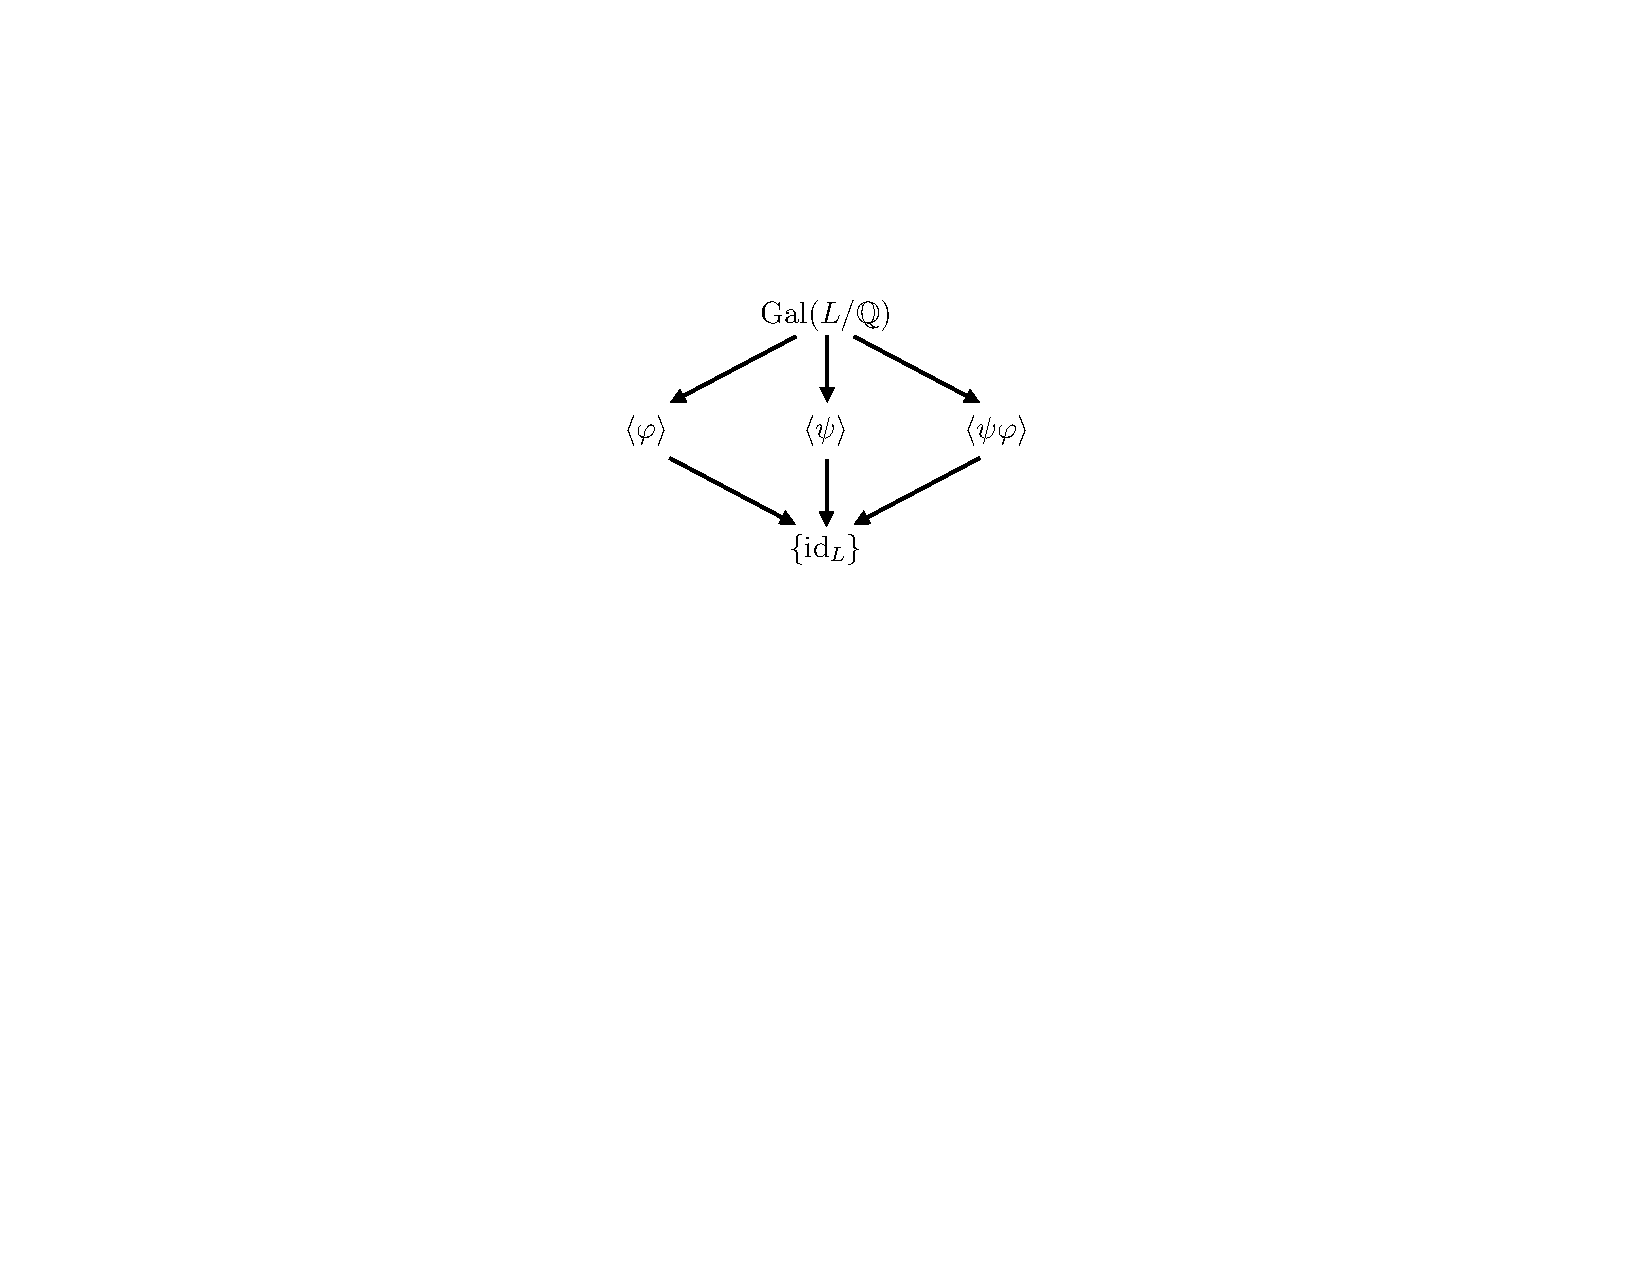
\includegraphics[width=2.3in]{pictures/galois_lattice1-1.pdf} 
\end{figure}

We have:
$$L^{\subgp{\varphi}} = \Q(\sqrt{3}), \qquad L^{\subgp{\psi}} = \Q(\sqrt{2}), \qquad
L^{\subgp{\psi\varphi}} = \Q(\sqrt{2}\sqrt{3}) = \Q({\sqrt{6}})$$
Therefore the corresponding lattice of intermediate fields of the extension $L/\Q$ looks 
as follows:
\begin{figure}[h] 
   \centering
   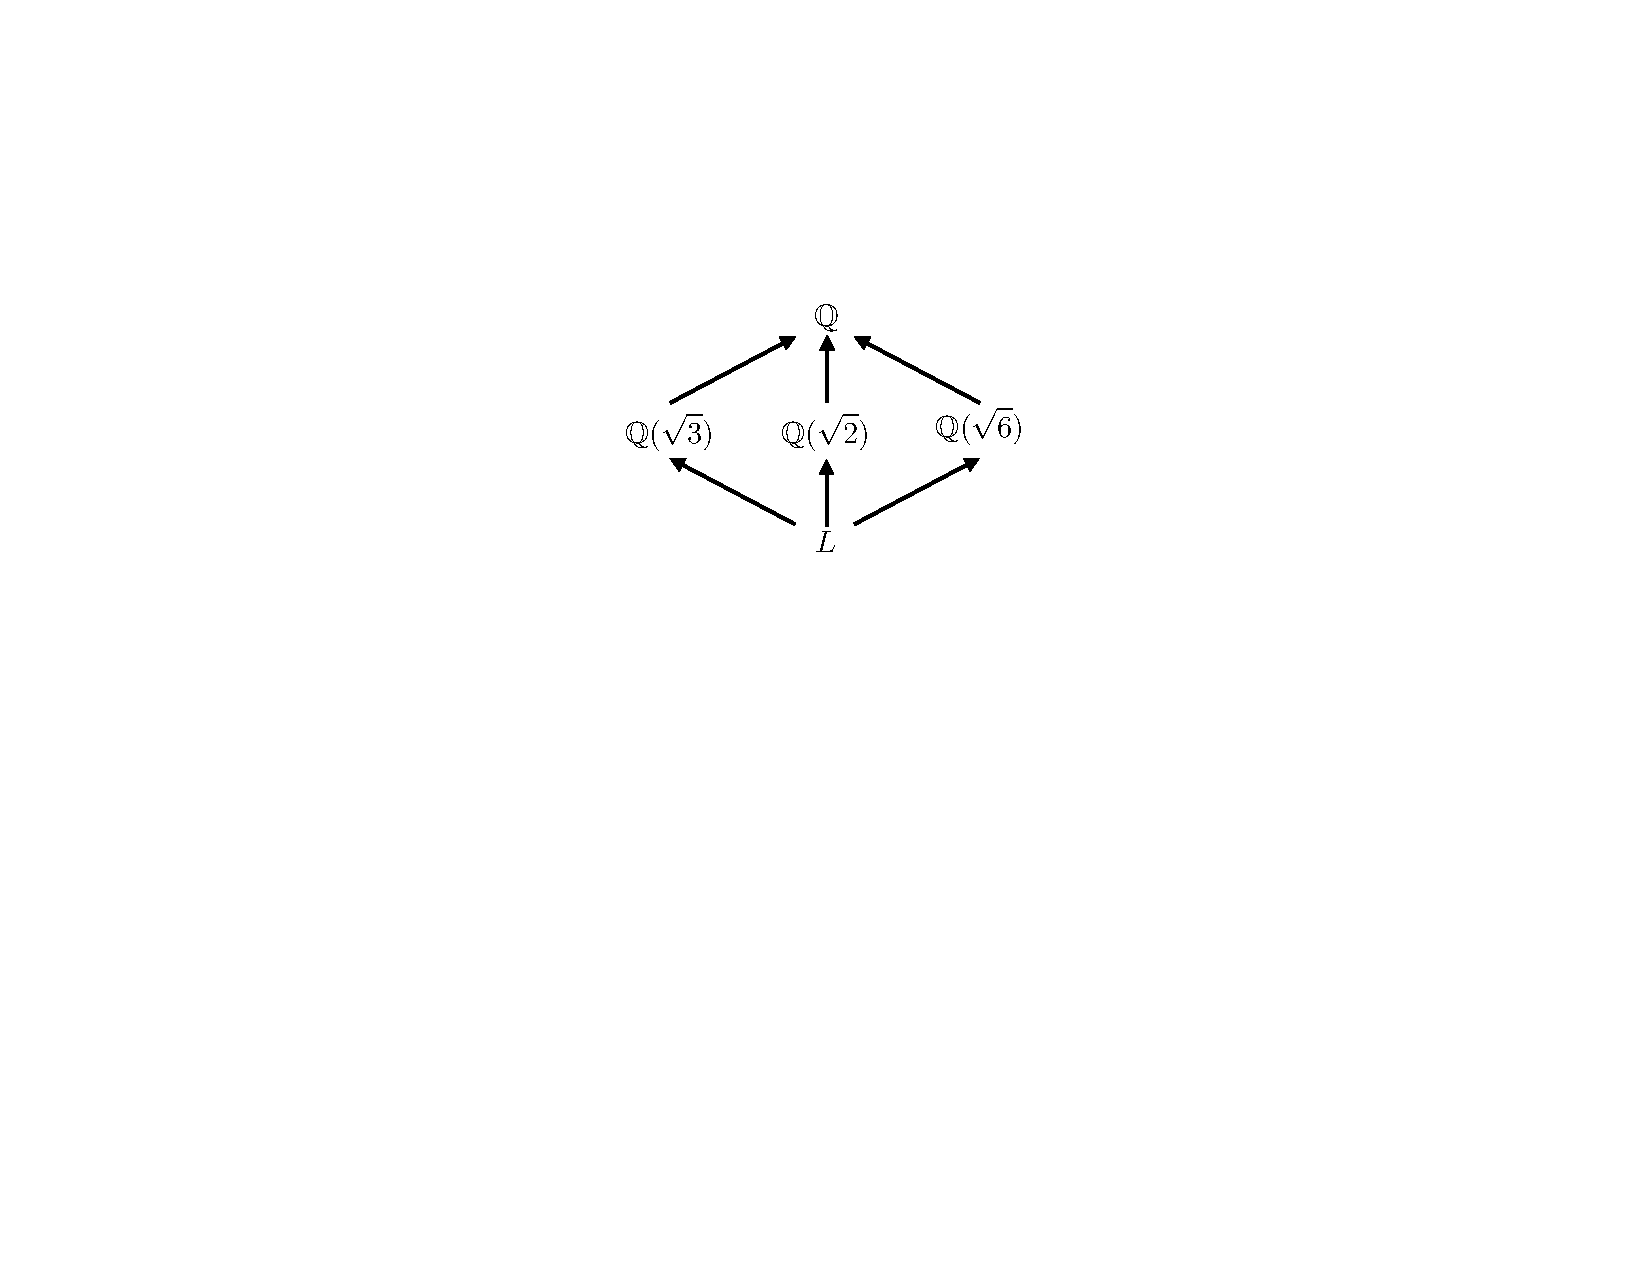
\includegraphics[width=2.3in]{pictures/galois_lattice1-2.pdf} 
\end{figure}

Notice that since $\Gal(L/\Q)$ is abelian all of its subgroups are normal and so 
all extensions $M/\Q$ where $M= \Q(\sqrt{2}), \ \Q(\sqrt{3}), \ \Q(\sqrt{6})$ are Galois extensions. 


\end{example}


\vs\vs

\begin{example} \ 

Take the polynomial $p(x) = x^{4} -2 \in \Q[x]$, and let $L\subseteq \C$ be a splitting field of $f(x)$. 
The roots of $p(x)$ in $\C$ are $\pm ^{4}\!\!\sqrt{2}$ and $\pm i ^{4}\!\!\sqrt{2}$, so we have 
$$L= \Q(^{4}\!\!\sqrt{2}, i)$$
Since $p(x)$ is irreducible in $\Q[x]$ we have $[\Q(^{4}\!\!\sqrt{2}):\Q] =4$. Also, 
$[L : \Q(^{4}\!\!\sqrt{2})] =2$, so we obtain 
$$[L:\Q] = [L : \Q(^{4}\!\!\sqrt{2})] \cdot [\Q(^{4}\!\!\sqrt{2}):\Q] = 8$$
Thus $|\Gal(L/\Q)| = 8$. 

If $\sigma\in \Gal(L/\Q)$ then $\sigma$ is determined by the values of $\sigma( ^{4}\!\!\sqrt{2})$
and $\sigma(i)$. The possible values of $\sigma( ^{4}\!\!\sqrt{2})$ are $\pm  ^{4}\!\!\sqrt{2}$
and $\pm i  ^{4}\!\!\sqrt{2}$, while the possible values of $\sigma(i)$ are $\pm i$. 
This gives 8 possible combinations, and since $\Gal(L/\Q)$ has 8 elements each of these 
combinations defines an element of $\Gal(L/\Q)$. 

Let $\varphi, \psi\in \Gal(L/\Q)$ be the automorphism given by 

\vskip -10mm


\ 
\begin{align*}
\varphi( ^{4}\!\! \sqrt{2}) = i {}^{4}\!\!\sqrt{2}, &\qquad  \varphi(i) = i  \\
\psi( ^{4}\!\!\sqrt{2}) =  {}^{4}\!\!\sqrt{2},   & \qquad  \psi(i) = -i \\
\end{align*}

\vskip -10mm


Notice that 
$$\psi\varphi({}^{4}\!\!\sqrt{2}) = -i {}^{4}\!\!\sqrt{2}\neq i {}^{4}\!\!\sqrt{2} = \varphi\psi({}^{4}\!\!\sqrt{2})$$
so $\Gal(L/\Q)$ is a non-abelian group. We have a group homomorphism 
$$f\colon \Gal(L/\Q) \to \Z/2$$
where for $\sigma \in \Gal(L/\Q)$ we set $f(\sigma) = 0$ if $\sigma(i) = i$ and $f(\sigma) = 1$
if $\sigma(i) =-i$. Notice that $\Ker(f)$ is the subgroup generated by $\varphi$, and since 
$|\varphi| =4$ we have  $\Ker(f)\cong \Z/4\Z$. 
We also have a group homomorphism 
$$g\colon \Z/2\Z\to \Gal(L/\Q)$$ 
such that $g(1) =\psi$. Since $fg = \id_{\Z/2\Z}$ by Proposition \ref{PROP_SEMIDIRSPLIT} we obtain 
that $\Gal(L/\Q)$ is isomorphic to the semidirect product:  
$$\Gal(L/\Q) \cong \Z/4\Z \rtimes \Z/2\Z \cong \subgp{\varphi}\rtimes \subgp{\psi}$$
which means that $\Gal(L/\Q)$ is isomorphic to the dihedral group $D_{4}$ (\ref{EX_SEMIDIRPROD}).
In particular every element of $\Gal(L/\Q)$ is of the form $\varphi^{i}\psi^{j}$ for $0\leq i \leq 3$, 
$0\leq j \leq 1$. 

The lattice of subgroups of $\Gal(L/\Q)$ looks as follows:

\ 


\begin{figure}[h] 
   \centering
   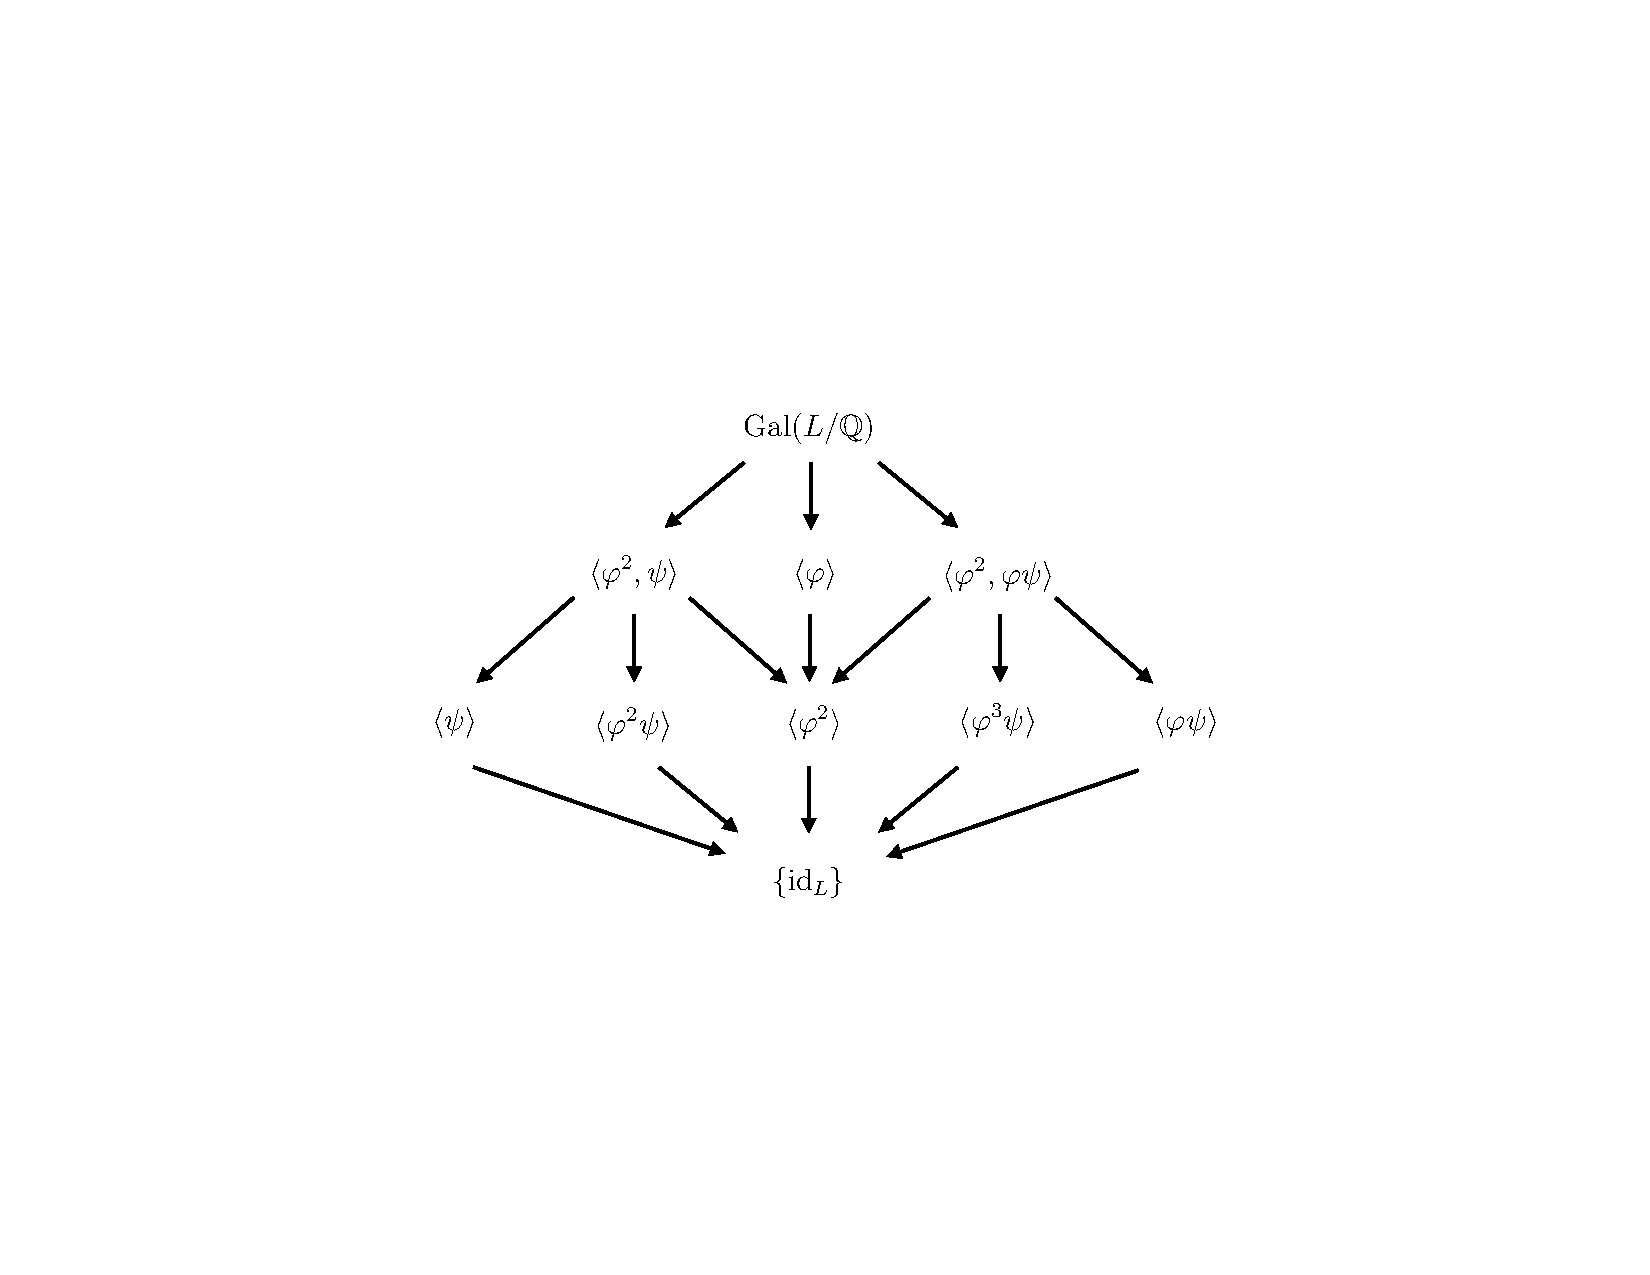
\includegraphics[width=4.2in]{pictures/galois_lattice2-1.pdf} 
  \end{figure}


This corresponds to the following lattice of intermediate fields of $L/\Q$:

\begin{figure}[h] 
   \centering
   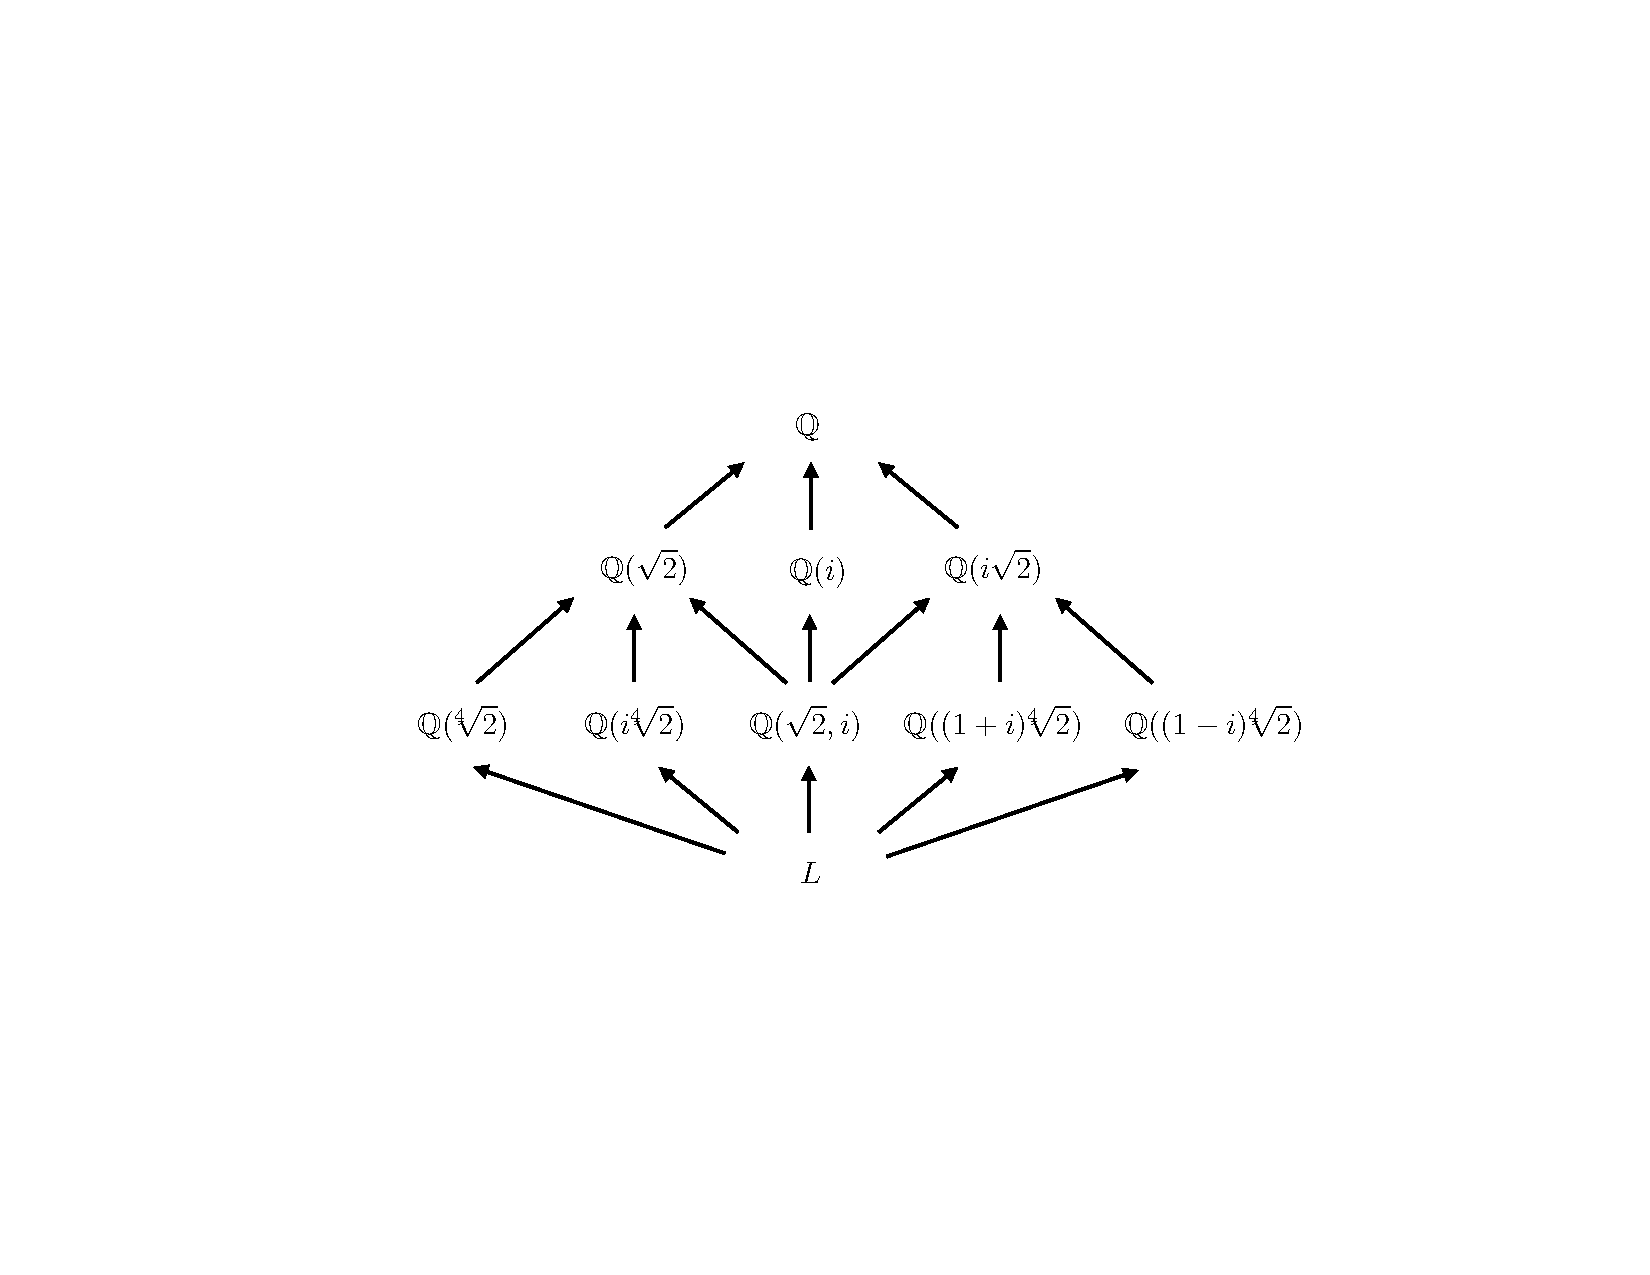
\includegraphics[width=5in]{pictures/galois_lattice2-2.pdf} 
\end{figure}
 

\end{example}




%%%%%%%%%%%%%%%%%%%%%%%%%%%%%%%
%%%%%%%%%%%%%%%%%%%%%%%%%%%%%%%
%%%
%%%  THE FUNDAMENTAL THEOREM OF ALGEBRA
%%%
%%%%%%%%%%%%%%%%%%%%%%%%%%%%%%%
%%%%%%%%%%%%%%%%%%%%%%%%%%%%%%%





\newpage
\section{The fundamental theorem of algebra}
\label{SEC_FUNDTHMALGEBRA}

Recall:

\textbf{\ref{THM_FTALG} Fundamental Theorem of Algebra.}
\emph{The field $\C$ of complex numbers is algebraically closed.}


\vs\vs

\begin{lemma} \ 
\label{LEMMA_CRPOLYROOTS}
1) If $f(x)\in \R[x]$ is a polynomial of an odd degree then $f(x)$ has a root in $\R$. 
In particular  if $f(x)\in \R[x]$ is a polynomial of an odd degree then $f(x)$ is irreducible 
iff  $\deg f(x) =1$.

2) If $f(x)\in \C[x]$ is a polynomial of degree 2 then $f(x)$ splits over  $\C$. In particular 
there are no extensions $L/\C$ such that $[L:\C]=2$.

\end{lemma}

\vs

\begin{proof}
Exercise. 
\end{proof}


\vs\vs

\begin{lemma}
\label{LEMMA_ODDEXTOFR}
If $L/\R$ is an algebraic extension, $[L:\R]<\infty$, and $[L:\R]$ is an odd number then $L=\R$. 
\end{lemma}

\vs

\begin{proof}
Since $L/\R$ is a separable extension and $[L:\R]< \infty$ thus by (\ref{THM_SEPEXTISSIMPLE})
we have $L = \R(a)$ for some $a\in L$. Let $f(x) = \irr^{\R}_{a}(x)$. 
Then $\deg f(x) = [L:\R]$ is an odd number. Since $f(x)$ is an irreducible polynomial by 
Lemma \ref{LEMMA_CRPOLYROOTS} we obtain $[L:\R] = \deg f(x)  =1$. Thus
$L = \R$. 
\end{proof}


\vs\vs

\begin{lemma}
\label{LEMMA_RALGEXTS}
If $L/\R$ is an algebraic extension such that  $[L:\R] < \infty$ then $[L:\R] = 2^{n}$ 
for some $n\geq 0$. 
\end{lemma}


\vs

\begin{proof}
Assume that there exists an odd prime  $p$ such that $p\mid [L:\R]$. Let $M$ be a normal closure 
of the extension $L/K$. We have 
$$[M:\R] = [M:L]\cdot [L:\R]$$
so $p\mid [M: \R]$. 

Let $P$ be the Sylow $2$-subgroup of $\Gal(M/\R)$. Since $M/\R$ is a Galois extension we have 
$|\Gal(M/\R)| = [M:\R]$, and so $p\mid |\Gal(M/\R)|$. On the other hand  
$p\nmid |P|$ so  $P\neq \Gal(M/\R)$. It follows that $M^{P} \neq M^{\Gal(M/\R)} = \R$. 
Moreover we have 
$$[M:\R] = [M:M^{P}]\cdot [M^{P}: \R] $$
so: 
$$[M^{P}:\R] = [M:\R]/[M:M^{P}] = |\Gal(M/\R)|/|P|$$
and so $[M^{P}:\R]$ is an odd number. 

As a consequence we obtain that $M^{P}/\R$ is an extension of an odd degree and that 
$M^{P}\neq \R$. This is however impossible by Lemma \ref{LEMMA_ODDEXTOFR}. 



\end{proof}

\vs\vs


\begin{proof}[Proof of Theorem \ref{THM_FTALG}]  \ 

Let $L/\C$ be an algebraic extension, $[L:\C]< \infty$,  and let 
$M$ be a normal closure of $L/\C$. Then $M/\C$ is a Galois extension. 
We have 
$$[M:\R] = [M:\C]\cdot [\C: \R] = 2[M:\C]$$
By Lemma \ref{LEMMA_RALGEXTS}  we have $[M:\R] = 2^{n}$ for some $n$,  and thus 
$[M:\C] = 2^{n-1}$. 

Assume that $n-1>0$. Then  $\Gal(M/\C)$ is a non-trivial 2-group, and so it has 
a normal subgroup $H$ such that 
$$\Gal(M/\C)/H \cong \Z/2\Z$$
By Theorem \ref{THM_FUNDGALOISTHM} we obtain that $M^{H}/\C$ is 
a Galois extension and
$$[M^{H}:\C] = |\Gal(M^{H}/\C)| = |\Z/2\Z|=2$$
which is impossible by Lemma \ref{LEMMA_CRPOLYROOTS}. 

Therefore  $[M:\C] = 1$, i.e. $M = \C$. Since $\C \subseteq L \subseteq M$
this also gives that $L = \C$.  As a consequence  we obtain that there are 
no non-trivial algebraic extensions of $\C$.  By Proposition \ref{PROP_ALGCLOSEDPROPS}
this shows that $\C$ is an algebraically closed field. 
\end{proof}








%%%%%%%%%%%%%%%%%%%%%%%%%%%%%%%
%%%%%%%%%%%%%%%%%%%%%%%%%%%%%%%
%%%
%%%  INFINITE GALOIS EXTENSIONS
%%%
%%%%%%%%%%%%%%%%%%%%%%%%%%%%%%%
%%%%%%%%%%%%%%%%%%%%%%%%%%%%%%%




\newpage
\section{Infinite Galois extensions}
\label{SEC_INFINITEGALEXT}


\begin{note}
If $L/K$ is a Galois extension such that $[L:K]=\infty$ then the maps 
$$
\Phi\colon 
\begin{pmatrix}
\text{ intermediate fields} \\[1mm]
\text{  $K\subseteq M \subseteq L$} \\
\end{pmatrix}
\ \leftrightarrows \ 
\begin{pmatrix}
\text{subgroups} \\[1mm]
\text{ $H\subseteq \Gal(L/K)$} \\
\end{pmatrix}
\colon \Psi
$$
need not be bijections since not every subgroup of of $\Gal(L/K)$ will be of the form 
$\Gal(L/M)$ for some intermediate field $M$.  
\end{note}

\vs\vs

\begin{example} \ 

Take 
$$L = \Q(\sqrt{2}, \sqrt{3}, \sqrt{5}, \dots )$$
Then $L/\Q$ is a Galois extension, $[L:\Q] = \infty$. 

If $\sigma\in \Gal(L/\Q)$ then $\sigma(\sqrt{p}) = \pm \sqrt{p}$ for each prime $p$. This gives 
$\sigma^{2} = \id_{L}$, so all elements of $\Gal(L/\Q)$ are of order $2$, and so $\Gal(L/\Q)$
is an infinite dimensions vector space over $\F_{2}$. If follows that $\Gal(L/\Q)$ has uncountably
many subgroups $H$ such that $[\Gal(L/\Q) : H] = 2$ (check).  

Let  $H$ be such subgroup and assume that we have an intermediate field 
$K\subseteq M \subseteq L$ such that $\Gal(L/M) =H$. Since $H$ is a normal subgroup of 
$\Gal(L/\Q)$ we obtain that $M/\Q$ is a Galois extension and 
$$\Gal(M/\Q) = \Gal(L/\Q)/H \cong \Z/2\Z$$
In particular $[M/\Q] = 2 <\infty $, so by  (\ref{THM_SEPEXTISSIMPLE}) we have 
$M = K(a)$ for some $a \in \R$, $\deg_{\Q}(a) =2$. The set of such elements $a$
is countable, so  there are only countably many such intermediate fields $M$. As a consequence 
there is a subgroup  $H\subseteq \Gal(L/\Q)$ such that $H\neq \Gal(L/M)$ for any intermediate 
field $M$.


\end{example}

\vs

In order to fix it we need to describe, given a Galois extension $L/K$,  which subgroups of 
$\Gal(L/K)$ are of the form $\Gal(L/M)$ for some intermediate field $K\subseteq M\subseteq L$. 

\vs\vs


Let $L/K$ be an algebraic field extension and let $A=\{ a_{1}, \dots, a_{n}\}$, $B=\{b_{1}, \dots, b_{n}\}$ be 
finite subsets of $L$. Denote
$$U(A, B) := \{\sigma\in \Gal(L/K) \ | \ \sigma(a_{i}) = b_{i} \}$$ 

\vs

\begin{definition/proposition}
For any algebraic field extension $L/K$ the collection of subsets 
$$\mathcal{U} := \{ U(A, B) \subseteq \Gal(L/K) \ | \ A, B \subseteq L, \ |A| = |B| < \infty \}$$
is a basis of some topology on $\Gal(L/K)$. This topology is called the \emph{Krull topology}. 
\end{definition/proposition}

\vs\vs

\begin{proposition}
Let $L/K$ be a algebraic field extension. If $K\subseteq M\subseteq L$ is an intermediate field. 
then $\Gal(L/M)$ is a closed subset of $\Gal(L/K)$.
\end{proposition}

\vs

\begin{proof}
Let $\overline{\Gal(L/M)}$ denote the closure of $\Gal(L/M)$ in the Krull topology on $\Gal(L/K)$. 
We will show that $\overline{\Gal(L/M)} = \Gal(L/M)$. 

Let $\psi\in \overline{\Gal(L/M)}$. Take an element $a\in M$ and let 
$$A:=\{a\}, \ \ \  B:= \{\psi(a) \}$$
Then $U(A, B)$ is an open neighborhood of $\psi$ in $\Gal(L/K)$. Since 
$\psi\in  \overline{\Gal(L/M)}$ there exists $\varphi\in U(A, B)$ such that $\varphi\in \Gal(L/M)$.
We have 
$$\varphi(a) = \psi(a)$$
On the other hand, since $a\in M$ we have $\varphi(a) = a$. Therefore we obtain 
$\psi(a) = a$.  Since this holds for an arbitrary element $a\in M$ we get that $\psi\in \Gal(L/M)$. 

\end{proof}


\vs\vs\vs\vs

\begin{proposition}
Let $L/K$ be a Galois extension and let $H\subset \Gal(L/K)$ be a closed subgroup. Then 
$H = \Gal(L/L^{H})$.
\end{proposition}


\vs

\begin{proof}
We have $H\subseteq \Gal(L/L^{H})$. Conversely, let $\varphi\in \Gal(L/L^{H})$. We will show 
that $\varphi\in H$. 

We argue by contradiction. Assume that $\varphi\not\in H$. Since $H$ is a closed subgroup
there exists an open neighborhood $U(A, B)\subseteq \Gal(L/K)$ such that $\varphi\in U(A, B)$
and $H \cap \Gal(L/L^{H}) = \varnothing$.  

Let $A= \{ a_{1}, \dots, a_{n}\}$ and let $N\subseteq L$
be the normal closure of $L^{H}(a_{1}, \dots, a_{n})$. Since $N/L^{H}$ is a normal extension 
for any $\psi \in \Gal(L/L^{H})$ we have $\psi(N) = N$. Define 
$$H' := \{ \psi|_{N}\colon N\to N \ | \ \psi\in H \} \subseteq \Gal(N/L^{H})$$
Notice that $\varphi|_{N}\not\in H'$, so $H'\neq \Gal(N/L^{H})$. 
Since $N/L^{H}$ is a Galois extension and $[N:L^{H}] <\infty$ by the Fundamental Theorem of 
Galois Theory (\ref{THM_FUNDGALOISTHM})  we obtain 
$$N^{H'} \neq N^{\Gal(N/L^{H})} = L^{H}$$
On the other hand if $a\in N^{H'}$ then $\psi(a) = a$ for all $\psi\in H$, so $a\in L^{H}$. Thus 
$N^{H'} \subseteq L^{H}$. Since obviously we also have $L^{H}\subseteq N^{H'}$ we get 
$N^{H'} = L^{H}$ which is a contradiction. 

\end{proof}


\vs\vs

\begin{corollary}
If $L/K$ is a Galois extension then the maps 
$$
\Phi\colon 
\begin{pmatrix}
\text{ intermediate fields} \\[1mm]
\text{  $K\subseteq M \subseteq L$} \\
\end{pmatrix}
\ \leftrightarrows \ 
\begin{pmatrix}
\text{closed subgroups} \\[1mm]
\text{ $H\subseteq \Gal(L/K)$} \\
\end{pmatrix}
\colon \Psi
$$
given by $\Phi(M) = \Gal(L/M)$,  $\Psi(H) = L^{H}$
are bijections and $\Psi = \Phi^{-1}$. 
\end{corollary}


\vs\vs

\begin{note}
If $L/K$ is a Galois extension such that $[L:K]<\infty$ then  Krull topology on $\Gal(L/K)$
is the discrete topology (check!), and so any subgroup of $\Gal(L/K)$ is a closed subgroup. 
\end{note}





%%%%%%%%%%%%%%%%%%%%%%%%%%%%%%%
%%%%%%%%%%%%%%%%%%%%%%%%%%%%%%%
%%%
%%%  ABELIAN AND CYCLIC EXTENSIONS
%%%
%%%%%%%%%%%%%%%%%%%%%%%%%%%%%%%
%%%%%%%%%%%%%%%%%%%%%%%%%%%%%%%


\newpage
\section{Abelian and cyclic extensions}
\label{SEC_ABANDCYCEXT}

\begin{definition}
Let $L/K$ be a Galois extension, $[L:K] < \infty$. The extension $L/K$ is 
\emph{abelian} (resp. \emph{cyclic}) if the group $\Gal(L/K)$ is abelian 
(resp. cyclic). 
\end{definition}

\vs\vs


\begin{proposition}
If $L/K$ is an abelian (resp. cyclic) extension and $M$ is an intermediate field 
then $L/M$ and $M/K$ are also abelian (resp. cyclic) extensions. 
\end{proposition}


\vs

\begin{proof}
Exercise. 
\end{proof}


\vs\vs

\begin{definition}
\label{DEF_CYCLOTEXT}
An extension $L/K$ is a \emph{cyclotomic extension of degree $n$}  if $L$ is a splitting 
field of the polynomial $f(x) = x^{n} -1 \in K[x]$. 
\end{definition}


\vs\vs


\begin{note}
If $\chi(K)=p\neq 0$ and $n=mp^{k}$ then $x^{n}-1 = (x^{m} -1)^{p^{k}}$, so 
cyclotomic extensions of orders $n$ and $m$ coincide. Thus we can always assume 
that $p\nmid n$. 
\end{note}


\vs\vs



\begin{theorem}
\label{THM_CYCLOTEXT}
Let $L/K$ be a cyclotomic extension of degree $n$. If $\chi(K) = p\neq 0$ assume that 
$p\nmid n$. Then 

\vskip -13mm

\benu
\item $L = K(\zeta)$ where $\zeta$ is a primitive $n$-th root of unity;
\item $\Gal(L/K)$ is isomorphic to a subgroup of $(\Z/n\Z)^{\ast}$, the multiplicative 
of units of the ring $\Z/n\Z$.
\eenu

\end{theorem}

\vs\vs\vs\vs

\begin{proof} \ 

1) \ Since   $L$ is a splitting field of $f(x) = x^{n}-1$ thus $L$ contains a primitive  $n$-th 
root of unity. Moreover, every other root  of $f(x)=x^{n}-1$ in $L$ is of the form $\zeta^{k}$
for some $1\leq k \leq n$, so $L = K(\zeta)$. 

\vs 

2) If $\varphi\in \Gal(L/K)$ then $\varphi$ is uniquely determined determined by the
value of $\varphi(\zeta)\in L$. Since $\zeta$ is a primitive $n$-th root of unity 
$\varphi(\zeta)$ also must be a primitive $n$-th root of unity. This means that 
$\varphi(\zeta) = \zeta^{k}$ where $1\leq k \leq n$,  $\gcd(n, k)=1$. 

Define a map 
$$\Phi\colon \Gal(L/K) \to (\Z/n\Z)^{\ast}$$
where $\Phi(\varphi) = k$ if $\varphi(\zeta) = \zeta^{k}$.  
Then  $\Phi$ is a monomorphism and it is a homomorphism of groups (check!). 
It follows that $\Gal(L/K)$ is isomorphic to the subgroup $\Phi(\Gal(L/K))\subseteq (\Z/n\Z)^{\ast}$.

\end{proof}

\vs\vs

\begin{note}
\label{NOTE_CYCLOTEXTQ}
If $L$ is the cyclotomic extension of $\Q$ of degree $n$ then 
$$\Gal(L/\Q) \cong (\Z/n\Z)^{\ast}$$
(see Hungerford Ch. V, Proposition 8.3). 
\end{note}

\vs\vs

\begin{corollary}
If $L/K$ is a cyclotomic extension of degree $n$ then $L/K$ is an abelian extension. 
Moreover, if $n$ is  a prime number and $\chi(K)\nmid n$ then $L/K$ is a cyclic extension. 
\end{corollary}

\vs

\begin{proof}
By Theorem \ref{THM_CYCLOTEXT} the group $\Gal(L/K)$ can be identified with a subgroup of 
$(\Z/n\Z)^{\ast}$. Since the group  $(\Z/n\Z)^{\ast}$ is abelian thus so is $\Gal(L/K)$. 

If $n$ is prime then $(\Z/n\Z)^{\ast}$ is a cyclic group 
(see Proposition \ref{PROP_FINMULTSUBGPDOMAIN}), so $\Gal(L/K)$ is cyclic.
\end{proof}


\vs\vs

\begin{theorem}[Kronecker-Weber]\  \\
If $L/\Q$ is an abelian extension then $L\subseteq M$ where $M/\Q$ is some cyclotomic 
extension of $\Q$. 
\end{theorem}


\vs

\begin{proof}
See e.g.: 

\href{http://www.jstor.org/stable/2319208}
{
M.J. Greenberg, \emph{An elementary proof of the Kronecker-Weber theorem}, 
The American Mathematical Monthly 81(6) (1974), 601-607.
 }

 (with erratum in 
 \href{http://www.jstor.org/stable/2319794}{
  The American Mathematical Monthly 82(8) (1975), 803})
 
\end{proof}

\vs\vs


\begin{theorem}
\label{THM_LAGRANGECYCEXT}
Let $K$ be a field such that $K$ contains a primitive $n$-th root of unity $\zeta$
and let  $L/K$ be a field extension. 

1) If $L/K$ is a cyclic extension and $[L:K]=n$ then $L= K(b)$ for some $b\in L$ such 
that $b^{n}\in K$

2) If $L=K(b)$ for some $b\in L$ such that $b^{n}\in K$ then $L/K$ is a cyclic extension. 


\end{theorem}


\vs\vs

\begin{lemma}
\label{LEMMA_FIELDAUTOLININDEP}
Let $L$ be a field and let $\varphi_{1}, \dots, \varphi_{n}$ be distinct automorphisms of
$L$.  For $c_{1}, \dots, c_{n}\in L$ consider the map 
$$\psi \colon L \to L, \ \ \ \ \psi(a) = \sum_{i=1}^{n} c_{i}\varphi_{i}(a)$$
If $\varphi(a)=0$ for all $a\in L$ then $c_{1}=\dots = c_{n}=0$ 
\end{lemma}

\vs 

\begin{proof}
We argue by induction with respect to $n$. 

If $n=1$ the statement is obvious. 

Assume that the statement of the lemma holds for some $n$, and  
let $\varphi_{1}, \dots, \varphi_{n+1}\in \Aut(L)$, $c_{1}, \dots, c_{n+1}\in L$
be such that 
$$\sum_{i=1}^{n+1}c_{i}\varphi_{i}(a) = 0$$
for all $a\in L$. For any $a, b\in L$, $a\neq 0$ we have 
\begin{align*}
0  &  = \sum_{i=1}^{n+1}c_{i}\varphi_{i}(ab) \\
& =  \sum_{i=1}^{n+1}c_{i}\varphi_{i}(a)\varphi_{i}(b) 
\end{align*}
Since $a\neq 0$ we have $\varphi_{n+1}(a) \neq 0$ so we have 
\begin{align*}
0 & =  \frac{1}{\varphi_{n+1}(a)}\sum_{i=1}^{n+1}c_{i}\varphi_{i}(a)\varphi_{i}(b) \\
& = \sum_{i=1}^{n+1}c_{i}\frac{\varphi_{i}(a)}{\varphi_{n+1}(a)}\varphi_{i}(b)
\end{align*}
Since also $\sum_{i} c_{i}\varphi_{i}(b)=0$ we obtain
\begin{align*}
0 & = \sum_{i=1}^{n+1}c_{i}\frac{\varphi_{i}(a)}{\varphi_{n+1}(a)}\varphi_{i}(b) - \sum_{i} c_{i}\varphi_{i}(b) \\
& = \sum_{i=1}^{n+1}c_{i}\left(\frac{\varphi_{i}(a)}{\varphi_{n+1}(a)}-1\right)\varphi_{i}(b) \\
& =  \sum_{i=1}^{n}c_{i}\left(\frac{\varphi_{i}(a)}{\varphi_{n+1}(a)}-1\right)\varphi_{i}(b)
\end{align*}
By the inductive assumption this gives 
$$c_{i}\left(\frac{\varphi_{i}(a)}{\varphi_{n+1}(a)}-1\right)=0$$
for all $i=1, \dots, n$ and all $0\neq a\in L$. If $c_{i}\neq 0$ for some $1\leq i\leq n$ this would give 
$$\varphi_{i}(a)= \varphi_{n+1}(a)$$
for all $a\in L$ which is impossible since $\varphi_{1}, \dots, \varphi_{n+1}$ are distinct automorphisms. 
Thus we obtain $c_{1}= {\dots} = c_{n} =0$, and so also $c_{n+1} = 0$.  
\end{proof}


\vs\vs

\begin{proof}[Proof of Theorem \ref{THM_LAGRANGECYCEXT}] \ 

1) \  Assume that $L/K$ is a cyclic extension, $[L:K]=n$, and let 
$\varphi$ be a generator of $\Gal(L/K)$. Let $\psi\colon L \to L$ 
be the map given by 
$$\psi(a) = \sum_{i=1}^{n} \zeta^{i}\varphi^{i}(a)$$
By Lemma \ref{LEMMA_FIELDAUTOLININDEP} there exists $a\in L$ such that 
$\psi(a)\neq 0$. 

Notice that we have 
\begin{align*}
\varphi(\psi(a)) & =  \sum_{i=1}^{n}\zeta^{i}\varphi^{i+1}(a) \\
& = \zeta^{-1} \sum_{i=1}^{n}\zeta^{i+1}\varphi^{i+1}(a) \\
& = \zeta^{-1}\psi(a)
\end{align*}

By induction we obtain
\begin{align*}
\varphi^{k}(\psi(a)) = \zeta^{-k}\psi(a)
\end{align*}
for all $k$. 
\vs

\emph{Claim 1.} $L= K(\psi(a))$.

Indeed, it is enough to show that $\deg_{K}(\psi(a)) = [L:K] = n$. 

Let $f(x) = \irr^{K}_{\psi(a)}(x)$. By (\ref{PROP_AUTOOFROOTS}) 
for any  $1\leq k \leq n$ the element  $\varphi^{k}(\psi(a))$ is a root of $f(x)$. 
Moreover,  if  $1\leq k, l \leq n$ and $k\neq l$ then we have 
$$\varphi^{k}(\psi(a)) = \zeta^{-k}\psi(a) \neq \zeta^{-l}\psi(a) = \varphi^{l}(\psi(a))$$
so $f(x)$ has $n$ distinct roots in $L$. 
It follows that $\deg f(x) \geq n$, and so $\deg_{K}(\psi(a))\geq n$. Also, since
$\psi(a)\in L$ we have $\deg_{K}(\psi(a)) \leq [L:K] = n$. Therefore $\deg_{K}(\psi(a))=n$.

\vs

\emph{Claim 2.}   $\psi(a)^{n} \in K$.

Indeed, notice that since $L/K$ is a Galois extension we have $K = L^{\Gal(L/K)}$. 
Also, since $\varphi$ generates $\Gal(L/K)$ we have 
$$K = L^{\Gal(L/K)} = \{c\in L \ | \ \varphi(c) = c \}$$
Thus it suffices to show that $\varphi(\psi(a)^{n}) = \psi(a)^{n}$. 
We have
$$\varphi(\psi(a)^{n}) = \varphi(\psi(a))^{n} = (\zeta^{-1}\psi(a))^{n} = \zeta^{-n}\psi(a)^{n} = \psi(a)$$

From Claims 1 and 2 it follows that in the statement of the theorem we can take $b= \psi(a)$. 


\vs\vs

2)  Assume that $L = K(b)$ for some $b\in L$ such that $b^{n} \in K$. 
We need to show that $L/K$ is a Galois extension and that $\Gal(L/K)$ is a cyclic group. 

Consider the polynomial $f(x) = x^{n}-b^{n}\in K[x]$. Notice that $f(x)$ has $n$ distinct roots 
$b, \zeta b, \dots, \zeta^{n-1}b\in L$.  It follows that $L$ is a splitting field of $f(x)$ and that 
$f(x)$ is a separable polynomial. As a consequence $L/K$ is a Galois extension. 

Next, notice that any automorphism $\varphi\in \Gal(L/K)$ is uniquely determined by the 
value of $\varphi(b)$, and that $\varphi(b) = \zeta^{k} b$ for some $0\leq k \leq n-1$. 

Let $\mu_{n}(K)$ denote the multiplicative group of $n$-th roots of unity in $K$ 
(\ref{PROP_GPOFROOTSOFUNITY}). Define a map 
$$\Phi \colon \Gal(L/K) \to  \mu_{n}(K)$$
by $\Phi(\varphi) = \zeta^{k}$ if $\varphi(b) = \zeta^{k}b$. Then $\Phi$ is a monomorphism, 
and it is a homomorphism of groups (check!). It follows that $\Gal(L/K)$ is isomorphic
to a subgroup of $\mu_{n}(K)$. By (\ref{THM_ROOTSOFUNITYCYCLIC}) the group 
$\mu_{n}(K)$ is cyclic, and so $\Gal(L/K)$ is also a cyclic group. 

 


\end{proof}





%%%%%%%%%%%%%%%%%%%%%%%%%%%%%%%
%%%%%%%%%%%%%%%%%%%%%%%%%%%%%%%
%%%
%%%  RADICAL EXTENSIONS
%%%
%%%%%%%%%%%%%%%%%%%%%%%%%%%%%%%
%%%%%%%%%%%%%%%%%%%%%%%%%%%%%%%


\newpage
\section{Radical extensions}
\label{SEC_RADICALEXT}





\begin{definition}
A field extension $L/K$ is a \emph{radical extension}  if there exist elements 
$a_{1}, \dots, a_{n}\in L$ such that $L = K(a_{1}, \dots, a_{n})$ and for every $i=1, \dots, n$
there exists $m_{i}\geq 1$ such that 
$$a_{i}^{m_{i}}\in K(a_{1}, \dots, a_{i-1})$$  
\end{definition}

\vs\vs


\begin{definition}
Let $\bar{K}$ be an algebraic closure of a field $K$. An element $a\in \bar{K}$ 
\emph{can be expressed by radicals} over $K$ if $a\in L$ for some radical extension 
$L/K$. 
\end{definition}

\vs\vs


\begin{note}
An element $a\in \bar{K}$ can expressed by radicals over $K$ iff $a$ can be obtained 
from elements of $K$ using arithmetic operators $+$, $-$, $\cdot$, $/$ and root extraction.  
\end{note}


\vs\vs



\begin{definition}
A polynomial $f(x)\in K[x]$ \emph{can be solved by radicals}  if all roots of $f(x)$
can be expressed by radicals over $K$. 
\end{definition}


\vs\vs



\begin{proposition}
\label{PROP_RADICALSPLITFIELD}
If $f(x)\in K[x]$ and $L$ is a splitting field of $f(x)$ then $f(x)$ can be solved by radicals 
iff $L\subseteq M$ where $M/K$ is a radical extension. 
\end{proposition}



\vs\vs


\begin{lemma}
\label{LEMMA_MNRADEXT}
If $\bar{K}$ is an algebraic closure of $K$ and $L/K$, $M/K$ are radical extensions 
such that $L, M\subseteq \bar{K}$ then $LM/K$ is also a radical extension.  
\end{lemma}


\vs

\begin{proof}
Exercise. 
\end{proof}


\vs\vs

\begin{proof}[Proof of Proposition \ref{PROP_RADICALSPLITFIELD}] \ 

($\Rightarrow$) \ Let $L= K(a_{1}, \dots, a_{n})$ where $a_{1}, \dots, a_{n}$ are roots of $f(x)$. 
Let $\bar{K}$ be an algebraic closure of $K$ such that $L\subseteq \bar{K}$. 
By assumption for every $a_{i}$ there exists $L_{i}\subseteq \bar{K}$ such that $a_{i}\in L_{i}$
and $L_{i}/K$ is a radical extension. Then we have 
$$L = K(a_{1}, \dots, a_{n})\subseteq L_{1}L_{2}\cdots L_{n}$$
and by Lemma \ref{LEMMA_MNRADEXT}  $L_{1}L_{2}\cdots L_{n}/K$ is a radical extension. 

\vs 

($\Leftarrow$) \ Obvious. 

\end{proof}


\vs\vs

\begin{proposition}
\label{PROP_NORMCLRADEXT}
Let $L/K$ be a radical extension. If $N$ is a normal closure of $L/K$ then $N/K$
is also a radical extension. 
\end{proposition}


\vs

\begin{proof}
Let $N$ be a normal closure of of $L/K$. We have:
$$N = \prod_{\varphi\in \Gal(N/K)} \varphi(L)$$
(exercise). Since $L/K$ is a radical extension thus for every $\varphi\in \Gal(L/K)$ 
the extension $\varphi(L)/K$ is also a radical extension (check!). 
By Lemma \ref{LEMMA_MNRADEXT} it follows that 
that  $\left(\prod_{\varphi\in \Gal(N/K)} \varphi(L)\right)/K$ is also a radical extension. 
\end{proof}




%%%%%%%%%%%%%%%%%%%%%%%%%%%%%%%
%%%%%%%%%%%%%%%%%%%%%%%%%%%%%%%
%%%
%%%  SOLVABLE EXTENSIONS
%%%
%%%%%%%%%%%%%%%%%%%%%%%%%%%%%%%
%%%%%%%%%%%%%%%%%%%%%%%%%%%%%%%


\newpage
\section{Solvable extensions}
\label{SEC_SOLVEXT}




\textbf{Recall. } 

\textbf{\textbullet} \ A group $G$ is \emph{solvable} if it has a normal series
$$\{e\}= G_{0} \subseteq {\dots} \subseteq G_{k} = G$$
such that for every $i$ the group $G_{i}/G_{i-1}$ is abelian.


\textbf{\textbullet} \ Abelian groups and finite $p$-groups are solvable. 


\textbf{\textbullet} \ The symmetric group $S_{n}$ is solvable iff $n\leq 4$. 

\textbf{\textbullet} \ Subgroups and quotients groups of a solvable group are solvable. 


\textbf{\textbullet} \ If $H\lhd G$ and $H$, $G/H$ are solvable groups then  $G$ is solvable.  


\vs\vs


\begin{definition}
A Galois extension $L/K$ is \emph{solvable} if $[L:K]<\infty$ and $\Gal(L/K)$ is a 
solvable group. 
\end{definition}

\vs\vs

\begin{theorem}
\label{THM_RADICALVSSOLVABLEEXT}
Let $L/K$ be a Galois extension such that $[L:K] < \infty$ and $\chi(K) = 0$.
The following conditions are equivalent:
\vskip -13mm

\ 
\benu
\item[(i)] \ There exists a radical extension $M/K$ such that $L\subseteq M$. 
\item[(ii)] \ $L/K$ is a solvable extension. 
\eenu
\end{theorem}

\vs

\begin{note}
Theorem \ref{THM_RADICALVSSOLVABLEEXT} holds also if $\chi(K) = p \neq 0$ and 
$p\nmid [L:K]$. 
\end{note}


\vs\vs


\begin{corollary}
\label{COR_SOLGALSOLVRADPOLY}
If $K$ is a field, $\chi(K) = 0$,  $f(x)\in K[x]$  and $L$ is a splitting field of $f(x)$ then 
$f(x)$ can be solved by radicals iff $L/K$ is a solvable extension.   
\end{corollary}


\vs

\begin{proof}
Follows from Proposition \ref{PROP_RADICALSPLITFIELD} and 
Theorem \ref{THM_RADICALVSSOLVABLEEXT}. 
\end{proof}


\begin{proof}[Proof of Theorem \ref{THM_RADICALVSSOLVABLEEXT}]\ 

(i) $\Rightarrow$ (ii) \ It is enough to show that for any radical Galois extension 
$N/K$ the group $\Gal(N/K)$ is solvable. 

Indeed, if $L\subseteq M$ where $M/K$ is a radical extension then let 
$N$ be a normal closure of $M/K$. By Proposition \ref{PROP_NORMCLRADEXT}
$N/K$ is a radical Galois extension. We have 
$$K\subseteq L \subseteq N$$
Since $L/K$ is a Galois extension the group $\Gal(N/L)$ is a normal subgroup of 
$\Gal(N/K)$, and 
$$\Gal(L/K)\cong \Gal(N/K)/ \Gal(N/L)$$ 
Therefore if $\Gal(N/K)$ is solvable then so is $\Gal(L/K)$. 

\vs 

Assume then that $N/K$ is a radical Galois extension. Then we have 
 $a_{1}, \dots, a_{n}\in N$  such that
$$N= K(a_{1}, \dots, a_{n})$$
and  $a_{i}^{m_{i}}\in K(a_{1}, \dots, a_{i-1})$
for some  $m_{i}\geq 1$.  Denote $L_{i} := K(a_{1}, \dots, a_{i})$. We have 
$$K= L_{0}\subseteq L_{1} \subseteq {\dots}\subseteq L_{n} = N$$
This gives 
\begin{equation*}
\tag{$\ast$}
\Gal(N/K) = \Gal(N/L_{0}) \supseteq \Gal(N/L_{1}) \supseteq  
{\dots} \supseteq \Gal(N/L_{n}) = \{\id_{N}\} 
\end{equation*}


Let $\zeta\in \bar{K}$ be a primitive root of unity of order $m_{1}m_{2}\cdots m_{n}$. 
Assume first that $\zeta\in K$. 


\vs

\emph{Claim.} For every $i=1, \dots, n$ the group $\Gal(N/L_{i})$ is a normal subgroup of 
$\Gal(N/L_{i-1})$ and $\Gal(N/L_{i-1})/\Gal(N/L_{i})$ is a cyclic group. 

Indeed, $L_{i} = L_{i-1}(a_{i})$ and $a_{i}^{m_{i}}\in L_{i-1}$, and $L_{i-1}$ contains
a primitive root of unity of degree $m_{i}$,  so by Theorem \ref{THM_LAGRANGECYCEXT} 
$L_{i}/L_{i-1}$ is a cyclic Galois extension. We have 
$$ L_{i-1} \subseteq L_{i} \subseteq N$$
Since $L_{i}/L_{i-1}$ is a Galois extension thus $\Gal(N/L_{i})$ is a normal subgroup of 
$\Gal(N/L_{i-1})$ and 
$$\Gal(N/L_{i-1})/\Gal(N/L_{i})\cong \Gal(L_{i}/L_{i-1})$$



As a consequence we obtain that the sequence ($\ast$) is a normal series of $\Gal(N/K)$
with cyclic quotients, and so $\Gal(N/K)$ is a solvable group. 



Next, assume that  $K$ does not contain the primitive root $\zeta$. In such case consider 
the extensions
$$K\subseteq K(\zeta) \subseteq N(\zeta)$$
The extensions  $N(\zeta)/K$, $K(\zeta)/K$ are Galois extensions (check!), so we have 
$$\Gal(N(\zeta)/K(\zeta)) \lhd \Gal(N(\zeta)/K)$$ 
and 
$$\Gal(K(\zeta)/K) \cong \Gal(N(\zeta)/K)/\Gal(N(\zeta)/K(\zeta))$$
By Theorem \ref{THM_CYCLOTEXT} the group $\Gal(K(\zeta)/K)$ is abelian. Also, 
since $N(\zeta)/K(\zeta)$ is a radical extension thus by the Claim above the group 
$\Gal(N(\zeta)/K(\zeta))$ is solvable. As a consequence 
$\Gal(N(\zeta)/K)$ is also a solvable group. Finally we have 
$$K\subseteq N\subseteq N(\zeta)$$
and since $N/K$ is a Galois extension we have 
$$\Gal(N/K)\cong \Gal(N(\zeta)/K)/\Gal(N(\zeta)/N)$$
so $\Gal(N/K)$ is also a solvable group. 


\vs\vs


(ii) $\Rightarrow$ (i) \ Let $L/K$ be a solvable extension. We want to show that 
$L\subseteq M$ where $M/K$ is a radical extension. 

Let $[L:K] = m$ and let $\zeta\in \bar{L}$ be a primitive root of unity  of degree $m$. 
Assume first that $\zeta\in K$. 


Since $\Gal(L/K)$ is a solvable group we have a normal series 
$$\Gal(L/K) = G_{0} \supseteq G_{1} \supseteq {\dots} \supseteq G_{n} = \{\id_{L}\}$$
such that $G_{i}/G_{i+1}$ is a cyclic group for all $i$. Take $L_{i}:= L^{G_{i}}$. 
This gives a sequence of field extensions:
$$K= L_{0} \subseteq L_{1} \subseteq {\dots} \subseteq L_{n} = L$$
such that $G_{i} = \Gal(L/L_{i})$. 

Consider the extensions $L_{i}\subseteq L_{i+1}\subseteq L$. 
Since $G_{i+1}= \Gal(L/L_{i+1})$ is a normal subgroup of $G_{i} = \Gal(L/L_{i})$ thus 
$L_{i+1}/L_{i}$ is a Galois extension, and $\Gal(L_{i+1}/L_{i})\cong G_{i}/G_{i+1}$
is a cyclic group. If $[L_{i+1}:L_{i}] = m_{i+1}$ then $m_{i+1}\mid m$, and so $L_{i}$ contains 
a primitive root of unity of degree $m_{i+1}$. By  Theorem \ref{THM_LAGRANGECYCEXT}  
there exists $b_{i+1}\in L_{i+1}$ such that $L_{i+1} = L_{i}(b_{i+1})$ and 
$b_{i+1}^{m_{i+1}}\in L_{i}$. As a consequence $L/K$ is a radical extension. 


If $\zeta\not\in K$ then consider the extension $L(\zeta)/K(\zeta)$. This extension
is solvable (exercise) and $[L(\zeta): K(\zeta)] \mid [L:K]$.  By the argument above 
we obtain that $L(\zeta)/K(\zeta)$ is a radical extension. Since, $K(\zeta)/K$ is also 
radical extension we obtain that $L(\zeta)/K$ is a radical extension and $L\subseteq L(\zeta)$. 
Therefore we can take $M= L(\zeta)$. 

\end{proof}



\vs\vs


\begin{note}
Theorem \ref{THM_RADICALVSSOLVABLEEXT} can be modified to hold  when  $\chi(K)=p \neq 0$
as follows. Let $L/K$ be a Galois extension such that  $[L:K] < \infty$.  

1) If $L/K$ is a radical extension then it is a solvable extension. 

2) If $L/K$ is a solvable extension then there exist elements 
$a_{1}, \dots, a_{n} \in L$ such that $L=K(a_{1}, \dots, a_{n})$ and for each $i=1, \dots, n$ we have 
either 
$$a_{i}^{m_{i}} \in K(a_{1}, \dots, a_{i-1})$$
for some $m_{i}\geq 1$,  or
$$a_{i}^{p}-a_{i} \in K(a_{1}, \dots, a_{i-1})$$
(exercise).
\end{note}




%%%%%%%%%%%%%%%%%%%%%%%%%%%%%%%
%%%%%%%%%%%%%%%%%%%%%%%%%%%%%%%
%%%
%%%  SOLVABILITY OF POLYNOMIALS BY RADICALS
%%%
%%%%%%%%%%%%%%%%%%%%%%%%%%%%%%%
%%%%%%%%%%%%%%%%%%%%%%%%%%%%%%%


\newpage
\section{Solvability of polynomials by radicals}
\label{SEC_SOLPOLYBYRAD}



\begin{theorem}
\label{THM_POLYSOLVLESSEQ4}
If $K$ is a field, $\chi(K)=0$ and $f(x)\in K[x]$ is a polynomial such that $\deg f(x) \leq 4$
then $f(x)$ is solvable by radicals. 
\end{theorem}

\vs\vs

\begin{lemma}
\label{LEMMA_LESS60SOLVGP}
If $G$ is a group such that $|G| < 60$ then $G$ is a solvable group. 
\end{lemma}

\vs 

\begin{proof}
By the Jordan -- H\"{o}lder Theorem (\ref{THM_JORDANHOLDER}) we have a composition 
series 
$$\{e\}\subseteq G_{1}\subseteq {\dots}\subseteq  G_{k} = G$$
The groups $G_{i}/G_{i-1}$ are simple and $|G_{i}/G_{i-1}| < 60$. 
By Theorem  \ref{THM_SIMPLEGPSLESS60} it follows that the groups $G_{i}/G_{i-1}$ 
are abelian and so  $G$ is a solvable group. 
\end{proof}

\vs\vs

\begin{proof}[Proof of Theorem \ref{THM_POLYSOLVLESSEQ4}] \ 
Let $L$ be a  splitting field of $f(x)$. Since $\deg f(x) = 4$ we have 
$$[L:K] \leq 4! = 24$$
so by Lemma \ref{LEMMA_LESS60SOLVGP} 
$\Gal(L/K)$ is a solvable group. Therefore by Corollary \ref{COR_SOLGALSOLVRADPOLY}
$f(x)$ is solvable by radicals. 

\end{proof}


\vs\vs

\textbf{Note.} See e.g. Section 4.1 of 

J. J. Rotman \emph{Advanced modern algebra}, Prentice Hall, 2002  

for explicit formulas for roots of polynomials $f(x)\in \Q[x]$, $\deg f(x) \leq 4$. 

\vs\vs

\textbf{Next goal.} There are polynomials $f(x)\in \Q[x]$,  $\deg f(x) > 4$ that are not solvable by radicals. 


\vs\vs

\begin{lemma}
\label{LEMMA_TRANSPSUBGPSN}
Let $p$ be a prime number and let $G$ be a subgroup of the symmetric group $S_{p}$. 
If $p\mid |G|$ and $G$ contains any transposition then $G=S_{p}$.
\end{lemma}

\vs 

\begin{proof}
Exercise.
\end{proof}



\vs\vs


\begin{proposition}
\label{PROP_2CPLXROOTSSP}
Let $p$ be a prime number and let $K$ be a subfield  of $\R$. Let $f(x)\in K[x]$ 
be an irreducible polynomial such that $\deg f(x) = p$, and let $L\subseteq \C$ 
be a splitting  field of $f(x)$. If $f(x)$ has exactly $p-2$ roots in $\R$ then 
$$\Gal(L/K)\cong S_{p}$$
\end{proposition}


\vs 

\begin{proof}
Let $a_{1}, \dots, a_{p-2}\in L$ be the real roots of $f(x)$, and let $a_{p-1}, a_{p}\in L$  
be the complex roots. Notice that $a_{p}$ is the complex conjugate of $a_{p-1}$, 
i.e. $a_{p} = \bar{a}_{p-1}$.  We have 
$$L = K(a_{1}, \dots, a_{p})$$
and $\Gal(L/K)$  can be identified with a subgroup of the group of permutations of the 
set $\{a_{1}, \dots, a_{p}\}$.  Since $f(x)$ is an irreducible polynomial of degree $p$
we get that $p$ divides $[L:K] = |\Gal(L/K)|$ (check!). By Lemma \ref{LEMMA_TRANSPSUBGPSN} 
it will suffice to show that $\Gal(L/K)$ contains a transposition of the set $\{a_{1}, \dots, a_{p}\}$. 

Take the map 
$$\varphi\colon \C \to \C, \ \ \ \ \varphi(z) = \bar{z}$$
Then $\varphi$ is a field homomorphism. We have  $\varphi(a_{i}) = a_{i}$ for $1\leq i \leq p-2$, 
$\varphi(a_{p-1}) = a_{p}$, and $\varphi(a_{p}) = a_{p-1}$.  
If follows that $\varphi|_{L}$ is an automorphism of $L$. Since $K\subseteq \R$ we also have 
$\varphi|_{K} = \id_{K}$. Therefore $\varphi|_{L}\in \Gal(L/K)$ and $\varphi|_{L}$ corresponds to the 
transposition $(a_{p-1}, a_{p})$ of the set $\{a_{1}, \dots, a_{p}\}$. 
\end{proof}

\vs\vs


\begin{lemma}
\label{LEMMA_REALROOTSXN}
Let $f(x)\in \R[x]$ be a polynomial of the form
$$f(x) = x^{n} + a_{n-1}x^{n-1} + \dots + a_{1}x +a_{0}$$
If $a_{n-1}=a_{n-2} =0$ and all roots of $f(x)$ are real numbers then $f(x) = x^{n}$. 
\end{lemma}


\vs

\begin{proof}
We have  
$$f(x) = (x-b_{1})(x-b_{2})\cdot{\dots}(x-b_{n})$$
for some  $b_{i}\in \R$. Then 
$$\sum_{i} b_{i} = a_{n-1} =0, \ \ \ \ \ \sum_{i<j} b_{i}b_{j} = a_{n-2} = 0$$
This gives 
$$0 = \bigg(\sum_{i} b_{i}\bigg)^{2} = \sum_{i} b_{i}^{2} \ +\  2\sum_{i<j} b_{i}b_{j} = \sum_{i}b_{i}^{2}$$
Therefore $b_{i} = 0$ for $i=1, \dots, n$ and so $f(x) = x^{n}$. 
\end{proof}


\vs

\begin{proposition}
\label{PROP_S5QUINTIC}
Let $q$ be a prime number and let $L$ be a splitting field of the polynomial 
$$f(x) = x^{5} - 2qx -q \in \Q[x]$$
Then $\Gal(L/\Q) = S_{5}$. As a consequence $f(x)$ cannot be solved by radicals over $\Q$. 
\end{proposition}


\vs

\begin{proof}
By the Eisenstein Irreducibility Criterion (\ref{THM_EISENSTEINIRRED}) $f(x)$ is irreducible 
in $\Q[x]$. By Proposition \ref{PROP_2CPLXROOTSSP} it is enough to show that $f(x)$ has 
exactly 3 roots in $\R$. 

By Lemma \ref{LEMMA_REALROOTSXN} $f(x)$ has at least 2 roots in $\C-\R$, and so 
at most 3 roots in $\R$. Moreover we have 
\begin{align*}
& f(-q)  = -q(q^{4}-2q+1) < 0 \\  
& f(-1)  = q-1 > 0 \\ 
& f(0)  = -1 < 0 \\ 
& f(q)  = q(q^{4}-2q+1) > 0
\end{align*}
Thus $f(x)$ has a real root in each of the intervals $(-q, -1)$, $(-1, 0)$, and $(0, q)$. 
It follows that $f(x)$ has exactly 3 real roots.  
\end{proof}


\vs\vs


Propostion \ref{PROP_S5QUINTIC} can be generalized as follows:

\begin{proposition}
\label{PROP_NONRADPDEGPOLY}
Let $p$, $q$ be  prime numbers such that $p\geq 5$ 
and let $L$ be a splitting field of the polynomial 
$$f(x) = x^{p} - 2qx -q \in \Q[x]$$
Then $\Gal(L/\Q)$ is not a solvable group and  as a consequence 
$f(x)$ cannot be solved by radicals over $\Q$. 
\end{proposition}


\vs\vs

\begin{lemma}
\label{LEMMA_SOLVTRANSACTION}
Let $G$ be a solvable subgroup of $S_{p}$ that acts transitively on the set 
$\{1, \dots, p\}$. If $1\neq \sigma\in G$ then $\sigma(i) = i$ for at most one
$i\in \{1, \dots, p\}$.
\end{lemma}

\vs 

\begin{proof}
Exercise. 
\end{proof}


\vs\vs

\begin{lemma}
\label{LEMMA_SOLVGALGP2ROOTS}
Let $K$ be a field, let $f(x)\in K[x]$ be an irreducible, separable polynomial, 
and let $L$ be a splitting field of  $f(x)$. If $\deg f(x)$ is a prime number and 
$\Gal(L/K)$ is a solvable group then $L= K(a_{1}, a_{2})$ where $a_{1}, a_{2}\in L$
are any two distinct roots of $f(x)$. 
\end{lemma}

\vs

\begin{proof}
Let $\deg f(x) = p$ and let $\{a_{1}, \dots, a_{p}\}\subseteq L$ be the set of all roots of 
$f(x)$. Then $\Gal(L/K)$ can be identified with  a subgroup of the group of permutations
of   $\{a_{1}, \dots, a_{p}\}$. Also, since $f(x)$ is an irreducible polynomial $\Gal(L/K)$ 
acts transitively on the set $\{a_{1}, \dots, a_{p}\}$ (check!). 

Take $\varphi\in \Gal(L/K(a_{1}, a_{2}))$. We have $\varphi(a_{i}) =a_{i}$ for $i=1, 2$. By 
Lemma \ref{LEMMA_SOLVTRANSACTION}  we get $\varphi = \id_{L}$. Therefore 
$\Gal(L/K(a_{1}, a_{2})) = \{\id_{L}\}$. Since $L/K(a_{1}, a_{2})$ is a Galois extension
we obtain 
$$K(a_{1}, a_{2}) = L^{\Gal(L/K(a_{1}, a_{2}))} = L$$

\end{proof}

\vs\vs


\begin{lemma}
\label{LEMMA_01PROOTS}
Let $K$ be a field,  let $f(x)\in K[x]$ be an irreducible, separable polynomial, and 
let $L$ be a splitting field of $f(x)$. If $p = \deg f(x)$ is a prime number and $\Gal(L/K)$
is a solvable group then any intermediate field 
$$K\subseteq M \subseteq L$$
contains either $0$, $1$, or $p$ roots of $f(x)$. 
\end{lemma}

\vs 

\begin{proof}
By Lemma \ref{LEMMA_SOLVGALGP2ROOTS} if $f(x)$ contains  two roots 
of $f(x)$ then $M= L$, and so $M$ contains all roots of $f(x)$. 
\end{proof}

\vs\vs

\begin{proof}[Proof of Proposition \ref{PROP_NONRADPDEGPOLY}] \ 

The polynomial $f(x)$ is irreducible in $\Q[x]$ by  the Eisenstein Irreducibility Criterion 
\ref{THM_EISENSTEINIRRED}). Let $L\subseteq \C$ be a splitting field of $f(x)$
and let $M = L \cap \R$. 

If  $\Gal(L/K)$ were a solvable group then by Lemma \ref{LEMMA_01PROOTS}
$f(x)$ would have either $0$, $1$, or $p$ roots in $M$. 
By Lemma \ref{LEMMA_REALROOTSXN} $f(x)$ can't have all real roots thus 
the number of roots in $M$ would have to be either $0$ or $1$. On the other 
hand we have 
\begin{align*}
& f(-q)  = -q^{p}+2q^{2}-q  < 0 \\  
& f(-1)  = q-1 > 0 \\ 
& f(0)  = -1 < 0 \\ 
\end{align*} 
\ 

\vskip -13mm

so $f(x)$ has a real root in each of the intervals $(-q, -1)$ and $(-1, 0)$. It follows that 
$\Gal(L/K)$ cannot be a solvable group. 
\end{proof}








%%%%%%%%%%%%%%%%%%%%%%%%%%%%%%%
%%%%%%%%%%%%%%%%%%%%%%%%%%%%%%%
%%%
%%% STRAIGHTEDGE AND COMPASS CONSTRUCTONS
%%%
%%%%%%%%%%%%%%%%%%%%%%%%%%%%%%%
%%%%%%%%%%%%%%%%%%%%%%%%%%%%%%%


\newpage
\section{Straightedge and compass constructions}
\label{SEC_STRCOMPASSCONSTR}

\begin{nn}\textbf{Motivation.} Three great problems of antiquity. 

\textbf{1) Squaring of a circle.} Using a straightedge and a compass construct 
a square whose area is equal to the area of a given circle. 

\textbf{2) Doubling of a cube.}  Using a straightedge and a compass construct a cube 
whose volume is double the volume of a given cube. 

\textbf{3) Trisection of an angle }  Using a straightedge and a compass construct an
angle whose measure is one third of the measure of a given angle. 
 

\end{nn}


\vs\vs

\textbf{Cartesian reformulation.}



\textbf{1) Squaring of a circle.}  We can assume that the given circle has its center 
at the point $(0,0)$ and that it passes through the point $(1, 0)$. Squaring of this circle 
amounts to constructing the point with coordinates $( \sqrt{\pi}, 0)$

\begin{figure}[h]
\centering
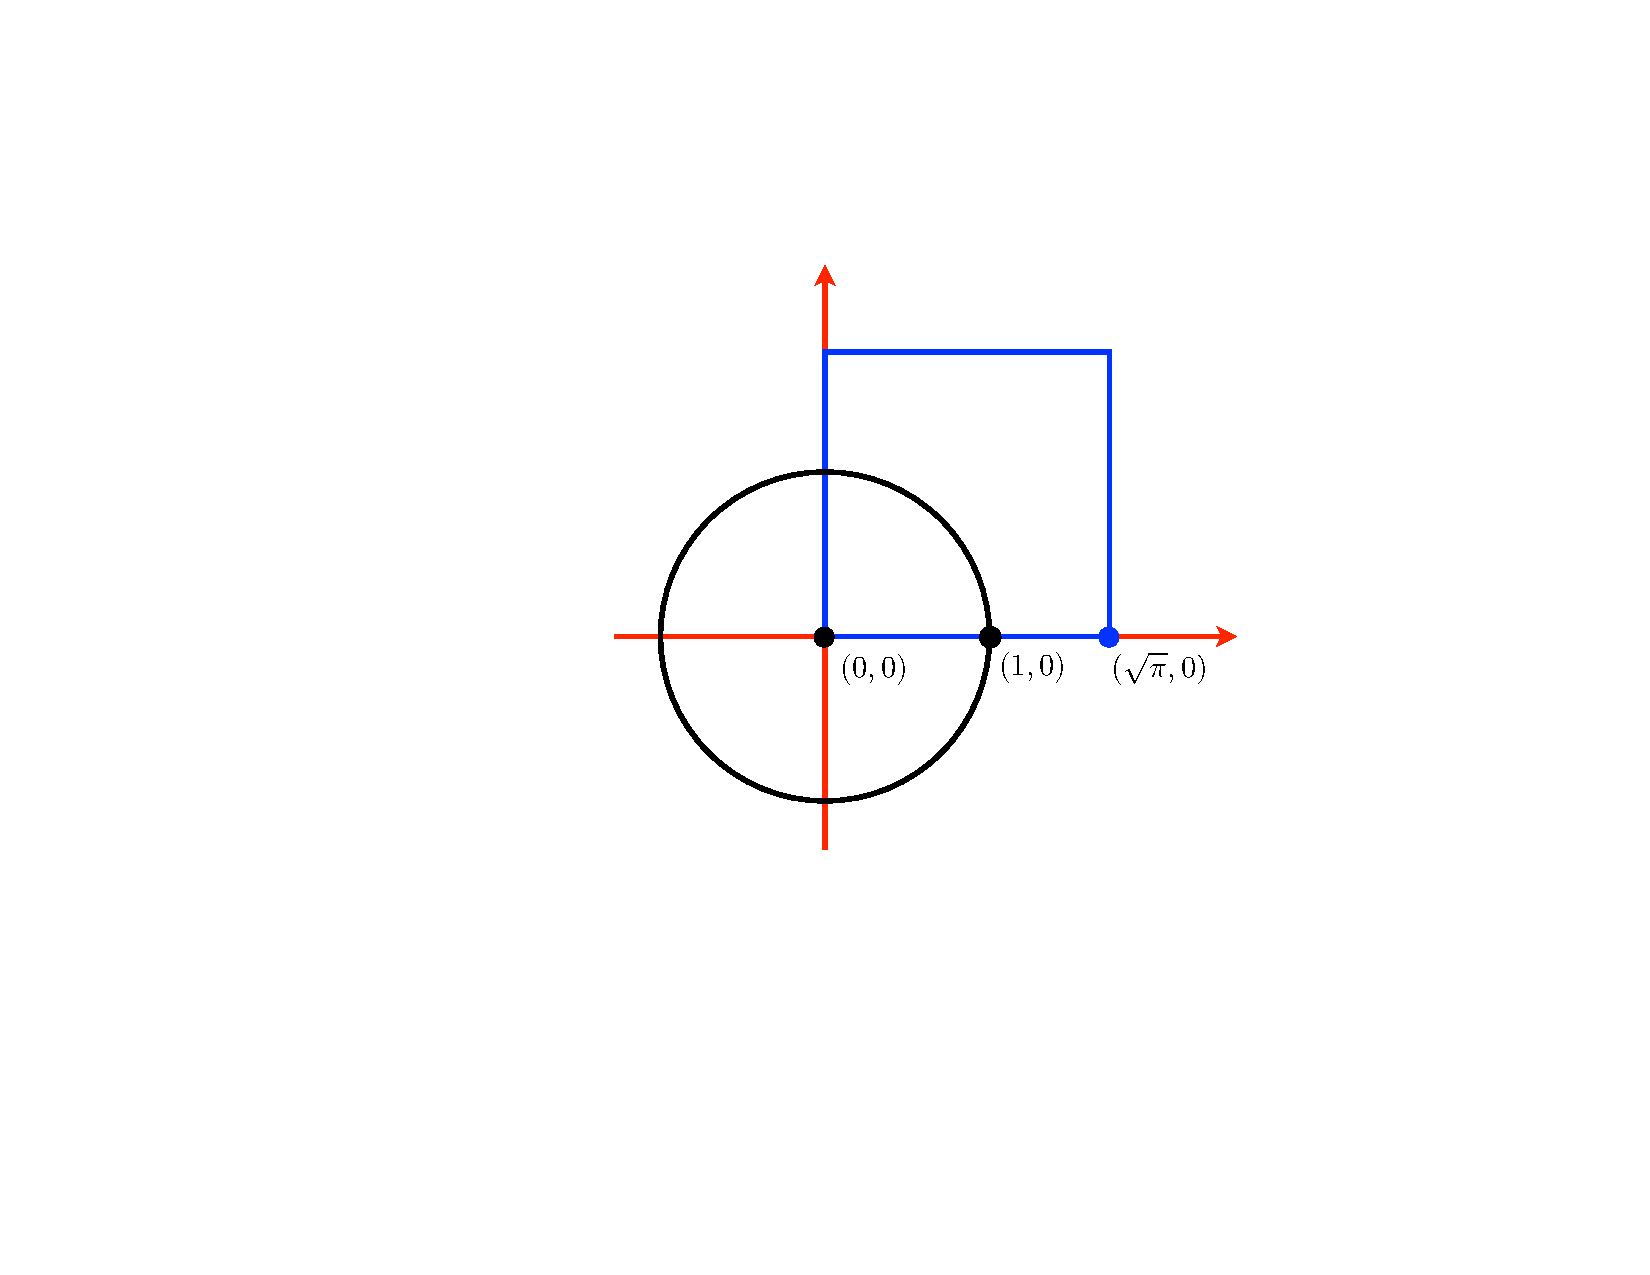
\includegraphics[width=2.5in]{pictures/circle_squaring.pdf}
\end{figure}



\vs\vs

\textbf{2) Doubling of a cube.}  We can assume that two vertices of the front face of the cube 
have coordinates $(0, 0)$ and $(1, 0)$. Doubling of this cube amounts to constructing the point 
with coordinates $( ^{3}\!\!\!\sqrt{2}, 0)$

\begin{figure}[h]
\centering
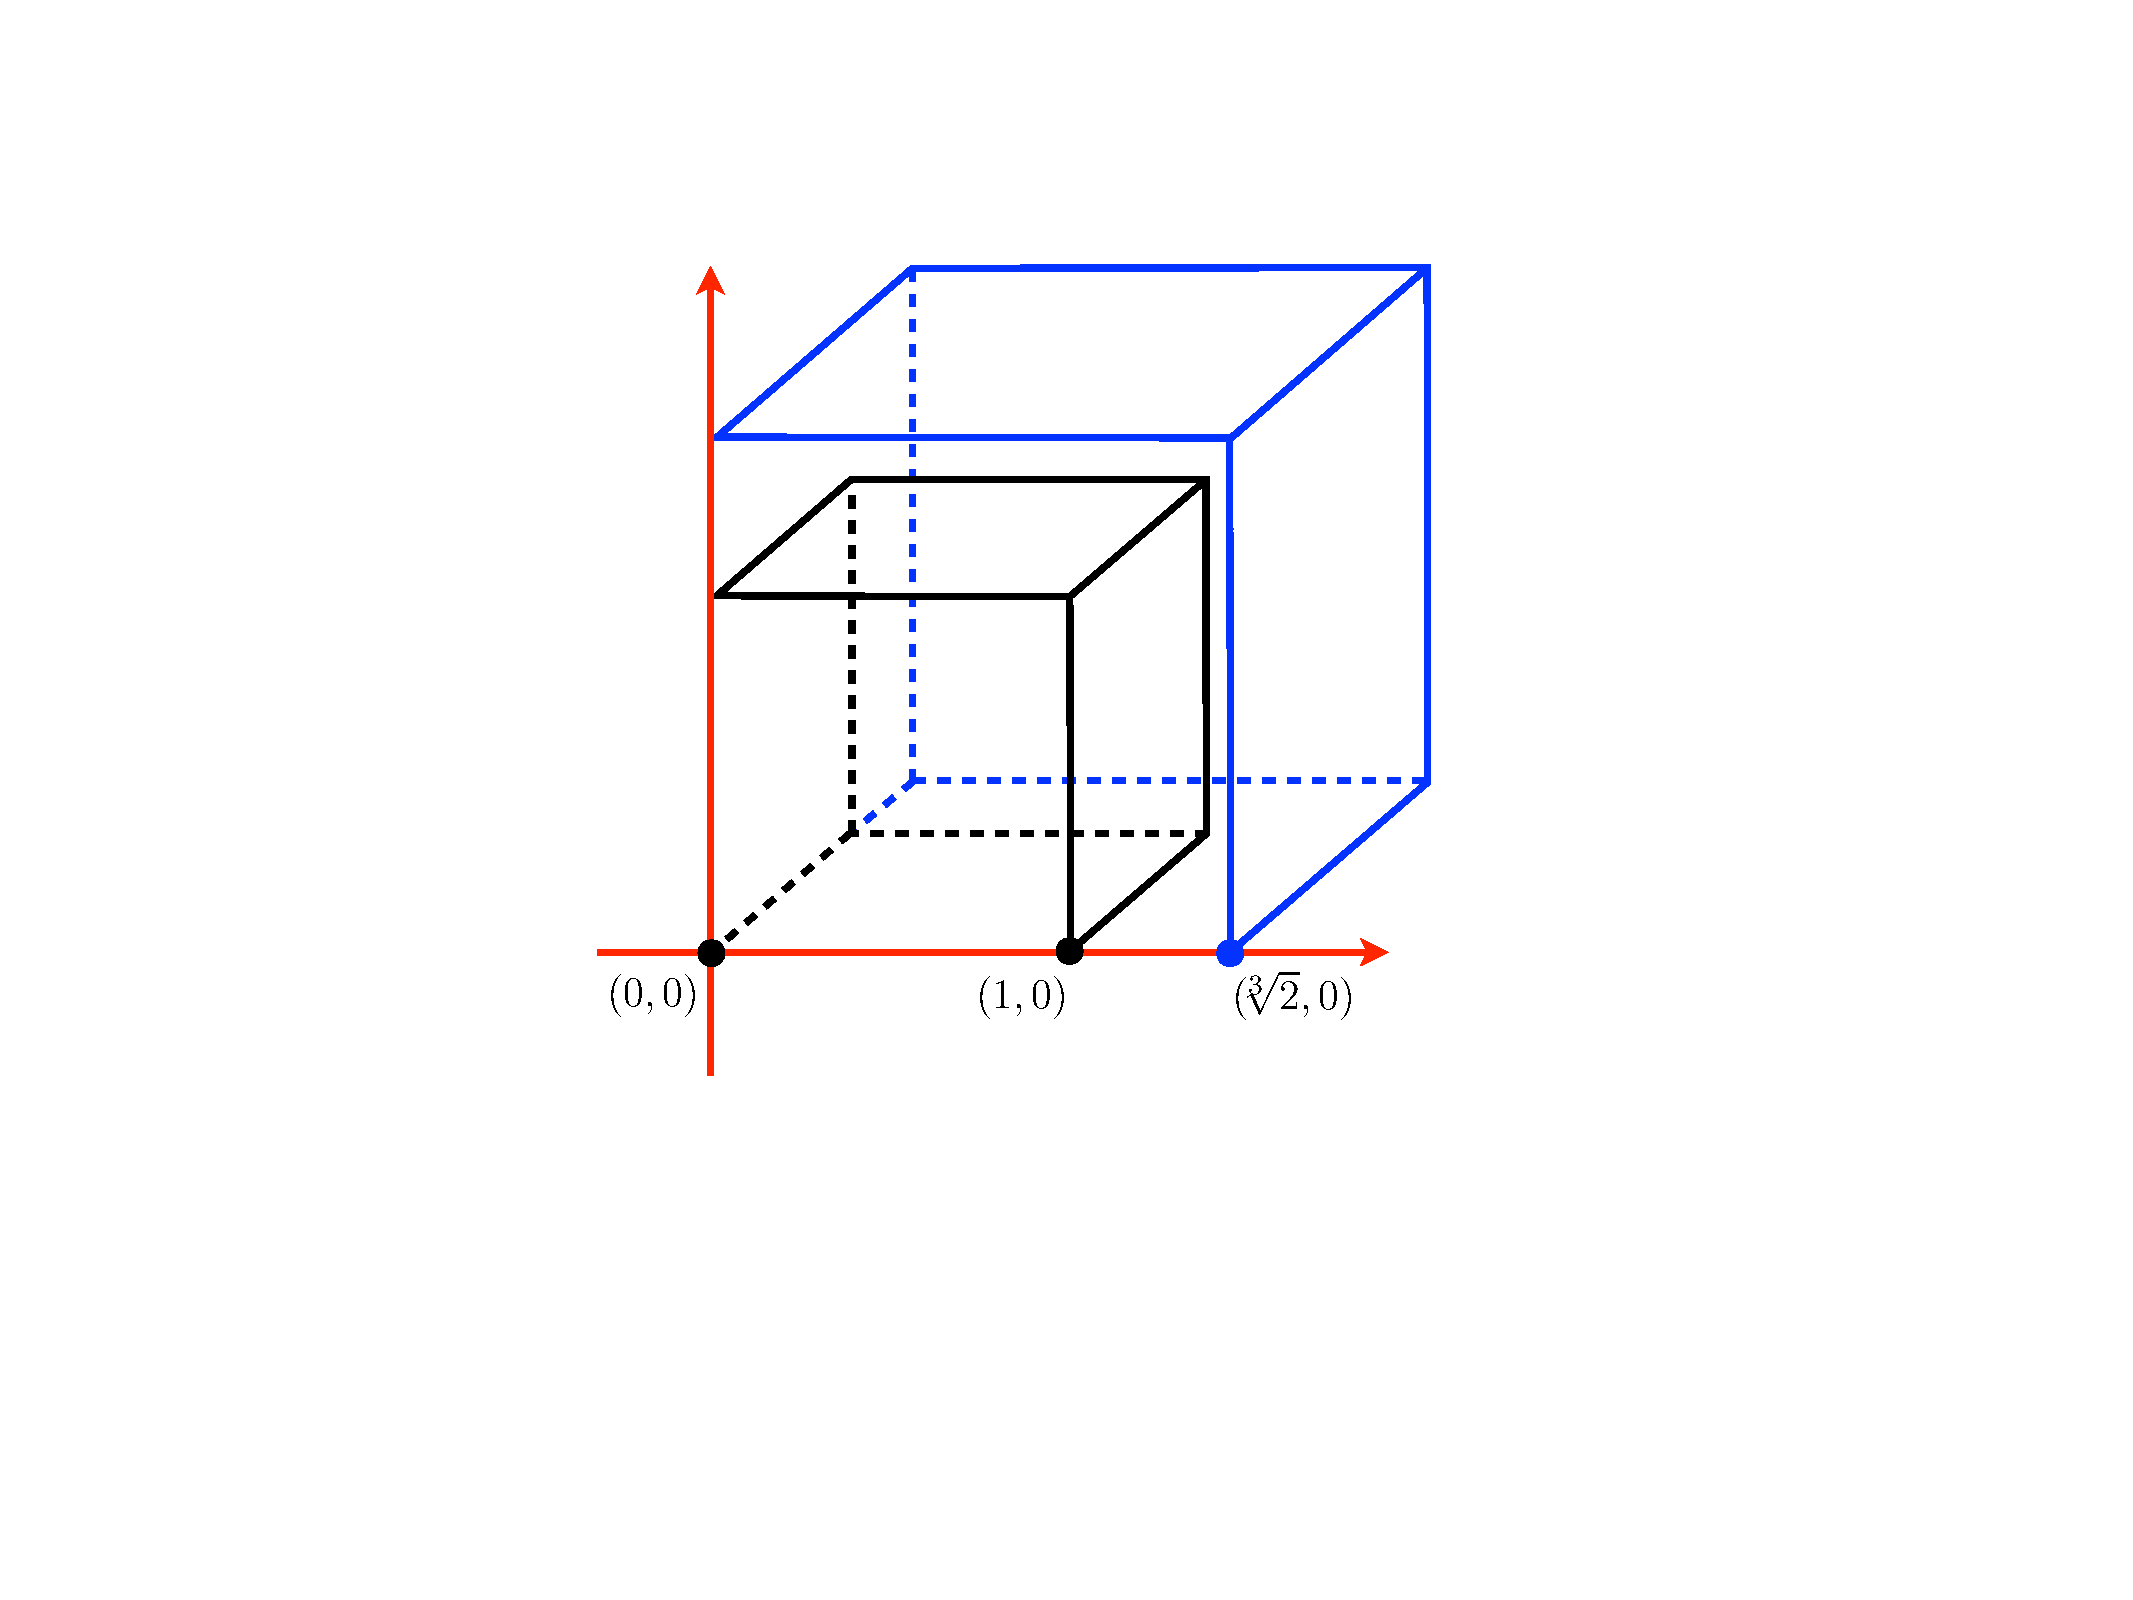
\includegraphics[width=2.5in]{pictures/cube_double.pdf}
\end{figure}



\vs\vs\vs\vs

\ 

\textbf{3) Trisection of an angle.} We can assume that one of the arms of the given 
angle $\theta$ coincides with the $x$-axis. Being given such an angle is equivalent to being 
given the point with coordinates $( \cos \theta, 0)$. Trisection of this angle is equivalent 
to constructing the point with coordinates $( \cos \frac{1}{3}\theta, 0)$

\vs

\begin{figure}[h]
\centering
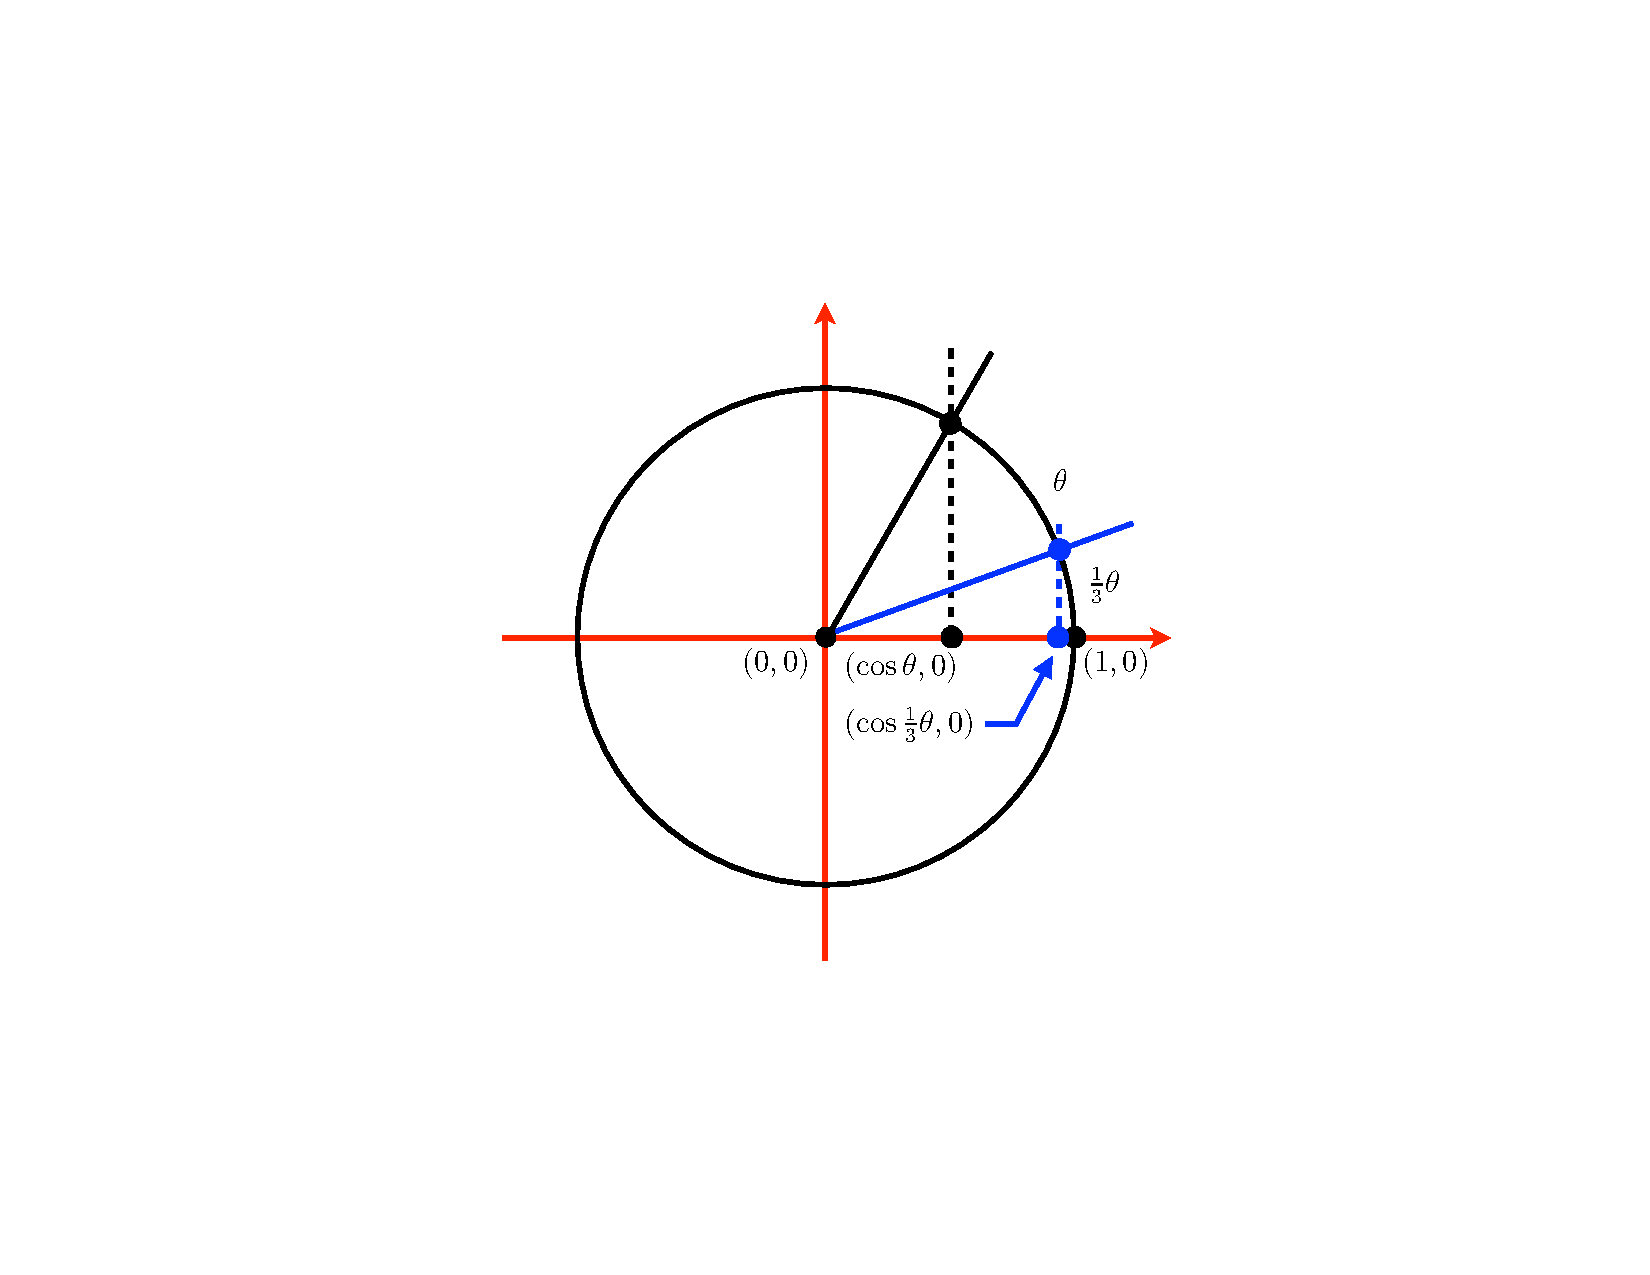
\includegraphics[width=2.8in]{pictures/angle_trisection.pdf}
\end{figure}



\vs\vs\vs\vs


\begin{nn}\textbf{General constructibility problem.}
Assume that on the coordinate plane $\R^{2}$ we are given points a set of points 
$$S_{0} = \{ P_{1}, \dots, P_{n}\}$$
where $P_{i}= (a_{i}, b_{i})$. Assume also that $(0, 0), (1, 0)\in S_{0}$.
We can perform two operations:

\vskip -13mm

\ 
\bit
\item draw a line through any two points in $S_{0}$
\item draw a circle with the center in one point of $S_{0}$ and passing through another 
point of $S_{0}$. 
\eit

\vskip -3mm

Let $S_{1}$ be the set of all intersection points of these lines and circles. 
Recursively, for each $k\geq 1$ let $S_{k}$ be the set of all points obtained 
in this way from the set $S_{k-1}$. Denote
$$S = \bigcup_{k=0}^{\infty} S_{k}$$
\end{nn}

\vs

\begin{definition}
A point $Q\in \R^{2}$ is \emph{constructible from the set $S_{0}$} if $Q\in S$.  
A point $Q\in \R^{2}$ is \emph{constructible} if it is constructible from the set 
$\{(0, 0), (1, 0)\}$.
\end{definition}

\textbf{Problem.} Given a set $S_{0}\in \R^{2}$ determine which points of $\R^{2}$ 
are constructible from $S_{0}$. 



\vs\vs


\begin{note} \ 

\textbf{1)} Squaring of the circle can be performed if the point $(\sqrt{\pi}, 0)$ is constructible. 

\textbf{2)} Doubling of a cube can be performed if the point $( ^{3}\!\!\!\sqrt{2}, 0)$ 
is constructible. 

\textbf{3)} Trisection of the angle $\theta$ can be performed if the point $(\cos \frac{1}{3}\theta, 0)$
is constructible from the set $\{(0, 0), (1, 0), (\cos\theta, 0)\}$. 

\end{note}


\newpage


\textbf{Constructible points and radical extensions.}

\begin{definition}
A field extension $L/K$ is a \emph{degree $2$ radical extension}  if there exist elements 
$a_{1}, \dots, a_{n}\in L$ such that $L = K(a_{1}, \dots, a_{n})$ and for every $i=1, \dots, n$
we have
$$a_{i}^{2}\in K(a_{1}, \dots, a_{i-1})$$  
\end{definition}


\vs\vs


\begin{theorem}
\label{THM_CONSTRUCTIBILITY}
Let $S_{0} = \{P_{1}, \dots, P_{n}\}$ be set of points in $\R^{2}$ where $P_{i} = (a_{i}, b_{i})$.
Let
$$K = \Q(a_{1}, b_{1}, \dots, a_{n}, b_{n})$$
A point $Q = (c, d)$ is constructible from the set $S_{0}$ iff there exists a degree $2$ 
radical extension $L/K$, $L\subseteq \R$ such that $c, d\in L$. 

In particular a point $Q=(c, d)$ is constructible iff   there exists a degree $2$ 
radical extension $L/\Q$, $L\subseteq \C$ such that $c, d\in L$.
\end{theorem}

\vs

\begin{proof}
Exercise. 
\end{proof}

\vs\vs


\begin{corollary}
\label{COR_CONSTRUCTIBILITY}
Let $S_{0} = \{P_{1}, \dots, P_{n}\}$ be a set of points in $\R^{2}$ where $P_{i} = (a_{i}, b_{i})$.
and let
$$K = \Q(a_{1}, b_{1}, \dots, a_{n}, b_{n})$$

If a point $Q= (c, d)$ is constructible  then $[K(c, d): K] = 2^{k}$ for some $k\geq 1$. 
\end{corollary}


\vs 

\begin{proof}
By Theorem \ref{THM_CONSTRUCTIBILITY} we have $K(c, d) \subseteq L$ where 
$L$ is some degree $2$ radical extension of $K$. We have 
$$[L:K] = 2^{m}$$
for some $m\geq 1$, so $[K(c, d):K] = 2^{k}$ for some $1\geq k \geq m$. 

\end{proof}

\vs

\begin{example}  \ 

Since $\sqrt{\pi}$ is a transcendental number thus $\sqrt{\pi}\not\in L$ for any 
degree $2$ radical extension of $\Q$. It follows that the point $(\sqrt{\pi}, 0)$
is not constructible and it is impossible to square a circle using straightedge and 
compass.  
\end{example}

\vs\vs

\begin{example} \ 

We have  $[\Q(^{3}\!\!\!\sqrt{2}): \Q] = 3$. By Corollary \ref{COR_CONSTRUCTIBILITY}
we obtain that the point $( ^{3}\!\!\!\sqrt{2}, 0)$ is not constructible. As a consequence 
it is impossible to double a cube  using straightedge and compass.  

\end{example}


\vs\vs

\begin{example} \ 

Recall that we can perform a trisection of an angle $\theta$ iff the point $(0, \cos \frac{1}{3}\theta)$
can be constructed from the set $S_{0} = \{(0, 0), (1, 0), (\cos\theta, 0)\}$. 
By Theorem \ref{THM_CONSTRUCTIBILITY}  this is possible iff $\cos\frac{1}{3}\theta \in L$
for some degree $2$ radical extension $L$ of the field $K:= \Q(\cos\theta)$. 

\vs 

\emph{Claim.} $\cos\frac{1}{3}\theta \in L$ where $L$ is some degree $2$ radical extension of 
$K$ iff the polynomial 
$$f(x) = x^{3} -\frac{3}{4}x -\frac{1}{4}\cos \theta$$
is not irreducible in $K[x]$. 

Indeed, by de Moivre formula for any angle $\alpha$ we have:
$$\cos 3\alpha = 4 \cos^{3}\alpha -3\cos\alpha$$
It follows from here that $\cos\frac{1}{3}\theta$ is a root of $f(x)$. 

If $f(x)$ is irreducible over $K$ then $[K(\cos\frac{1}{3}\theta):K] =3$,
and so by Corollary  \ref{COR_CONSTRUCTIBILITY} the point $(\cos \frac{1}{3}\theta, 0)$
is not constructible from $S_{0}$. 


Conversely, if $f(x)$ is not irreducible then we have 
$$f(x) = (x-a)g(x)$$
where $a\in K$, $g(x) \in K[x]$, $\deg g(x) =2$. Since $\cos \frac{1}{3}\theta$ is a root 
$f(x)$ we obtain that either $\cos\frac{1}{3}\theta = a$ or $\cos\frac{1}{3}$ is a root of $g(x)$,
and so it can be expressed by elements of $K$ and square roots of such elements.  
In both cases $\cos\frac{1}{3}\theta$ belongs to some degree $2$ radical extension of $K$. 

\vs

Some special cases:

\textbullet \ $\theta = \dfrac{\pi}{4}$

We have $\cos\theta = \frac{\sqrt{2}}{2}$, and so $\Q(\cos \theta) = \Q(\sqrt{2})$. Moreover
$$f(x) = x^{3} -\frac{3}{4}x - \frac{\sqrt{2}}{8}$$
Check: $f(x)$ has a root $-\frac{\sqrt{2}}{2} \in \Q(\sqrt{2})$ so it is not irreducible. Thus 
the angle $\theta = \frac{\pi}{4}$ can be trisected using straightedge and compass. 

\vs

\textbullet \ $\theta = \dfrac{\pi}{3}$

We have $\cos\theta = \frac{1}{2}$, so $\Q(\cos\theta) = \Q$ and 
$$f(x) = x^{3}-\frac{3}{4}x-\frac{1}{8}$$
Check: $f(x)$ has no roots in $\Q$, and so it is irreducible in $\Q[x]$. As a consequence
the angle  $\theta = \frac{\pi}{3}$ cannot be trisected using straightedge and compass. 

\end{example}








%%%%%%%%%%%%%%%%%%%%%%%%%%%%%%%
%%%%%%%%%%%%%%%%%%%%%%%%%%%%%%%
%%%
%%% CONSTRUCTION OF REGULAR POLYGONS
%%%
%%%%%%%%%%%%%%%%%%%%%%%%%%%%%%%
%%%%%%%%%%%%%%%%%%%%%%%%%%%%%%%


\newpage
\section{Construction of regular polygons}
\label{SEC_REGPOLYGONCONSTR}


\textbf{Problem.} For which $n$ it is possible to construct a regular polygon 
with $n$ sides using a  straightedge and a compass?

\vs

\textbf{Note.} Construction of a regular polygon with $n$ sides is equivalent 
to the construction of the  point with coordinates $(\cos \frac{2\pi}{n}, \sin \frac{2\pi}{n})$.

\begin{figure}[h]
\centering
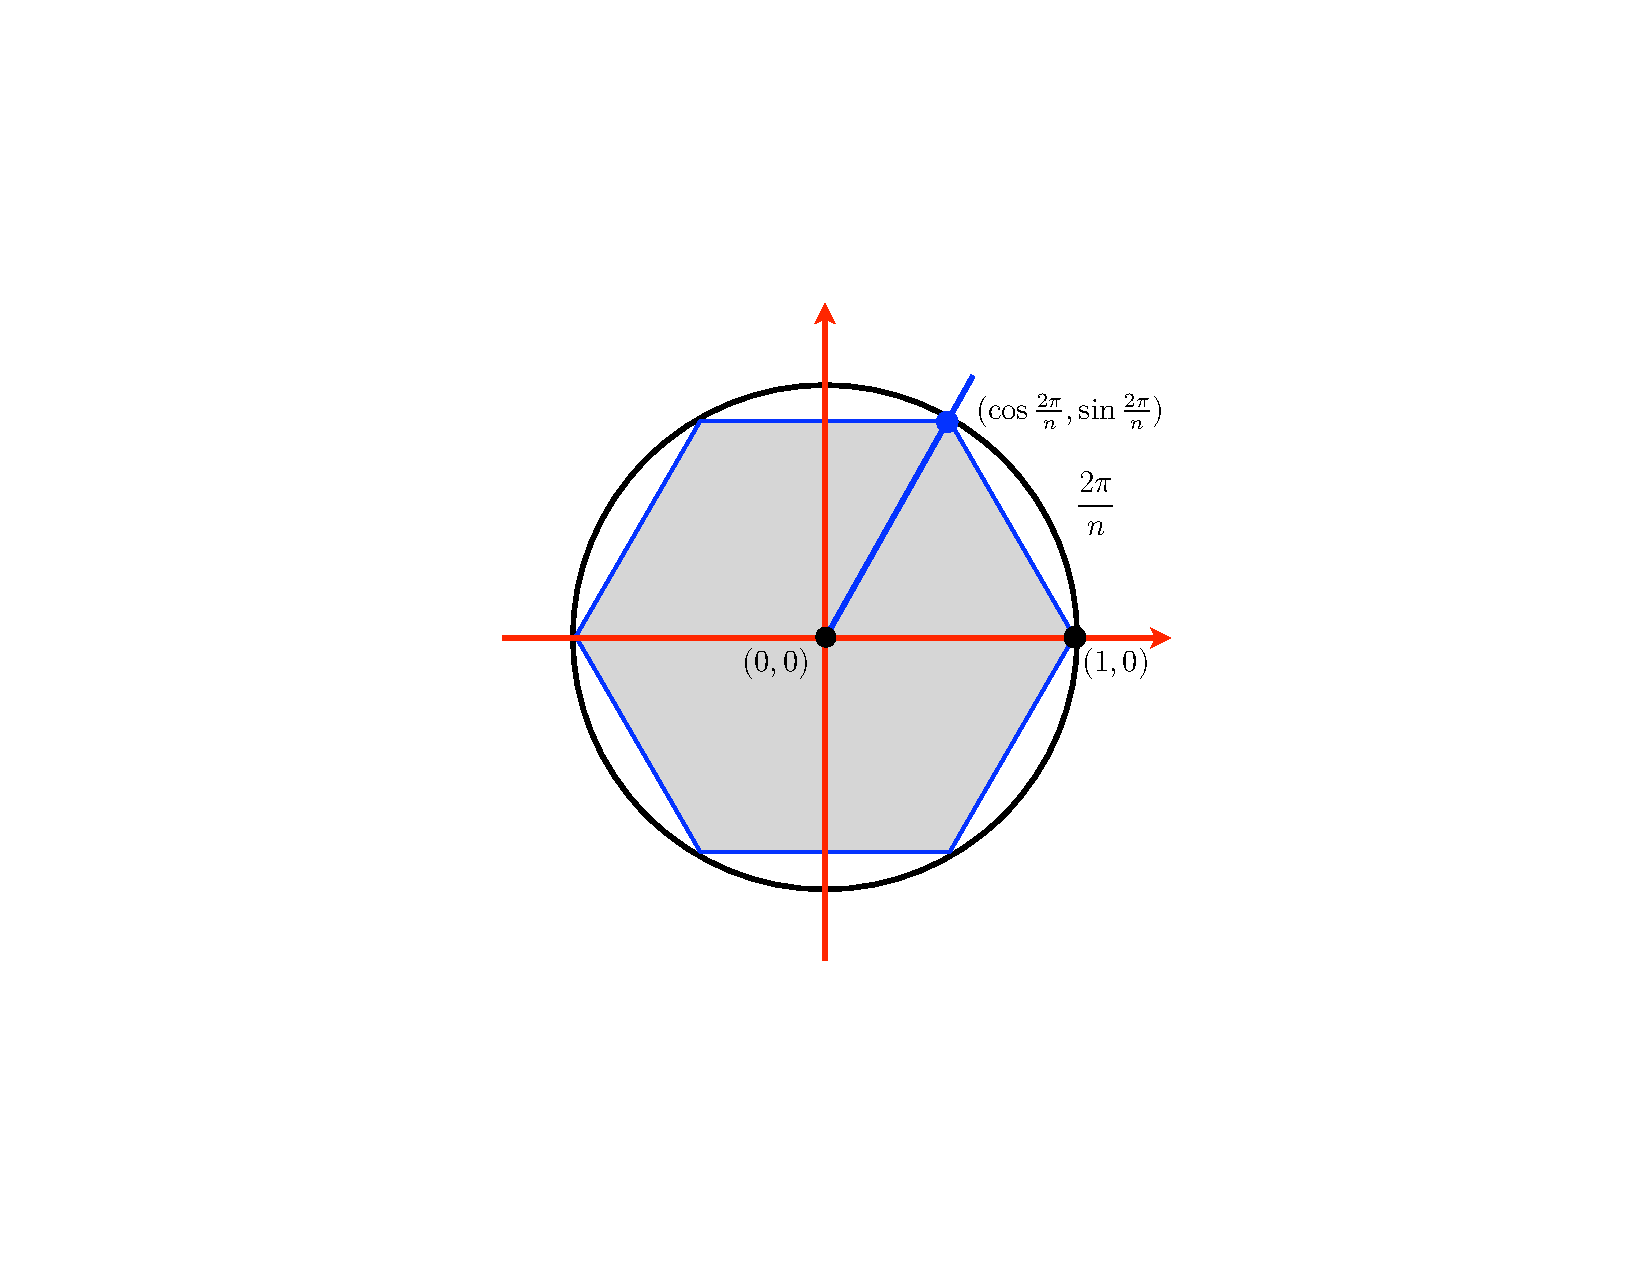
\includegraphics[width=3.2in]{pictures/regular_polygon.pdf}
\end{figure}


\begin{lemma}
The numbers $\cos\frac{2\pi}{n}$,  $\sin\frac{2\pi}{n}$ belong to some degree $2$
radical extension $L$ of $\Q$ iff $\zeta_{n} = \cos\frac{2\pi}{n} + i\sin\frac{2\pi}{n}$
 ome degree $2$ radical extension of $\Q$. 
\end{lemma}

\begin{proof} \ 

($\Rightarrow$) If $\cos\frac{2\pi}{n},   \ \sin\frac{2\pi}{n} \in L$ where $L$ is a degree $2$
radical extension of $\Q$ then $\zeta_{n} \in L(i)$, and $L(i)$ is a degree $2$ radical extension 
of $\Q$. 

\vs 

($\Leftarrow$)  
Assume that $\zeta_{n} \in L$  for some degree $2$ radical extension $L$ of $\Q$. 
We can assume that $i\in L$.
We have $\zeta^{-1} = \cos\frac{2\pi}{n} - i\sin\frac{2\pi}{n}$, which gives
$$\cos\frac{2\pi}{n} = \frac{1}{2}\left(\zeta_{n}+ \frac{1}{\zeta_{n}}\right), \ \ \ \ 
\sin\frac{2\pi}{n} = \frac{1}{2i}\left(\zeta_{n}- \frac{1}{\zeta_{n}}\right)$$
Therefore $\cos\frac{2\pi}{n}, \  \sin\frac{2\pi}{n} \in L$. 

\end{proof}

\vs\vs

\begin{note}
The element $\zeta_{n}$ is a primitive root of unity of degree $n$, so $\Q(\zeta_{n})/\Q$
is the cyclotomic Galois extension of degree $n$ (\ref{DEF_CYCLOTEXT}).  By  
(\ref{NOTE_CYCLOTEXTQ}) we have 
$$\Gal(\Q(\zeta_{n})/\Q)\cong (\Z/n\Z)^{\ast}$$
\end{note}


\vs\vs

\begin{lemma}
If $L/\Q$ is a Galois extension and $[L:\Q] <\infty$ then $L\subseteq M$ for some 
degree $2$ radical extension $M$ iff $\Gal(L/\Q) = 2^{m}$ for some $m\geq 0$
\end{lemma}


\vs 

\begin{proof}
Exercise. 
\end{proof}


\vs\vs

\begin{corollary}
A regular polygon with $n$ sides can be constructed using a straightedge and  a compass
iff $|(\Z/n\Z)^{\ast}| = 2^{m}$ for some $m$. 
\end{corollary}



\vs\vs


\begin{note} \ 

1)\  We have $|(\Z/n\Z)^{\ast}| = \varphi(n)$  where $\varphi(n)$ is the Euler function:
$$\varphi(n) = |\{ m \ | \ 1 \geq m \geq n, \ \ \gcd(m, n) =1 \}|$$

2) \ If $n = p_{1}^{k_{1}}\cdot {\dots}\cdot p_{r}^{k_{r}}$ where $p_{1}, \dots, p_{r}$ are 
distinct primes then 
$$\varphi(n) = \varphi(p_{1}^{k_{1}})\cdot {\dots}\cdot \varphi(p_{r}^{k_{r}})$$
and $\varphi(p_{i}^{k_{i}}) = (p_{i}-1)\cdot p_{i}^{k_{i}-1}$.

\end{note}


\vs\vs

\textbf{Upshot.}  The number $\varphi(n)$ is a power of two iff 
$$n = 2^{k}p_{1}\cdot{\dots}\cdot p_{r}$$
where $p_{1}, \dots, p_{r}$ are distinct primes such that $p_{i} = 2^{m_{i}}+1$
for some $m_{i}\geq 1$. 

\vs\vs

\textbf{Note.} If $2^{m}+1$ is a prime then $m$ must be of the form $2^{s}$ for some $s\geq 0$. 
Prime numbers of the form 
$$F_{s}= 2^{2^{s}}+1$$
are called Fermat primes. 

\vs\vs

We obtain:

\begin{theorem}
A regular polygon with $n$ sides can be constructed using a straightedge and a compass iff 
$$n = 2^{k}p_{1}\cdot{\dots}\cdot p_{r}$$
where $p_{1}, \dots, p_{r}$ are distinct Fermat primes. 
\end{theorem}


\vs\vs

\begin{note}
The only known Fermat primes are 
$$F_{0} =3, \ \ F_{1} =  5, \ \ F_{2} = 17, \ \ F_{3} = 257, \ \  F_{4} = 65537$$
It is not known whether  there are any other prime numbers  of this form.
\end{note} 









%%%%%%%%%%%%%%%%%%%%%%%%%%%%%%%
%%%%%%%%%%%%%%%%%%%%%%%%%%%%%%%
%%%
%%% TRANSCENDENTAL EXTENSIONS
%%%
%%%%%%%%%%%%%%%%%%%%%%%%%%%%%%%
%%%%%%%%%%%%%%%%%%%%%%%%%%%%%%%


\newpage
\section{Transcendental extensions}
\label{SEC_TRANSCEXT}



\begin{definition}
Let $L/K$ be a field extension. A set $S\subseteq L$ is \emph{algebraically independent}
over $K$ if for every finite sequence $(s_{1}, \dots, s_{n})$ of distinct elements of $S$
and for every non-zero polynomial $f(x_{1}, \dots, x_{n})\in K[x_{1}, \dots, x_{n}]$ we have 
$$f(s_{1}, \dots, s_{n}) \neq 0$$
Otherwise we say that the set $S$ is \emph{algebraically dependent} over $K$.  
\end{definition}

\vs\vs

\begin{note}\ 
 If $L/K$ is a field extension then an element $s\in L$ is transcendental over $K$ iff 
the set $S = \{s\}$ is algebraically independent over $K$. 
\end{note}


\vs\vs


\begin{proposition}
\label{PROP_TRANSCVSALGIND}
Let $L/K$ be a field extension. A set $S\subseteq L$ is algebraically independent over $K$ 
iff every  element $s_{0}\in S$ is transcendental over the field $K(S-\{s_{0}\})$.  
\end{proposition}


\vs

\begin{proof} \  

($\Rightarrow$) \ Assume that there exists an element  $s_{0}\in S$ which is algebraic over 
the field $K(S-\{s_{0}\})$. Then there exists a finite subset $\{s_{1}, \dots, s_{n}\}$ such that $s_{0}$
is algebraic over $K(s_{1}, \dots, s_{n})$. Let $0\neq f(x)\in K(s_{1}, \dots, s_{n})[x]$ be a polynomial 
such that $f(s_{0}) = 0$. Notice that  $K(s_{1}, \dots, s_{n})$ is the field of fractions of the ring 
$K[s_{1}, \dots, s_{n}]$. As a consequence we can assume that $f(x)\in K[s_{1}, \dots, s_{n}][x]$:
$$f(x) = f_{r}(s_{1}, \dots, s_{n})x^{r} + {\dots} +  f_{1}(s_{1}, \dots, s_{n})x +  f_{0}(s_{1}, \dots, s_{n})$$
for some $f_{r}, \dots, f_{0} \in K[s_{1}, \dots, s_{n}]$. Take $F\in K[x_{1}, \dots, x_{n}, x_{n+1}]$
given by 
\begin{align*}
F(x_{1}, \dots, x_{n+1})  & =  \\ 
  & f_{r}(x_{1}, \dots, x_{n})x_{n+1}^{r} + {\dots} +  f_{1}(x_{1}, \dots, x_{n})x_{n+1} +  f_{0}(x_{1}, \dots, x_{n}) \\
\end{align*}
\ 

\vskip -13mm

Then $F\neq 0$ and $F(s_{1}, \dots, s_{n}, s_{0}) = 0$. This shows that the set $S$ is not algebraically 
independent over $K$. 

\vs\vs

($\Leftarrow$) \ Assume that the set is not algebraically independent over $K$, and let $n$ be the minimal 
number such that there exists a polynomial $0\neq F\in K[x_{1}, \dots, x_{n}]$  satisfying
$F(s_{1}, \dots, s_{n})=0$ for some distinct elements $s_{1}, \dots, s_{n} \in S$. We have 
\begin{align*}
F(x_{1}, \dots, x_{n})   & =   \\ 
 & f_{r}(x_{1}, \dots, x_{n-1})x_{n}^{r} + {\dots} + 
  f_{1}(x_{1}, \dots, x_{n-1})x_{n} +  f_{0}(x_{1}, \dots, x_{n-1}) \\
\end{align*} 
\ 

\vskip -14mm

for some $f_{r}, \dots, f_{0}\in K[x_{1}, \dots, x_{n-1}]$. Since $F\neq 0$ we must have $f_{i}\neq 0$
for some $0\leq i \leq r$. Then by the minimality of $n$ we have $f_{i}(s_{1}, \dots, s_{n-1})\neq 0$. 
Take $G(x)\in K(s_{1}, \dots, s_{n-1})[x]$ defined by 
\begin{align*}
G(x) =  f_{r}(s_{1}, \dots, s_{n-1})x^{r} 
+ {\dots} + f_{1}(s_{1}, \dots, s_{n-1})x +  f_{0}(s_{1}, \dots, s_{n-1}) \\
\end{align*} 
We have $G(x) \neq 0$ and $G(s_{n}) = F(s_{1}, \dots, s_{n}) = 0$. Therefore $s_{n}$ is 
an algebraic element over $K(s_{1}, \dots, s_{n-1})$, and so it is also algebraic over 
$K(S-\{s_{n}\})$. 


\end{proof}



\vs\vs

\begin{note}
If $L=K(x_{1}, \dots, x_{n})$ is the field of rational functions in variables $x_{1}, \dots, x_{n}$
with coefficients in $K$ then the set $S= \{x_{1}, \dots, x_{n}\}$ is algebraically independent over $K$. 
\end{note}


\vs\vs

\begin{proposition}
If $L/K$ is a field extension and $S= \{s_{1}, \dots, s_{n}\}$ is an algebraically independent 
set over $K$ then we have an isomorphism 
$$K(x_{1}, \dots, x_{n}) \cong K(s_{1}, \dots, s_{n})$$
\end{proposition}

\vs

\begin{proof}
Define $\varphi \colon K(x_{1}, \dots, x_{n}) \to K(s_{1}, \dots, s_{n})$ by
$$\varphi\left(\frac{f(x_{1}, \dots, x_{n})}{g(x_{1}, \dots, x_{n})}\right) = 
\frac{f(s_{1}, \dots, s_{n})}{g(s_{1}, \dots, s_{n})}$$
Check that this an isomorphism of fields. 
\end{proof}



\vs\vs


\begin{definition}
Let  $L/K$ be a field extension. A transcendence basis of the extension $L/K$ is a set $S\subseteq L$
such that 

\vskip -13mm

\ 
\benu
\isep[0]
\item $S$ is algebraically independent over $K$
\item if  $S'\subseteq L$ is an algebraically independent set such that $S\subseteq S'$ then 
$S= S'$. 
\eenu
 
\end{definition}


\vs\vs

\begin{proposition}
For any field extension $L/K$  there exists a transcendence basis of $L/K$. 
\end{proposition}


\vs

\begin{proof}
Exercise. 
\end{proof}


\vs\vs


\begin{theorem}
\label{THM_TRANSCBASISALGEXT}
Let $L/K$ be a field extension. A subset $S\subseteq L$ is a transcendence basis of $L/K$
iff   $S$ a set algebraically independent over $K$ and $L/K(S)$ is an algebraic extension. 
\end{theorem}

\vs\vs

\begin{lemma}
\label{LEMMA_UNIONALGINDEP}
Let $L/K$ be a field extension. If $S, T\subseteq L$ are sets such that $S$ is algebraically 
independent over $K$ and $T$ is algebraically independent over $K(S)$ then $S\cup T$
is algebraically independent over $K$. 
\end{lemma}


\vs


\begin{proof}
Let $s_{1}, \dots, s_{m}\in S$, $t_{1}, \dots, t_{n}\in T$ be distinct elements, and let 
$$0\neq F\in K[x_{1}, \dots, x_{m}, y_{1}, \dots, y_{n}]$$
We need to show that $F(s_{1},\dots,  s_{m}, t_{1}, \dots, t_{n}) \neq 0$
We have 
$$F = \sum_{i_{1}, \dots, i_{n}}f_{i_{1}, \dots, i_{n}}y_{1}^{i_{1}}\cdot{\dots}\cdot y_{n}^{i_{n}}$$
for some $f_{i_{1}, \dots, i_{n}}\in K[x_{1}, \dots, x_{m}]$. Since $F\neq 0$ we have 
$f_{i_{1}, \dots, i_{n}}\neq 0$ for some $i_{1}, \dots i_{n}$, and so by the algebraic independence
of the set $S$ over $K$ we get that $f_{i_{1}, \dots, i_{n}}(s_{1}, \dots, s_{m})\neq 0$. As a consequence 
the polynomial 
$$G(y_{1}, \dots, y_{m}) = 
 \sum_{i_{1}, \dots, i_{n}}f_{i_{1}, \dots, i_{n}}(s_{1}, \dots, s_{m})y_{1}^{i_{1}}\cdot{\dots}\cdot y_{n}^{i_{n}}$$
is a non-zero polynomial in $K(S)[y_{1}, \dots, y_{n}]$. By the algebraic independence of 
the set $T$ over $K(S)$ we obtain
$$F(s_{1}, \dots , s_{m}, t_{1}, \dots, t_{n}) = G(t_{1}, \dots, t_{n})\neq 0$$
\end{proof}


\vs\vs

\begin{proof}[Proof of Theorem \ref{THM_TRANSCBASISALGEXT}] \ 

($\Rightarrow$) Let  $S$ be a transcendence basis of $L/K$. It is enough 
to show that any element $a\in L - K(S)$ is  algebraic over $K(S)$. 

Assume by contradiction that  
$a$ is transcendental over $K(S)$. Then the set $\{a\}$ is algebraically  independent 
over $K(S)$, and so, by Lemma  \ref{LEMMA_UNIONALGINDEP} the set $S\cup \{a\}$
is algebraically independent over $K$. This is impossible since $S$ is a proper subset of 
$S\cup \{a\}$. 


\vs

($\Leftarrow$) Assume that $S$ is a set  algebraically independent over $K$ and that $L/K(S)$
is an algebraic extension. It is enough to show that for any $a\in L - S$ the set 
$S\cup \{a\}$ is not algebraically independent over $K$. 

Assume, by contradiction, that for some $a\in L-S$ the set $S\cup\{a\}$ is 
algebraically independent over $K$. By Proposition \ref{PROP_TRANSCVSALGIND}
we would have then that $a$ is a transcendental element over $K(S)$. This  contradicts 
the assumption that all elements of $L$ are algebraic over $K(S)$. 
\end{proof}


\vs\vs

\begin{definition}
A field extension $L/K$ is \emph{purely transcendental} if $L = K(S)$ where $S\subseteq L$ 
is a set algebraically independent over $K$. 
\end{definition}


\vs\vs

\begin{corollary}
\label{COR_FIELDEXTDECOMP}
For any field extension $L/K$ there exists an intermediate field $K\subseteq M\subseteq L$
such that $M/K$ is a purely transcendental extension and $L/M$ is an algebraic extension. 
\end{corollary}


\vs

\begin{proof}
By Theorem \ref{THM_TRANSCBASISALGEXT} is it enough to take $M = K(S)$ where 
$S\subseteq L$ is a transcendence basis of $L/K$. 
\end{proof}

\vs\vs

\begin{proposition}
If $L/K$ is a field extension and $L= K(A)$ for some set $A\subseteq L$ then  there
exists  $S\subseteq A$ such that $S$ is a transcendence basis of $L/K$.  
\end{proposition}

\vs 

\begin{proof}
By Zorn's Lemma \ref{LEMMA_ZL} we can find a maximal subset $S\subseteq A$ that is 
algebraically independent over $K$. We will show $S$ is a transcendence basis of $L/K$. 


By Theorem \ref{THM_TRANSCBASISALGEXT} it suffices to show that $L/K(S)$ is an 
algebraic extension. Since $L = K(A) = K(S)(A-S)$ this amounts to showing that every 
element $a\in A-S$ is algebraic over $K(S)$. 

Assume, by contradiction, that there exists an element $a\in A-S$ that is transcendental over $K(S)$. 
Then the set $\{a\}$ is algebraically independent over $K(S)$, and so by 
Lemma \ref{LEMMA_UNIONALGINDEP} the set $S\cup \{a\}\subseteq A$ is algebraically independent 
over $K$. This however is impossible  by the maximality of $S$.  
\end{proof}

\vs\vs

\begin{proposition}
\label{PROP_COMPTRANSCBASIS}
If If $K\subseteq L \subseteq M$ are field extensions,  
$S\subseteq L$ be a transcendence basis of $L/K$ and
$T\subseteq M$ be a transcendence basis of $M/L$ then $S\cup T$
is a transcendence basis of $M/K$.
\end{proposition}

\vs

\begin{proof}
The set  $T$ is algebraically independent over $L$, so it is also algebraically independent 
over $K(S)\subseteq L$. By Lemma \ref{LEMMA_UNIONALGINDEP} it follows that 
the set $S\cup T$ is algebraically independent over $K$. 

By Theorem \ref{THM_TRANSCBASISALGEXT} the field $L$ is an algebraic 
extension of $K(S)$.  It follows that $L(T)$ is an algebraic extension of 
$K(S)(T) = K(S\cup T)$ (check!).  Moreover, by Theorem \ref{THM_TRANSCBASISALGEXT} 
again,  $M$ is an algebraic extension of $L(T)$. As a consequence 
$M$ is an algebraic extension of $K(S\cup T)$.  Applying Theorem 
\ref{THM_TRANSCBASISALGEXT} one more time we get from here that $S\cup T$
is a transcendence basis of $M$ over $K$. 
\end{proof}

\vs\vs


\begin{corollary}
If $L/K$ is a field extension and $S\subseteq L$ is a set algebraically independent over 
$K$ then there exists a transcendence basis $S'$ of $L/K$ such that $S\subseteq S'$.  
\end{corollary}

\begin{proof}
The set $S$ is a transcendence basis of the extension $K(S)/K$.  Let $T$ be a transcendence 
basis of the extension $L/K(S)$. By Proposition  \ref{PROP_COMPTRANSCBASIS} 
$S\cup T$ is a transcendence  basis of $L/K$. Therefore we can take $S'= S\cup T$. 
\end{proof}

\vs\vs

\begin{theorem}
If  $L/K$ is a field extension then any two transcendence bases of $L$ over $K$ 
have the same  cardinality. 
\end{theorem}

\vs

\begin{proof}
See Hungerford Theorem 1.8 and Theorem 1.9. 
\end{proof}


\vs\vs

\begin{definition}
The \emph{transcedence degree} of  a field extension $L/K$  is  the cardinality 
of a transcendence basis of $L$ over $K$. It is denoted by $\tr(L/K)$. 
\end{definition}

\vs\vs

\begin{proposition}
If $K\subseteq L \subseteq M$ are field extensions then 
$$\tr(M/K) = \tr(L/K) + \tr(M/L)$$
\end{proposition}


\vs

\begin{proof}
Let $S\subseteq L$ be a transcendence basis of $L/K$  and let 
$T\subseteq M$ be a transcendence basis of $M/L$ over $L$.
By Proposition \ref{PROP_COMPTRANSCBASIS} the set $S\cup T$
is a transcendence basis of $M/K$. Since  $S\cap T = \varnothing$ we obtain 
$$\tr(M/K) = |S\cup T| = |S|+ |T| = \tr(L/K) + \tr(M/L)$$



\end{proof}






%%%%%%%%%%%%%%%%%%%%%%%%%%%%%%%
%%%%%%%%%%%%%%%%%%%%%%%%%%%%%%%
%%%
%%% ALGEBRAIC SETS
%%%
%%%%%%%%%%%%%%%%%%%%%%%%%%%%%%%
%%%%%%%%%%%%%%%%%%%%%%%%%%%%%%%


\newpage
\section{Algebraic sets}
\label{SEC_ALGSETS}

\begin{definition}
Let $K$ be an algebraically closed field, and let 
$$K^{n} = \underbrace{K \times {\dots} \times K}_{n \text{ times}}$$
A subset $A\subseteq K^{n}$ is an \emph{algebraic set} if 
$A$ is the set of solution of some system of polynomial equations


\vskip -5mm

\ 
$$
\begin{cases}
\ f_{1}(x_{1}, \dots, x_{n})  = 0 \\
\  \ \vdots    \\
\ f_{r}(x_{1}, \dots, x_{n})  = 0 \\
\end{cases}
$$

for some $f_{1}, \dots, f_{r}\in K[x_{1}, \dots, x_{n}]$. In such case we write:
$$A = V(f_{1}, \dots, f_{r})$$
\end{definition}

\vs\vs

\begin{note}
 Every finite subset $A= \{a_{1}, \dots, a_{m}\} \subseteq K$ is an algebraic set 
since this is the set of solutions of the equation 
$$(x-a_{1})\cdot{\dots}\cdot(x-a_{m}) = 0$$
\end{note}


\vs\vs

\begin{note}
Different sets of equations may give the same algebraic set. Take e.g. 
$f_{1}, f_{2}, g_{1}, g_{2}\in K[x_{1}, x_{2}]$ given by:
$$f_{1}(x_{1}, x_{2}) = x_{1}, \ \ \ f_{2}(x_{1}, x_{2}) = x_{2}, \ \ \ 
g_{1}(x_{1}, x_{2}) = x_{1}+x_{2}, \ \ \ g_{2}(x_{1}, x_{2}) = x_{1}-x_{2}$$
Then 
$$V(f_{1}, f_{2}) = V(g_{1}, g_{2}) = \{(0, 0)\} \subseteq K^{2}$$
\end{note}



\vs\vs

\begin{definition}
Let $K$ be a field and let $I$ be an ideal of $K[x_{1}, \dots, x_{n}]$. Denote:
$$V(I) := \{(a_{1}, \dots, a_{n}) \ |  \ f(a_{1}, \dots, a_{n}) = 0 \text{ for all } f\in I \}$$
\end{definition}

\vs\vs

\begin{proposition}
\label{PROP_VIVF}
Let $K$ be a field,  let $f_{1}, \dots, f_{r} \in K[x_{1}, \dots, x_{n}]$, and let 
$I = \subgp{f_{1}, \dots, f_{r}}$ be the ideal generated by 
$f_{1}, \dots f_{r}$. Then 
$$V(I) = V(f_{1}, \dots, f_{r})$$
 \end{proposition}
 
 \vs
 
 \begin{proof}
Since $\{f_{1}, \dots, f_{r}\} \subseteq I$ we have $V(I) \subseteq V(f_{1}, \dots, f_{r})$. 

Conversely, assume that  $(a_{1}, \dots, a_{n})\in V(f_{1}, \dots, f_{r})$. If $g\in I$ then 
we have
$$g = \sum_{i=1}^{r}h_{i}f_{i}$$
for some $g_{i}\in K[x_{1}, \dots, x_{n}]$. Therefore 
$$g(a_{1}, \dots, a_{n}) = \sum_{i=1}^{r} g_{i}(a_{1}, \dots, a_{n})f_{i}(a_{1}, \dots, a_{n}) = 0$$
Therefore  $(a_{1}, \dots, a_{n})\in V(I)$, and as a consequence $V(f_{1}, \dots, f_{r}) \subseteq V(I)$.  
 \end{proof}
 
 \vs\vs
 
 \begin{corollary}
 If $K$ is a field, $f_{1}, \dots, f_{r}, g_{1}, \dots, g_{s} \in K[x_{1}, \dots, x_{n}]$ and 
 $$\subgp{f_{1}, \dots, f_{r}} = \subgp{g_{1}, \dots, g_{s}}$$
 then $V(f_{1}, \dots, f_{r}) = V(g_{1}, \dots, g_{s})$. 
 \end{corollary} 
 



%%%%%%%%%%%%%%%%%%%%%%%%%%%%%%%
%%%%%%%%%%%%%%%%%%%%%%%%%%%%%%%
%%%
%%% HILBERT BASIS THEOREM
%%%
%%%%%%%%%%%%%%%%%%%%%%%%%%%%%%%
%%%%%%%%%%%%%%%%%%%%%%%%%%%%%%%


\newpage
\section{Hilbert basis theorem}
\label{SEC_HILBBASTHM}


Goal:

\begin{theorem}
\label{POLYRINGISNOETH}
If $K$ is a field and $I\lhd K[x_{1}, \dots, x_{n}]$ then the ideal $I$ is finitely generated:
$$I = \subgp{f_{1}, \dots, f_{r}}$$
for some $f_{1}, \dots, f_{r}\in K[x_{1}, \dots, x_{n}]$
\end{theorem}

\vs\vs

\begin{note}
Let $K$ be an algebraically closed set. If $I\lhd K[x_{1}, \dots, x_{n}]$ and 
$I = \subgp{f_{1}, \dots, f_{r}}$ then  by Proposition \ref{PROP_VIVF} we have 
$$V(I) = V(f_{1}, \dots, f_{r})$$
i.e. $V(I)$ is an algebraic set. Thus by Theorem \ref{POLYRINGISNOETH} we obtain an 
epimorphism: 
$$
V\colon
\begin{pmatrix}
\text{ ideals} \\[1mm]
\text{  $I\lhd  K[x_{1}, \dots, x_{n}]$} \\
\end{pmatrix}
\ \ \lra \ \ 
\begin{pmatrix}
\text{algebraic sets} \\[1mm]
\text{ $A\subseteq K^{n}$} \\
\end{pmatrix}
$$
\end{note}
which sends an ideal $I$ to the algebraic set  $V(I)$. 


\vs\vs


\begin{definition}
Let $R$ be a commutative ring with identity. The ring $R$ is a \emph{Noetherian ring} 
if every ideal  $I\lhd R$ is finitely generated:
$$I = \subgp{r_{1}, \dots, r_{n}}$$
for some $r_{1}, \dots, r_{n}\in R$. 
\end{definition}

\vs\vs

\begin{example} If $R$ is a PID then $R$ is a Noetherian ring. In particular 

\vskip -13mm

\ 
\benu
\isep[0]
\item $\Z$ is Noetherian 
\item If $K$ is a field then $K[x]$ is Noetherian. 
\eenu
\end{example} 


\vs\vs

\begin{theorem}
\label{THM_NOETHRINGEQCON}
Let $R$ be a commutative ring with identity. The following conditions are equivalent. 

\vskip -13mm

\benu
\item $R$ is a Noetherian ring.
\item If 
$$I_{1}\subseteq I_{2}\subseteq I_{3} \subseteq \dots$$
is any increasing sequence of ideals of $R$ then there exists $n\geq 1$ such
that $I_{n} = I_{m}$ for all $m\geq n$.  
\item Every family of ideals of $R$ contains a maximal element. 
\eenu
\end{theorem}


\vs\vs

\begin{note}
The condition 2) is called the \emph{ascending chain condition} on ideals of $R$. 
\end{note}

\vs\vs


\begin{proof}[Proof of Theorem \ref{THM_NOETHRINGEQCON}]\ 

1) $\Rightarrow$ 2) \  Let  $I_{1}\subseteq I_{2}\subseteq I_{3} \subseteq \dots$
be a chain of ideals in $R$. Take 
$$I := \bigcup_{k=1}^{\infty} I_{k}$$
Then $I$ is an ideal of $R$, and since $R$ is a Noetherian ring this $I = \subgp{r_{1}, \dots, r_{n}}$
for some $r_{1}, \dots, r_{n}\in R$. For  $j=1, \dots, n$ there exists $k_{j}$ such that $r_{j}\in I_{k_{j}}$. 
Take 
$$n= \max\{k_{1}, \dots, k_{n}\}$$
For any  $m\geq n$ we have $r_{1}, \dots, r_{n}\in I_{n}$ and so 
$$I\subseteq I_{m} \subseteq I$$
As a consequence  for any $m\geq n$ we get  $I_{n} = I = I_{m}$. 

\vs


2) $\Rightarrow$ 3) \  Let  $\mathcal{J} $ be a family of ideals in $R$. 
Assume that $\mathcal{J}$ does not contain a maximal element.  Take any $I_{1}\in \mathcal{J}$. 
Since $I_{1}$ is not a maximal element of $\mathcal{J}$ therefore there exists $I_{2}\in \mathcal{J}$
such that $I_{1}\subset I_{2}$ and $I_{1}\neq I_{2}$. By induction we can find in $\mathcal{J}$
an infinite sequence of ideals 
$$I_{1}\subset I_{2} \subset I_{3} \subset \dots $$ 
such that  $I_{k}\neq I_{k+1}$ for all $k\geq 1$. 
This  however contradicts the assumption that ideals of $R$
satisfy the ascending chain condition. 

\vs

3) $\Rightarrow$ 2) \ Let $I$ be an ideal of $R$. We need to show that $I$ is finitely
generated. 

Let $\mathcal{J}$ be the family of all finitely generated ideals $J$ such that
$J\subseteq I$. By assumption $\mathcal{J}$ contains a maximal element 
$J_{0} = \subgp{r_{1}, \dots, r_{n}}$. Assume the $J_{0}\neq I$ and let $s\in I-J_{0}$. 
Then $J_{1} := \subgp{r_{1}, \dots, r_{n}, s}$ is an ideal such that $J_{1}\in \mathcal{J}$, 
$J_{0}\subseteq J_{1}$, and $J_{0}\neq J_{1}$. This is impossible 
since $J_{0}$  is a maximal element of $\mathcal J$. As a consequence we get that 
$I = J_{0}$, and so $I$ is fintely generated.  

\end{proof}

\vs\vs


\begin{HBT}
\label{THM_HBT}
Let $R$ be a commutative ring with identity. If $R$ is a Noetherian ring then $R[x]$
is also Noetherian. 
\end{HBT}

\vs


\begin{proof}
Let $I\lhd R[x]$. We will show that $I$ is generated by a finite set. 

Let $I_{n}\subseteq R$  be the set such that $a\in I_{n}$ if  either 
$a=0$ or if there exists $f(x) = a_{n}x^{n} + \dots + a_{1}x+a_{0}$ such that $f(x)\in I$ and 
$a=a_{n}$.  Check: $I_{n}\lhd R$. Moreover we have 
$$I_{0}\subseteq I_{1}\subseteq \dots$$
Since $R$ is a Noetherian ring we obtain:

\vskip -13mm

\ 
\benu
\item  for any $n\geq 0$ there exists $a_{n,1}, \dots, a_{n, m_{n}}\in R$ such that
$$I_{n} = \subgp{a_{n,1}, \dots, a_{n, m_{n}}}$$
\item there exists $N\geq 0$ such that $I_{N} = I_{N+1} = \dots$.
\eenu

By the definition of $I_{n}$ for any $0\leq n\leq N$ and $1\leq i \leq m_{n}$ there exists 
a polynomial $f_{n, i}(x)\in I$ such that $f_{n, i}(x) = a_{n, i}x^{n} + \dots$.  Define 
$$S:= \{ f_{n, i}(x) \ | \ 0\leq n \leq N, \ \ 1\leq i \leq m_{n} \}$$
Notice that $S$ is a finite set and $S\subseteq I$. 
We will show that $I = \subgp{S}$. 

It suffices to show that  if $g(x)\in I$ then $g(x)\in \subgp{S}$. 
We will argue by  induction with respect to the degree of $g(x)$. 


If $\deg g(x) = 0$ then $g(x) = b_{0}$ for some $b_{0}\in I_{0}$. Then 
$$b_{0} = \sum_{i=1}^{m_{0}} r_{i}a_{0, i}$$
for some $r_{i}\in R$. Since $f_{0, i}(x) = a_{0, i}$ this gives 
$$g(x) = \sum_{i=1}^{m_{0}} r_{i}f_{0, i}(x) $$   
and so $g(x)\in \subgp{S}$. 


Next, assume that for some $n > 0$ if $h(x) \in I$ and $\deg h(x) \leq n-1$ then $h(x)\in \subgp{S}$. 
Let $g(x)\in I$ be a polynomial of degree  $n$:
$$g(x) = b_{n}x^{n} + \dots b_{1}x + b_{0}$$
Assume first that $n\leq N$
By the definition of $I_{n}$ we have $b_{n}\in I_{n}$, and so 
$$b_{n} = \sum_{i=1}^{m_{n}} r_{i}a_{n, i}$$
for some $r_{i}\in R$. 
Define
$$f(x) := \sum_{i=1}^{m_{n}} r_{i}f_{n, i}(x)$$
Notice that  $f(x) = b_{n}x^{n} + \dots$, and so $\deg (g(x)-f(x)) < n$. Also, since 
$g(x), f(x) \in I$ we have $g(x)-f(x)\in I$ and thus by the inductive assumption $g(x)-f(x)\in \subgp{S}$. 
Therefore 
$$g(x) = \underbrace{f(x)}_{\in \subgp{S}} + \underbrace{(g(x)-f(x))}_{\in \subgp{S}}$$
is an element of $\subgp{S}$. 


If $n > N$ then $I_{n} = I_{N}$ so we have 
$$b_{n} = \sum_{i=1}^{m_{N}} r_{i}a_{N, i}$$
Then define 
$$f(x) := x^{n-N}\left(\sum_{i=1}^{m_{N}} r_{i}f_{N, i}(x)\right) = b_{n}x^{n} + \dots$$
Then $f(x)\in \subgp{S}$ and $\deg (g(x) - f(x)) < n $. Similarly as before we obtain from 
here that $g(x)\in \subgp{S}$. 


\vs\vs

\begin{corollary}
\label{COR_HBTNVAR}
If $R$ is a Noetherian ring then  the ring $R[x_{1}, \dots, x_{n}]$ is also 
Noetherian for any $n\geq 0$. 
\end{corollary}

\vs 

\begin{proof}
This follows from Theorem \ref{THM_HBT} by induction with respect to $n$. 
\end{proof}

 \vs\vs
 
 \begin{proof}[Proof of Theorem \ref{POLYRINGISNOETH}] \ 

Since $K$ is a field it is a Noetherian ring. Thus we can apply Corollary \ref{COR_HBTNVAR}
 \end{proof}


\end{proof}



%%%%%%%%%%%%%%%%%%%%%%%%%%%%%%%
%%%%%%%%%%%%%%%%%%%%%%%%%%%%%%%
%%%
%%% RADICAL IDEALS
%%%
%%%%%%%%%%%%%%%%%%%%%%%%%%%%%%%
%%%%%%%%%%%%%%%%%%%%%%%%%%%%%%%


\newpage
\section{Radical ideals}
\label{SEC_RADIDEAL}




\begin{note}
Let $K$ be an algebraically closed field. For any subset $X\subseteq K^{n}$
define 
$$J(X) := \{ f\in K[x_{1}, \dots, x_{n}] \ | \ f(a_{1}, \dots, a_{n}) = 0 \text{ for all } (a_{1}, \dots, a_{n})\in X \}$$
Check: $J(X)$ is an ideal of $K[x_{1}, \dots, x_{n}]$. 

We get maps of sets:
$$
V\colon
\begin{pmatrix}
\text{ ideals} \\[1mm]
\text{  $I\lhd  K[x_{1}, \dots, x_{n}]$} \\
\end{pmatrix}
\ \ \rightleftarrows \ \ 
\begin{pmatrix}
\text{algebraic sets} \\[1mm]
\text{ $A\subseteq K^{n}$} \\
\end{pmatrix} \colon J
$$
Notice that 

\vskip -13mm

\ 
\benu
\item if $I, I' \lhd K[x_{1}, \dots, x_{n}]$  and $I \subseteq I'$ then $V(I) \supseteq V(I')$
\item if $A, A'\subseteq K^{n}$ are algebraic sets and  $A\subseteq A'$ then $J(A)\supseteq J(A')$.
\eenu

\end{note}

\vs\vs


\begin{proposition}
\label{PROP_VJAEQA}
If $A\subseteq K^{n}$ is an algebraic set then $V(J(A)) = A$. 
\end{proposition}


\begin{proof}
If $(a_{1}, \dots, a_{n}) \in A$ then $f(a_{1}, \dots, a_{n}) = 0$ for all $f\in J(A)$. Therefore 
$(a_{1}, \dots, a_{n})\in V(J(A))$.  This show that $A\subseteq V(J(A))$. 

On the other hand,  $A$ is an algebraic set, so $A = V(I)$ for some 
$I\lhd K[x_{1}, \dots, x_{n}]$. We have  $I \subseteq J(A)$ which gives 
$$A = V(I) \supseteq V(J(A))$$ 

\end{proof}

\vs\vs

\begin{note}
It is not true that for any ideal $I\in K[x_{1}, \dots, x_{n}]$ we have $J(V(I)) = I$. 
Take e.g. $I = \subgp{x^{2}}\lhd K[x]$. We have 
$$V(I) = \{ a\in K \ | \ a^{2} = 0\} = \{ 0 \}$$  
Then 
$$J(V(I)) = \{ g(x)\in K[x] \ | \ g(0) = 0 \} = \subgp{x}$$
Therefore $J(V(I)) \neq I$. 
\end{note}



\vs\vs

\begin{definition}
Let $R$ be a  commutative ring with identity. An ideal $I\lhd R$ is a \emph{radical ideal} if 
for every $a\in R$ such that $a^{n}\in I$ for some $n\geq 1$ we have $a\in I$.    
\end{definition}


\vs\vs

\begin{proposition}
\label{PROP_JAISRADID}
If $K$ is an algebraically closed field and $A\subseteq K^{n}$ is an algebraic set 
then $J(A)$ is a radical ideal of $K[x_{1}, \dots, x_{n}]$. 
\end{proposition}


\vs

\begin{proof}
Exercise. 
\end{proof}

\vs\vs

\textbf{Goal.} The following maps are inverse bijections of  sets:

$$
V\colon
\begin{pmatrix}
\text{ radical ideals} \\[1mm]
\text{  $I\lhd  K[x_{1}, \dots, x_{n}]$} \\
\end{pmatrix}
\ \ \rightleftarrows \ \ 
\begin{pmatrix}
\text{algebraic sets} \\[1mm]
\text{ $A\subseteq K^{n}$} \\
\end{pmatrix} \colon J
$$









%%%%%%%%%%%%%%%%%%%%%%%%%%%%%%%
%%%%%%%%%%%%%%%%%%%%%%%%%%%%%%%
%%%
%%% INTEGRAL EXTENSIONS OF RINGS
%%%
%%%%%%%%%%%%%%%%%%%%%%%%%%%%%%%
%%%%%%%%%%%%%%%%%%%%%%%%%%%%%%%


\newpage


\begin{framed}
\ \\
\textbf{\ \ Note.} In Sections \ref{SEC_INTEGRALEXT}-\ref{SEC_NOETHNORM}
all rings are commutative rings  with   identity $1\neq 0$. \\
\end{framed}





\section{Integral extensions of rings}
\label{SEC_INTEGRALEXT}


\begin{definition}
Let $R$, $S$ be rings.  We say that $S$ is a ring extension of $R$ if $R$ is a subring 
of $S$. 
\end{definition}

\vs\vs

\begin{notation}
If $R\subseteq S$ is a ring extension and $A\subseteq S$ is a subset of $S$ then 
$R[A]$ is the smallest subring of $S$ such that $R\cup A\subseteq R[A]$. If 
$A$ is a finite set,  $A= \{a_{1}, \dots, a_{n}\}$ then we write 
$$R[A] = R[a_{1}, \dots, a_{n}]$$
\end{notation}

\begin{note}
We have 
$$R[a] = \{ b\in S \ | \ b= r_{0} + r_{1}a + {\dots} r_{k}a^{k} \ \text{ for some } \ r_{0}, \dots, r_{k} \in R \}$$
and $R[a_{1}, \dots, a_{n}] = R[a_{1}, \dots, a_{n-1}][a_{n}]$. 
\end{note}


\vs\vs

\begin{definition}
Let  $R\subseteq S$ be a ring extension. An element $a\in S$ is 
an  \emph{integral element} over $R$ if $a$ is a root of a monic polynomial $f(x)\in R[x]$.  
\end{definition}

\vs\vs

\begin{example} \ 

\vskip -13mm

\ 
\benu
\isep[5]
\item If $K$,  $L$ are fields and  $K\subseteq L$ then an element $a\in L$ is an integral 
element over $L$ iff $a$ is an algebraic element over $K$. 

\item $\sqrt{2}$ is  integral over $\Z$ since it is a root of the monic polynomial 
$f(x) = x^{2}-2 \in\Z[x]$. 


\item  $\frac{1}{2}$ is not integral over $\Z$. Indeed, if $f(x)\in \Z[x]$ is a monic polynomial
$$f(x) = x^{n} + a_{n-1}x^{n-1} + {\dots} + a_{0}$$
then 
$$2^{n}f(\tfrac{1}{2}) = \underbrace{1 + 2a_{n-1} + \dots + 2^{n}a_{0}}_{\text{odd}} \neq 0$$
so $f(\frac{1}{2}) = 0$. 
\eenu

\end{example}


\vs\vs

\begin{definition}
Let $R$  be a ring.  An $R$-module  $M$ is \emph{faithful} if for every $0\neq r\in R$ there exists 
$m\in M$ such that $rm\neq 0$.  
\end{definition}


\vs\vs

\begin{theorem}
\label{THM_INTELTEQUIVCOND}
Let $R\subseteq S$ be a ring extension and let $a\in S$. The following conditions are 
equivalent. 

\vskip -13mm

\ 
\benu
\isep[0]
\item  The element $a$ is integral over $R$.
\item  $R[a]$ is a finitely generated $R$-module.
\item There exists $M\subseteq S$ such that $M$ is a a faithful $R[a]$-module  and it  
is finitely generated as an $R$-module.
\eenu

\end{theorem}

\vs\vs

\begin{lemma}
\label{LEMMA_DETM}
Let $S$ be a ring and let $A = (a_{ij})$ be an $n\times n$ matrix with coefficients in $S$. 
If $s_{1}, \dots, s_{n} \in S $ are elements such that 
$$A \begin{bmatrix} s_{1} \\ \vdots \\ s_{n} \end{bmatrix} = 0$$  
then $(\det A)\cdot s_{i} = 0$ for  $i=1, \dots, n$. 
\end{lemma}


\vs

\begin{proof}
See Hungerford  p.354 Exercise 8.
\end{proof}

\vs\vs\vs





\begin{proof}[Proof of Theorem \ref{THM_INTELTEQUIVCOND}] \ 

1) $\Rightarrow$ 2) Since the element $a$  is integral over $R$ there exists 
a monic polynomial $f(x) \in R[x]$ such that $f(0)$. Assume that $\deg f(x) = n$. 

If $b\in R[a]$ then $b = g(a)$ for some $g(x)\in R[x]$.  By (\ref{THM_POLYDIVALGORITHM})
there exists $q(x), r(x)\in R[x]$ such that $\deg r(x) \leq n-1$ and 
$$g(x) = q(x)f(x) + r(x)$$
This gives $g(a) = r(a)$. As a consequence we obtain
\begin{align*}
R[a]  & =   \{ r(a) \  \ |\  \ r(x)\in R[x], \ \ \deg r(x) \leq n-1 \} \\
& = \{  b_{0} + b_{1}a + {\dots}  + b_{n-1}a^{n-1} \ \ | \ \ b_{1}, \dots, b_{n-1}\in R \}
\end{align*}
Therefore the elements $1, a, \dots,  a^{n-1}$ generate $R[a]$ as an $R$-module. 

\vs

2) $\Rightarrow$ 3)  $R[a]$ is a faithful $R[a]$-module and by assumption it is finitely generated 
as an $R$-module. Thus we can take $M = R[a]$. 


\vs

3) $\Rightarrow$ 1)  Assume that the set $\{s_{1}, \dots s_{n}\}$ generates $M$ as an $R$-module. 
For every $i= 1, \dots n$ there exists $a_{i, j}\in R$ such that 
$$as_{i} = a_{i1}s_{1} + {\dots} + a_{in}s_{n} $$
This gives a system of equations:
\begin{align*}
& (a_{11}-a)s_{1}      +  a_{12}s_{2} +  \dots a_{1n}s_{n}           = 0  \\
& a_{21}s_{1}            +  (a_{22}-a)s_{2} +  \dots a_{2n}s_{n}     = 0 \\
& \vdots                                                                                                \ \vdots \\
& a_{n1}s_{1}         +  a_{n2}s_{2} +  \dots (a_{nn}-a)s_{n}     = 0 \\
\end{align*}
In the matrix notation this gives:
$$((a_{ij})-aI) \begin{bmatrix} s_{1} \\ \vdots \\ s_{n} \end{bmatrix} = 0$$  
By Lemma \ref{LEMMA_DETM} we get 
$$\det((a_{ij})-aI)s_{i}=0$$ 
for $i=1, \dots, n$. 
Since the elements $s_{1}, \dots, s_{n}$ generate $M$ this shows that 
$\det((a_{ij})-aI)m=0$ for all $m\in M$. Furthermore, since $\det((a_{ij})-aI)\in R[a]$ and $M$ is 
a faithful $R[a]$-module we obtain that $\det((a_{ij})-aI) = 0$.

Take $f(x) = \det((a_{ij})-xI)\in R[x]$. This is a monic polynomial and $f(a)=0$. 
This shows that $a$ is an integral element over $R$. 
\end{proof}


\vs\vs

\begin{definition}
A ring extension $R\subseteq S$ is an \emph{integral extension} if every element of $S$
is integral over $R$. 
\end{definition}

\vs\vs

\begin{lemma}
\label{LEMMA_COMPFINGENMOD}
Let $R\subseteq S \subseteq T$ be ring extensions. If $T$ is finitely generated as an
$S$-module and  $S$ is finitely generated as an $R$-module then $T$ is finitely generated as an 
$R$-module.
\end{lemma}

\vs

\begin{proof}
Exercise. 
\end{proof}

\vs\vs

\begin{proposition}
\label{PROP_INTELTSINTEXT}
Let $R\subseteq S$ be a  ring extension and let $a_{1}, \dots, a_{n}\in S $ be elements 
integral over $R$. Then $R[a_{1}, \dots, a_{n}]$ is finitely generated $R$-module and 
it  is an integral extension of $R$. 
\end{proposition}


\vs 


\begin{proof}
We argue by induction with respect to $n$. 

If $n=1$ then $R[a_{1}]$ is finitely generated $R$-module by 
Theorem  \ref{THM_INTELTEQUIVCOND}. Also, if $b\in R[a_{1}]$ then 
$R[a_{1}]$ is a faithful $R[b]$-module.  Using Theorem \ref{THM_INTELTEQUIVCOND}
again we obtain that $b$ is integral over $R$.   

Assume the statement of the proposition holds for some $n$, and let 
$a_{1}, \dots, a_{n+1}\in S$ be elements integral over $R$. Then $a_{n+1}$
is integral over $R[a_{1}, \dots, a_{n}]$, so $R[a_{1}, \dots, a_{n+1}]$ is a finitely 
generated $R[a_{1}, \dots, a_{n}]$-module. By  Lemma \ref{LEMMA_COMPFINGENMOD} 
we obtain that $R[a_{1}, \dots, a_{n+1}]$ is then a finitely generated $R$-module. 

If $b\in R[a_{1}, \dots, a_{n+1}]$ then $R[a_{1}, \dots, a_{n+1}]$ is a faithful $R[b]$ module, 
so by Theorem \ref{THM_INTELTEQUIVCOND} $b$ is integral over $R$. 
\end{proof}


\vs\vs


\begin{corollary}
Let $R\subseteq S$ be a ring extension and let 
$$R_{\text{int}} := \{ a\in S \ | \  a \text{ is integral over } R\}$$
then $R_{\text{int}}$ is a subring of $S$. 
\end{corollary}

\vs

\begin{proof}
Let $a, b\in R_{\text{int}}$. It is enough to show that $a\pm b$, $ab$ are integral elements
over $R$. This holds since $a\pm b$, $ab\in R[a, b]$, and by Proposition  \ref{PROP_INTELTSINTEXT}
$R[a, b]$ is an integral extension of $R$. 
\end{proof}

\vs\vs

\begin{proposition}
\label{PROP_COMPINTISINT}
Let $R\subseteq S \subseteq T$ be ring extensions. If $T$ is an integral extension of $S$ and 
$S$ is an integral extension of $R$ then $T$ is an integral extension of $R$. 
\end{proposition}

\vs

\begin{proof}
It is enough to show that if $b\in T$ then $b$ is integral over $R$. 

Since $b$ is integral over $S$ there exists a monic polynomial $f(x)\in S[x]$
$$f(x) = x^{n} +a_{n-1}x^{n-1} + {\dots} + a_{0}$$
such that $f(b) = 0$. Since $f(x)\in R[a_{n-1}, \dots, a_{0}]$ it follows that $b$ is integral
over $R[a_{n-1}, \dots, a_{0}]$. By Theorem \ref{THM_INTELTEQUIVCOND} 
$R[a_{n-1}, \dots, a_{0}, b]$ is then a finitely generated $R[a_{n-1}, \dots, a_{0}]$-module. 
Also,  since $a_{n-1}, \dots, a_{0}$ are integral over $R$ by Proposition 
\ref{PROP_INTELTSINTEXT} $R[a_{1}, \dots, a_{n-1}]$ is a finitely generated $R$-module. 
Therefore, by Lemma \ref{LEMMA_COMPFINGENMOD} $R[a_{n-1}, \dots, a_{0}, b]$ is 
a finitely generated $R$-module. Since $R[a_{n-1}, \dots, a_{0}, b]$ is a faithful $R[b]$ module 
applying Theorem \ref{THM_INTELTEQUIVCOND}  we get that $b$ is integral over $R$. 

\end{proof}





%%%%%%%%%%%%%%%%%%%%%%%%%%%%%%%
%%%%%%%%%%%%%%%%%%%%%%%%%%%%%%%
%%%
%%% NOETHER NORMALIZATION LEMMA
%%%
%%%%%%%%%%%%%%%%%%%%%%%%%%%%%%%
%%%%%%%%%%%%%%%%%%%%%%%%%%%%%%%


\newpage
\section{Noether Normalization Lemma}
\label{SEC_NOETHNORM}





\begin{NNL}
\label{THM_NOETHNORM}
Let $K\subseteq S$ be a ring extension such that $K$ is a field and $S$ is  
finitely generated over $K$: 
$$S= K[a_{1}, \dots, a_{n}]$$
for some $a_{1}, \dots, a_{n}\in S$. There exists a ring $K\subseteq R \subseteq S$ such that 
$$R\cong K[x_{1}, \dots, x_{m}]$$
for some $m\leq n$ and that $R\subseteq S$ is an integral extension
\end{NNL}

\vs\vs

\begin{note}
Compare this with the decomposition of field extensions into a purely transcendental 
extension and an algebraic extension (Corollary \ref{COR_FIELDEXTDECOMP}).
\end{note}

\vs\vs

\begin{proof}[Proof of Theorem \ref{THM_NOETHNORM}] \ 

We argue by induction with respect to $n$. 

For  $n=1$ we have $S=K[a_{1}]$. Consider the homomorphism 
$$\varphi\colon K[x] \to K[a_{1}]$$
given by $\varphi(f(x)) = f(a)$. This is an epimorphism, so  if $\Ker(\varphi) = \{0\}$
we get that $K[x]\cong K[a_{1}]$, and then we can take $R=S$. 

If $\Ker(\varphi) \neq \{0\}$
then $f(a)= 0$ for some $0\neq f(x)\in K[x]$. Since $K$ is a field we can assume that $f(x)$
is a monic polynomial. It follows that $a$ is an integral element over $K$, and so by 
(\ref{PROP_INTELTSINTEXT}) $S$ is an integral extension of $K$. In this case take $R=K$. 
 
 
 
Next, assume that the statement of the theorem holds for some $n-1$ and let $S= K[a_{1}, \dots, a_{n}]$. 
We have a homomorphism 
$$\varphi\colon K[x_{1}, \dots, x_{n}]\to   K[a_{1}, \dots, a_{n}]$$
given by  $\varphi(f(x_{1}, \dots, x_{n})) = f(a_{1}, \dots, a_{n})$. If $\Ker(\varphi) = \{0\}$ then 
as before we obtain   $K[x_{1}, \dots, x_{n}]\cong K[a_{1}, \dots, a_{n}]$, so we can take 
$R = S$. 


Assume then that there exists $0\neq f\in \Ker(\varphi)$. We have 
$$f(x_{1}, \dots, x_{n}) = \sum_{(i_{1}, \dots, i_{n})\in I} b_{i_{1}, \dots, i_{n}}x_{1}^{i_{1}}\dots x_{n}^{i_{n}}$$ 
for some $0\neq b_{i_{1}, \dots, i_{n}}\in K$. Let $(j_{1}, \dots, j_{n})$ be the element of $I$ that 
is the biggest with respect to the lexicographic order. Since $K$ is a field we can assume that 
$a_{j_{1}, \dots, j_{n}} =1$.  

Take  
$$d = \max \ \{\  i_{k} \ \  | \  \  1 \leq k \leq n, \ (i_{1}, \dots, i_{n}) \in I \ \}$$
and let $h\in K[x_{1}, \dots, x_{n}]$ be a polynomial given by 
$$h(x_{1}, \dots, x_{n}) = f(x_{1}+x_{n}^{d^{n}},  \ x_{2} + x_{n}^{d^{n-1}}, \dots, x_{n-1} + x_{n}^{d}, x_{n})$$


\emph{Claim.}
Consider $h$ as a polynomial of the variable $x_{n}$ with coefficients in the ring $K[x_{1}, \dots, x_{n-1}]$. 
Then $h$ is a monic polynomial. 

Indeed, notice that 
\begin{align*}
h & = 
\sum_{(i_{1}, \dots, i_{n})\in I} b_{i_{1}, \dots, i_{n}} (x_{1}+x_{n}^{d^{n}})^{i_{1}} 
(x_{2}+x_{n}^{d^{n-1}})^{i_{2}}\dots x_{n}^{i_{n}} \\
& = \sum_{(i_{1}, \dots, i_{n})\in I} b_{i_{1}, \dots, i_{n}} 
(x_{n}^{i_{1}d^{n}+i_{2}d^{n-1}+ \dots i_{n}} \ +\  \text{lower powers of } x_{n})
\end{align*}
By the choice of $(j_{1}, \dots, j_{n})$ the highest degree monomial of $h$ is then 
$$b_{j_{1}, \dots, j_{n}} (x_{n}^{j_{1}d^{n}+j_{2}d^{n-1}+ \dots j_{n}})$$
and by assumption $b_{j_{1}, \dots, j_{n}}=1$

\vs\vs

Next, let   $g(x)$ be the polynomial given by 
$$g(x) = h(a_{1}-a_{n}^{d^{n}}, a_{2}-a_{n}^{d^{n-1}}, \dots,  a_{n-1}-a_{n}^{d}, \ x)$$
Notice that 


\vskip -13mm

\ 
\bit
\isep[0]
\item[(i)] $g(x)\in K[a_{1}-a_{n}^{d_{n}}, \dots,  a_{n-1}-a_{n}^{d}][x]$
\item[(ii)] $g(x)$ is a monic polynomial (since $h$ is monic in $x_{n}$) 
\item[(iii)] $g(a_{n})= f(a_{1}, \dots, a_{n}) = 0$ (since $f\in \Ker(\varphi)$)
\eit

Denote $S' := K[a_{1}-a_{n}^{d_{n}}, \dots,  a_{n-1}-a_{n}^{d}]$. 
By (i)-(iii) above we obtain that $a_{n}$ is an integral element over $S'$,
and so $S'[a_{n}] = K[a_{1}, \dots, a_{n}]$ is an integral extension of 
$S'$.  On the other hand $S'$ is generated over $K$ by $n-1$ elements, 
so by the inductive assumption there is a ring 
$$K\subseteq R \subseteq S'$$
such that $R\cong K[x_{1}, \dots x_{m}]$ for some $m\leq n-1$ and that 
$S'$ is an integral extension of $R$.  Consider the extensions 
$$K\subseteq R \subseteq S$$
To finish the proof it is enough to notice that since $R\subseteq S'$ and $S'\subseteq S$
are integral extensions thus,  by Proposition \ref{PROP_COMPINTISINT}, the extension 
$R\subseteq S$ is also integral. 
\end{proof}

\vs\vs

\begin{corollary}
\label{COR_ALGNULLSTELL}
Let $K$ be a field and let $L$ be a finitely generated ring extension of $K$:
$$L = K[a_{1}, \dots, a_{n}]$$
If $L$ is a field then it is an algebraic extension of $K$.  
\end{corollary}

\vs

\begin{proof}
By the Noether Normalization Lemma \ref{THM_NOETHNORM}
there exists a ring $R$ such that $K\subseteq R \subseteq L$, 
$R\cong K[x_{1}, \dots, x_{m}]$ for some $0\leq m\leq n$, and that 
$R\subseteq L$ is an integral extension. 

It is enough to show that $R$ is a field. Indeed, this will imply that 
$m=0$, (i.e. $K=R$),  and that as a consequence  $K\subseteq L$ 
is an integral (and thus algebraic) extension. 


Take $b\in R$. Since $L$ is a field we have $b^{-1}\in L$. We need to show that 
$b^{-1}\in R$.

Since $L$ is an integral extension of $R$ there exists a monic polynomial 
$f(x) = x^{k} + r_{k-1}x^{k-1} + {\dots} + r_{1}x +r_{0}\in R[x]$ such that 
$f(b^{-1})=0$. This gives 
$$b^{-k}  =  - r_{k-1}b^{-(k-1)} - r_{k-2}b^{-(k-2)}{\dots} - r_{1}b^{-1} - r_{0}$$
Multiplying both sides by $b^{k-1}$ we obtain 
$$b^{-1} = -r_{k-1} - r_{k-2}b  - {\dots} - r_{1}b^{k-2} -r_{0}b^{k-1}$$
Since $r_{i}, b\in R$ therefore  $b^{-1}\in R$. 
\end{proof}






%%%%%%%%%%%%%%%%%%%%%%%%%%%%%%%
%%%%%%%%%%%%%%%%%%%%%%%%%%%%%%%
%%%
%%% HILBERT NULLSTELLENSATZ
%%%
%%%%%%%%%%%%%%%%%%%%%%%%%%%%%%%
%%%%%%%%%%%%%%%%%%%%%%%%%%%%%%%


\newpage
\section{Hilbert Nullstellensatz}
\label{SEC_NULLSTELLENSATZ}


\textbf{Recall.} 

\vskip -13mm

\ 
\benu
\isep[5]
\item Let $K$ be an algebraically closed field. We have maps

$$
V\colon
\begin{pmatrix}
\text{ ideals} \\[1mm]
\text{  $I\lhd  K[x_{1}, \dots, x_{n}]$} \\
\end{pmatrix}
\ \ \rightleftarrows \ \ 
\begin{pmatrix}
\text{algebraic sets} \\[1mm]
\text{ $A\subseteq K^{n}$} \\
\end{pmatrix} \colon J
$$
where 
\begin{align*}
V(I) & = \{(a_{1}, \dots, a_{n})\in K^{n} \ | \ f(a_{1}, \dots, a_{n}) = 0  \ \   \forall f\in I \} \\
J(A) &= \{ f\in K[x_{1}, \dots, x_{n}] \ | \ f(a_{1}, \dots, a_{n})=0 \ \ \forall (a_{1}, \dots a_{n})\in A \ \}
\end{align*}

\item For any algebraic set $A\subseteq K^{n}$ we have $V(J(A)) = A$ (\ref{PROP_VJAEQA}). 

\item If  $A\subseteq K^{n}$ is an algebraic set then $J(A)$ is a radical ideal (\ref{PROP_JAISRADID}).
\eenu

\vs\vs

\textbf{Goal.}  If $I\lhd K[x_{1}, \dots, x_{n}]$ is a radical ideal then $J(V(I)) =I$. As a consequence we 
have inverse bijections of sets 
$$
V\colon
\begin{pmatrix}
\text{ radical ideals} \\[1mm]
\text{  $I\lhd  K[x_{1}, \dots, x_{n}]$} \\
\end{pmatrix}
\ \ \rightleftarrows \ \ 
\begin{pmatrix}
\text{algebraic sets} \\[1mm]
\text{ $A\subseteq K^{n}$} \\
\end{pmatrix} \colon J
$$


\vs\vs

\begin{theorem}[Weak Nullstellensatz]
\label{THM_WEAKNULLSTELL}
Let $K$ be an algebraically closed field. If  $I\in K[x_{1}, \dots, x_{n}]$ then 
$V(I) = \varnothing$ iff $I = K[x_{1}, \dots , x_{n} ] $
\end{theorem}



\vs\vs

\begin{note}
If  $I\lhd K[x]$ then $I = \subgp{f(x)}$ 
for some $f(x)\in K[x]$ since $K[x]$ is a PID. This gives 
$$V(I) = \{ a\in K \ | \ f(a) = 0 \}$$
Therefore in the case of a single variable Theorem \ref{THM_WEAKNULLSTELL}
says that a polynomial $f(x) \in K[x]$ has no roots iff $\subgp{f(x)} = K[x]$, 
i.e. iff  $f(x)$ is a non-zero constant polynomial. This property defines algebraically 
closed fields, so in this case Theorem \ref{THM_WEAKNULLSTELL} is tautologically true.
\end{note}



\vs\vs


\begin{proof}[Proof of Theorem \ref{THM_WEAKNULLSTELL}] \ 

If $I = K[x_{1}, \dots, x_{n}]$ then $1\in I$, and so $V(I)= \varnothing$. 

Assume then that $I\neq K[x_{1}, \dots, x_{n}]$. By (\ref{THM_INCINTOMAXID})
there exists a maximal ideal $P$ such that $I\subseteq P$. We have $V(P) \subseteq V(I)$, 
so it will suffice to show that $V(P)\neq \varnothing$. 


Let 
$$\varphi \colon K[x_{1}, \dots , x_{n}] \to K$$
be a ring homomorphism and let $a_{i}= \varphi(x_{i})$ for $i=1, \dots, n$.  
Notice that if $\varphi|_{K} = \id_{K}$ then $\varphi$ is given by 
$$\varphi(f(x_{1}, \dots, x_{n})) = f(a_{1}, \dots, a_{n})$$
Moreover, $(a_{1}, \dots, a_{n})\in V(P)$ iff $P\subseteq \Ker\varphi$. 
This shows that we have a bijection 

$$
\Phi\colon
\begin{pmatrix}
\text{ ring homomorphisms} \\[2mm]
\text{$\varphi \colon K[x_{1}, \dots , x_{n}] \to K$} \\[2mm]
\text{$\varphi|_{K} = \id_{K}, \ P\subseteq \Ker(\varphi)$}
\end{pmatrix}
\lra
\begin{pmatrix}
\text{points} \\[2mm]
\text{ $(a_{1}, \dots, a_{n})\in V(P)$} \\[2mm]
\\
\end{pmatrix}
$$

where $\Phi(\varphi) = (\varphi(x_{1}), \dots, \varphi(x_{n}))$. In order to show that 
$V(P)\neq \varnothing$ is suffices then to prove that there exists a homomorphism 
$\varphi\colon K[x_{1}, \dots, x_{n}] \to K$ satisfying the above conditions. 


 
Take the quotient ring  $K[x_{1}, \dots, x_{n}]/P$ and let 
$$\pi \colon K[x_{1}, \dots, x_{n}] \to K[x_{1}, \dots, x_{n}]/P$$
be the canonical epimorphism. Identifying $a\in K$ with $\pi(a) = a+P$
we get that $\pi|_{K} = \id_{K}$ and we can consider $K[x_{1}, \dots, x_{n}]/P$ 
as a ring extension of $K$. 
This extension is finitely generated:
$$K[x_{1}, \dots, x_{n}]/P  = K[\pi(x_{1}), \dots, \pi(x_{n})]$$
Since $P$ is a maximal ideal $K[x_{1}, \dots, x_{n}]/P$ is a field. 
By Corollary \ref{COR_ALGNULLSTELL} we obtain  that $K[x_{1}, \dots, x_{n}]/P$  
is an algebraic extension of $K$. Since $K$ is an algebraically closed field
this implies that $K[x_{1}, \dots, x_{n}]/P=K$. Therefore we can take 
$\varphi := \pi$. 

\end{proof}


\vs\vs

\begin{corollary}
If $K$ is an algebraically closed field and $P\lhd K[x_{1}, \dots, x_{n}]$ is  a maximal ideal then 
$$P = \subgp{x_{1}-a_{1}, \dots, x_{n}-a_{n}}$$
for some $a_{1}, \dots, a_{n}\in K$.
\end{corollary}


\vs

\begin{proof}
Since $P\neq K[x_{1}, \dots, x_{n}]$ by Theorem \ref{THM_WEAKNULLSTELL} we get 
$V(P) \neq \varnothing$. Let $(a_{1}, \dots, a_{n})\in V(P)$. Denote 
$$I := \subgp{x_{1}-a_{1}, \dots, x_{n}-a_{n}}$$
Notice that the set $V(I) =  \{(a_{1}, \dots, a_{n})\}$. 
Since $V(I) \neq \varnothing$ the ideal $I$ is a proper ideal of $K[x_{1}, \dots, x_{n}]$. 
Also, since $V(I)\subseteq V(P)$ we have $P\subseteq I$. By maximality of $P$ we 
obtain $P= I$. 
\end{proof}



\vs\vs

\begin{definition}
Let $R$ be a commutative ring and let $I\lhd R$. The \emph{radical of $I$} is the ideal 
$$\sqrt{I} = \{ a\in R \ | \ a^{n} \in I \ \ \text{ for some } \  n\geq 1 \}$$
\end{definition}

\vs\vs

\begin{note}
If $I\lhd R$ then $\sqrt{I} = I$ iff $I$ is a radical ideal.
\end{note}

\vs\vs

\begin{theorem}[Hilbert Nullstellensatz]
\label{THM_NULLSTELL}
Let $K$ be an algebraically closed field. If $I\lhd K[x_{1}, \dots, x_{n}]$ then 
$$J(V(I)) = \sqrt{I}$$
In particular if $I$ is a radical ideal then $J(V(I)) = I$.  

\end{theorem}


\vs

\begin{proof}
Since  $J(V(I))$ is a radical ideal and $I\subseteq J(V(I))$ we have $\sqrt{I}\subseteq J(V(I))$. 
It remains to show then that $J(V(I)) \subseteq \sqrt{I}$.

Let $0\neq F\in J(V(I))$. It will be enough to show that $F^{N} \in I$ for some $N\geq 1$. 

Consider the inclusion homomorphism 
$$K[x_{1}, \dots, x_{n}] \hra K[x_{1}, \dots, x_{n}, y]$$
Let  $g := (1-yF) \in K[x_{1}, \dots, x_{n}, y]$ and let $J\lhd K[x_{1}, \dots, x_{n}, y]$ be the
ideal given by the set $I\cup \{g\}$. 

\emph{Claim.} $V(J) = \varnothing$. 

Indeed, assume that $(a_{1}, \dots, a_{n}, b) \in V(J)$. Since $F\in J(V(I))$ we have 
$F(a_{1}, \dots, a_{n}) = 0$. Therefore 
$$g(a_{1}, \dots, a_{n}, b) = 1- bF(a_{1}, \dots, a_{n}) = 1$$
which is a contradiction since $g\in J$. 


By the Weak Nullstellensatz (\ref{THM_WEAKNULLSTELL}) we obtain that 
$J = K[x_{1}, \dots, x_{n}, y]$. This means that there exists $f_{1}, \dots, f_{k}\in I$ and 
$h_{0}, h_{1}, \dots h_{k}\in K[x_{1}, \dots, x_{n}, y]$ such that 
\begin{equation*}
\tag{$\ast$}
gh_{0} + \sum_{i=1}^{k} f_{i}h_{i}  = 1
\end{equation*}
Consider the ring homomorphism 
$$\varphi\colon K[x_{1}, \dots, x_{n}, y]  \to K(x_{1}, \dots, x_{n})$$
such that  $\varphi|_{K} = \id_{K}$, $\varphi(x_{i}) = x_{i}$, $\varphi(y) = \frac{1}{F}$. 
Notice that $\varphi(g) = 1 - \frac{1}{F} F = 0$. Therefore from the equation ($\ast$) we obtain
$$1 = \varphi(1) =  \sum_{i=1}^{k} f_{i}\varphi(h_{i})$$
For $i=1, \dots k$ we have  $h_{i} = \sum_{j=0}^{n_{i}} h_{ij}y^{j}$ 
for some  $h_{ij} \in K[x_{1}, \dots, x_{n}]$. This gives:
$$1 = \sum_{i=1}^{k} f_{i}\varphi(h_{i}) = 
\sum_{i=1}^{k} f_{i}\left( \sum_{j=1}^{n_{i}} h_{ij}\frac{1}{F^{j}}\right)$$
Take $N = \max\{n_{1}, \dots, n_{k}\}$. We obtain
$$F^{N} = F^{N}\left(  \sum_{i=1}^{k} f_{i}\left( \sum_{j=1}^{n_{i}} h_{ij}\frac{1}{F^{j}}\right)\right) 
=  \sum_{i=1}^{k} f_{i}\left( \sum_{j=1}^{n_{i}} h_{ij}F^{N-j}\right)$$
where $N-j \geq 0$. 
Since $f_{i}\in I$ and $h_{ij}F^{N-j} \in K[x_{1}, \dots, x_{n}]$ for all $i, j$ this shows that 
$F^{N}\in I$. 
\end{proof}



\vs\vs

\begin{corollary}
\label{COR_NULLSTELLCORRESP}
Let $K$ be an algebraically closed field. We inverse bijections of sets:
$$
V\colon
\begin{pmatrix}
\text{ radical ideals} \\[1mm]
\text{  $I\lhd  K[x_{1}, \dots, x_{n}]$} \\
\end{pmatrix}
\ \ \rightleftarrows \ \ 
\begin{pmatrix}
\text{algebraic sets} \\[1mm]
\text{ $A\subseteq K^{n}$} \\
\end{pmatrix} \colon J
$$
\end{corollary}

\vs

\begin{proof}
This follows directly from Proposition \ref{PROP_VJAEQA} 
and Theorem \ref{THM_NULLSTELL}.
\end{proof}



\vs\vs

\begin{corollary}
\label{COR_IDEALSDAMEALGSETS}
If $I_{1}, I_{2}\lhd K[x_{1}, \dots, x_{n}]$ then $V(I_{1}) = V(I_{2})$ iff 
$\sqrt{I_{1}} = \sqrt{I_{2}}$. 
\end{corollary}


\vs

\begin{proof}
If $I\lhd K[x_{1}, \dots x_{n}]$ then by (\ref{PROP_VJAEQA}) and (\ref{THM_NULLSTELL})
we have 
$$V(I) = V(J(V(I))) = V(\sqrt{I}) $$
Therefore if $\sqrt{I_{1}} = \sqrt{I_{2}}$ then $V(I_{1}) = V(I_{2})$. 

Conversely, if $V(I_{1}) = V(I_{2})$ then 
$$\sqrt{I_{1}} = J(V(I_{1})) = J(V(I_{2})) = \sqrt{I_{2}}$$

\end{proof}


%%%%%%%%%%%%%%%%%%%%%%%%%%%%%%%
%%%%%%%%%%%%%%%%%%%%%%%%%%%%%%%
%%%
%%% ZARISKI TOPOLOGY
%%%
%%%%%%%%%%%%%%%%%%%%%%%%%%%%%%%
%%%%%%%%%%%%%%%%%%%%%%%%%%%%%%%


\newpage
\section{Zariski topology}
\label{SEC_ZARISKITOP}


\textbf{Recall.} If $R$ is a commutative ring and $I, I\lhd R$ then 
$$I+J := \{a+b \ | \ r\in I, s\in J\}$$ 
In general, if $\{I_{i}\}_{i\in S}$ then 
$$\sum_{i\in S} I_{i} :=  \left\{ \sum_{i\in S} a_{i} \ \ \bigg| \ \ a_{i}\in I_{i}, \  a_{i}\neq 0
\text{ for finitely many $i$ only} \right\}$$
$\sum_{i\in S} I_{i}$ is the smallest ideal of $R$ containing $I_{i}$ for all $i\in S$. 


\vs\vs


\begin{proposition}
\label{PROP_INTERSUMIDEALSVSALGSETS}
Let $K$ be an algebraically closed set. 

\vskip -13mm 

\ 
\benu
\item If $\{I_{1}, \dots, I_{k}\}$ is a finite family of ideals of $K[x_{1}, \dots, x_{n}]$ then 
$$V(I_{1})\cup \dots \cup V(I_{k}) = V(I_{1}\cap \dots \cap I_{k}) $$
\item If $\{I_{i}\}_{i\in S}$ is an arbitrary family of ideals of $K[x_{1}, \dots, x_{n}]$ then 
$$ \bigcup_{i\in S} V(I_{i}) = V({\textstyle{\sum_{i\in S} I_{i}}})$$
\eenu


\end{proposition}


\begin{proof} \ 

1)  Denote $J := I_{1}\cap \dots \cap I_{k}$. Since $J \subseteq I_{i}$ for $i=1,\dots, k$
thus $V(I_{i}) \subseteq V(J) $ and so   
$$ \bigcup_{i=1}^{n} V(I_{i}) \subseteq V(J)$$
Conversely, assume that $a\not\in  \bigcup_{i=1}^{n} V(I_{i})$. Then for $i= 1, \dots, k$
there exists $f_{i}\in I_{i}$ such that $f_{i}(a) = 0$. Take $f = f_{1}\cdot{\dots}\cdot f_{n}$. 
We have $f\in J$,  and $f(a) \neq 0$. Thus $a\not\in V(J)$.  Therefore we obtain
$$ V(J) \subseteq  \bigcup_{i=1}^{n} V(I_{i}) $$


\vs 


2)  Denote $J:= \sum_{i\in S} I_{i}$.
Since $I_{i} \subseteq J$ for all $i\in S$ thus $V(J) \subseteq V(I_{i})$ and so 
 $$V(J) \subseteq \bigcap_{i\in S} V(I_{i})$$
Conversely, if $a\in  \bigcap_{i\in S} V(I_{i})$ then $f(a)=0$ for  all $f\in I_{i}$
Since the set $\bigcup_{i\in S}I_{i}$ generates $J$ we get that $f(a)=0$ for all $f\in J$, 
and so $a\in V(J)$.   

\end{proof}


\vs\vs


\begin{corollary}
\label{COR_ALGSETSARECLOSED}
Let $K$ be an algebraically closed field. 

\vskip -13mm 

\ 
\benu
\item $\varnothing$ and $K^{n}$ are algebraic sets in $K^{n}$.  
\item If $\{A_{1}, \dots A_{n}\}$ is a finite family of algebraic sets in $K^{n}$
then $\bigcup_{i=1}^{n} A_{i}$ is also an algebraic set. 
\item If $\{A_{i}\}_{i\in S}$ is an arbitrary family of algebraic sets in $K^{n}$
then $\bigcap_{i\in S} A_{i}$ is also an algebraic set. 
\eenu
\end{corollary}

\vs

\begin{proof} \ 

1) We have $\varnothing = V(\subgp{1})$ and $K^{n} = V(\{0\})$. 

\vs

2) -- 3)  This follows directly from Proposition \ref{PROP_INTERSUMIDEALSVSALGSETS}.


\end{proof}

\vs\vs


\begin{definition/proposition}
Let $K$ be an algebraically closed field. There exists a topology on $K^{n}$ such that 
closed sets in this topology are algebraic sets $A\subseteq K^{n}$. This topology is called 
the \emph{Zariski topology} on $K^{n}$.  
\end{definition/proposition}

\vs

\begin{proof}
This follows directly from Corollary \ref{COR_ALGSETSARECLOSED}.
\end{proof}

\vs\vs

\begin{note}
A set $A\subseteq K^{1}$ is algebraic iff $A$ is the set of zeros of some polynomial 
$f(x)\in K[x]$. If $f(x) = 0$ then $A= K^{1}$, if $f(x) = 1$, then $A= \varnothing$, and
if $\deg f(x) > 0$ then  $A$ is a finite set. Thus the only closed sets in the Zariski topology 
on $K^{1}$ are $K^{1}$, $\varnothing$ and  all finite subsets $A\subseteq K^{1}$.   
\end{note}



%%%%%%%%%%%%%%%%%%%%%%%%%%%%%%%
%%%%%%%%%%%%%%%%%%%%%%%%%%%%%%%
%%%
%%% IRREDUCIBLE ALGEBRAIC SETS
%%%
%%%%%%%%%%%%%%%%%%%%%%%%%%%%%%%
%%%%%%%%%%%%%%%%%%%%%%%%%%%%%%%


\newpage
\section{Algebraic varieties}
\label{SEC_ALGVARIETIES}

\begin{definition}
Let $K$ be an algebraically closed field. An algebraic set $A\subseteq K^{n}$ is 
\emph{irreducible} if for any algebraic sets $A_{1}, A_{2}\subseteq K^{n}$ satisfying 
$A= A_{1}\cup A_{2}$ we have either $A=A_{1}$ or $A= A_{2}$. 

An irreducible algebraic set is called an \emph{algebraic variety}.
\end{definition}

\vs\vs

\begin{theorem}
\label{THM_ALGSETIRREDDECOMP}
Let $K$ be an algebraically closed field. Every algebraic set in $K^{n}$ is a union 
of a finite number of algebraic varieties. 
\end{theorem}



\vs

\begin{proof}
We argue by contradiction. Let $\mathcal{J}$ be the family of all radical ideals
$I\lhd K[x_{1}, \dots, x_{n}]$  such that $V(I)$ is not a union of 
a finite number of  algebraic varieties. Assume that $\mathcal{J}\neq \varnothing$.  

Since the ring $K[x_{1}, \dots, x_{n}]$ is Noetherian, by 
Theorem \ref{THM_NOETHRINGEQCON} there exists an ideal $J$ that is a 
maximal element in $\mathcal{J}$. The set 
$V(J)$ is not an algebraic variety (since  by the definition of $\mathcal{J}$ it is not a union 
of a finite number of algebraic varieties), so 
$$V(J) = V(I_{1}) \cup V(I_{1})$$ 
for some radical ideals $I_{1}, I_{2}\lhd K[x_{1}, \dots, x_{n}]$. 
such that  $V(I_{1}) \neq V(J) \neq V(I_{2})$. Since $V(I_{i})\subseteq V(J)$ for $i=1,2$ we have 
$J\subseteq I_{i}$. Also, since $V(J)\neq V(I_{i})$  and $J$, $I_{i}$ are radical ideals, thus 
by Corollary \ref{COR_NULLSTELLCORRESP} we have $J\neq I_{i}$ for $i=1, 2$. 
Since $J$ is a maximal element in $\mathcal{J}$ this implies that $I_{1}, I_{2}\not\in \mathcal{J}$. 
As a consequence the sets $V(I_{1})$ and $V(I_{2})$ are finite unions of algebraic varieties. 
Since $V(J) = V(I_{1})\cup V(I_{2})$ this implies that $V(J)$ is also a union of a finite number 
of algebraic varieties which is a contradiction.  

\end{proof}

\vs\vs

\begin{definition}
Let $K$ be an algebraically closed field, let $A\subseteq K^{n}$ be an algebraic set 
and let 
\begin{equation*}
\tag{$\ast$}
A=  A_{1}\cup \dots \cup A_{r}
\end{equation*}
where $A_{1}, \dots, A_{r}$ are algebraic varieties. The decomposition 
($\ast$) is \emph{irredundant} if 
$$A\neq A_{1} \cup \dots \cup  A_{i-1} \cup A_{i+1} \cup \dots \cup A_{r}$$
for all $i=1, \dots, r$. 
\end{definition}

\vs\vs

\begin{theorem}
Let $K$ be an algebraically closed field and let $A\subseteq K^{n}$ be an algebraic set. 
Assume we have two irredundant decompositions of $A$ into  algebraic varieties: 
$$ B_{1}\cup \dots \cup B_{r} \ =\  A \  =\   C_{1}\cup \dots \cup C_{s} $$
Then $s=r$ and there exists a permutation $\sigma \colon \{1, \dots, r\} \to \{1, \dots, r\}$
such that $B_{i} = C_{\sigma(i)}$ for $i=1, \dots, r$. 
\end{theorem}


\vs

\begin{proof}
Let $1\leq i\leq r$.  We have 
$$B_{i} = (B_{i}\cap C_{1})\cup \dots \cup (B_{i}\cap C_{s})$$
and since $B_{i}$ is an algebraic variety  thus 
$B_{i} = B_{i}\cap C_{\sigma(i)}$ for some $1\leq \sigma(i)\leq s$. 
Therefore $B_{i} \subseteq C_{\sigma(i)}$. By the same argument we obtain that 
$C_{\sigma(i)}\subseteq B_{k}$ for some $1\leq k\leq r$. This gives 
$$B_{i}\subseteq C_{\sigma(i)} \subseteq B_{k}$$
Since the decomposition $A= B_{1}\cup \dots \cup B_{r}$ is irredundant  we have  $i=k$, 
and so $B_{i} = C_{\sigma(i)}$. Since the decomposition 
$A = C_{1}\cup \dots \cup C_{s}$ is irredundant the map 
$$\sigma \colon \{1, \dots , r\} \to \{1, \dots , s\}$$
is onto, and in particular $s\leq r$. On the other hand, since the decomposition 
$A= B_{1}\cup \dots \cup B_{r}$ is irredundant  $\sigma $ must be 1-1, and so $r\leq s$. 
As a consequence $r=s$ and $\sigma$ is a bijection. 
\end{proof}

\vs\vs

\begin{theorem}
\label{THM_IRREDALGSETPRIMEID}
Let $K$ be an algebraically closed field.  An algebraic 
set $V\subseteq K^{n}$ is an algebraic variety  iff $J(V)\lhd K[x_{1}, \dots, x_{n}]$ is a prime ideal. 
\end{theorem}

\vs\vs

\begin{lemma}
\label{LEMMA_PRODRADISINTERSRAD}
Let $K$ be an algebraically closed field. If  $I_{1}, I_{2} \lhd K[x_{1}, \dots, x_{n}]$ then  
$$\sqrt{I_{1}I_{2}} = \sqrt{I_{1}\cap I_{2}}$$
As a consequence we have 
$$V(I_{1}I_{2}) = V(I_{1}\cap I_{2}) = V(I_{1}) \cup V(I_{2})$$
\end{lemma}


\vs 

\begin{proof}
Exercise. 
\end{proof}


\vs\vs

\begin{proof}[Proof of Theorem \ref{THM_IRREDALGSETPRIMEID}] \ 

($\Rightarrow$) Assume that $V$ is an algebraic variety, and let $I_{1}, I_{2}\lhd K[x_{1}, \dots, x_{n}]$ 
be ideals such that $I_{1}I_{2}\subseteq J(V)$. By  Proposition \ref{PROP_PRIMEIDPRODCHAR}
it suffices to show that either $I_{1}\subseteq J(V)$ or $I_{2}\subseteq J(V)$.

By Lemma \ref{LEMMA_PRODRADISINTERSRAD} we have 
$$V \subseteq V(I_{1}I_{2}) = V(I_{1}\cap I_{2}) = V(I_{1}) \cup V(I_{2})$$
As a consequence 
$$V=  (V\cap V(I_{1})) \cup  (V\cap V(I_{1}))$$
Since $V$ is a variety we obtain that  either $V= V\cap V(I_{1})$ or $V=V\cap V(I_{2})$. 
We can assume that $V = V\cap V(I_{1})$. This gives $V\subseteq V(I_{1})$, and so 
$I_{1} \subseteq J(V)$. 
 
 \vs

($\Leftarrow$) \ Assume that $J(V)$ is a prime ideal and let
$$V= V_{1}\cup V_{2}$$
where $V_{1}, V_{2}$ are algebraic sets. For $i=1, 2$ let $J_{i} = J(V_{i})$. 
Since $J_{1}$, $J_{2}$  are radical ideals the ideal $J_{1}\cap J_{2}$ is also radical (check).
By Proposition \ref{PROP_INTERSUMIDEALSVSALGSETS} we have 
$$V(J_{1}\cap J_{2}) = V(J_{1}) \cup V(J_{2}) = V_{1}\cup V_{2} = V$$
so the bijective correspondence (\ref{COR_NULLSTELLCORRESP})
implies that  $J(V) = J_{1} \cap J_{2}$.  This in turn gives 
$$J_{1}J_{2}\subseteq J(V)$$
Since  $J(V)$ is a prime ideal by (\ref{PROP_PRIMEIDPRODCHAR}) we have that either 
$J_{1}\subseteq J(V)$ or $J_{2}\subseteq J(V)$. This gives that either $V\subseteq V(J_{1}) = V_{1}$
or $V\subseteq V(J_{2}) = V_{2}$.  Therefore either $V= V_{1}$ or $V= V_{2}$. 


\end{proof}

\vs\vs

\begin{corollary}
Let $K$ be an algebraically closed set.
We have inverse bijections of sets: 
$$
V\colon
\begin{pmatrix}
\text{ prime ideals} \\[1mm]
\text{  $I\lhd  K[x_{1}, \dots, x_{n}]$} \\
\end{pmatrix}
\ \ \rightleftarrows \ \ 
\begin{pmatrix}
\text{algebraic varieties} \\[1mm]
\text{ $A\subseteq K^{n}$} \\
\end{pmatrix} \colon J
$$
\end{corollary}

\vs

\begin{proof}
This follows from Corollary \ref{COR_NULLSTELLCORRESP} and 
Theorem \ref{THM_IRREDALGSETPRIMEID}. 
\end{proof}


\vs\vs


\begin{corollary}
\label{COR_IDISINTEROFPRIMID}
Let $K$ be an algebraically closed field and let $I\lhd K[x_{1}, \dots, x_{n}]$ be 
a radical ideal. Then there exist prime ideals $P_{1}, \dots, P_{m}\lhd K[x_{1}, \dots, x_{n}]$
such that 
$$I= P_{1} \cap \dots \cap P_{n}$$
\end{corollary}

\vs

\begin{proof}
By Theorem \ref{THM_ALGSETIRREDDECOMP} we have 
$$V(I) = V_{1}\cup \dots \cup V_{k}$$
where $V_{1}, \dots, V_{k}$ are algebraic varieties. 
Let $P_{i} = J(V_{i})$. By Theorem \ref{THM_IRREDALGSETPRIMEID} $P_{1}, \dots, P_{n}$
are prime ideals. Since $V_{i} = V(P_{i})$ we obtain 
$$V(I) = V(P_{1}) \cup \dots \cup V(P_{k}) = V(P_{1}\cap \dots \cap P_{k})$$
Both  $I$ and $P_{1}\cap \dots \cap P_{k}$ are radicals ideals so by (\ref{COR_NULLSTELLCORRESP})
we have 
$$I = P_{1}\cap \dots \cap P_{k}$$
\end{proof}


\vs\vs

\begin{corollary}
\label{COR_RADIINTERPRIMEID}
Let $K$ be an algebraically closed field and let $I\lhd K[x_{1}, \dots, x_{n}]$. Then 
$$\sqrt{I} = \bigcap_{i\in S} P_{i}$$
where $\{P_{i}\}_{i\in S}$ is the family of all prime ideals of $K[x_{1}, \dots, x_{n}]$
such that  $I\subseteq P_{i}$. 
\end{corollary}


\vs

\begin{proof}
Since prime ideals are radical ideals, for any prime ideal $P$ such that  $I\subseteq P$ we have
$\sqrt{I} \subseteq P$. Therefore 
$$\sqrt{I} \subseteq \bigcap_{i\in S} P_{i}$$
Conversely, by Corollary \ref{COR_IDISINTEROFPRIMID} there exist ideals 
$P_{i_{1}}, \dots, P_{i_{k}}\in \{P_{i}\}_{i\in S}$ such that  
$\sqrt{I} = P_{i_{1}}\cap \dots \cap P_{i_{k}}$. This gives 
$$\bigcap_{i\in S} P_{i} \subseteq P_{i_{1}}\cap \dots \cap P_{i_{k}} =  \sqrt{I}$$
As a consequence $\sqrt{I} = \bigcap_{i\in S} P_{i} $. 
\end{proof}


\vs\vs

\begin{note} \ 
\label{NOTE_NILRADICAL}
\vskip -13mm

\ 
\benu
\isep[5]
\item The statement of Corollary \ref{COR_RADIINTERPRIMEID} holds if we replace 
$K[x_{1}, \dots, x_{n}]$ by an arbitrary commutative ring with identity (exercise). 

\item As a consequence  for the zero ideal $\{0\}\lhd R$ we obtain that 
$\sqrt{\{0\}}$ is the intersection of all prime ideals of $R$. Notice that we have 
$$\sqrt{\{0\}} = \{a\in R \ | \ a^{k} = 0 \ \text{for some} \ k\geq 0\}$$
The ideal $\sqrt{\{0\}}$ is called the \emph{nilradical} of $R$. We denote:
$$\nil(R):= \sqrt{\{0\}}$$
\eenu
\end{note}






%%%%%%%%%%%%%%%%%%%%%%%%%%%%%%%
%%%%%%%%%%%%%%%%%%%%%%%%%%%%%%%
%%%
%%% REGULAR FUNCTIONS
%%%
%%%%%%%%%%%%%%%%%%%%%%%%%%%%%%%
%%%%%%%%%%%%%%%%%%%%%%%%%%%%%%%


\newpage
\section{Regular functions}
\label{SEC_REGFUNCTIONS}

\begin{definition}
Let $K$ be an algebraically closed field and let $V\subseteq K^{n}$  be an 
algebraic set. A \emph{regular function}  is a function $V \to K$ given by 
 $$(a_{1}, \dots, a_{n}) \mapsto f(a_{1}, \dots, a_{n})$$
 where $f$ is some polynomial in $K[x_{1}, \dots, x_{n}]$. 
\end{definition}


\vs\vs


\begin{note}\ 
\label{NOTE_REGFUNCTIONS}
\vskip -13mm

\ 
\benu
\isep[5]
\item Different polynomials may define the same regular function. E.g. 
if $V = \{0\} \subseteq K^{1}$ then $f(x) = x$ and $g(x) = x^{2}+x$  define 
the same regular function since $f(0) = g(0) = 0$. 
\item Polynomials $f, g\in K[x_{1}, \dots, x_{n}]$ define the same regular function on $V$
iff  for every $a\in V$ we have 
$$f(a)-g(a) = 0$$
Equivalently, $f, g$ define the same regular function on $V$ iff $f-g \in J(V)$. This gives a bijection 
of sets:
$$
\begin{pmatrix}
\text{ regular functions} \\[1mm]
\text{  $V \to K$} \\
\end{pmatrix}
\ \ \rightleftarrows \ \ 
\begin{pmatrix}
\text{elements of the rings} \\[1mm]
\text{ $K[x_{1}, \dots, x_{n}]/J(V)$} \\
\end{pmatrix}
$$

\eenu
\end{note}


\vs\vs

\begin{definition}
Let $K$ be an algebraically closed field and let $V\subseteq$ be an algebraic set. 
The coordinate ring of $V$ is the ring 
$$K[V] := K[x_{1}, \dots, x_{n}]/J(V)$$
\end{definition}

\vs\vs\vs\vs\vs

\begin{note}\ 

\vskip -13mm

\ 
\benu
\item The ring  $K[V]$ is a finitely generated $K$-algebra. 


\item Check: since $J(V)$ is a radical ideal
we have  $\nil(K[V]) = \{0\}$ (see \ref{NOTE_NILRADICAL}).  

\item If $V$ is an algebraic variety then $J(V)$ is a prime ideal and so $K[V]$
is an integral domain. 
\eenu

\end{note}


\vs\vs

\begin{proposition}
Let $K$ be an algebraically closed field. If $A$ is a finitely generated $K$-algebra
such that $\nil(A) = \{0\}$ then  there exists an algebraic set $V$ such that $A= K[V]$. 
Moreover, if $A$ is in integral domain then $V$ is an algebraic variety.
\end{proposition}

\vs

\begin{proof}
Since $A$ is finitely generated we have $A = K[a_{1}, \dots, a_{n}]$
for some elements $a_{1}, \dots, a_{n}\in A$. We have a  ring epimorphism
$$\varphi \colon K[x_{1}, \dots, x_{n}] \to A$$
given by $\varphi(x_{i}) = a_{i}$ for $i=1, \dots, n$ and $\varphi|_{K} = \id_{K}$. 
Take $V := V(\Ker{\varphi})$.  Since $\nil(A) = \{0\}$ thus $\Ker(\varphi)$ is a radical ideal 
(check!) and so by Theorem \ref{THM_NULLSTELL} we have $J(V) = \Ker(\varphi)$. 
Therefore we have 
$$K[V] =  \Ker[x_{1}, \dots, x_{n}]/\Ker{\varphi} \cong A$$
If $A$ is an integral domain then $\Ker(\varphi)$ is a prime ideal and so $V$ is an 
algebraic variety. 

\end{proof}


\vs\vs

\begin{definition}
Let $K$ be an algebraically closed field and let $V\subseteq K^{n}$, $W\subseteq K^{m}$
be algebraic sets. Let $p_{i}\colon W \to K$ be the map given by 
$$p_{i}(a_{1}, \dots, a_{m}) = a_{i}$$
A map
$$\varphi \colon V \to W$$ 
is a \emph{morphism of algebraic sets}  
if $p_{i}\varphi \colon V \to K$ is a regular function for $i=1, \dots, m$.
\end{definition}


\vs\vs

\begin{note}
If $V$ is an algebraic set over $K$ then morphisms $V \to K$ coincide with regular 
functions on $V$ (check).  
\end{note}

\vs\vs


\begin{proposition}
If $K$ is an algebraically closed field and  $\varphi\colon V\to W$, $\psi\colon W \to Z$
are  morphism of algebraic sets over $K$ then $\psi\varphi\colon V\to Z$ is also a morphism 
of algebraic sets.  
\end{proposition}

\vs

\begin{proof}
Exercise. 
\end{proof}


\vs\vs

\begin{definition}
For  an algebraically closed field $K$ denote by $\mathcal{A}lg\mathcal{S}et(K)$ the category 
of algebraic sets over $K$ and morphisms of algebraic sets. 
Let $\mathcal{V}ar(K)$ denote the subcategory of algebraic varieties over $K$. 
\end{definition}

\vs\vs

\begin{note}
Let $K$ be an algebraically closed field and let  $\varphi \colon V \to W$ be a morphism of 
algebraic sets over $K$. For any regular function $f\colon W\to K$ the map
$f\varphi\colon V \to K$ is a regular function on $V$. Using the bijective correspondence 
between regular functions on $W$  and elements of the coefficient ring $K[W]$ we obtain a map 
$$\varphi^{\sharp}\colon K[W] \to K[V]$$
Check: $\varphi^{\sharp}$ is a homomorphism of $K$-algebras. 
\end{note}

\vs\vs

\begin{proposition}
Let $K$ be an algebraically closed field and let $\mathcal{F}\mathcal{D}_{K}$ be the category 
of finitely generated  $K$-algebras that are integral domains. 
The functor
$$F \colon \mathcal{V}ar(K) \to \mathcal{F}\mathcal{D}_{K}$$
given by $F(V) = K[V]$ and $F(\varphi) = \varphi^{\sharp}$ is an equivalence of categories. 
\end{proposition}

%% NOTE: equivalence of categories has not been defined previously...

\vs\vs

\begin{corollary}
If $K$ is an algebraically closed field and $V, W$ are algebraic varieties over $K$ then 
$V\cong W$ in $\mathcal{V}ar(K)$ iff $K[V]\cong K[W]$ as $K$-algebras. 
\end{corollary}




%%%%%%%%%%%%%%%%%%%%%%%%%%%%%%%
%%%%%%%%%%%%%%%%%%%%%%%%%%%%%%%
%%%
%%% SUGGESTED FURTHER READING
%%%
%%%%%%%%%%%%%%%%%%%%%%%%%%%%%%%
%%%%%%%%%%%%%%%%%%%%%%%%%%%%%%%


\newpage
\section{Suggested further reading}
\label{SEC_SUGGREADING}



\vs\vs\vs


\benu
\item M. Aschbacher, \emph{Finite group theory}, 2000. 
\item J.P. Serre, \emph{Linear representations of finite groups}, GTM  42, 1977
\item J.P. Serre, \emph{Trees}, 2003
\item K. S. Brown, \emph{Cohomology of groups}, GTM 87, 1982.
\item Ch. Weibel, \emph{Homological algebra}, 1995.
\item M.I. Atiyah, I.G. MacDonald,  \emph{Introduction to commutative algebra}, 1969.
\item D. Eisenbud,  \emph{Commutative algebra with a view toward algebraic geometry}, 
GMT 150, 1995.
\item I.N. Herstein, \emph{Noncommutative rings}, 1968.
\item J.W. Milnor, \emph{Introduction to algebraic $K$-theory}, 1972.
\item S. Mac Lane, \emph{Categories for the working mathematician}, GTM 5, 1998. 
\eenu




%%%%%%%%%%%%%%%%%%%%%%%%%%%%%%%%
%%%%%%%%%%%%%%%%%%%%%%%%%%%%%%%%
%%%
%%% END END END END END END END END END END END
%%%
%%%%%%%%%%%%%%%%%%%%%%%%%%%%%%%%
%%%%%%%%%%%%%%%%%%%%%%%%%%%%%%%%
\end{document}

H